\documentclass[12pt]{report}

\usepackage[active]{srcltx}

\usepackage{amsmath,amsfonts,amssymb,amsthm,esint}
\usepackage{easybmat}
\usepackage{graphicx}
%\usepackage[hypertex]{hyperref}
%\usepackage[pdftex]{hyperref}
\usepackage{hyperref}
\usepackage{fancyhdr}
\usepackage{subfigure}
\usepackage{color}
\usepackage{cancel}

%\usepackage{makeidx}
%\makeindex

\theoremstyle{plain}
\newtheorem{theorem}{Theorem}[section]
\newtheorem{atheorem}{Theorem}[chapter]
\newtheorem{property}[theorem]{Property}
\newtheorem{condition}[theorem]{Condition}
\newtheorem{proposition}[theorem]{Proposition}
\newtheorem{axiom}[theorem]{Axiom}
\newtheorem{lemma}[theorem]{Lemma}
\newtheorem{corollary}[theorem]{Corollary}
%%
% % Make numbering specific to the Appendix
% \newtheorem{Atheorem}{Theorem}[chapter]
% \newtheorem{Aproperty}[Atheorem]{Property}
% \newtheorem{Acondition}[Atheorem]{Condition}
% \newtheorem{Aproposition}[Atheorem]{Proposition}
% \newtheorem{Aaxiom}[Atheorem]{Axiom}
% \newtheorem{Alemma}[Atheorem]{Lemma}
% \newtheorem{Acorollary}[theorem]{Corollary}

% Make definitions non italicized
%\theoremstyle{definition}
\newtheorem{definition}[theorem]{Definition}
% Make numbering specific to the Appendix
%\newtheorem{Adefinition}[Atheorem]{Definition}
\newenvironment{defi}{\vskip0.2cm\addtocounter{theorem}{1}\par\noindent\bf Definition~\arabic{section}.\arabic{subsection}.\arabic{theorem}\rm.}{\hfill{$\circ$}\par\vskip0.25cm}


%% Example environment and counter.
\newcounter{cmpt_exercise}
\newenvironment{exercise}{\addtocounter{cmpt_exercise}{1}\vskip0.2cm\par\noindent\begin{small}\bf Exercise~\arabic{cmpt_exercise}\,\,\rm --}{\hfill{$\circ$}\end{small}\par\vskip0.25cm}
\newenvironment{problem}{\addtocounter{cmpt_exercise}{1}\vskip0.2cm\par\noindent{\Large\bf Problem~\arabic{cmpt_exercise}\,\,\rm --}}{\par\vskip0.25cm}


\newenvironment{example}{\vskip0.2cm\par\noindent\begin{small}\bf Example\,\,\rm --}{\hfill{$\diamond$}\end{small}\par\vskip0.25cm}
\newenvironment{remark}{\vskip0.2cm\par\noindent\begin{small}\bf Remark\,\,\rm --}{\hfill{$\circ$}\end{small}\par\vskip0.25cm}
%\newenvironment{aparte}[1]{\vskip0.2cm\par\noindent\begin{quote}\begin{small}\bf Apart\'e : #1\,\,\rm --}{\hfill{$\circ$}\end{small}\end{quote}\par\vskip0.25cm}
\newenvironment{aparte}[1]{\vskip0.3cm\par\begin{center}\begin{tabular}{|p{0.9\textwidth}|}\hline{\bf Apart\'e : #1}}{\\ \hline\end{tabular}\end{center}\par\vskip0.25cm}



\renewcommand{\labelenumi}{\roman{enumi})}
\renewcommand{\labelenumii}{\alph{enumii})}
\newcommand{\espv}{\vspace{.5\baselineskip}}

% Black board letters
\def\IC{\mathbb{C}}
\def\IF{\mathbb{F}}
\def\II{\mathbb{I}}
\def\IK{\mathbb{K}}
\def\IN{\mathbb{N}}
\def\IQ{\mathbb{Q}}
\def\IR{\mathbb{R}}
\def\IZ{\mathbb{Z}}
% Caligraphic letters (math mode)
\def\D{\mathcal{D}}
\def\I{\mathcal{I}}
\def\L{\mathcal{L}}
\def\M{\mathcal{M}}
\def\O{\mathcal{O}}
\def\Q{\mathcal{Q}}
\def\P{\mathcal{P}}
\def\R{\mathcal{R}}
\def\S{\mathcal{S}}
\def\U{\mathcal{U}}

\def\rank{\textrm{rank }}
\def\Sp{\textrm{Sp }}
\def\Span{\textrm{Span }}
\def\Tr{\textrm{Tr }}
\def\Mn{\mathcal{M}_n}
\def\NN#1{\|#1\|}
\def\N3#1{|\!|\!|#1|\!|\!|}
\def\diag{\textrm{diag}}
\def\tr{\textrm{tr}}
\def\ker{\textrm{Ker }}
\def\Proba#1{\P(#1)}
\def\Rzero{\mathcal{R}_0}

\def\red{\color[rgb]{1,0,0}}
\def\nbOne{{\mathchoice {\rm 1\mskip-4mu l} {\rm 1\mskip-4mu l}
{\rm 1\mskip-4.5mu l} {\rm 1\mskip-5mu l}}}

\setlength{\textwidth}{17cm} 
\addtolength{\oddsidemargin}{-1.5cm}
\setlength{\textheight}{24cm}
\addtolength{\topmargin}{-2cm} 
\setlength{\headheight}{15pt}
\setlength{\headsep}{8pt}

%% Fancyhdr related stuff
\pagestyle{fancy}
\lhead{Arino \& Portet -- MATH 3530 \& 3820 -- Lecture Notes}
\rhead{\thepage}
\cfoot{}

\usepackage[hang,small,bf]{caption}
\setlength{\captionmargin}{20pt}

\makeatletter
\def\cleardoublepage{\clearpage\if@twoside \ifodd\c@page\else
\hbox{}
% \vspace*{\fill}
% \begin{center}
% This page intentionally contains only this sentence.
% \end{center}% Make numbering specific to the Appendix
\newtheorem{Atheorem}{Theorem}[chapter]
\newtheorem{Aproperty}[Atheorem]{Property}
\newtheorem{Acondition}[Atheorem]{Condition}
\newtheorem{Aproposition}[Atheorem]{Proposition}
\newtheorem{Aaxiom}[Atheorem]{Axiom}
\newtheorem{Alemma}[Atheorem]{Lemma}
\newtheorem{Acorollary}[theorem]{Corollary}

% \vspace{\fill}
\thispagestyle{empty}
\newpage
\if@twocolumn\hbox{}\newpage\fi\fi\fi}
\makeatother


%% Try to make it possible to include beamer without too much struggle
\renewenvironment{frame}{}{}
\def\frametitle#1{\paragraph{#1}}



\author{Julien Arino}
%\address{University of Manitoba}
\title{MATH 3530 -- MATH 3820\\ Lecture Notes}
\author{Julien Arino \& St\'ephanie Portet}

%%%%%%%%%%%%%%%%
%%%%%%%%%%%%%%%%
%%%%%%%%%%%%%%%%
%%%%%%%%%%%%%%%%
%%%%%%%%%%%%%%%%
%%%%%%%%%%%%%%%%
\begin{document}
\maketitle

\cfoot{}

\section*{Foreword}
These lecture notes are work in progress and therefore, far from complete. They regroup material taught in MATH 3530 (Mathematical Models in Biology) and  MATH 3820 (Introduction to Mathematical Modelling).
They are derived from the slides shown in class, but some of the computations done in class do not appear here. The content of these lecture notes far exceeds the content of each of these courses.
\vskip0.5cm
We have tried to be mathematically rigorous, while not including too much theory. Therefore, a lot of the proofs of results we use are not shown. This does not mean that these proofs are not important, and those of you who intend to do some serious modelling work in the future should definitely try to get a better understanding of these results. A good modeller should know a fair bit of theory in multiple domains (algebra, analysis, graph theory..) and be able to use these results.
\vskip0.5cm
We will try to add a section at the end of each chapter to tell you where to get more information on the models, the underlying biological or physical phenomena, as well as leads of where to seek further mathematical explanations. But so far, this remains work to be done.
\tableofcontents

\rhead{\thepage}

%\newpage
\section*{Math 3820 -- Introduction to Mathematical Modelling}

\begin{description}
\item[Lectures] Tuesday and Thursday, 11:30--12:45 @ 415 MH
\item[Office hours] Tuesday and Thursday, 10:00--11:20\\
Other times by appointment only
\end{description}


\subsection*{Course objectives}
The objective of the course is to introduce mathematical modelling, that is, the
construction and analysis of mathematical models inspired by real life problems.
The course will present several modelling techniques and the means to analyze
the resulting systems.


\subsection*{Topics}
Types of models (static, discrete time, continuous time, stochastic) with case
studies chosen from population dynamics and other fields yet to be determined.


\subsection*{Evaluation}
\begin{center}
\begin{tabular}{r|l}
Assignments & 20\% \\
Midterm & 15\% \\
Modelling project & 25\% \\
Final examination & 40\%
\end{tabular}
\end{center}
Midterm and Final will be open book exams, calculators are not allowed.


\subsection*{Project}
\begin{itemize}
\item project subject must be decided before the end of February.
\item if you have a topic you are already working on, you are welcome to use it
(but the report you produce must be specific to this course).
\end{itemize}


\part{A few introductory considerations}
\chapter{Introduction to mathematical modelling}
\label{chap:intro_model}


Mathematical modelling is an idealization of real-world problems. It is used to
help understand mechanisms. Be careful: a model can never be a completely
accurate representation of reality.


\section{Steps of the modelling process}
\begin{enumerate}
\item identify the most important processes governing the problem (theoretical assumptions)
\item identify the state variables (quantities studied)
\item identify the basic principles that govern the state variables (physical
laws, interactions)
\item express mathematically these principles in terms of state variables (choice of formalism)
\item make sure units are consistent
\end{enumerate}
Once a model is obtained
\begin{enumerate}
\item identify and evaluate the values of parameters
\item identify the type of mathematical techniques required for the analysis of the model
\item conduct numerical simulations of the model
\item validate the model: it must represent accurately the real process
\item verify the model: it must reproduce know states of the real process
\end{enumerate}

How to represent a problem:
\begin{itemize}
\item static vs dynamic
\item stochastic vs deterministic
\item continous vs discrete
\item homogeneous vs detailed
\end{itemize}
Formalism:
ODE, PDE, DDE, SDE, integral equations, integro-differential equations, Markov Chains, game theory, graph theory, cellular automata, L-systems $\dots$.




\section{Example: biological problems}
\begin{itemize}
\item ecology (predator-prey system, populations in competition $\dots$)
\item etology 
\item epidemiology (propagation of infectious diseases)
\item physiology (neuron, cardiac cells, muscular cells)
\item immunology
\item cell biology
\item structural biology
\item molecular biology
\item genetics (spread of genes in a population)
\end{itemize}







%\frame{\frametitle{Classification of models}
%
%\begin{itemize}
%\item Stochastic versus Deterministic
%\item
%\end{itemize}
%}
%
%\frame{\frametitle{Stochastic versus Deterministic}
%\begin{itemize}
%\item In some cases, the deterministic method expresses the average state of the actual stochastic process.
%\item The larger the initial population, the better the agreement is between experimental values and values obtained from the deterministic method.
%\end{itemize}
%}

\chapter{A gentle introduction to Maple and Matlab}
\label{chap:matlab}


\section{Maple}

\section{Matlab}
The ``Mat'' in Matlab does not stand for ``mathematics'', but for ``matrix''..
$\Rightarrow$ all objects in matlab are matrices of some sort! Keep this in mind when using it.
Matlab is a high level \emph{interpreted} programming language: 
\begin{itemize}
\item a matlab program is typically a set of instructions that are evaluated iteratively;
\item most of the work can be done directly from the command line. For convenience, however, it is possible to store these instructions, if they are going to be used repeatedly, in files.
\end{itemize}

\subsection{Computing iterates}

\frame{\frametitle{Defining a function}
We want to plot the iterates of some function $f$. First, we define the function.
\begin{verbatim}
>> f=inline('r.*x.*(1-x)','x','r')
f =
     Inline function:
     f(x,r) = r.*x.*(1-x)
\end{verbatim}
This defines a function (here, with two arguments, $x$ and $r$), that can then be used:
\begin{verbatim}
>> f(0.2,3.2)
ans =
    0.5120
\end{verbatim}
}

\frame{\frametitle{``;'' hides the result on the command line}
Remark that
\begin{verbatim}
>> f(0.2,3.2)
ans =
    0.5120
\end{verbatim}
but
\begin{verbatim}
>> f(0.2,3.2);
\end{verbatim}
produces no output.
}

\paragraph{Creating a vector}
To create a vector, use the command
\[
x=\textrm{first entry}:\textrm{step}:\textrm{last entry},
\]
or, if entries are a subset of the integers,
\[
x=\textrm{first entry}:\textrm{last entry}.
\]
For example, we want to plot the iterates of the logistic map (see details in Section~\ref{sec:DE_logistic}), so
\begin{verbatim}
x=0:0.01:1;
\end{verbatim}
Note the ``;'': otherwise, we get the full 101 elements vector displayed.

\paragraph{What is the size of .. ?}
As mentioned, in matlab everything is a matrix. For matrix operations, size is important, and it is frequent to make mistakes. To check, {\tt whos} and {\tt size}. {\tt whos} gives a lot of information.
\begin{verbatim}
>> whos x
  Name      Size                 Bytes  Class
  
  x         1x101                  808  double array
Grand total is 101 elements using 808 bytes
\end{verbatim}
Various variables can be listed on the line after {\tt whos}:
\begin{verbatim}
>> whos x k
  Name      Size                  Bytes  Class
  
  k         1x1                       8  double array
  x         1x101                   808  double array
Grand total is 102 elements using 816 bytes
\end{verbatim}
If no variable name is provided, {\tt whos} returns the whole workspace, i.e., all variables and their size in memory.

{\tt size}, on the other hand, is ``attributable''. It can be used like this
\begin{verbatim}
>> size(x)
ans =
     1   101
\end{verbatim}
but, since the result is a vector
\begin{verbatim}
>> [r,c]=size(x)
r =
     1
c =
   101
\end{verbatim}
in which case, $r$ and $c$ take the values of the numbers of rows and columns, respectively.


\frame{\frametitle{Vectorized functions versus nonvectorized functions}
Recall that we wrote
\begin{verbatim}
>> f=inline('r.*x.*(1-x)','x','r')
\end{verbatim}
that is, every multiplication sign took the form \verb!.*! instead of \verb!*!. Here, this is needed: we want to use the \emph{vectorized} form of the function, and be able to pass to $f$ a vector instead of a single value. The \verb!.*! form means that the operation is applied to every entry in the vector/matrix. Same exists for \verb!/! and \verb!^!. It is also possible to use the function {\tt vectorize}, which transforms the function into its vectorized equivalent.
\vskip0.5cm
The result of using this vectorized form is that $f$ will be applied to every entry of $x$, and will produce a vector.
\vskip0.5cm
Vectorized operations have been optimized in matlab, and are extremely fast. When possible, they should be used instead of loops.
}

\frame{\frametitle{Vectorized vs nonvectorized}
Define
\begin{verbatim}
>> f=inline('r.*x.*(1-x)','x','r')
>> g=inline('r*x*(1-x)','x','r')
\end{verbatim}
and for simplicity, consider the vector
\begin{verbatim}
>> x=[1,2];
\end{verbatim}
Then
\begin{verbatim}
>> f(x,3.5)
   g(x,3.5)
ans =
     0    -7

??? Error using ==> inlineeval
Error in inline expression ==> r*x*(1-x)
??? Error using ==> mtimes
Inner matrix dimensions must agree.
\end{verbatim}
}

\frame{\frametitle{Plotting}
Basic plotting is very easy. The format is
\begin{verbatim}
plot(x_axis,y_value)
\end{verbatim}
so, for example (with $f$ as defined above),
\begin{verbatim}
plot(x,f(x,3.4))
\end{verbatim}
(here, ``;'' or not does not matter, as the figure appears in a new window and all that ``;'' changes is the output in the command window).
}

\frame{
\begin{center}
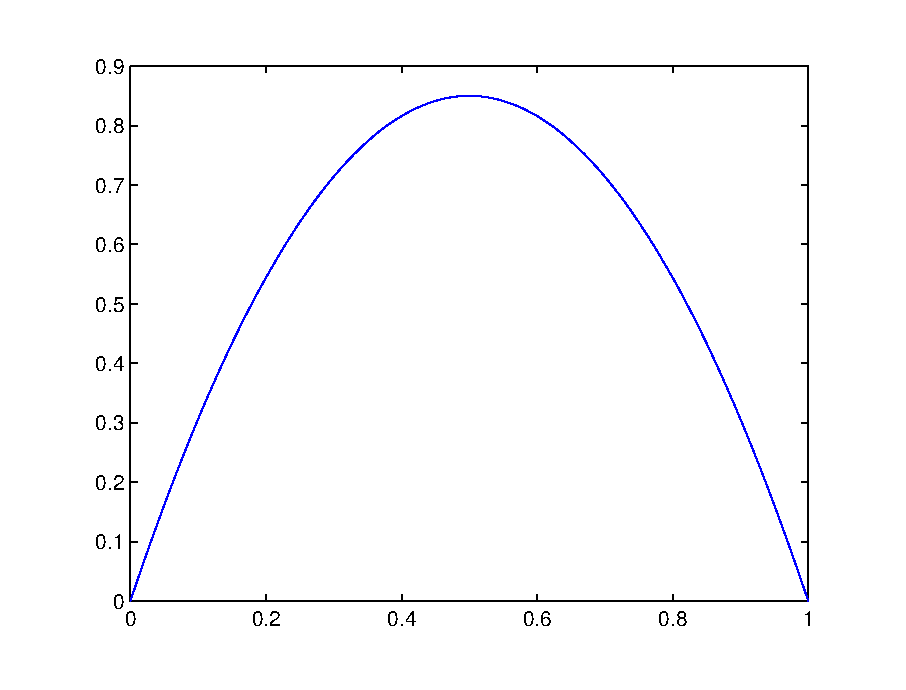
\includegraphics[width=0.5\textwidth]{../figs_01_intro_and_matlab/plot_iterates_1}
\end{center}
}


This is a very basic plot. 
We could want to plot more than one object (for example, the line $y=x$ would be nice).
\begin{verbatim}
plot(x,x,x,f(x,3.4));
\end{verbatim}
Ordering is by pairs: $x_1,f_1(x_1),x_2,f_2(x_2)$. Two elements in a pair {\bf must have} the same number of columns. Different pairs {\bf can have} different numbers of columns. Each element in a given pair can be a point, a vector, a matrix.

We could also want to label the axes.
\begin{verbatim}
xlabel('x');
ylabel('f(x)');
\end{verbatim}
\begin{center}
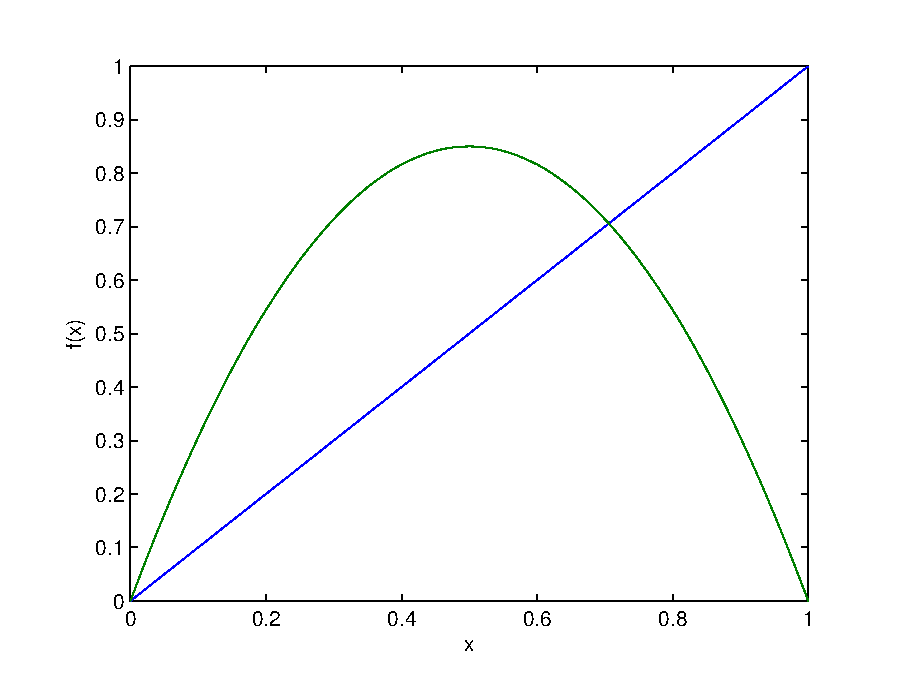
\includegraphics[width=0.5\textwidth]{../figs_01_intro_and_matlab/plot_iterates_2}
\end{center}

\frame{\frametitle{Computing several iterates}
For the moment, we only have $f(x)$. We want $f^n(x)$, for a given $n$. Several ways.
\begin{itemize}
\item Taking for example $r=3.5$, use
\begin{verbatim}
f(f(x,3.5),3.5)
\end{verbatim}
\item The downside to this method is that matlab does not allow to formally define $f^n$, so tricks have to be used for larger values of $n$, for example, produce a string containing the command 
\begin{verbatim}
f(f(f(f(f(x,3.5),3.5),3.5),3.5),3.5)
\end{verbatim}
and evaluate it. This is feasible but complicated.
\item Another method consists in using the result found at the previous step to evaluate the next. We do this now.
\end{itemize}
}


\frame{\frametitle{Automatic resizing of vectors and matrices}
We are going to use a very nice feature of matlab: adding elements to a vector, or rows/columns to a matrix, is automatic. Suppose for example that we had defined $x$ as
\begin{verbatim}
x=0:0.01:0.5;
\end{verbatim}
Then 
\begin{verbatim}
x=[x,0.51:0.01:1];
\end{verbatim}
would produce the vector $x$ as we had earlier.
}

\noindent{\bf Be careful!} Note that the command was
\begin{verbatim}
x=[x,0.51:0.01:1];
\end{verbatim}
that is, the old and new entries were separated by a ``,''. This is \emph{horizontal concatenation}. The command with a ``;'' tries to add a new row. In our case, we get
\begin{verbatim}
>> z=[z;0.51:0.01:1]
??? Error using ==> vertcat
All rows in the bracketed expression must have the same 
number of columns.
\end{verbatim}
because we are trying to add a row of 50 elements to a row of 51 elements. But
\begin{verbatim}
>> z=[z;0.51:0.01:1.01]
\end{verbatim}
works, and gives a $2\times 51$ matrix.


Here, we are going to use the latter form of the command, and add each successive iterate to a solution matrix $M$.
First, define an empty matrix,
\begin{verbatim}
M=[];
\end{verbatim}
Then we need to loop from 1 to $n$, where $n$ is the iterate that we want. 

\frame{\frametitle{Loops}
The command uses the same type of syntax as the creation of a vector: to loop from $4$ to $12$ by steps of 1,
\begin{verbatim}
for i=4:12,
   command(s) to be repeated, maybe using the value i
end;
\end{verbatim}
whereas to loop by non-unit or non-integer steps, say from 4 to 12 by steps of 1.35,
\begin{verbatim}
for i=4:1.35:12,
   command(s) to be repeated, maybe using the value i
end;
\end{verbatim}
Note that in that case, the last $i$ is equal to $10.75$, not $12$, since $10.75+1.35=12.1>12$. The same is true when using non-unit steps to create vectors.
}

\frame{\frametitle{Accessing matrix elements}
Suppose that $M$ is an $m\times n$-matrix. Then
\begin{itemize}
\item {\tt M(i,j)} is the element on the $i$th row and $j$th column.
\item {\tt M(i,:)} is the $i$th row.
\item {\tt M(:,j)} is the $j$th column. 
\item {\tt M(end,:)} is the last row of $M$ ({\tt end} is a reserved word which always points to the last valid index in a given matrix dimension).
\item {\tt M(:,end)} is the last column of $M$.
\item {\tt M(end,1:10)} are the first 10 entries in the last row of $M$.
\item {\tt M(1:2,3:5)} is the submatrix of $M$ consisting of rows 1 and 2 and columns 3 to 5 of $M$.
\end{itemize}
}


\frame{\frametitle{Back to the iterates}
After some thought, we realize that we will need to go back one iterate. So instead of starting with empty matrix $M$, fill the first row of $M$ with first iterate, and start at iterate 2.
\begin{verbatim}
n=10;
r=3.5;
M=f(x,r);
for i=2:n,
    M=[M;f(M(end,:),r)];
end;
plot(x,M);
\end{verbatim}
This plots all the iterates to $n$. The result is a bit crowded, as can be seen in Figure~\ref{fig:10_iterates_logistic}.
\begin{figure}[htbp]
\begin{center}
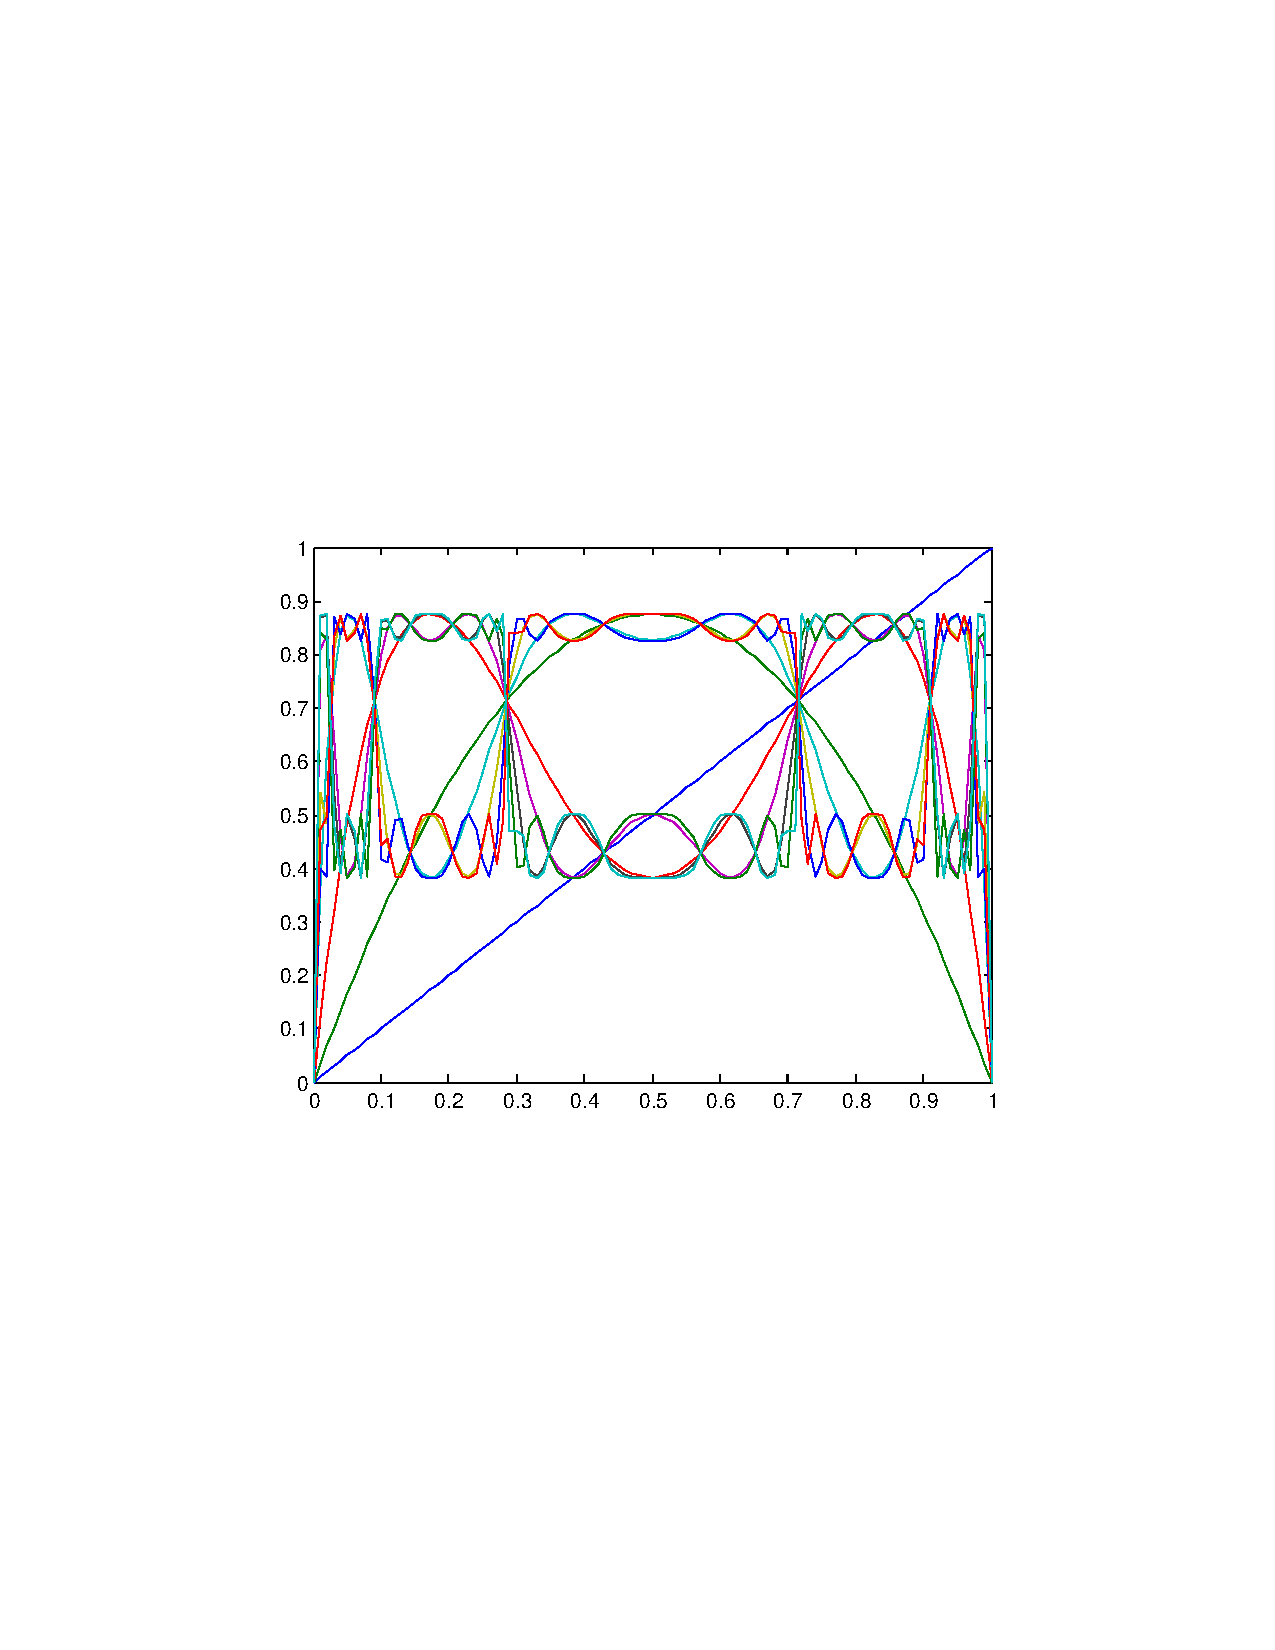
\includegraphics[width=0.5\textwidth]{../figs_01_intro_and_matlab/plot_iterates_3}
\caption{Plot of the first 10 iterates of the logistic map.}
\label{fig:10_iterates_logistic}
\end{center}
\end{figure}


\subsection{Numerical simulation of differential equations}

We want to compute the numerical solution to the logistic equation, which is given by
\begin{equation}\label{eq:ode_logistic_ident}
N'=rN\left(1-\frac NK\right),
\end{equation}
with $r$ the intrinsic growth rate of the population and $K$ the carrying capacity (see Chapter~\ref{chap:single_pop_growth} for details).
There are many ways to do this.
We can use, for example,
\begin{itemize}
\item matlab
\item octave
\item scilab
\item maple
\item mathematica
\item many others..
\end{itemize}
We recommend using matlab, octave or scilab are recommended because of their ``philosophy'',
which is very close to the ``natural'' way one proceeds with an ode. Note also that these programs are geared toward numerical simulations, and are therefore very efficient in that context.

A brief reminder about Euler's method helps to understand the above remark about the ``philosophy'' of the programs. The solution to the initial value problem
\begin{align*}
x' &= f(t,x) \\
x(t_0) &= x_0
\end{align*}
can be approximated numerically by the following sequence:
\begin{align*}
t_{k+1} &= t_k+h \\
x_{k+1} &= x_k+hf(t_k,x_k)
\end{align*}
for a time step $h>0$ and with first term $(t_0,x_0)$.
The techniques (a.k.a. ``numerical solvers'') in matlab are much more advanced, but the idea is the same: approximate the solution to an ODE by using a numerical algorithm that uses information on the ``shape'' of the vector field.
We need two files:
\begin{enumerate}
\item a RHS function defining $f(t,x)$
\item a function or command line statement that ``calls'' the RHS function with a numerical solver
\end{enumerate}
For the logistic equation \eqref{eq:ode_logistic_ident}, we could define the following function:
\begin{verbatim}
function dN=rhs_logistic(t,N,p)
% This function returns the value of dN/dt 
% at the point (t,N), using parameters in the 
% structure p

dN=p.r*N*(1-N/p.K);
\end{verbatim}
which we save in a file called, say, \verb%rhs_logistic.m%. Note that {\tt t} is required in the function arguments even if not used in the RHS function, i.e., even if $f$ is autonomous.

In our code above, the variable {\tt p} is defined as a \emph{structure}. This is a very useful construct in many programming languages. Think of it as a \emph{container}:
\begin{verbatim}
>> p.K=100;
>> p.r=2;
>> p
p =
    K: 100
    r: 2
\end{verbatim}
Pros: {\tt p} is passed to the function as one parameter, instead of a list of parameters. Cons: do not forget {\tt p.} in front of the parameter.
We will see later why structures are useful

Once the right hand side function is set up, we need to invoke the numerical solver.
The call is of the form (from the help): 
\begin{verbatim}
ode23, ode45, ode113, ode15s, ode23s, ode23t, ode23tb

Solve initial value problems for ordinary differential 
equations

Syntax
[T,Y] = solver(odefun,tspan,y0)
[T,Y] = solver(odefun,tspan,y0,options)
[T,Y,TE,YE,IE] = solver(odefun,tspan,y0,options)
sol = solver(odefun,[t0 tf],y0...)

where solver is one of ode45, ode23, ode113, ode15s, 
ode23s, ode23t, or ode23tb
\end{verbatim}
Typically, you can use {\tt ode45}


\frame{\frametitle{Computing the numerical solution to the logistic}
We call our solver as follows:
\begin{verbatim}
tspan=[1790 2000]; %The time span of the solution
IC=3.929;          %The initial condition (in 1790)
p.K=300;           %Set the parameters
p.r=0.5;
[t,N]=ode45(@rhs_logistic,tspan,IC,[],p);
\end{verbatim}
(The one before last argument, {\tt []}, represents the options structure. Here we are not modifying any option, and so pass an empty vector)
\vskip0.5cm
Save this file as, say, \verb%call_solver.m% 
\vskip0.5cm
After running it, we have a vector {\tt t} of times (covering {\tt tspan}) and a vector {\tt N} of solution
}

\frame[containsverbatim]{\frametitle{Plotting the solution}
\begin{verbatim}
plot(t,N)
\end{verbatim}
gives
\begin{figure}[htbp]
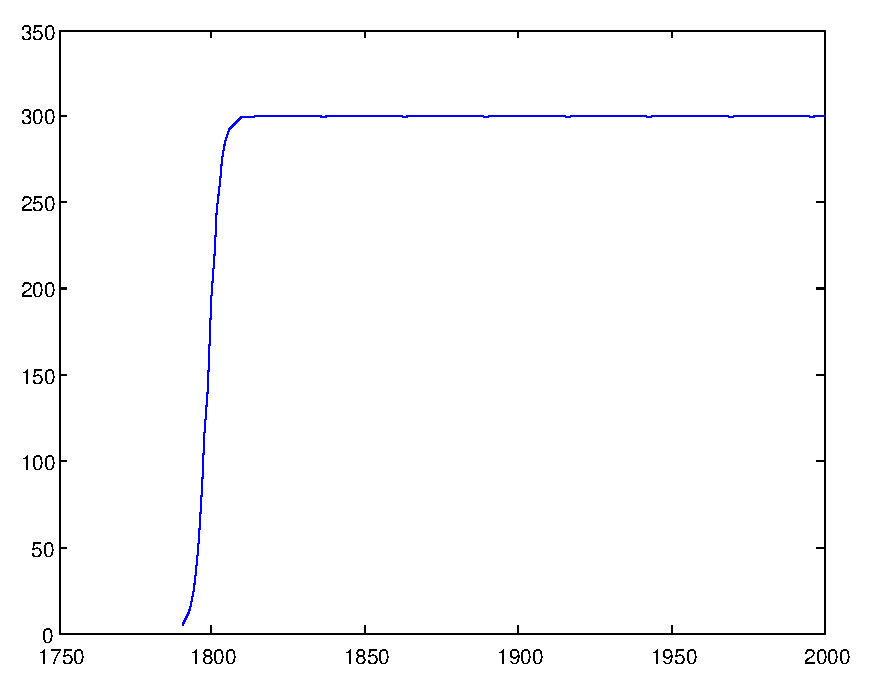
\includegraphics[width=0.7\textwidth]{../figs_09_parameter_identification/fig_logistic_ode_1}
\end{figure}
}

\frame[containsverbatim]{\frametitle{Tightening the $x$-axis}
\begin{verbatim}
plot(t,N)
xlim([t(1) t(end)])
\end{verbatim}
gives
\begin{figure}[htbp]
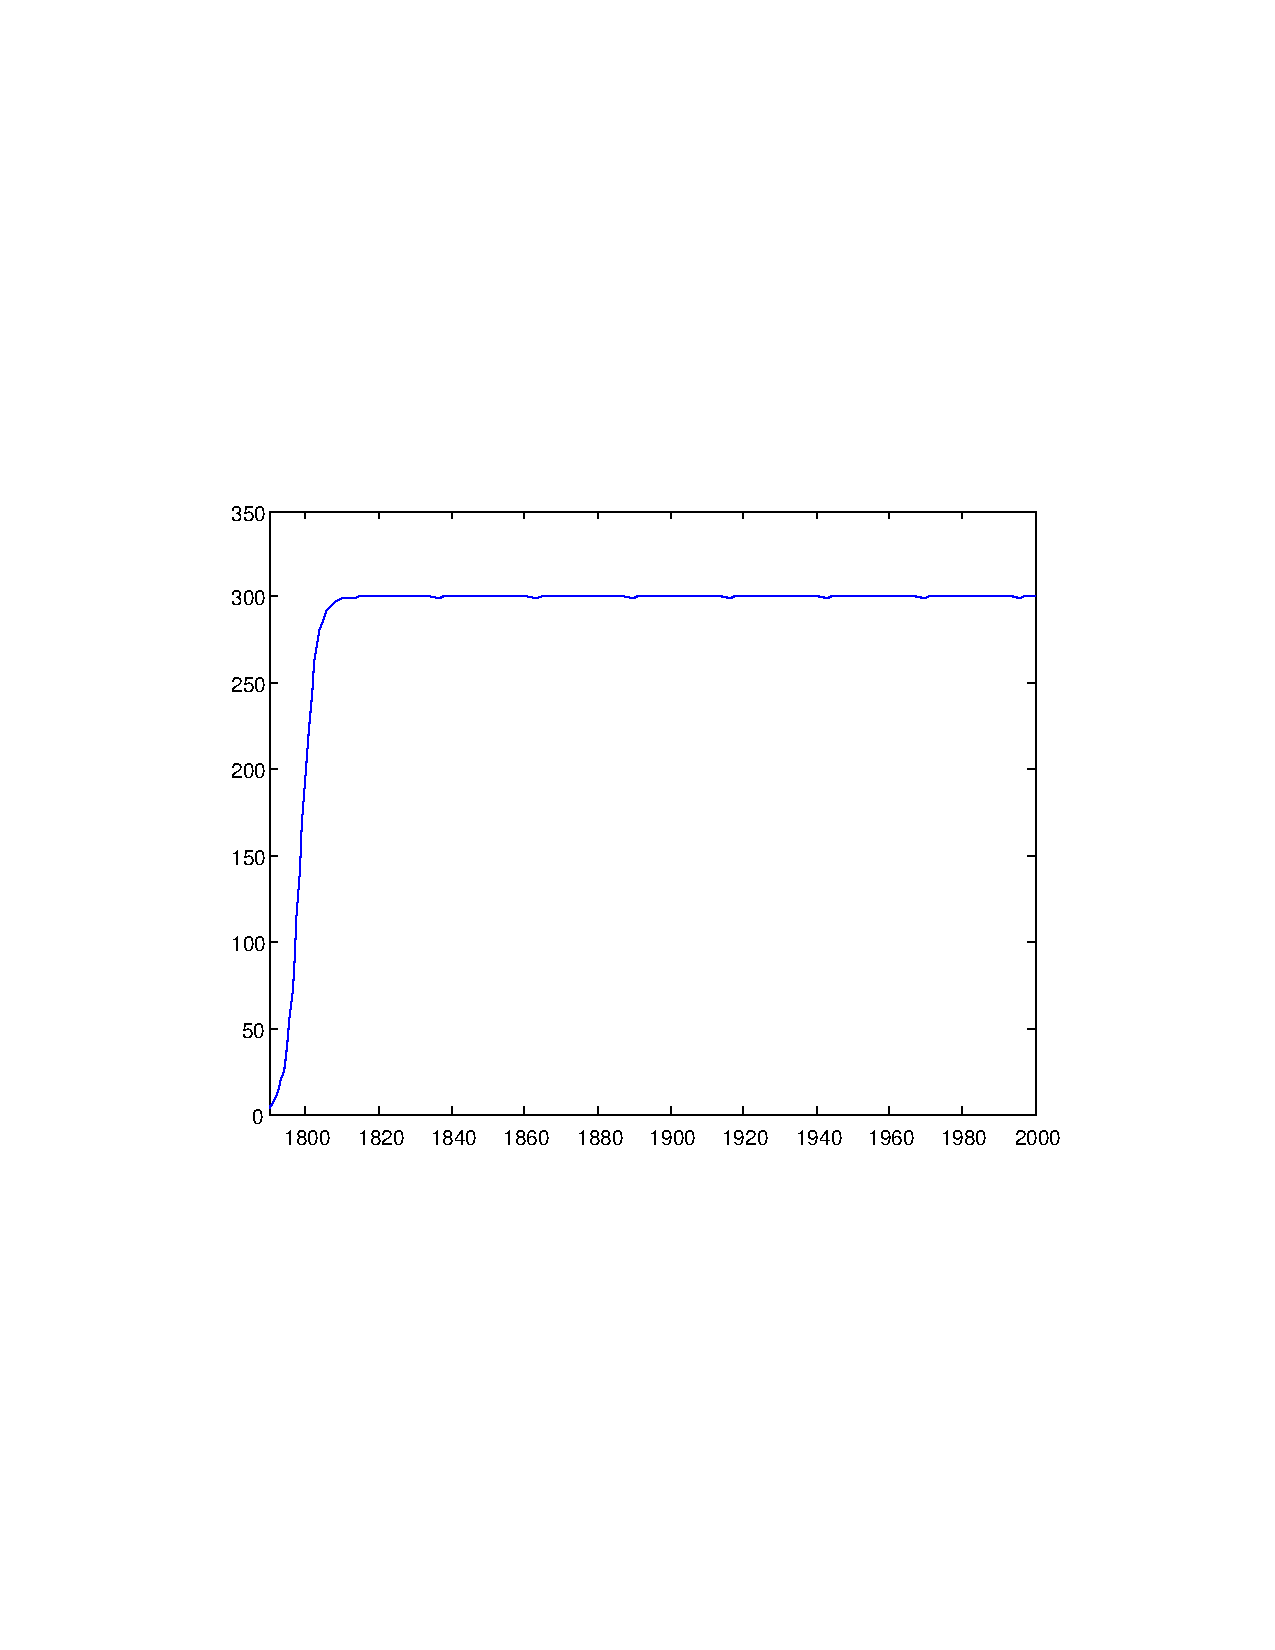
\includegraphics[width=0.7\textwidth]{../figs_09_parameter_identification/fig_logistic_ode_2}
\end{figure}
}

\frame[containsverbatim]{\frametitle{Using Octave}
The syntax in Octave is almost identical to the matlab syntax. In fact, if you use the additional programs in the {\tt forge} repository, a function {\tt ode45} is defined
\vskip0.5cm
However, the functions (in octave) do not implement the use of a parameter by default, so a work-around must be used
\vskip0.5cm
Update: as of V3.0 and using ode45, parameters can be passed and the matlab code given before works, with the following little modification:
\begin{verbatim}
opt=odeset('InitialStep',0.05,'MaxStep',1);
[t,N]=ode45(@rhs_logistic,tspan,IC,opt,p);
\end{verbatim}
which makes sure that the time step does not become too large)
}


\frame[containsverbatim]{\frametitle{Using scilab}
The syntax in scilab differs a little from matlab, so beware.
\begin{verbatim}
function ydot=f(t,y);
ydot=y^2-y*sin(t)+cos(t);
endfunction
\end{verbatim}
}


\chapter{Single population growth models}
\label{chap:single_pop_growth}



\section{Objectives}
We are given a table with the population census at different time intervals between a date $a$ and a date $b$, and want to get an expression for the population. This allows us to: 
\begin{itemize}
\item compute a value for the population at any time between the date $a$ and the date $b$ (\textbf{interpolation}),
\item predict a value for the population at a date before $a$ or after $b$ (\textbf{extrapolation}).
\end{itemize}

%\begin{figure}[htbp]
%\begin{center}
%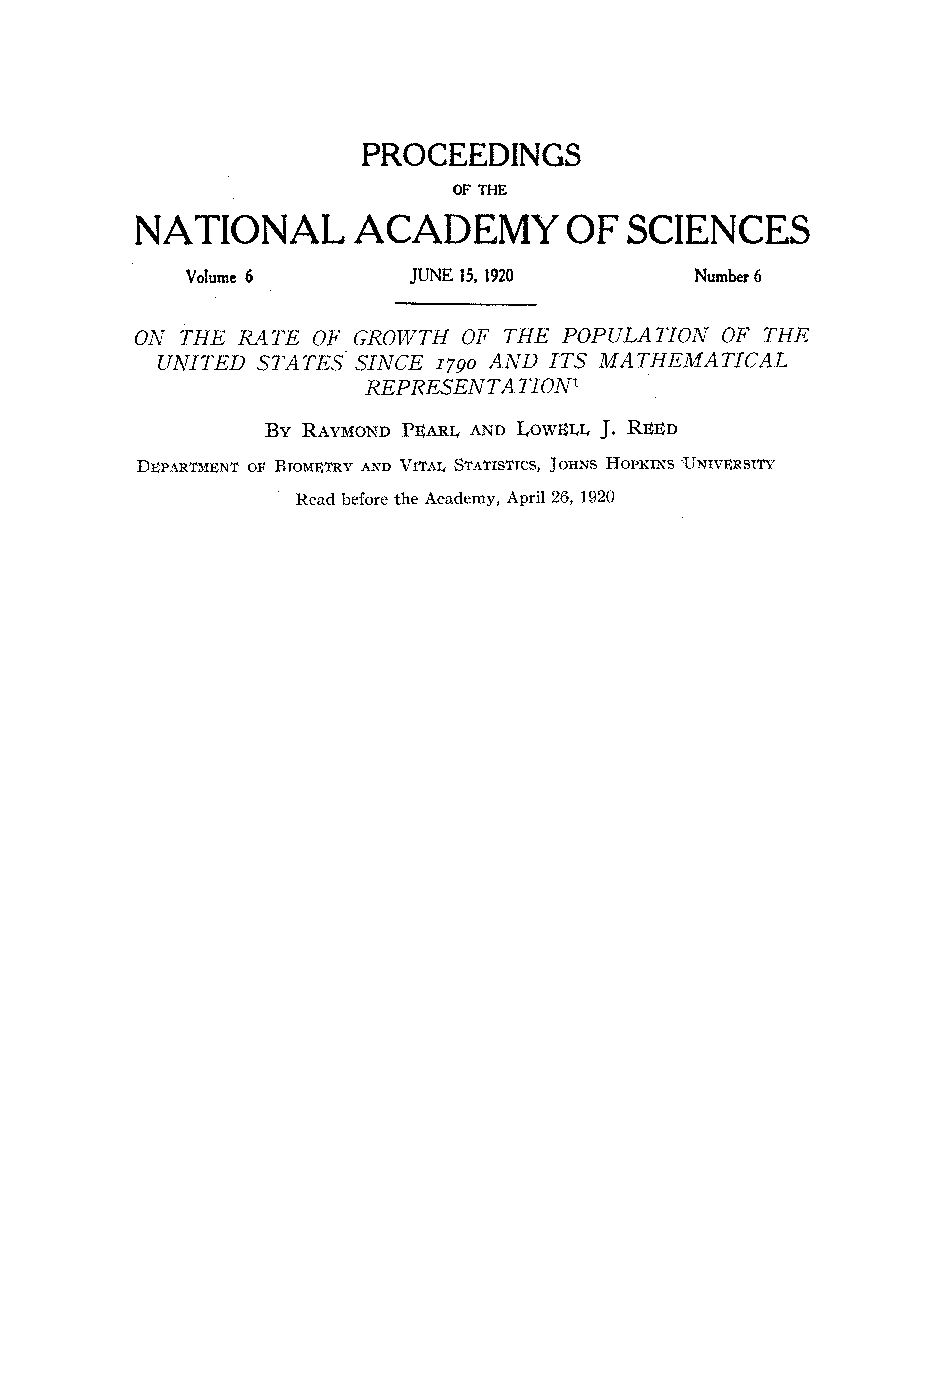
\includegraphics[width=0.7\textwidth]{../figs_02_population_growth/titre_PearlReed1920PNAS6}
%\end{center}
%\end{figure}

This was studied in a series of papers in the 1920-40's, mainly under the influence of Pearl and Reed \cite{PearlReed1920,PearlReed1930,PearlReedFish1940}.


\section{The data: US census}
% \begin{figure}[htbp]
% \begin{center}
% 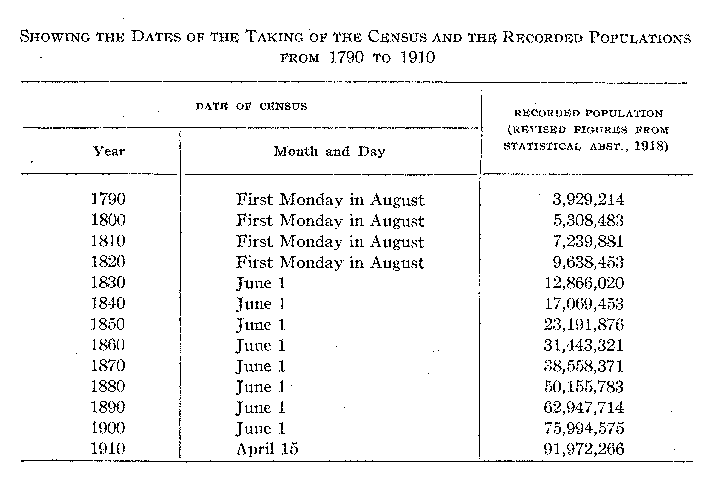
\includegraphics[width=0.8\textwidth]{../figs_02_population_growth/table_PearlReed1920PNAS6}
% \end{center}
% \end{figure}



\begin{table}[htbp]
\begin{center}
\begin{tabular}{cc}
Year & Population\\
& (millions) \\
\hline
1790 & 3.929 \\
1800 & 5.308 \\
1810 & 7.240 \\
1820 & 9.638 \\
1830 & 12.866 \\
1840 & 17.069 \\
1850 & 23.192 \\
1860 & 31.443 \\
1870 & 38.558 \\
1880 & 50.156 \\
1890 & 62.948 \\
1900 & 75.995 \\
1910 & 91.972 
\end{tabular}
\caption{The US population from 1790 to 1910. From Pearl and Reed
\cite{PearlReed1920}.}
\label{table:US_population_1790_1910}
\end{center}
\end{table}

Using MatLab (or Octave), create two vectors using commands such as
\begin{verbatim}
t=1790:10:1910;
\end{verbatim}
which creates the vector of time points, and 
\begin{verbatim}
P=[3929214,5308483,7239881,9638453,12866020, ...
    17069453,23191876,31443321,38558371,50155783, ...
    62947714,75994575,91972266];
\end{verbatim}
for corresponding population values ({\tt ...} indicates that the line continues below).
Then plot using
\begin{verbatim}
plot(t,P);
\end{verbatim}
\begin{center}
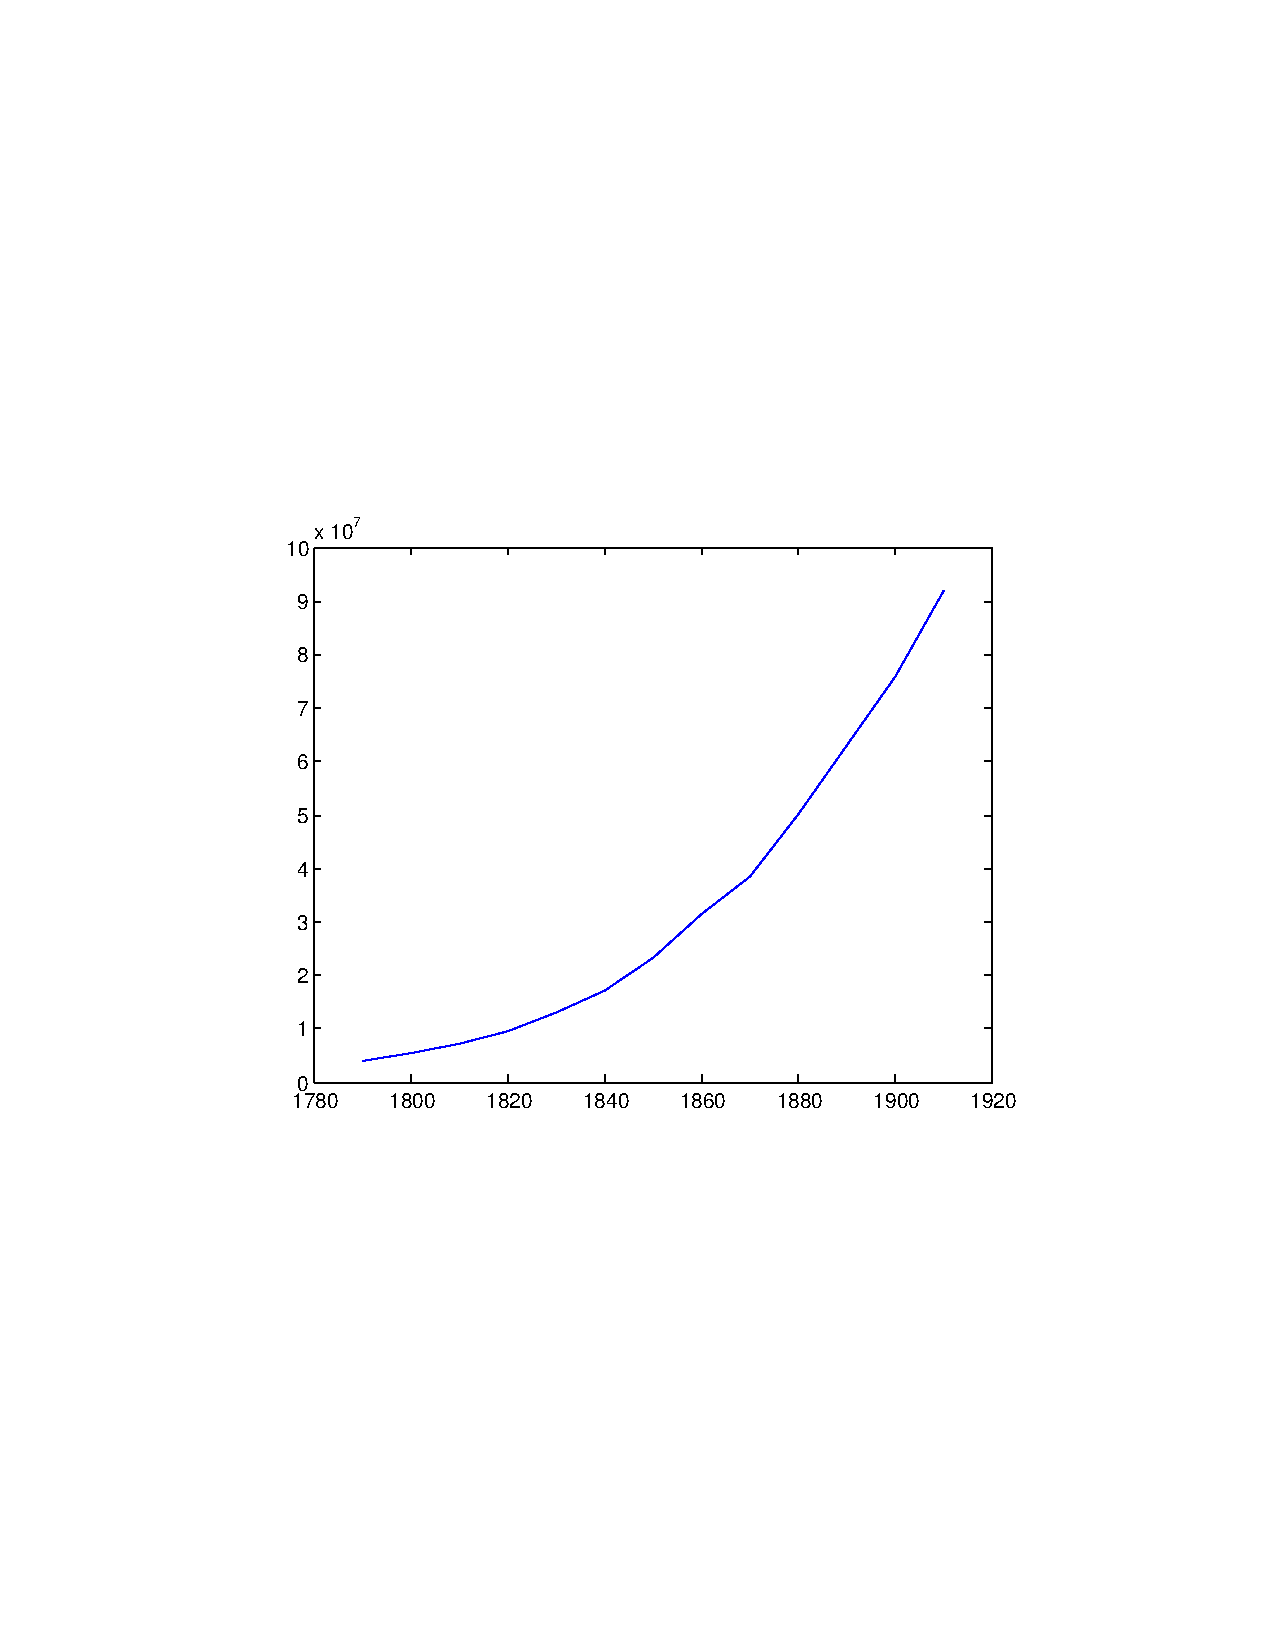
\includegraphics[width=0.5\textwidth]{../figs_02_population_growth/USpop_to1910}
\end{center}
To get points instead of a line, use the command
\begin{verbatim}
plot(t,P,'*');
\end{verbatim}
\begin{center}
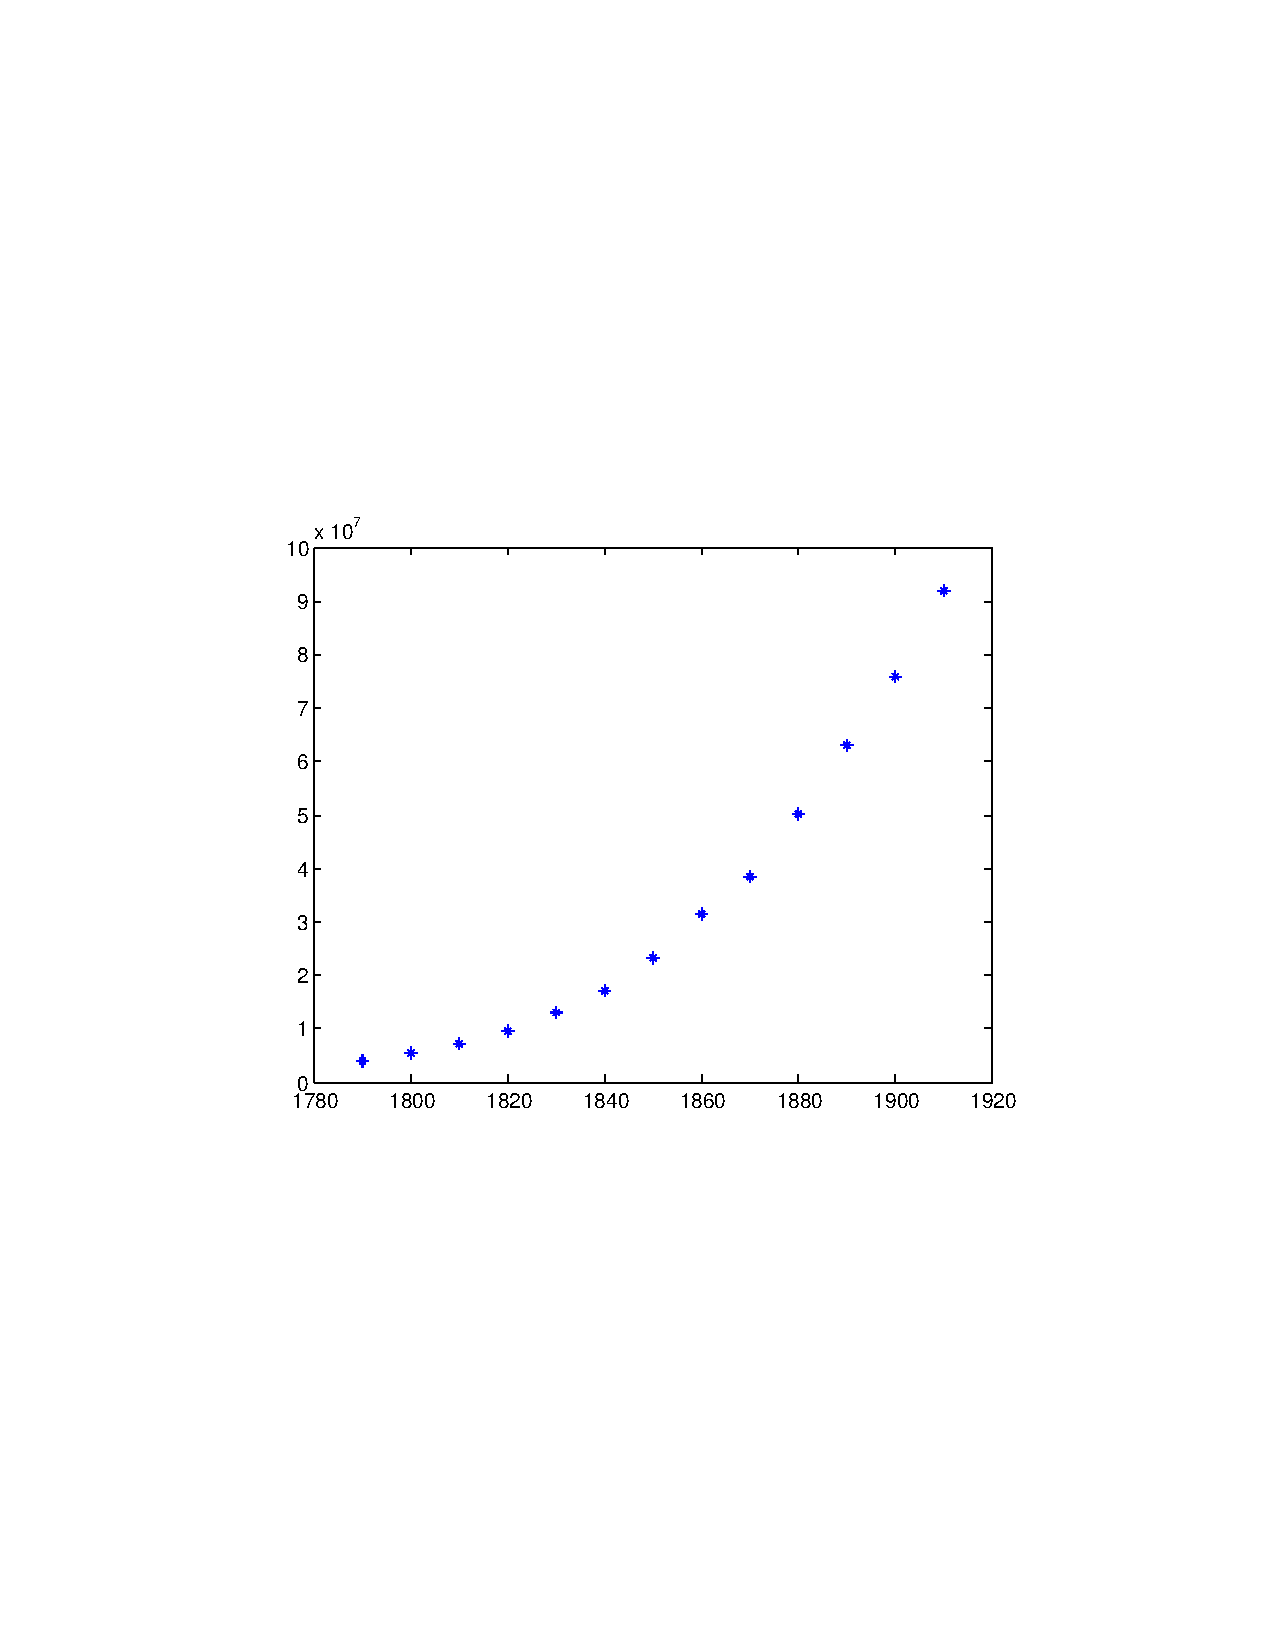
\includegraphics[width=0.5\textwidth]{../figs_02_population_growth/USpop_to1910_points}
\end{center}

\subsection{A quadratic curve?}
The curve looks like part of a parabola. So let us use nonlinear regression to fit a curve of the form
\[
P(t)=a+bt+ct^2
\]
to the data.
We proceed as follows.
There are 13 data points which we denote $(t_k,P_k)$ for $k=1,\ldots,13$. The objective of nonlinear regression is to find the values of $a,b,c$ such that
\[
S=\sum_{k=1}^{13} \left(P(t_k)-P_k\right)^2
\]
be minimal. This means that the values $a,b,c$ are such that the square of the distance between the the known points $(t_k,P_k)$ and those for corresponding times, $(t_k,P(t_k))=(t_k,a+bt_k+ct_k^2)$, is minimal. To emphasize the dependence of $S$ on the values of $a,b,c$, we denote it
\[
S(a,b,c)=\sum_{k=1}^{13} \left(a+bt_k+ct_k^2-P_k\right)^2.
\]
We have that $S(a,b,c)$ is minimal if (necessary condition) $\partial S/\partial a=\partial S/\partial b=\partial S/\partial c=0$, with
\begin{align*}
\frac{\partial S}{\partial a} &= 2\sum_{k=1}^{13}(a+bt_k+ct_k^2-P_k) \\
\frac{\partial S}{\partial b} &= 2\sum_{k=1}^{13}(a+bt_k+ct_k^2-P_k)t_k \\
\frac{\partial S}{\partial c} &= 2\sum_{k=1}^{13}(a+bt_k+ct_k^2-P_k)t_k^2.
\end{align*}
So we want
\begin{align*}
2\sum_{k=1}^{13}(a+bt_k+ct_k^2-P_k) &= 0\\
2\sum_{k=1}^{13}(a+bt_k+ct_k^2-P_k)t_k &= 0 \\
2\sum_{k=1}^{13}(a+bt_k+ct_k^2-P_k)t_k^2 &= 0,
\end{align*}
which we can simplify,
\begin{align*}
\sum_{k=1}^{13}(a+bt_k+ct_k^2-P_k) &= 0\\
\sum_{k=1}^{13}(a+bt_k+ct_k^2-P_k)t_k &= 0 \\
\sum_{k=1}^{13}(a+bt_k+ct_k^2-P_k)t_k^2 &= 0.
\end{align*}
Rearranging the system, we get
\begin{align*}
\sum_{k=1}^{13}(a+bt_k+ct_k^2) &= \sum_{k=1}^{13}P_k\\
\sum_{k=1}^{13}(at_k+bt_k^2+ct_k^3) &= \sum_{k=1}^{13}P_kt_k\\
\sum_{k=1}^{13}(at_k^2+bt_k^3+ct_k^4) &= \sum_{k=1}^{13}P_kt_k^2.
\end{align*}
After a bit of tidying up, and emphasizing the fact that the unknowns are $a,b,c$, we get
\begin{align*}
\left(\sum_{k=1}^{13}1\right)a+\left(\sum_{k=1}^{13}t_k\right)b+\left(\sum_{k=1}^{13}t_k^2\right)c &= \sum_{k=1}^{13}P_k \\
\left(\sum_{k=1}^{13}t_k\right)a+\left(\sum_{k=1}^{13}t_k^2\right)b+\left(\sum_{k=1}^{13}t_k^3\right)c &= \sum_{k=1}^{13}P_kt_k \\
\left(\sum_{k=1}^{13}t_k^2\right)a+\left(\sum_{k=1}^{13}t_k^3\right)b+\left(\sum_{k=1}^{13}t_k^4\right)c &= \sum_{k=1}^{13}P_kt_k^2.
\end{align*}
So we need to solve the linear system
\[
\begin{pmatrix}
13 & \sum\limits_{k=1}^{13}t_k & \sum\limits_{k=1}^{13}t_k^2 \\
\sum\limits_{k=1}^{13}t_k & \sum\limits_{k=1}^{13}t_k^2 & \sum\limits_{k=1}^{13}t_k^3 \\
\sum\limits_{k=1}^{13}t_k^2 & \sum\limits_{k=1}^{13}t_k^3 & \sum\limits_{k=1}^{13}t_k^4
\end{pmatrix}
\begin{pmatrix}
a\\ b\\ c
\end{pmatrix}
=
\begin{pmatrix}
\sum\limits_{k=1}^{13}P_k \\
\sum\limits_{k=1}^{13}P_kt_k \\
\sum\limits_{k=1}^{13}P_kt_k^2
\end{pmatrix}.
\]
With MatLab (or Octave), getting the values is easy.
\begin{itemize}
\item To apply an operation to every element in a vector or matrix, prefix the operation with a dot, hence
\begin{verbatim}
 t.^2;
\end{verbatim}
gives, for example, the vector with every element $t_k$ squared. 
\item Also, the function {\tt sum} gives the sum of the entries of a vector or matrix.
\item When entering a matrix or vector, separate entries on the same row by {\tt ,} and create a new row by using {\tt ;}.
\end{itemize}
Thus, to set up the problem in the form of solving $Ax=b$, we need to do the
following:
\begin{verbatim}
format long g;
A=[13,sum(t),sum(t.^2);sum(t),sum(t.^2),sum(t.^3);...
sum(t.^2),sum(t.^3),sum(t.^4)];
b=[sum(P);sum(P.*t);sum(P.*(t.^2))];
\end{verbatim}
The {\tt format long g} command is used to force the display of digits (normally, what is shown is in ``scientific'' notation, not very informative here). 

Then, solve the system using
\begin{verbatim}
A\b
\end{verbatim}
We get the following output:
\begin{verbatim}
>> A\b
Warning: Matrix is close to singular or badly scaled.
         Results may be inaccurate. RCOND = 1.118391e-020.

ans =
        22233186177.8195
        -24720291.325476
        6872.99686313725
\end{verbatim}
(note that here, Octave gives a solution that is not as good as this one, provided by MatLab).


\subsection{Checking our results for the quadratic}
Thus
\[
P(t)=22233186177.81-24720291.32t+6872.99t^2
\]
To see what this looks like,
\begin{verbatim}
plot(t,22233186177.81-24720291.32.*t+6872.99.*t.^2);
\end{verbatim}
(note the dots before multiplication and power, since we apply this function to every entry of $t$).
In fact, to compare with original data:
\begin{verbatim}
plot(t,22233186177.81-24720291.32.*t+6872.99.*t.^2,t,P,'*');
\end{verbatim}
\begin{figure}[htbp]
\begin{center}
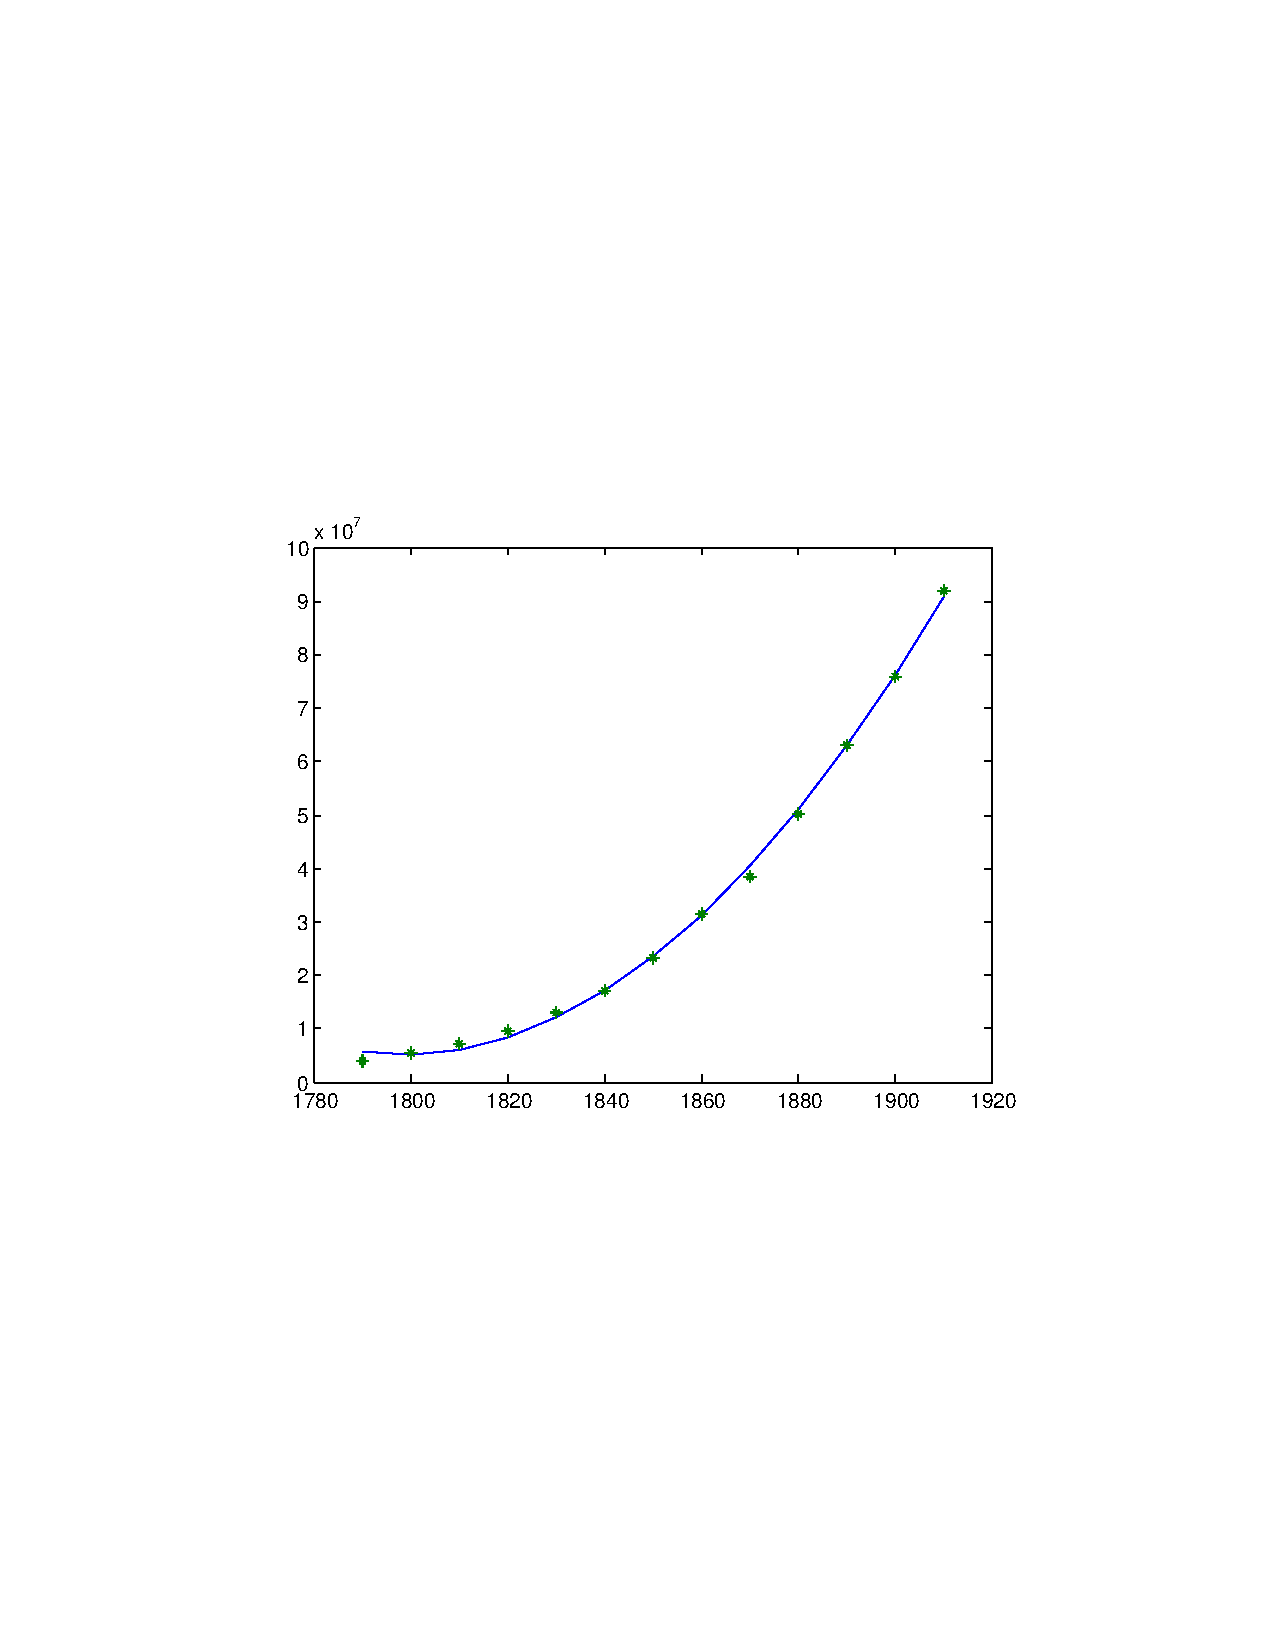
\includegraphics[width=0.5\textwidth]
{../figs_02_population_growth/quadratic_fit}
\end{center}
\end{figure}




Now we want to generate the table of values, to compare with the true values and thus compute the error. To do this, we can proceed directly:
\begin{verbatim}
computedP=22233186177.81-24720291.32.*t+6872.99.*t.^2;
\end{verbatim}
We get
\begin{verbatim}
computedP =
 Columns 1 through 4:
      5633954.39      5171628.52      6083902.03    8370774.90
 Columns 5 through 8:
      12032247.15      17068318.78      23478989.77    31264260.14
 Columns 9 through 12:
       40424129.88      50958598.99      62867667.48    76151335.34
 Column 13:
      90809602.57
\end{verbatim}

We can also create an \textbf{inline} function
\begin{verbatim}
f=inline('22233186177.81-24720291.32.*t+6872.99.*t.^2')
f =
     Inline function:
     f(t) = 22233186177.81-24720291.32.*t+6872.99.*t.^2
\end{verbatim}
This function can then easily be used for a single value
\begin{verbatim}
octave:24> f(1880)
ans =     50958598.9969215
\end{verbatim}
as well as for vectors.

(Recall that $t$ has the dates; $t$ in the definition of the function is a dummy
variable, we could have used another letter-.)
\begin{verbatim}
octave:25> f(t)
ans =
 Columns 1 through 4:
      5633954.39      5171628.52      6083902.03    8370774.90
 Columns 5 through 8:
      12032247.15      17068318.78      23478989.77    31264260.14
 Columns 9 through 12:
       40424129.88      50958598.99      62867667.48    76151335.34
 Column 13:
      90809602.57
\end{verbatim}
Form the vector of errors, and compute sum of errors squared:
\begin{verbatim}
octave:26> E=f(t)-P;
octave:27> sum(E.^2)
ans =     12186176863781.4
\end{verbatim}
Quite a large error (12,186,176,863,781.4), which is normal since we have used actual numbers, not thousands or millions of individuals, and we are taking the square of the error.

To present things legibly, one way is to put everything in a matrix..
\begin{verbatim}
M=[P;f(t);E;E./P];
\end{verbatim}
This matrix will have each type of information as a row, so to display it in the form of a table, show its transpose, which is achieved using the function {\tt transpose} or the operator $'$.
\begin{verbatim}
M'
ans =
 3929214      5633954.39      1704740.39     0.43
 5308483      5171628.52     -136854.47     -0.02
 7239881      6083902.03     -1155978.96    -0.15
 9638453      8370774.90     -1267678.09    -0.13
12866020      12032247.15     -833772.84   -0.06
17069453      17068318.78     -1134.21  -6.644728828e-05
23191876      23478989.77      287113.77    0.01
31443321      31264260.14     -179060.85  -0.00569471832254123
38558371      40424129.88      1865758.88    0.04
50155783      50958598.99      802815.99    0.01
62947714      62867667.48     -80046.51  -0.00127163502018304
75994575      76151335.34      156760.34   0.00206278330494212
91972266      90809602.57     -1162663.42    -0.01
\end{verbatim}


\frame{\frametitle{Now for the big question...}
How does our formula do for present times?
\begin{verbatim}
f(2006)
ans =     301468584.066013
\end{verbatim}
Actually, quite well: 301,468,584, compared to the 298,444,215 July 2006 estimate, overestimates the population by 3,024,369, a relative error of approximately 1\%.
}

\frame{\frametitle{The US population from 1790 to 2000 (revised numbers)}
\begin{center}
\begin{tabular}[t]{ccc}
\begin{tabular}{cc}
Year & Population\\
& (millions) \\
\hline
1790 & 3.929 \\
1800 & 5.308 \\
1810 & 7.240 \\
1820 & 9.638 \\
1830 & 12.866 \\
1840 & 17.069 \\
1850 & 23.192 \\
1860 & 31.443 \\
1870 & 38.558 \\
1880 & 50.156 \\
1890 & 62.948
\end{tabular} 
&\quad &
\begin{tabular}{cc}
Year & Population \\
& (millions) \\
\hline
1900 & 76.212 \\
1910 & 92.228 \\
1920 & 106.021 \\
1930 & 123.202 \\
1940 & 132.164 \\
1950 & 151.325 \\
1960 & 179.323 \\
1970 & 203.302 \\
1980 & 226.542 \\
1990 & 248.709 \\
2000 & 281.421
\end{tabular}
\end{tabular}
\end{center}
}

\subsection{Other similar approaches -- The logistic curve}
Pritchett \cite{Pritchett1891} tried
\[
P=a+bt+ct^2+dt^3,
\]
using data from 1790 to 1880 (inclusive).
%We have done this one, and found it to be quite good too.
Pearl and Reed, in \cite{PearlReed1920}, start by comparing the results of \cite{Pritchett1891} with those found by using 
\[
P(t)=a+bt+ct^2+d\ln t.
\]
They find
\[
P(t)=9,064,900-6,281,430t+842,377t^2+19,829,500\ln t.
\]
and a cumulative error ($S$) half of that of Pritchett.
They then try
\[
P(t)=\frac{be^{at}}{1+ce^{at}}
\]
or
\begin{equation}\label{eq:logistic_curve}
P(t)=\frac{b}{e^{-at}+c}.
\end{equation}
They find
\[
P(t)=\frac{2,930.3009}{e^{-0.0313395t}+0.014854}.
\]


\section{The ODE logistic equation}
\label{sec:ODE_logistic}

The \emph{logistic curve} \eqref{eq:logistic_curve} is the solution to an \emph{ordinary differential equation} called the \textbf{logistic equation}.
This equation was introduced by Pierre-Fran\c{c}ois Verhulst
(1804-1849) \cite{Verhulst1838,Verhulst1845}.
The idea is to represent a population evolving subject to the following effects:
\begin{itemize}
\item birth, at the \textbf{per capita} rate $b$,
\item death, at the \textbf{per capita} rate $d$,
\item competition of individuals with other individuals reduces their ability to survive, resulting in death.
\end{itemize}
This gives
\[
N'=bN-dN-\textrm{competition}.
\]
Competition describes the mortality that occurs when two individuals meet:
\begin{itemize}
\item
In chemistry, if there is a concentration $X$ of one product and $Y$ of another product, then $XY$, called \textbf{mass action}, describes the number of interactions of molecules of the two products.
\item
Here, we assume that $X$ and $Y$ are of the same type (individuals). So there are $N^2$ contacts.
\item 
These $N^2$ contacts lead to the death of individuals at the rate $c$.
\end{itemize}
Therefore, the \textbf{logistic} equation is
\begin{equation}\label{eq:ODE_logistic_second_form}
N'=bN-dN-cN^2.
\end{equation}
Rewriting this equation as
\[
N'=(b-d)N-cN^2,
\]
we see that 
\begin{itemize}
\item $b-d$ is the rate at which the population increases (or decreases) in the absence of competition. It is called the \textbf{intrinsic growth rate} of the population.
\item $c$ is the rate of \textbf{intraspecific} competition. The prefix \textbf{intra} refers to the fact that the competition is occurring between members of the same species, that is, within the species.\newline
[We will see later examples of \textbf{interspecific} competition, that is, between different species.]
\end{itemize}
Factor out an $N$ in \eqref{eq:ODE_logistic_second_form}, giving
\[
N'=\bigl((b-d)-cN\bigr)N.
\]
This gives us the original interpretation of the logistic equation, since, writing
\[
\frac{N'}N=(b-d)-cN,
\]
we have $N'/N$, the \textbf{per capita growth rate} of $N$, given by a constant, $b-d$, minus a \textbf{density dependent inhibition} factor, $cN$.

But the form \eqref{eq:ODE_logistic_second_form} is not the most well known form of the logistic equation. To obtain the most frequently used form, we transform \eqref{eq:ODE_logistic_second_form} as follows:
\begin{align*}
N' &= (b-d)N-cN^2\\
&= \bigl((b-d)-cN\bigr)N \\
&= \left(r-\frac rr cN\right)N,\quad\textrm{setting }r=b-d \\
&= rN\left(1-\frac crN\right) \\
&= rN\left(1-\frac NK\right),
\end{align*}
with
\[
\frac cr=\frac 1K.
\]
So, using the change of variables 
\[
(r,K)\leftrightarrow\left(b-d,\frac{b-d}c\right),
\]
we transform \eqref{eq:ODE_logistic_second_form} into the commonly used form
\begin{equation}\label{eq:ODE_logistic}
N'=rN\left(1-\frac NK\right),
\end{equation}
The parameter $r$ is the \textbf{intrinsic growth rate}, $K$ is the \textbf{carrying capacity}.
There are three ways to tackle this equation:
\begin{enumerate}
\item The equation is separable. [explicit method]
\item The equation is a Bernoulli equation. [explicit method]
\item Use qualitative analysis.
\end{enumerate}

\subsection{Solving the logistic as a separable equation}
\subsection{Solving the equation as a Bernoulli equation}

\subsection{Qualitative analysis of the logistic equation}
We study \eqref{sec:ODE_logistic}.
For this, write
\[
f(N)=rN\left(1-\frac NK\right),
\]
and consider the initial value problem (IVP) 
\begin{equation}\label{ivp:logistic_ode}
\begin{aligned}
N' &= f(N)\\
N(0) &= N_0\geq 0.
\end{aligned}
\end{equation}
The function $f$ is $C^1$ (differentiable with continuous derivative) so solutions to \eqref{ivp:logistic_ode} exist and are unique, by virtue of Theorem~\ref{th:existence_uniqueness_Cauchy}.
\textbf{Equilibria} of \eqref{eq:ODE_logistic} are points such that $f(N)=0$ (so that $N'=f(N)=0$, meaning $N$ does not vary). So we solve $f(N)=0$ for $N$. We find two points:
\begin{itemize}
\item $N=0$,
\item $N=K$.
\end{itemize}

We then consider the \textbf{well-posedness} of the problem, which consists in ensuring that solutions remain nonnegative (we are modelling populations) and bounded. This is usually carried out before any other type of analysis, but here, we use information derived from the nature of the equilibrium $N=0$.

By uniqueness of solutions to \eqref{ivp:logistic_ode}, solutions cannot cross the curve $N(t)=0$ (nor the curve $N(t)=K$, but this is not required for well-posedness). $N(t)=0$ is a solution to \eqref{ivp:logistic_ode}, defined for all $t\geq 0$. Suppose that, for a solution through $N_0>0$, there exists $t=\tau>0$ such that $N(\tau)=0$, and that $\tau$ is the first value of $t$ such that $N(t)=0$ (recall that $N_0>0$). Then, at the point $(t,N)=(\tau,0)$, we have two solutions: the solution through $(t,N)=(0,0)$ and the solution through $(t,N)=(0,N_0)$. This is a contradiction, since solutions are known to be unique (and thus, through a given point $(t,N)$, there is one, and one only, solution to \eqref{ivp:logistic_ode}).
Boundedness is easy to eastablish: remark that if $N>K$, then $f(N)<0$, implying that solutions decrease for $N>K$.


For the general behavior of solutions, there are several cases to consider.
\begin{itemize}
\item If $N_0=0$, then $N(t)=0$ for all $t\geq 0$, and from the above discussion, no solution with positive initial condition will ever reach zero.
\item $N\in(0,K)$, then $rN>0$ and $N/K<1$ so $1-N/K>0$, which implies that $f(N)>0$. As a consequence, $N(t)$ increases if $N_0\in(0,K)$.
\item If $N_0=K$, then $N(t)=K$ for all $t\geq 0$.
\item If $N>K$, then $rN>0$ and $N/K>1$, implying that $1-N/K<0$ and in turn, $f(N)<0$. As a consequence, $N(t)$ decreases if $N_0\in(K,+\infty)$.
\end{itemize}
Therefore, since the curve $N=K$ cannot be crossed, 
\begin{theorem}
Suppose that $N_0>0$. Then the solution $N(t)$ of \eqref{ivp:logistic_ode} is such that
\[
\lim_{t\to\infty} N(t)=K,
\]
so that $K$ is the number of individuals that the environment can support, the \textbf{carrying capacity} of the environment.

If $N_0=0$, then $N(t)=0$ for all $t\geq 0$.
\end{theorem}


\section{The delayed logistic equation}
\label{sec:DDE_logistic}
Consider the logistic equation \eqref{eq:ODE_logistic_second_form} written as
\[
\frac{N'}{N}=(b-d)-cN.
\]
Suppose that instead of instantaneous inhibition, there is a time delay $\tau$ between the instant the inhibiting event takes place and the moment when it affects the growth rate.
For example, two individuals fight for food, and one later dies of the injuries sustained during this fight. 

Reasonning as above, Hutchinson introduced in \cite{Hutchinson1948} a delayed logistic equation. In the case of a time $\tau$ between inhibiting event and inhibition, the equation above would be written as 
\[
\frac{N'}N=(b-d)-cN(t-\tau).
\]
Using the change of variables introduced in the ordinary differential equation case, this is written
\begin{equation}\label{eq:logistic_dde}
N'(t)=rN(t)\left(1-\frac{N(t-\tau)}K\right).
\end{equation}
Such an equation is called a \textbf{delay} differential equation. It is much more complicated to study than \eqref{eq:ODE_logistic}. In fact, although \eqref{eq:ODE_logistic} and \eqref{eq:logistic_dde} look very similar and that \eqref{eq:logistic_dde} has been studied for about 60 years now, there are details about \eqref{eq:logistic_dde} that remain unknown to this day.

\paragraph{Delayed initial value problem}
The IVP takes the form
\begin{equation}\label{ivp:logistic_dde}
\begin{aligned}
N'(t)&= rN(t)\left(1-\frac{N(t-\tau)}K\right),\\
N(t) &= \phi(t)\textrm{ for }t\in[-\tau,0],
\end{aligned}
\end{equation}
where $\phi(t)$ is some continuous function. Hence, initial conditions (called initial data in this case) must be specified on an interval, instead of being specified at a point, to guarantee existence and uniqueness of solutions.

We will not learn how to study this type of equation (this is graduate level mathematics). I will give a few results.

\vskip0.5cm
To find equilibria, remark that delay should not play a role, since $N$ should be constant. Thus, equilibria are found by considering the equation with no delay, which is \eqref{eq:ODE_logistic}.
\begin{theorem}
Suppose that $r\tau<\pi/2$. Then solutions of \eqref{ivp:logistic_dde} with positive initial data $\phi(t)$ starting close enough to $K$ tend to $K$. If $r\tau<37/24$, then all solutions of  \eqref{ivp:logistic_dde} with positive initial data $\phi(t)$ tend to $K$. If $r\tau>\pi/2$, then $K$ is an unstable equilibrium and all solutions of \eqref{ivp:logistic_dde} with positive initial data $\phi(t)$ on $[-\tau,0]$ are oscillatory.
\end{theorem}
There is a gray zone between $37/24$ ($\simeq 1.5417$) and $\pi/2$ ($\simeq 1.5708$). The global aspect was proved for $r\tau<37/24$ in 1945 by Wright \cite{Wright1955}. Although there is very strong numerical evidence that this is in fact true up to $\pi/2$, nobody has yet managed to prove it.

\section{The logistic map}
\label{sec:DE_logistic}

So far, we have seen continuous-time models, where $t\in\IR$ (usually, $t\in\IR_+$). Another way to model natural phenomena is by using a discrete-time formalism, that is, to consider equations of the form
\[
x_{t+1}=f(x_t),
\]
where $t\in\IN$ or $\IZ$, that is, $t$ takes values in a discrete valued (countable) set.
Time could for example be days, years, etc. This is called a \textbf{discrete-time system}, or a \textbf{difference equation}.
Some notions of theory for difference equations are given in Chapter~\ref{chap:theory_discrete_time}.



The logistic \textbf{map} is, for $t\geq 0$,
\begin{equation}\label{eq:logistic_discrete}
N_{t+1}=rN_t\left(1-\frac{N_t}K\right).
\end{equation}
To transform this into an initial value problem, we need to provide an initial condition $N_0\geq 0$ at $t=0$.

To derive equation \eqref{eq:logistic_discrete}, start with the ODE equation \eqref{eq:ODE_logistic}, but use the fact the the left hand side, $dN/dt$, can be represented by
\[
\frac{dN}{dt}=\frac{N(t+\Delta t)-N(t)}{\Delta t},
\]
with $\Delta t\to 0$. Let us normalize, and assume that the time step $\Delta t=1$. Then, using \eqref{eq:logistic_discrete},
\[
N(t+1)-N(t)=rN(t)\left(1-\frac{N(t)}{K}\right).
\]
Rearranging, 
\[
N(t+1)=(r+1)N(t)-\frac{rN(t)^2}{K}.
\]
Setting $\tilde r=r+1$ and $\tilde K=$ and dropping the tildes, we obtain \eqref{eq:logistic_discrete}.

To study \eqref{eq:logistic_discrete}, we adimensionalize the model by using the change of variable
\[
x_t=\frac{r}{K(1+r)}N(t)
\] 
to obtain, dropping the tilde,
$$x_{t+1}=(1+r)x_t(1-x_t)$$
and $1+r=\tilde r$.


For convenience we rewrite \eqref{eq:logistic_discrete} as
\begin{equation}\label{eq:logistic_discrete_scaled}
x_{t+1}=rx_t(1-x_t),
\end{equation}
where $r$ is a parameter in $\IR_+$, and $x$ is typically taken in $[0,1]$. We let
\begin{equation}\label{eq:logistic_map}
f_r(x)=rx(1-x).
\end{equation}
This defines the discrete time logistic equation
\begin{equation}
x_{t+1}=f_r(x_t), \label{eq:logistic}
\end{equation}
the latter being considered with initial condition $x_0\in[0,1]$.

\subsection{Well-posedness}
We consider the case $0<r<4$, where we know for certain that the iterates of $f_r$ remain in the set $[0,1]$. Indeed, 
\begin{equation}\label{eq:dlogistic_map}
f_r'(x)=r-2r x=r(1-2x),
\end{equation}
so $f_r$ is increasing for $x<1/2$ and decreasing for $x>1/2$, with a maximum at $x=1/2$, equal to $r/4$. On the other hand, $f_r(0)=f_r(1)=0$, so the minima are at $x=0$ and $x=1$. Therefore, if $r\leq 4$ then $f_r([0,1])\subseteq[0,1]$.
However, there are a few cases that can be excluded.
\begin{itemize}
\item If $x_0=0$, then $x_t=0$, for all $t\geq 1$ and all $r$.
\item If $x_0=1$, then $x_1=0$, and thus $x_t=0$ for all $t\geq 1$ and all $r$.
This is true for all $t$ and all $r$: if there exists $t_k$ such that $x_{t_k}=1$, then $x_t=0$ for all $t\geq t_k$.
\item In the case $r=4$, this last situation occurs if $x_t=1/2$ for some $t$.
\item Finally, if $r=0$, then $x_t=0$ for all $t$.
\end{itemize}
For these reasons, we generally consider $x\in(0,1)$
and $r\in(0,4)$.






\subsection{Fixed points of $f_r$}
Fixed points of \eqref{eq:logistic_map} are found by solving the fixed point equation
\[
x=f_r(x).
\]
The reasoning is similar to what is done with ordinary differential equations. A solution remains fixed if $x_{t+1}=x_t$, which, when using $x_{t+1}=f_r(x_t)$, means that we must have $x_t=f_r(x_t)$, or, in other words, $x=f_r(x)$.

The fixed point equation is here
\[
x=r x(1-x).
\]
It is clear that there are two points that satisfy this equation, namely $x=0$ and $x=(r-1)/r$. We denote from now on $p=(r-1)/r$.
Note that $x=0$ always exists. On the other hand, $p$ has the following properties:
\begin{itemize}
\item $\lim_{r\to 0^+}p=-\infty$.
\item $\dfrac{\partial}{\partial r}p=\dfrac{1}{r^2}>0$, so $p$ is an increasing function of $r$.
\item $p=0$ if and only if $r=1$ (unique since $p$ is increasing).
\item $\lim_{r\to\infty}p=1$.
\end{itemize}
Remember that we are modelling a population, so we want $p>0$ (or at least, nonnegative). If $p>0$, we say that $p$ is \emph{biologically relevant}. For this, we need $r>1$. In the case that $r<1$, then $p$ does exist, but we do not consider it, as it is not biologically relevant, and by abuse of language, say that $p$ does not exist.

\vskip0.5cm
\noindent{\bf Conclusion 1.} At this point, the situation is as follows. The fixed point $x=0$ always exists, and
\begin{itemize}
\item if $r\in(0,1)$, then $p$ does not exist,
\item if $r>1$, then $p$ exists.
\end{itemize}


\subsection{Stability of the fixed points}
To determine the stability of $f_r$ at a fixed point $x^*$, we need to compare $|f'_r(x^*)|$ with the value 1. From \eqref{eq:dlogistic_map},
\[
|f'_r(0)|=|r|=r,
\]
and
\begin{align*}
|f'_r(p)| &= \left|r-2r\dfrac{r-1}{r}\right|\\
&= |r-2(r-1)| \\
&= |2-r|.
\end{align*}
As a consequence, $x=0$ is attracting if $r<1$ and repelling otherwise, and $p=(r-1)/r$ is attracting if $|2-r|<1$, that is, $r<3$, and repelling otherwise.

\begin{center}
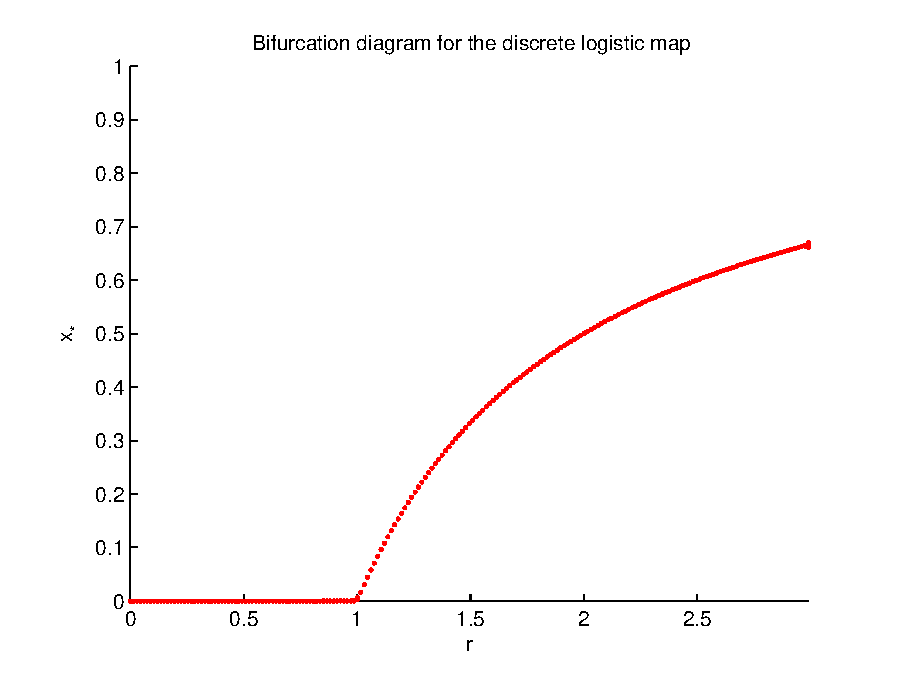
\includegraphics[width=0.5\textwidth]
{../figs_02_population_growth/bif_cascade_1}
\end{center}

\vskip0.5cm
\noindent{\bf Conclusion 2.} Building upon {\bf Conclusion 1}, we therefore deduce that
\begin{itemize}
\item if $r\in(0,1)$, then $x=0$ is attracting, and the fixed point $x=p$ does not exist,
\item if $r\in(1,3)$, then $x=0$ is repelling, and the fixed point $x=p$ exists and is attracting,
\item if $r>3$, then $x=0$ is repelling, and the fixed point $x=p$ exists and is repelling.
\end{itemize}


\begin{remark}
A fixed point that is such that $|f'(p)|\neq 1$, or a periodic point such that $|(f^k)'(p)|\neq 1$, is called \emph{hyperbolic}. In the case that $|f'(p)|=1$, or, for a periodic point, $|(f^k)'(p)|=1$, then $p$ is called \emph{non hyperbolic}. The non hyperbolic case is harder to treat. Here, the case $r=1$ is a \emph{non hyperbolic} case. However, the probability that $r=1$ is zero (the set $r=\{1\}$ has measure zero in the parameter domain $0<r<4$), explaining why, most of the time, the case of $r$ taking a single value, such as $r=1$, is omitted.
\end{remark}



\subsection{Stable sets of the fixed points}
{\bf Conclusion 2} establishes that $x=0$ and $x=p$ are attracting when, respectively, $r\in(0,1)$ and $r\in(1,3)$. This is not sufficient to characterize the behavior of all solutions. Remember that attractiveness of a fixed point $x^*$ implies that there is a neighborhood of $x^*$ that belongs to $W^s(x^*)$, i.e., there exists 
a neighborhood $\mathcal{N}\ni x^*$ such that $\forall x\in\mathcal{N}$, $x$ is forward asymptotic to $x^*$.

If we want to make sure that we have the ``complete picture'', we need to show that $W^s(x^*)=[0,1]$, i.e., that all solutions go to $x^*$. There are several ways to tackle this problem, only one is shown here.

\subsubsection{Case of the fixed point $x=0$ (i.e., case $0<r<1$)}
Since $r<1$, it follows that $f_r(x)=r x(1-x)<x(1-x)$ Also, $x\in[0,1]$ implies that $1-x\in[0,1]$, and therefore $f_r(x)<x(1-x)\leq x$. Therefore, for any $x_0\in[0,1]$,
\begin{align*}
x_1 &= f_r(x_0) \\
&< x_0 \\
x_2 &= f_r(x_1) \\
& < x_1.
\end{align*}
Therefore we have a strictly decreasing sequence. Since $[0,1]$ is invariant, the sequence is bounded below by $0$. Therefore $\lim_{k\to\infty}f^k(x_0)=0$, and $W^s(0)=[0,1]$ when $0<r<1$. Therefore we can strengthen {\bf Conclusion 2}.

\noindent{\bf Conclusion 3$'$.} If $0<r<1$, then for all $x_0\in[0,1]$, $\lim_{k\to\infty}f^k(x_0)=0$, or, equivalently, $\lim_{t\to\infty}x_t=0$.

\begin{remark}
In the considerations above, we could have used Theorem~\ref{th:gas_1} directly, once it was established that $f_r(x)<x$.
\end{remark}
 

\subsubsection{Case of the fixed point $x=p$ (i.e., case $1<r<3$)}
We know that $f_r$ is increasing from a minimum of 0 at $x=0$ to a maximum $r/4$ at $x=1/2$, and then decreasing from there to a minimum of 0 at $x=1$. Therefore, we must distinguish two cases: $r<2$ and $r>2$.


\paragraph{Case $1<r<2$}
In the case $r<2$, the intersection of $f_r(x)$ with the first bisectrix $x$ occurs before the maximum $r/4$ is reached (see Figure~\ref{fig:logistic_1dot5}).
\begin{figure}[htbp]
\begin{center}
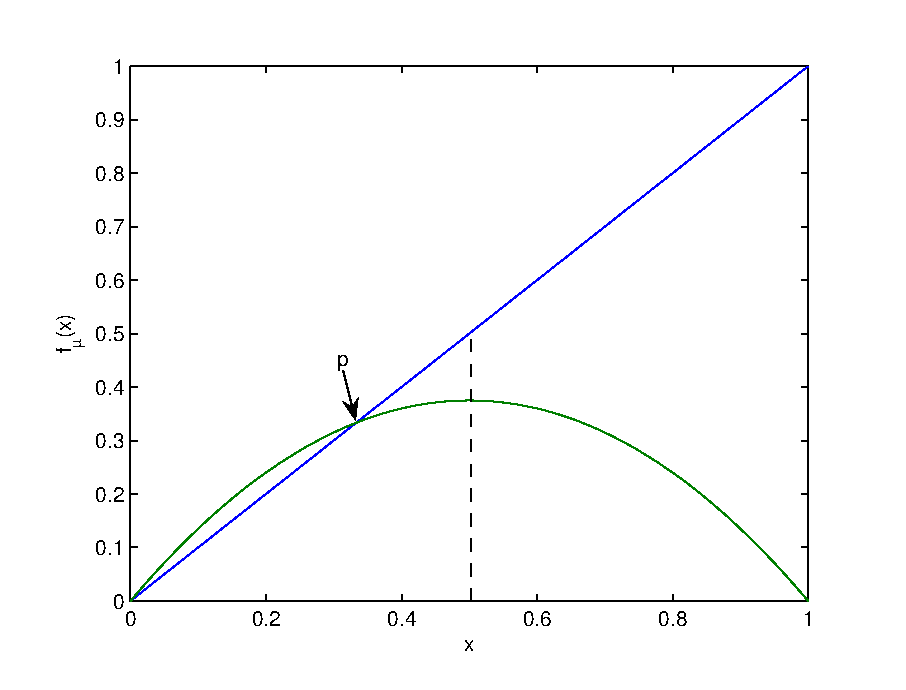
\includegraphics[width=0.5\textwidth]{../figs_02_population_growth/logistic_1dot5}
\end{center}
\caption{The function $f_{1.5}(x)$.}\label{fig:logistic_1dot5}
\end{figure}
Then we are in a position to use part {\bf a} in Theorem~\ref{th:FP_gas_discrete_4}, giving the conclusion.

\paragraph{Case $2<r<3$}
In the case $r>2$, the intersection of $f_r(x)$ with the first bisectrix $x$ occurs after the maximum $r/4$ is reached (see Figure~\ref{fig:logistic_2dot5}).
\begin{figure}[htbp]
\begin{center}
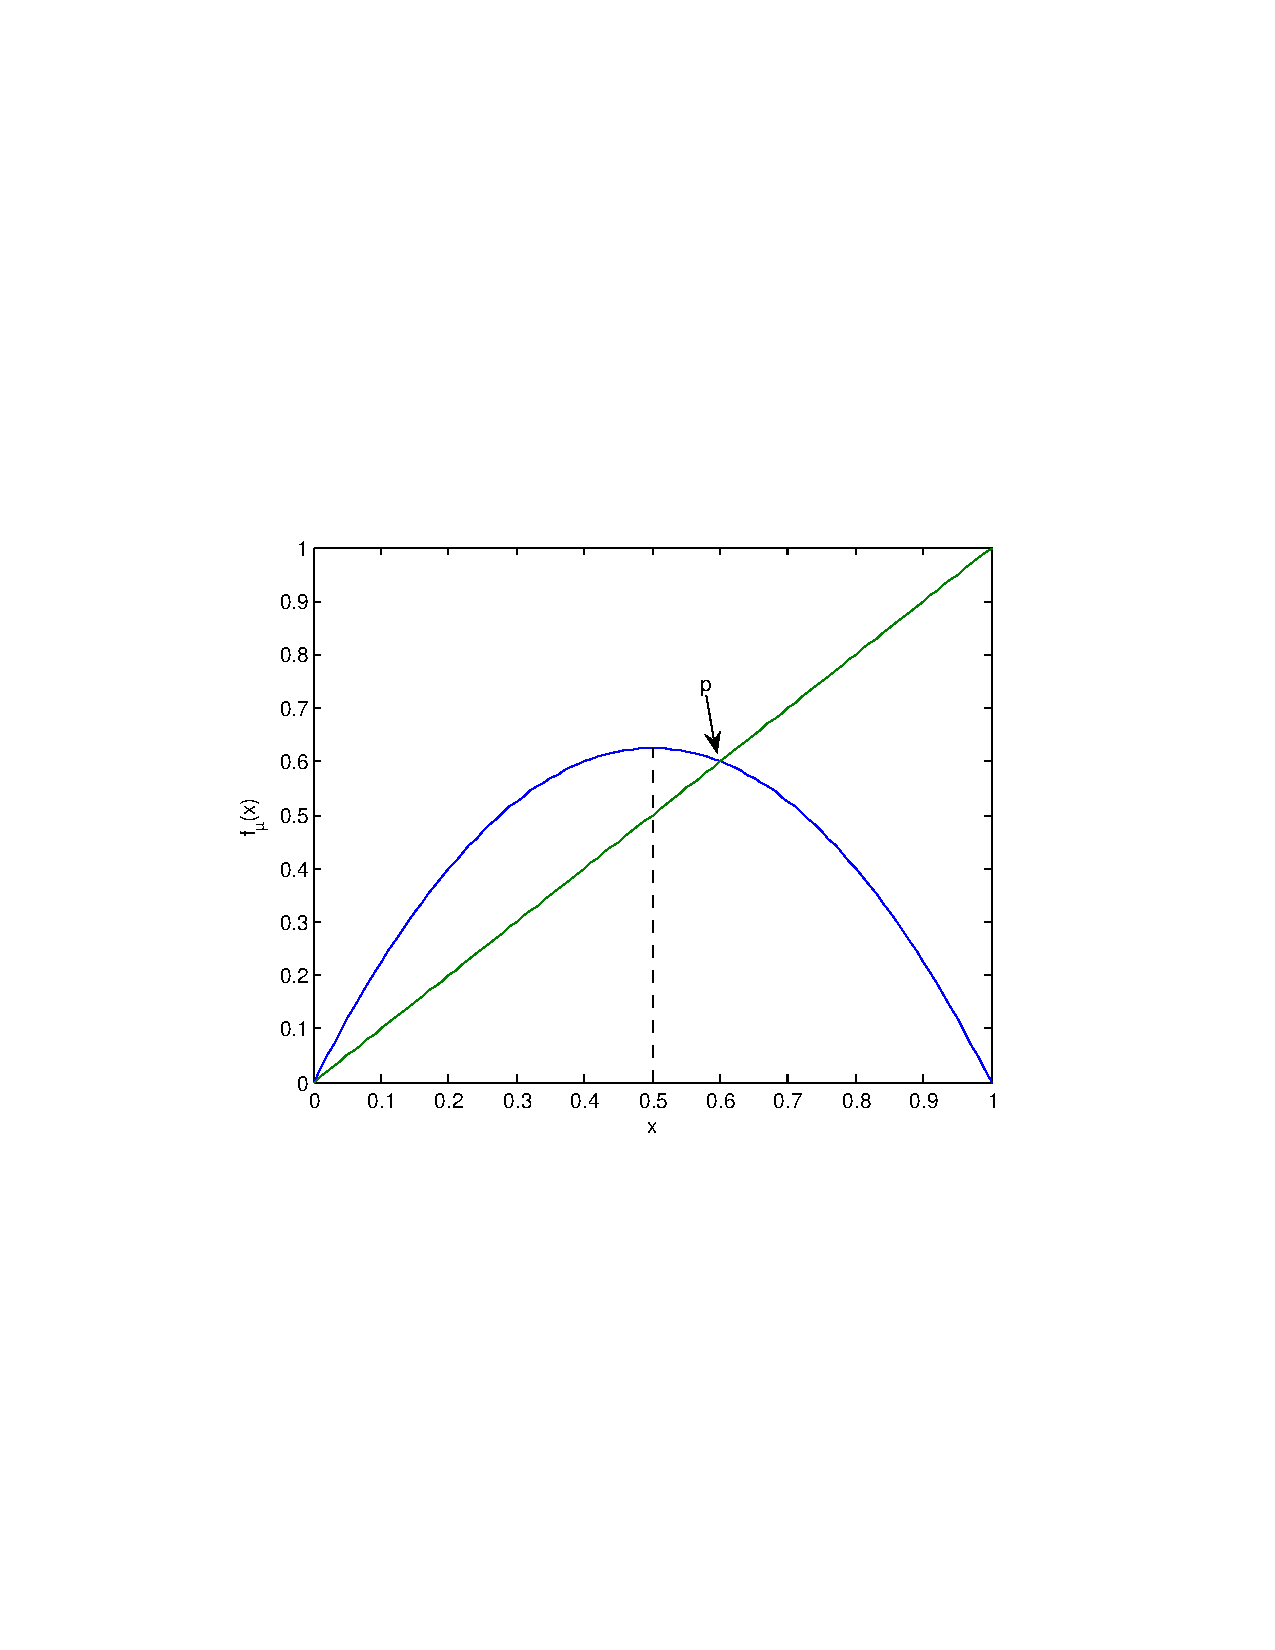
\includegraphics[width=0.5\textwidth]{../figs_02_population_growth/logistic_2dot5}
\end{center}
\caption{The function $f_{2.5}(x)$.}\label{fig:logistic_2dot5}
\end{figure}
We use Theorem~\ref{th:gas_2} in Appendix~\ref{sec:global_stability}. In order to be able to apply this theorem, we must first prove that there are no 2-cycles. For this purpose, we could try to use Theorem~\ref{th:no_cycles}, but it fails to provide the conclusion here. Here, we can use the result from Section~\ref{sec:2cycles}, where it is shown by explicit calculation that there are no 2-cycles for $r<3$.
It is clear that $f$ satisfies the hypotheses of Theorem~\ref{th:gas_2}. Indeed, $f$ is decreasing for $x>1/2$.

\begin{remark}
We could also have used part {\bf b} in Theorem~\ref{th:FP_gas_discrete_4}, but this required to show that $f^2(x)>x$ for $x\in(1/2,p)$.
\end{remark}

{\bf Global stability}
By theorem \ref{th:FP_gas_discrete_4} the equilibrium $p$ is globally asymptotically stable for $1<\mu<3$.


\paragraph{Case $r=2$}
The result used to treat the case $r<2$ can, in the present case, be extended to include the case where $r=2$.


% Here, the first idea would be to show the following:
% \begin{itemize}
% \item if $x_0\in(0,p)$, then $\{x_k\}$ is an increasing sequence,
% \item if $x_0\in(p,1)$, then $\{x_k\}$ is a decreasing sequence.
% \end{itemize}
% Note, however, that this is not sufficient: clearly, nothing forbids the sequence from ``jumping'' from one side of $p$ to the other. This is easy to see using cobwebbing: choosing $x_0$ such that $f_\mu(x_0)>p$ is not difficult (if suffices to choose $x_0$ such that $f_\mu(x_0)$ is above the line $y=p$). We thus want to show that the jumps take us closer and closer to $p$.
% 
% To do this, we consider the interval $I_0=(\varepsilon,1)$, with $\varepsilon>0$ small. We have $f_\mu'(0)=\mu>1$, and by continuity of $f_\mu'$, it is therefore possible to choose $\varepsilon$ small enough that $f_\mu'(\varepsilon)=\mu(1-2\varepsilon)>1$.



\subsection{Existence of points of period 2}
\label{sec:2cycles}
We now study the existence of periodic points with least period 2, that is, fixed points of the map $f_r^2(x)$. We have
\begin{align}
f_r^2(x) &= f_r(f_r(x)) \nonumber\\
&= r f_r(x)(1-f_r(x)) \nonumber\\
&= r^2 x(1-x)(1-r x(1-x)). \label{eq:f_mu_2_a}
\end{align}
Remark that 0 and $p$ are points of period 2. Indeed, a fixed point $x^*$ of $f$ satisfies $f(x^*)=x^*$, and as a consequence, $f^2(x^*)=f(f(x^*))=f(x^*)=x^*$. This is extremely helpful in localizing the other periodic points, if there are any. Indeed, writing the fixed point equation as
\[
f_r^2(x)-x=0,
\]
and defining $Q(x):=f_r^2(x)-x$, we see that, since $0$ and $p$ are fixed points of $f_r^2$, they are roots of $Q(x)$. Therefore, $Q$ can be factorized as
\[
Q(x)=x(x-p)(-r^3x^2+Bx+C),
\]
since it is clear from \eqref{eq:f_mu_2_a} that $f_r^2$ is a polynomial of degree 4 with leading coefficient equal to $-r^3$. Substituting the value $(r-1)/r$ for $p$ in $Q$, developing $Q$ and \eqref{eq:f_mu_2_a} and equating coefficients of like powers gives
\begin{equation}\label{eq:Q}
Q(x)=x\left(x-\frac{r-1}{r}\right)\left(-r^3 x^2+r^2(r+1)x-r(r+1)\right).
\end{equation}
The roots of \eqref{eq:Q} are the fixed points of $f_r^2$. Since $x=0$ and $x=p$ are already known, we can concentrate on the roots of the polynomial
\[
R(x):=-r^3 x^2+r^2(r+1)x-r(r+1).
\]
The discriminant is $\Delta=r^4(r+1)^2-4r^4(r+1)=r^4(r+1)(r+1-4)=r^4(r+1)(r-3)$. Therefore, $R$ has no real root if $r<3$, a double real root if $r=3$ and distinct real roots if $r>3$. We want real valued solutions, so discard the case $r<3$. In the case $r=3$, the root is
\[
\left.\frac{r+1}{2r}\right|_{r=3}=\frac 23,
\]
which is the value of $p$ when evaluated at $r=3$: the fixed point $p$ and the fixed point deduced from $R$ coincide at $r=3$.

So we now consider the case $r>3$. In this case, $R$ has two distinct real roots (that is, $f_r^2$ has two distinct real fixed points) given by
\[
\bar x_{1,2}=\frac{r+1\pm\sqrt{(r+1)(r-3)}}{2r}.
\] 
First, remark that for $r>3$ but very close to 3, it follows from the continuity of $R$ that the roots are very close to the double root $2/3$, and hence are in $(0,1)$.
More than the actual value of the roots, what is of interest at this point is to determine whether they remain in $(0,1)$ for all values of $3<r<4$.
If a root is not in $(0,1)$, it is considered to be non biologically relevant and therefore is ignored.

To show that the roots remain in $(0,1)$ as we move away from 3, we could proceed directly using the expression for $\bar x_{1,2}$. Instead, we use Descartes' rule of signs (Theorem~\ref{th:descartes}, Appendix~\ref{sec:descartes}). For this, remark that $R$ has signed coefficients $-+-$, giving two sign changes and the possibility of 0 or 2 positive real roots. On the other hand, $R(-x)$ has signed coefficients $---$, hence there are no negative real roots. As we are in the case where the roots are real, it follows that both roots are positive.

To show that the roots are also smaller than 1, consider the change of variables $z=x-1$. The polynomial $R$ is transformed into 
\begin{align*}
R_2(z) &= -r^3 (z+1)^2+r^2(r+1)(z+1)-r(r+1) \\
&= -r^3z^2+r^2(1-r)z-r.
\end{align*}
For $r>1$, all the coefficients of this polynomial are negative, implying that $R_2$ has no root $z>0$, implying in turn that $R$ has no root $x>1$.
\begin{figure}[htbp]
\begin{center}
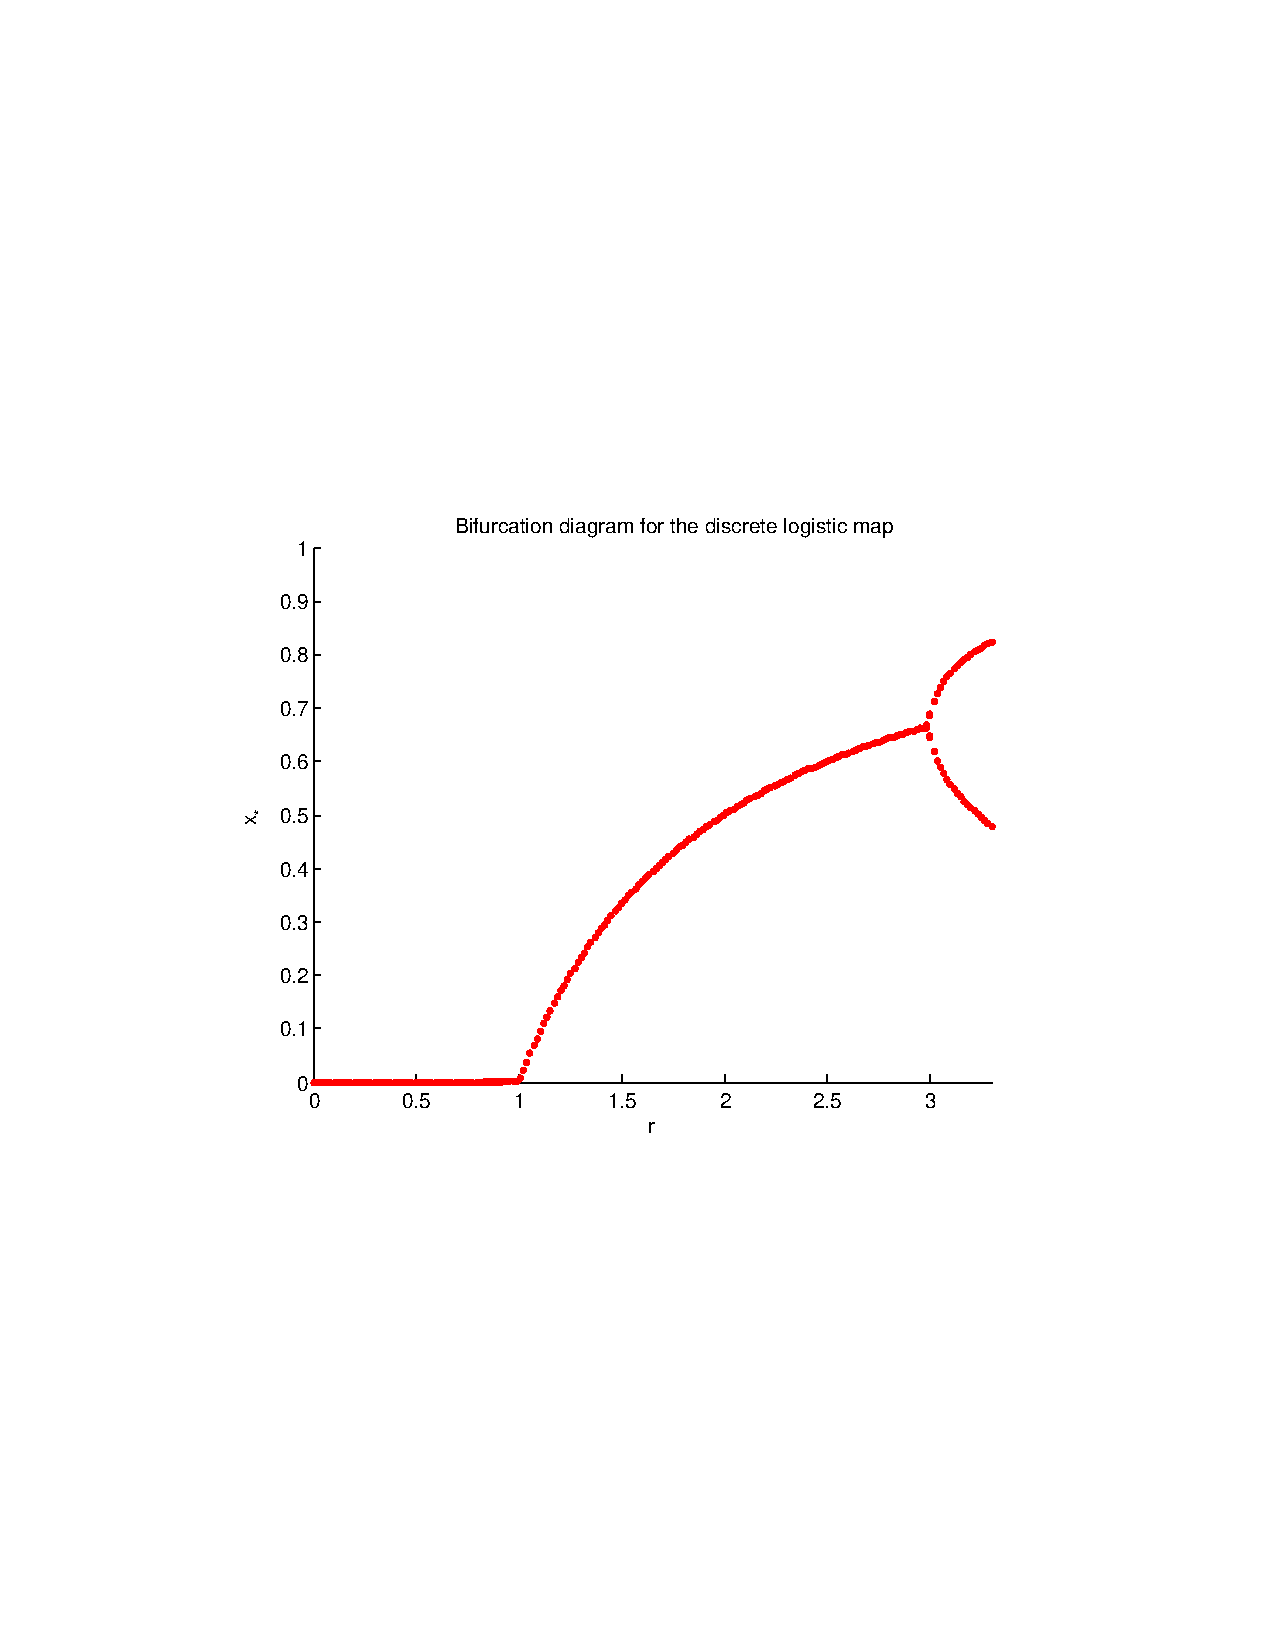
\includegraphics[width=0.5\textwidth]
{../figs_02_population_growth/bif_cascade_3}
\caption{Bifurcation diagram for the discrete logistic map showing the birth of the fixed point at $r=1$ and of the 2-cycle at $r=3$.}
\end{center}
\end{figure}


\subsection{Attractiveness of the periodic orbit}
We use Theorem~\ref{th:} which states that the $2-$cycle is locally asymptotically stable if
\[
|f_r'(\bar x_1)f_r'(\bar x_2)|<1.
\]
From \eqref{eq:dlogistic_map}, we obtain
\begin{align*}
|f_r'(\bar x_1)f_r'(\bar x_2)|
&=\left|
\left(r-(r+1)+\sqrt{(r+1)(r-3)}\right)
\left(r-(r+1)-\sqrt{(r+1)(r-3)}\right)
\right| \\
&=\left|
\left(1+\sqrt{(r+1)(r-3)}\right)
\left(1-\sqrt{(r+1)(r-3)}\right)
\right|.
\end{align*}
Therefore,
\begin{align*}
|f_r'(\bar x_1)f_r'(\bar x_2)|<1 &\Leftrightarrow |1-(r+1)(r-3)|<1 \\
&\Leftrightarrow -1<1-(r+1)(r-3)<1 \\
&\Leftrightarrow 0<(r+1)(r-3)<2.
\end{align*}
Evidently, the inequality $0<(r+1)(r-3)$ is satisfied if $r>3$. On the other hand, the quadratic inequality $(r+1)(r-3)<2$ is satisfied if $r<1+\sqrt{6}$.
Therefore, the 2-cycle is locally asymptotically stable if 
\[
3<r<1+\sqrt{6}
\]
and unstable if $r>1+\sqrt{6}$.






\subsection{The cascade of bifurcation to chaos}
\label{sec:chaos}
We have seen that at $r=1$, $r=3$ and $r=1+\sqrt{6}$, there are changes in the stability of the various equilibria that are present, and that additional equilibria can be born. These values of $r$ are called \textbf{bifurcation points}. 

The first bifurcation that occurs, at $r=1$, is different in nature from the ones that follow. It is called a \textbf{transcritical bifurcation}, and corresponds to an exchange of stability between zero and $p$ (recall that although $p$ is not relevant for $r<1$, it still does exist). 

Subsequent bifurcations are called \textbf{period-doubling bifurcations}. By continuing the analysis of the logistic map, we see that it undergoes a a sequence of period doubling bifurcations, called the \textbf{period-doubling cascade}, as $r$ increases from 3 to 4 (see Figure~\ref{fig:bif_cascade_29_4}):
\begin{itemize}
\item for $1+\sqrt{6}<r<3.5441$ there is a stable $4-$cycle, followed by a period doubling at $r=3.5441$;
\item for $3.5441<r<3.5644$ there is a stable $8-$cycle, followed by a period doubling at $r=3.5644$;
\item for $3.5644<r<3.5688$ there is a stable $16-$cycle, followed by a period doubling at $r = 3.5688$;
\item $\ldots$ other stable cycles of increasing period $2^n$;
\item finally, for $r> 3.57$, a cycle of period $3$ exists. In that case, the solutions are called \textbf{chaotic} (see below).
\end{itemize}
\begin{figure}[htbp]
\begin{center}
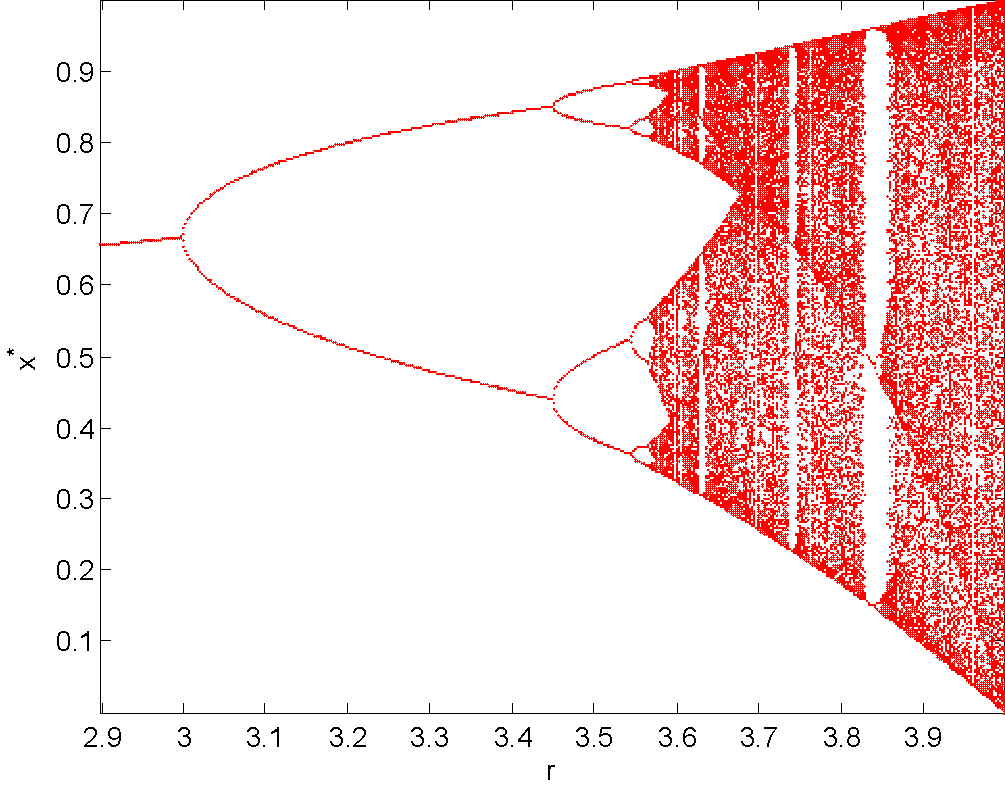
\includegraphics[width=0.6\textwidth]
{../figs_02_population_growth/cascade_29_4}
\caption{Bifurcation cascade for $2.9\leq r\leq 4$.}
\label{fig:bif_cascade_29_4}
\end{center}
\end{figure}
The points at which the period doublings occur has a very interesting (and intriguing) property:
The bifurcation points form a sequence, $\{r_n\}$, that has the property that
\[
\lim_{n\to\infty}\frac{r_n-r_{n-1}}{r_{n+1}-r_n}
\]
exists and is a constant, called the Feigenbaum constant, equal to 4.669202\ldots
This constant has been shown to be the same in many of the maps that undergo the same type of cascade of period doubling bifurcations.

To finish, let us briefly discuss chaos. Note that the mathematics are quite involved and well beyond the scope of these notes.
Denoting $\triangleright$ an order symbol, Sharkovskii's ordering of integers is as follows:
\begin{gather*}
3\triangleright 5\triangleright 7 \triangleright 9 \triangleright 11\triangleright \cdots \triangleright 2\cdot 3\triangleright  2\cdot 5\triangleright \cdots \triangleright 2\cdot 9\triangleright\cdots\triangleright 2^2\cdot 3\triangleright 2^2\cdot 5\triangleright \cdots \\
\triangleright 2^n\cdot 3\triangleright 2^n\cdot 5\triangleright \cdots\triangleright 2^{n+1}\cdot 3\triangleright 2^{n+1}\cdot 5\triangleright \cdots
\triangleright 2^{n+1}\triangleright 2^n\triangleright \cdots 2^2 \triangleright 2\triangleright 1.
\end{gather*}
This gives an ordering of all positive integers. The following result helps characterizing the behavior of the cascade.
\begin{theorem}[Sharkovskii]\label{th:sharkovskii}
Let $f:I\subset\IR\to\IR$ be a continuous function. Assume that $f$ has a point of least period $n$ and $n\triangleright k$. Then $f$ has a point of least period $k$.
\end{theorem}


\begin{figure}[htbp]
\begin{center}
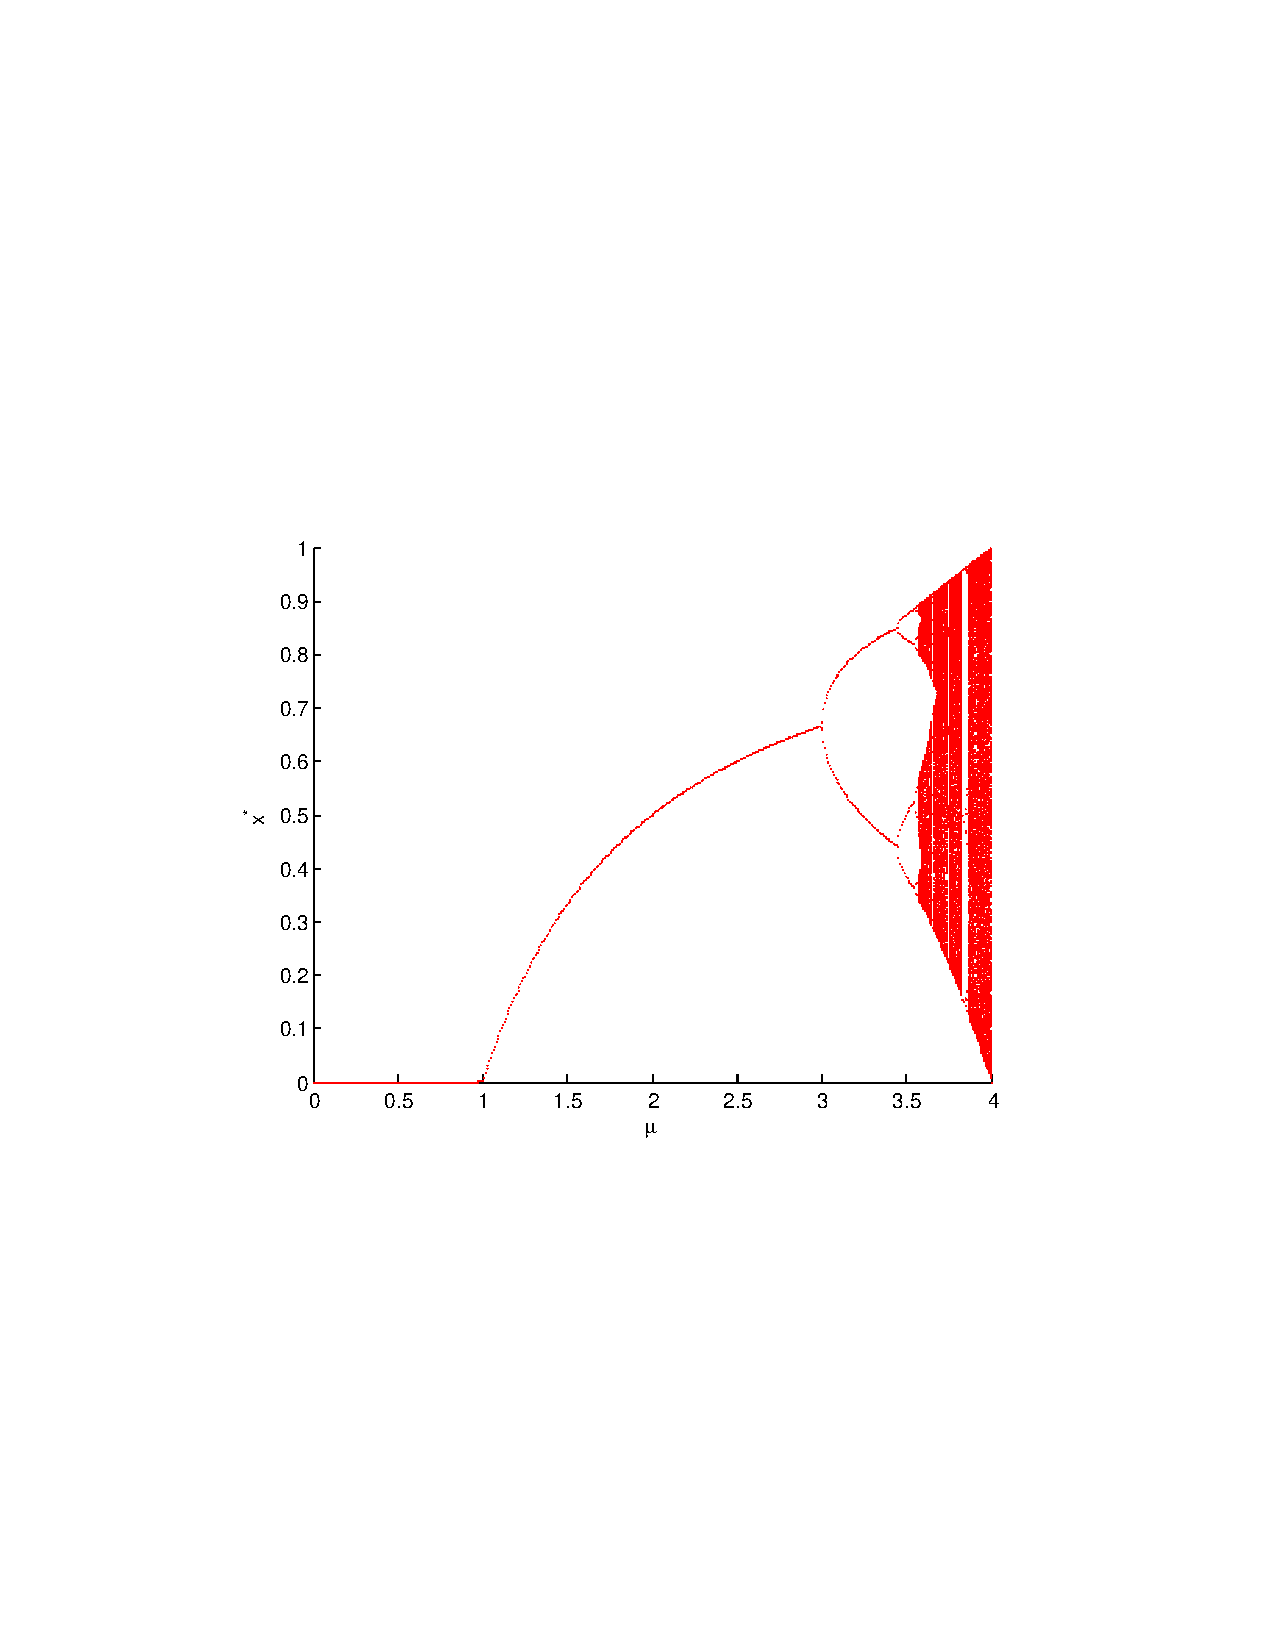
\includegraphics[width=0.5\textwidth]
{../figs_02_population_growth/analysis_logistic_cascade_full}
\end{center}
\caption{The cascade of bifurcation to chaos for the logistic map.}
\end{figure}

We have seen that for $r>3.57$, there is a cycle of period 3 for the logistic map. By Sarkovskii's theorem, the presence of period 3 points implies the presence of points of all periods.
At this point, the system is said to be in a \textbf{chaotic regime}, or \textbf{chaotic}.




\section{Conclusion}

We have used three different modelling paradigms to describe the growth of a population in a \textbf{logistic} framework:
\begin{itemize}
\item The ODE version of Section~\ref{sec:ODE_logistic} has monotone solutions converging to the carrying capacity $K$.
\item The DDE version of Section~\ref{sec:DDE_logistic} has oscillatory solutions, either converging to $K$ or, if the delay is too large, periodic about $K$.
\item The discrete time version of Section~\ref{sec:DE_logistic} has all sorts of behaviors, and can be chaotic.
\end{itemize}
It is important to be aware that the {\bf choice of modelling method} is almost {\bf as important} in the outcome of the model as the precise formulation/hypotheses of the {\bf model}.


%\section{Critic of the logistic equation in the US census case}
%
%\frame{\frametitle{What is wrong with the logistic equation here?}
%\begin{itemize}
%\item The carrying capacity is constant.
%\item The model does not take immigration into account (for the US, this is an important component).
%\end{itemize}
%}
%
%
%\section{Population curves -- Gompertz}
%
%\frame{
%\begin{center}
%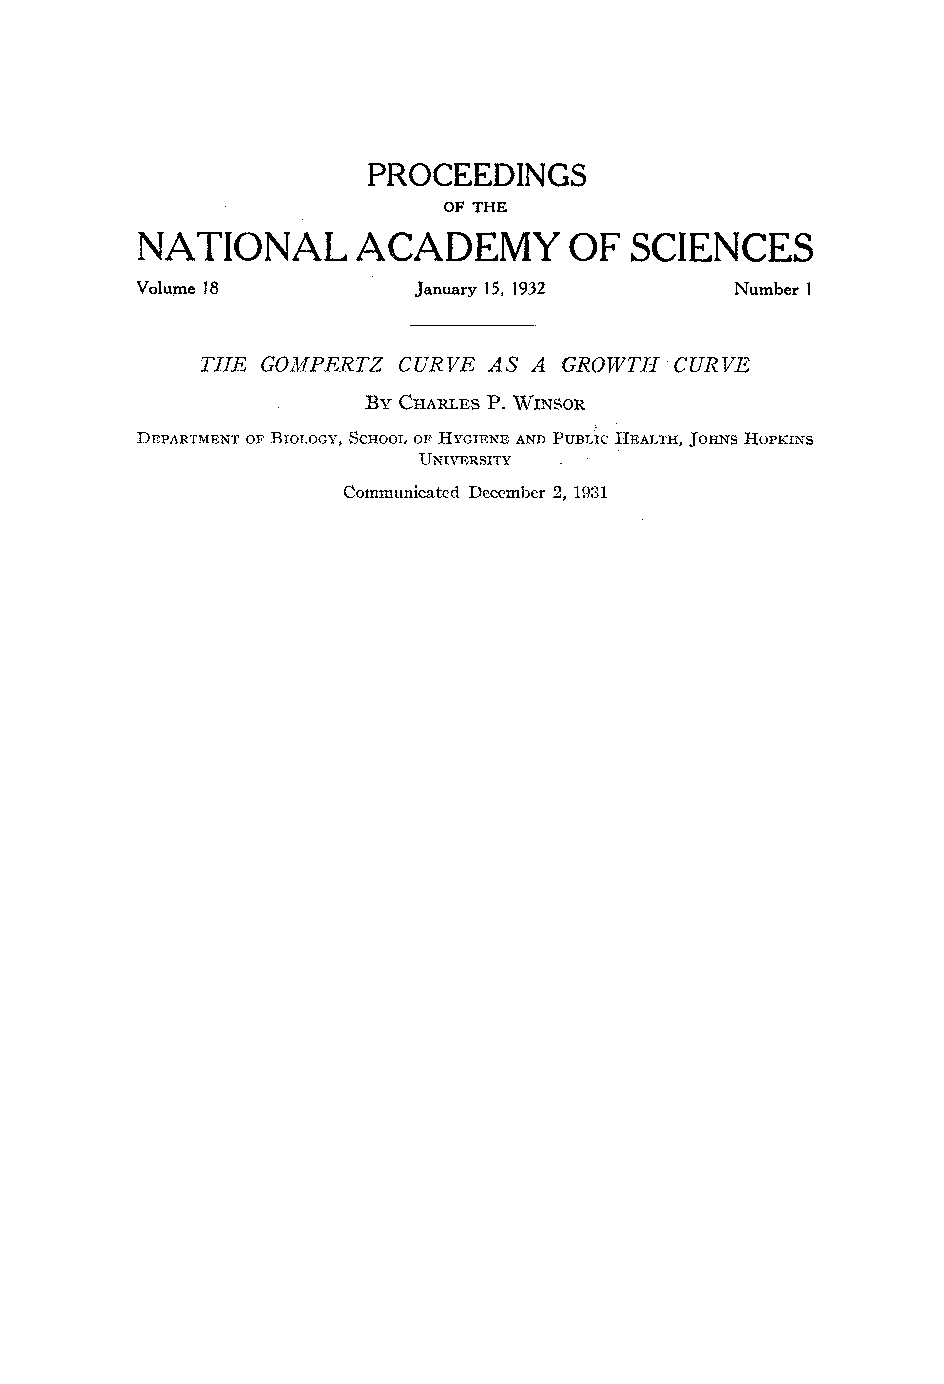
\includegraphics[width=0.95\textwidth]{title_Winsor1932PNAS18}
%\end{center}
%}
%
%\frame{
%\begin{center}
%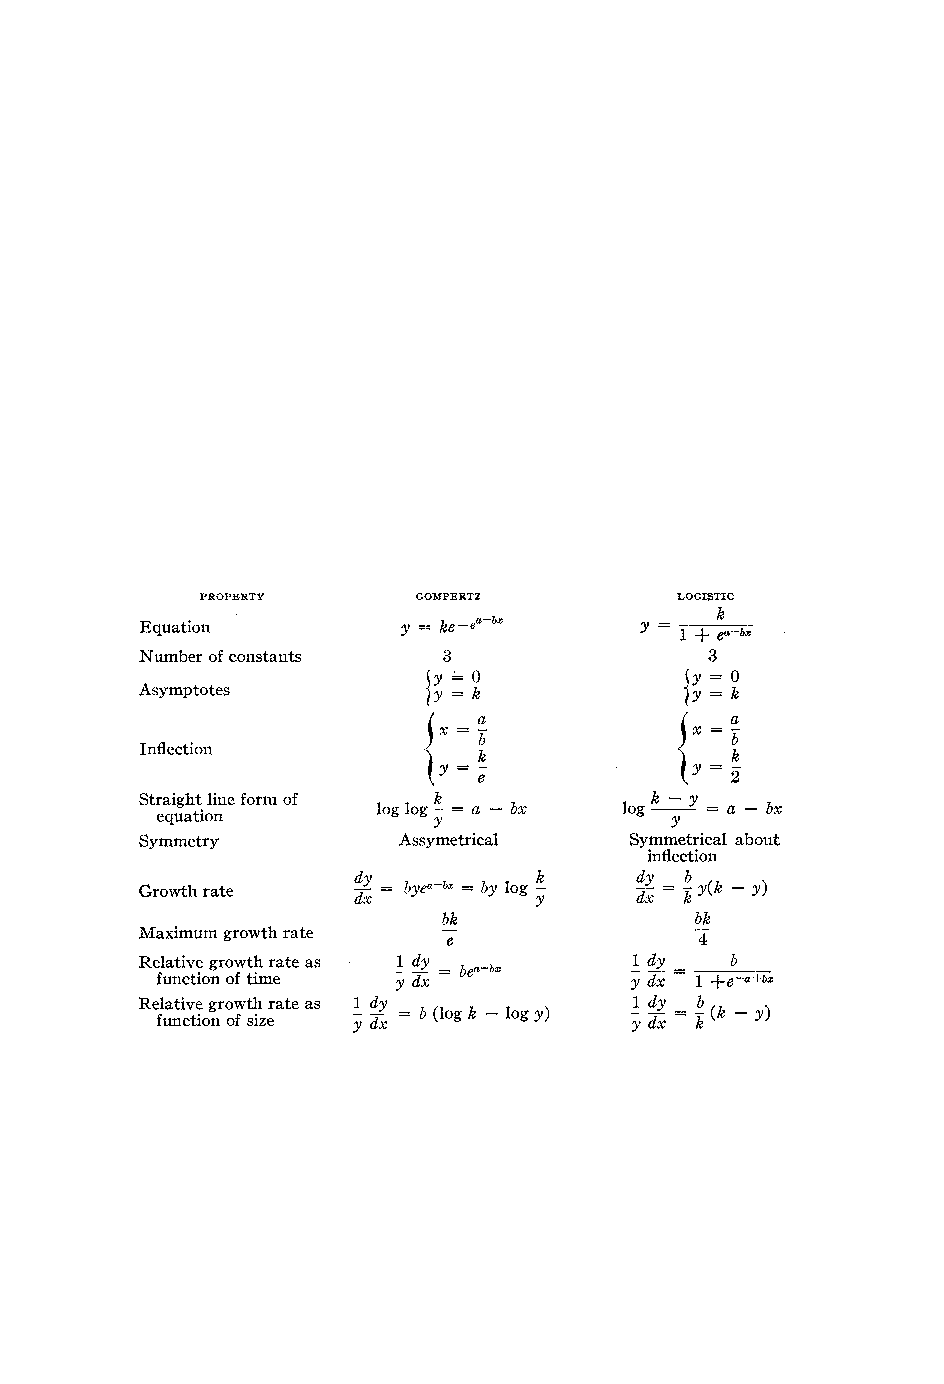
\includegraphics[width=0.95\textwidth]{table_Winsor1932PNAS18}
%\end{center}
%}
%

\chapter[Residence time]{Time of residence in states\\[0.5cm] Introduction to
compartmental models}
\label{chap:residence_time}


\section{Time spent in a state -- Some probability theory}
\label{sec:residence_time}
We suppose that a system/object/individual can be in two states $S_1$ and $S_2$.
These states can be anything:
\begin{itemize}
\item $S_1$: working, $S_2$: broken,
\item $S_1$: infected, $S_2$: recovered,
\item $S_1$: alive, $S_2$: dead.
\end{itemize}
At time $t=0$, the system is in state $S_1$.
An event happens at some time $t=\tau\geq 0$, which triggers the switch from state $S_1$ to state $S_2$. Suppose that we are able to conduct an experiment with infinitely many copies of this system, and are interested in obtaining some type of description of the time it takes for the system to switch states.

Let us reformulate this problem in the language of probability theory.
A \textbf{random variable} is a variable that takes random values, that is, a mapping from random experiments to numbers. 
Here, let us call $T$ the random variable ``time spent in state $S_1$ before switching into state $S_2$''. 
We take a collection of objects or individuals that are in state $S_1$ and want some law for the \textbf{distribution} of the times spent in $S_1$, i.e., a law for $T$.
For example, we make light bulbs and would like to tell our customers that on average, our light bulbs last 200 years.
For this, we conduct an \textbf{infinite} number of experiments, and observe the time that it takes, in every experiment, to switch between $S_1$ and $S_2$.
From this, we deduce a model, which in this context is called a \textbf{probability distribution}.

Before we proceed any further, let us make one remark here. Roughly speaking, probability theory assumes that it is indeed possible to carry out an infinite number of experiments. Statistics, on the other hand, deals with the use of probability theory in ``real life'', where the number of experiments is intrinsically limited.

\begin{figure}[htbp]
\begin{center}
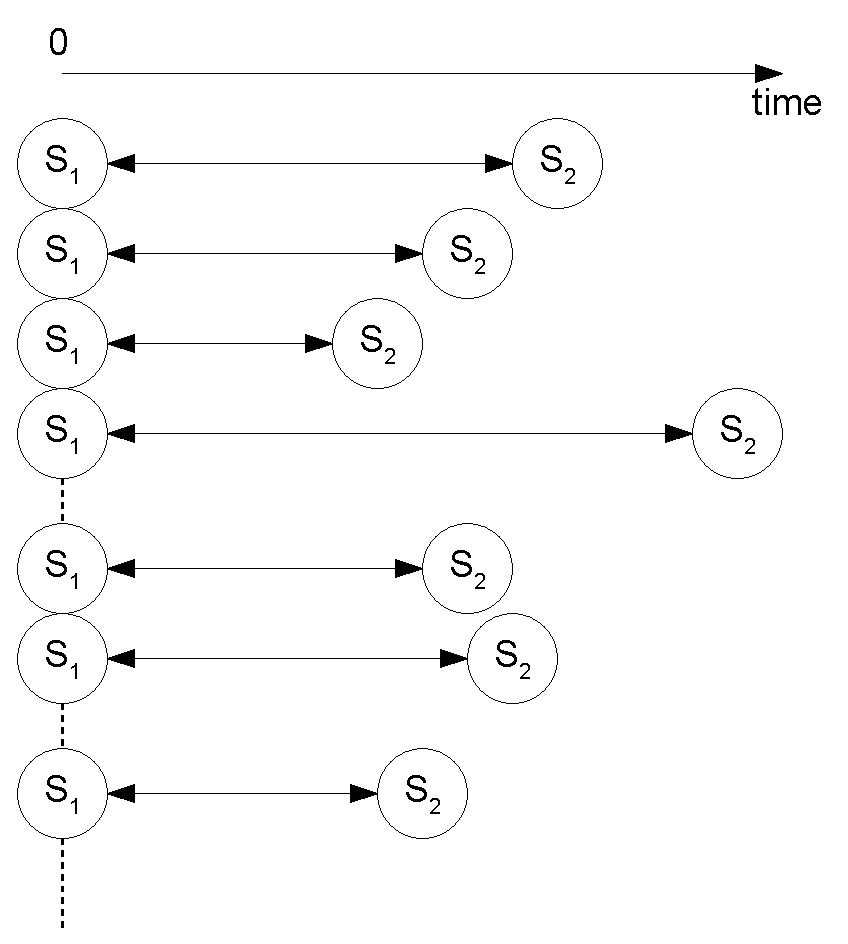
\includegraphics[height=0.45\textwidth]
{../figs_03_residence_time/random_length_sample}
\caption{Time until the switch from state $S_1$ to state $S_2$, for several experiments. From this, we could deduce a distribution for the time of sojourn in state $S_1$.}
\end{center}
\end{figure}

Returning to the time spent in a state, we assume that $T$ is a \textbf{continuous} random variable, that is, $T$ takes continuous values. Examples of continuous random variables are the height or age of a person (if measured very precisely), distances, times, etc.
Another type of random variables are \textbf{discrete} random variables, which take values in a denumerable set: heads or tails on a coin toss, the number rolled on a dice, the height of a person, if expressed rounded without subunits, the age of a person in years (without subunits), etc.

A \textbf{probability} is a function $\mathcal{P}$, from a probability space to $[0,1]$.
Formally: $(\Omega,\mathcal{F},\mathcal{P})$ is a probability space, with $\Omega$ the \textbf{sample} space, $\mathcal{F}$ a $\sigma$-algebra of subsets of $\Omega$ whose elements are the \textbf{events}, and $\mathcal{P}$ a \textbf{measure} from $\mathcal{F}$ to $[0,1]$ such that $\mathcal{P}(E)\geq 0$, $\forall E\subset\Omega$, $\mathcal{P}(\Omega)=1$ and $\mathcal{P}(E_1\cup E_2\cup\cdots)=\sum_i\mathcal{P}(E_i)$.

A probability gives the likelihood of an event occurring, among all the events that are
possible, in that particular setting. For example, 
\[
\Proba{\textrm{getting heads
when tossing a coin}}=1/2
\]
and 
\[
\Proba{\textrm{getting tails when tossing a
coin}}=1/2.
\]
Since $T$ is continuous, it has a continuous \textbf{probability density function} (p.d.f.), $f$, which satisfies:
\begin{itemize}
\item $f\geq 0$,
\item $\int_{-\infty}^{+\infty}f(s)ds=1$.
\item $\Proba{a\leq T\leq b}=\int_a^bf(t)dt$.
\end{itemize}
\begin{figure}[htbp]
\begin{center}
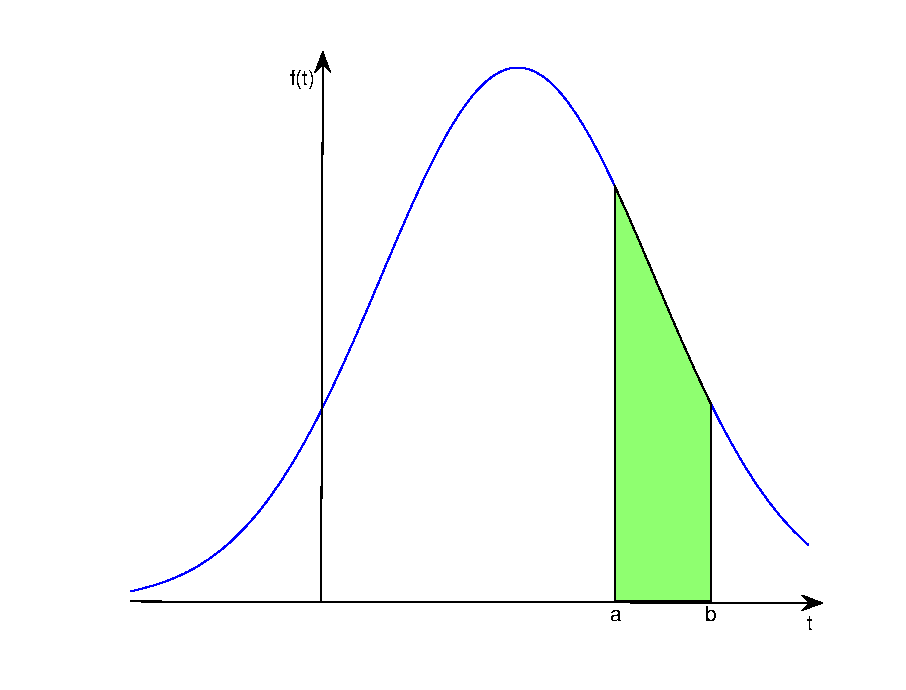
\includegraphics[width=0.5\textwidth]{../figs_03_residence_time/distrib_a_b}
\caption{A continuous probability distribution function (curve) and $\Proba{a\leq T\leq b}$ (area).}
\end{center}
\end{figure}
The \textbf{cumulative distribution function} (c.d.f.) is a function $F(t)$ that characterizes the distribution of $T$, and defined by
\[
F(s)=\Proba{T\leq s}=\int_{-\infty}^sf(x)dx.
\]
\begin{figure}[htbp]
\begin{center}
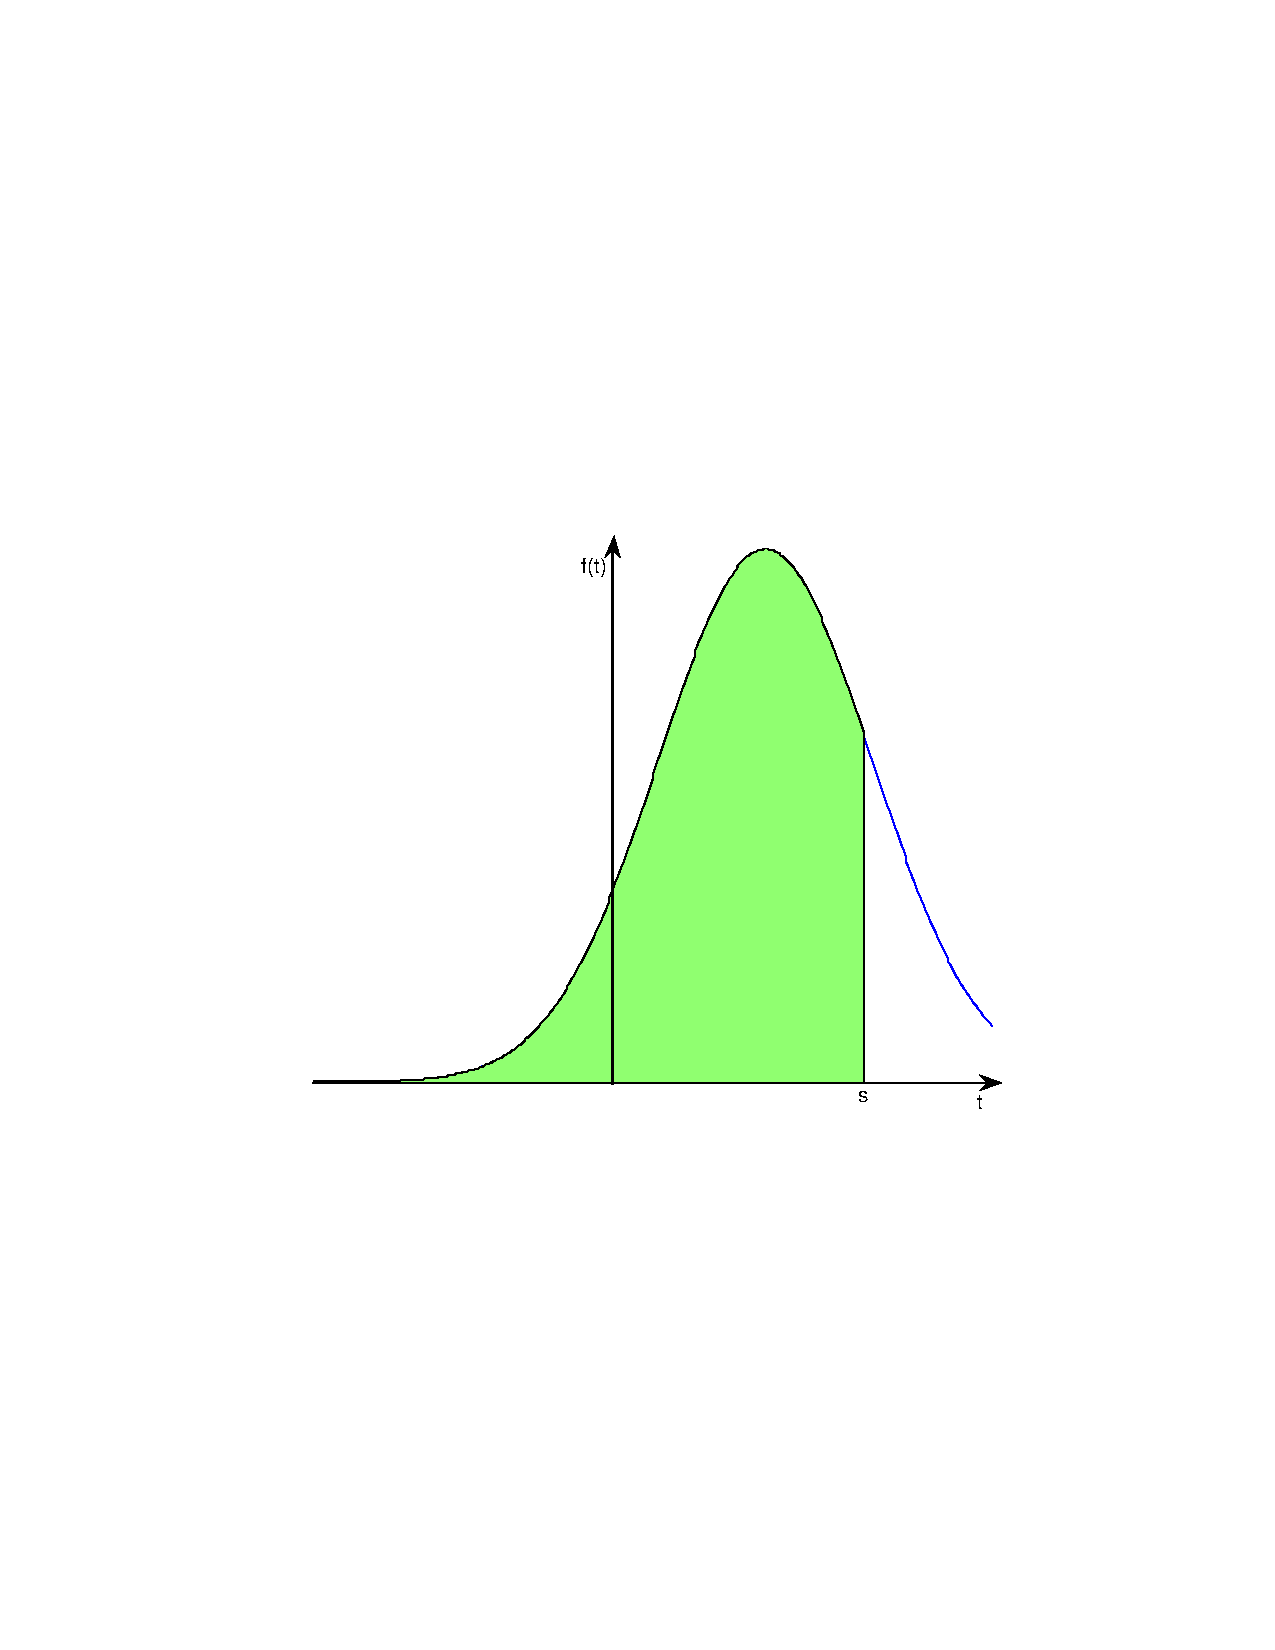
\includegraphics[width=0.45\textwidth]{../figs_03_residence_time/cdf_auc}
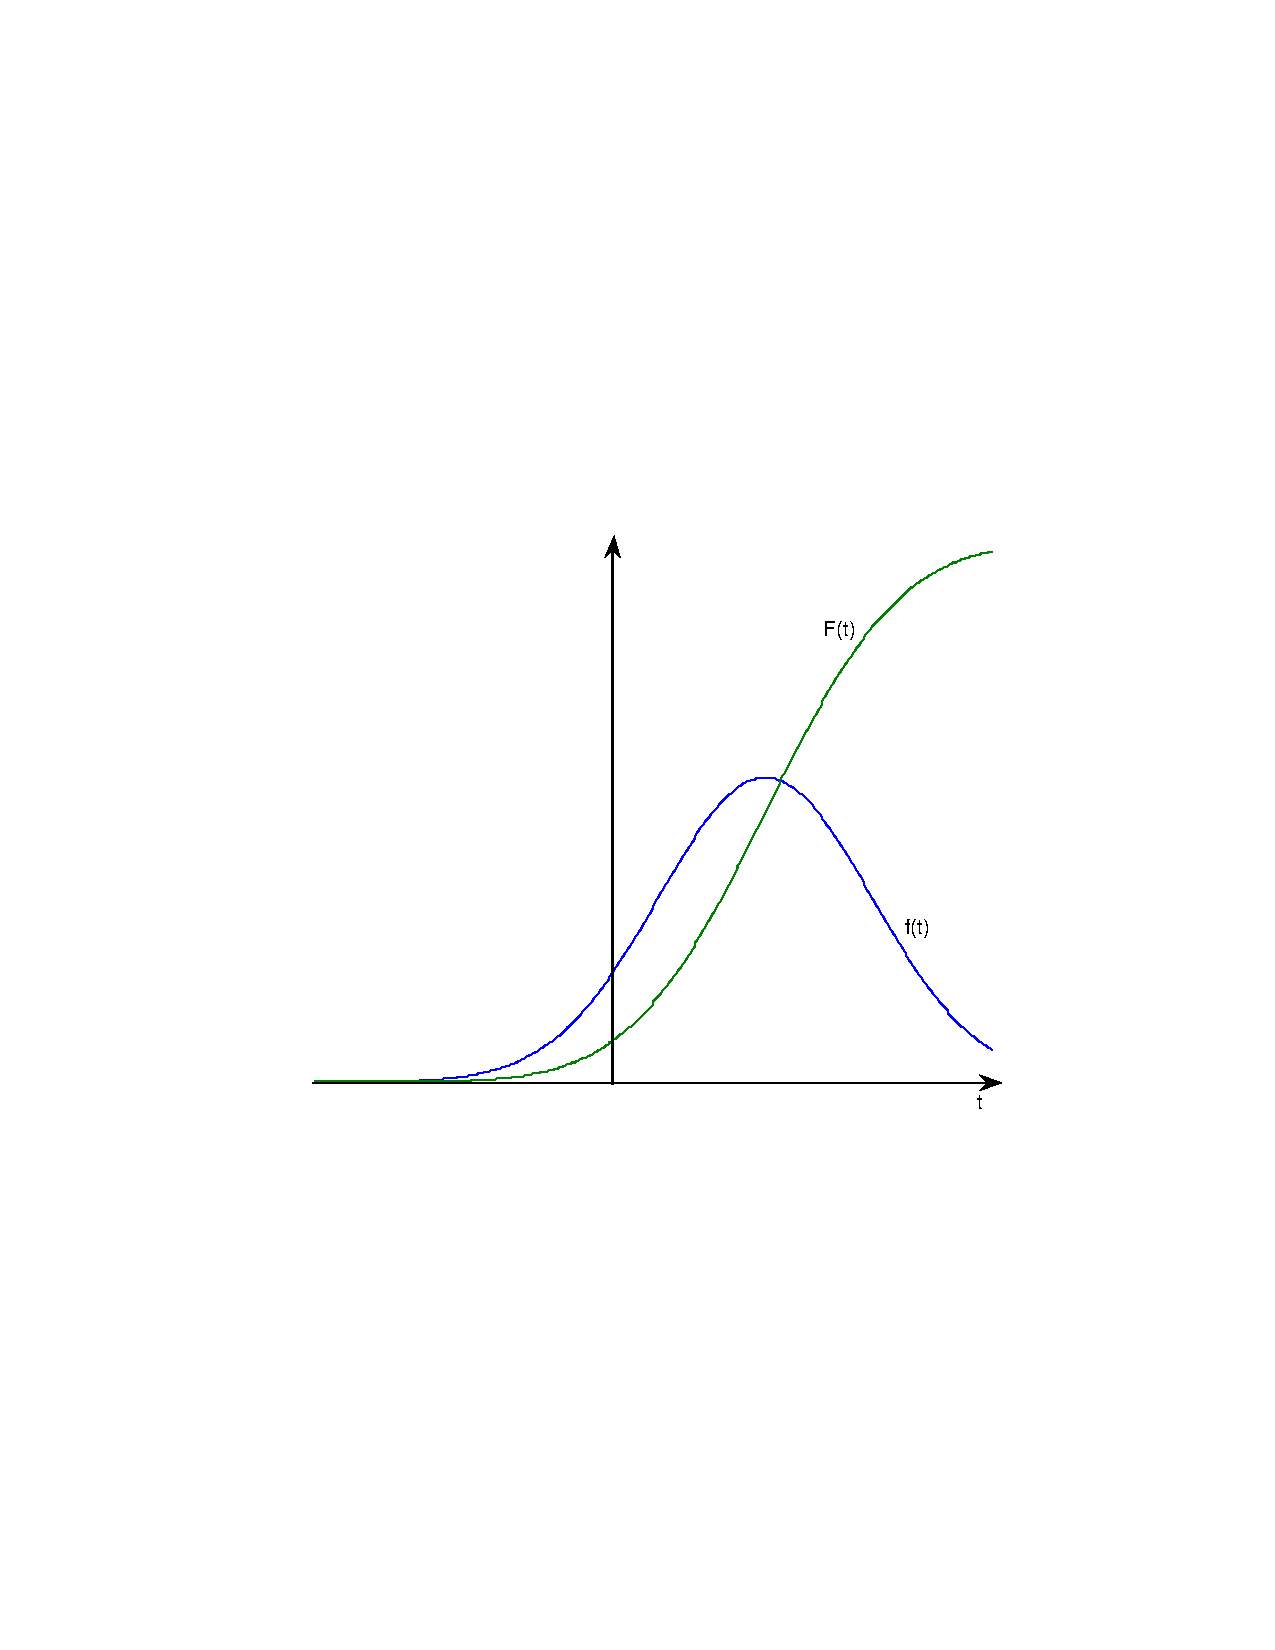
\includegraphics[width=0.45\textwidth]{../figs_03_residence_time/cdf_plot}
\caption{The link between the cumulative distribution function and the probability density function. The integral from $-\infty$ to $t$, shown on the left by the area under the curve $f$, gives a function $F(t)$ (right).}
\label{fig:cum_distrib}
\end{center}
\end{figure}
\begin{itemize}
\item
Since $f$ is a nonnegative function, $F$ is nondecreasing.
\item
Since $f$ is a probability density function, $\int_{-\infty}^{+\infty}f(s)ds=1$, and thus $\lim_{t\to\infty}F(t)=1$.
\end{itemize}
\begin{figure}[htbp]
\begin{center}
\end{center}
\end{figure}

For a continuous random variable $T$ with probability density function $f$, the \textbf{mean} value of $T$, denoted $\bar T$ or $E(T)$, is given by
\[
E(T)=\int_{-\infty}^{+\infty} tf(t)dt.
\]
Another characterization of the distribution of the random variable
$T$ is through the \textbf{survival} (or \textbf{sojourn}) function. 
The survival function of state $S_1$ is given by 
\begin{equation}
  \S(t)=1-F(t)=\Proba{T>t}
  \label{eq:survival}
\end{equation}
This gives a description of the \textbf{sojourn time} of a
system in a particular state (the time spent in the state).
$\S$ is a nonincreasing function (since $\S=1-F$
with $F$ a c.d.f.), and
$\S(0)=1$ (since $T$ is a positive random variable).
The \textbf{average sojourn time} $\tau$ in state $S_1$ is given by
\[
\tau=E(T)=\int_0^\infty tf(t)dt
\]
Assuming that $\lim_{t\to\infty}t\S(t)=0$ (which is verified
for most probability distributions), 
\[
\tau=\int_0^\infty \S(t)dt.
\]



\section{The exponential distribution}

The random variable $T$ has an \textbf{exponential} distribution if its probability density function takes the form
\begin{equation}\label{eq:exp_distrib}
f(t)=\begin{cases}0&\textrm{if }t<0,\\
\theta e^{-\theta t}&\textrm{if }t\geq 0,
\end{cases}
\end{equation}
with $\theta>0$. Then the
survival function for state $S_1$ is of the form $\S(t)=e^{-\theta
  t}$, for $t\geq 0$, and the average sojourn time in state $S_1$ is
\[
\tau=\int_0^\infty e^{-\theta t}dt=\frac 1\theta
\]
If on the other hand, for some constant $\omega>0$,
\[
\S(t)=
\left\{
\begin{array}{ll}
1, & 0\leq t\leq\omega \\
0, & \omega<t
\end{array}
\right.
\]
which means that $T$ has a Dirac delta distribution
$\delta_\omega(t)$, then the average sojourn time is a constant, namely
\[
\tau=\int_0^\omega dt=\omega
\]
These two distributions can be regarded as extremes.



\section{A cohort model} 
We consider a population consisting of individuals born at the same time (a \textbf{cohort}), for example, the same year.
We suppose
\begin{itemize}
\item At time $t=0$, there are initially $N_0>0$ individuals.
\item All causes of death are compounded together. 
\item The time until death, for a given individual, is a random variable $T$, with continuous probability density distribution $f(t)$ and survival function $P(t)$.
\end{itemize}
Denote $N(t)$ the population at time $t\geq 0$. Then
\begin{equation}\label{eq:N_general}
N(t)=N_0P(t).
\end{equation}
\begin{itemize}
\item $N_0P(t)$ gives the proportion of $N_0$, the initial population, that is still alive at time $t$.
\end{itemize}

\paragraph{Case where $T$ is exponentially distributed}
Suppose that $T$ has an exponential distribution with mean $1/d$ (or parameter $d$), $f(t)=de^{-dt}$. Then the survival function is $P(t)=e^{-dt}$, and \eqref{eq:N_general} takes the form
\begin{equation}\label{eq:N}
N(t)=N_0e^{-dt}.
\end{equation}
Now note that
\begin{align*}
\frac{d}{dt} N(t) &= -dN_0e^{-dt} \\
&= -dN(t),
\end{align*}
with $N(0)=N_0$.
Thus, the ODE $N'=-dN$ makes the assumption that the life expectancy at birth is exponentially distributed.


\paragraph{Case where $T$ has a Dirac delta distribution}
Suppose that $T$ has a Dirac delta distribution at $t=\omega$, giving the survival function 
\[
P(t)=\begin{cases}
1, & 0\leq t\leq\omega,\\
0, & t>\omega.
\end{cases}
\]
Then \eqref{eq:N_general} takes the form
\begin{equation}\label{eq:N2}
N(t)=\begin{cases}
N_0, & 0\leq t\leq\omega,\\
0, & t>\omega.
\end{cases}
\end{equation}
All individuals survive until time $\omega$, then they all die at time $\omega$.
Here, we have $N'=0$ everywhere except at $t=\omega$, where it is undefined.



\section{Sojourn times in an SIS disease transmission model} 
\label{sec:epid_residence_time}
The population can be 
\begin{itemize}
\item closed (no immigration, no emigration, birth and death are neglected). 
\item open
\item homogeneous and homogeneously mixed (or not)
\end{itemize}
The population has a structure
\begin{itemize}
\item classification of individuals according to their disease status
\begin{itemize}
\item susceptible (S): individuals not infective but who are capable of contracting the disease
\item latent or exposed (E): infected by the disease, but not yet infectious
\item infective (I): infectious individual; an individual can be infectious before symptoms appear.
\item removed (R): no longer infectious, whether by acquiring immunity or death...
\item carrier: in some diseases, individual can remain infectious for long periods (e.g. for life), but do not show any symptoms of the disease themselves.
\end{itemize}
\item age
\item sex
\end{itemize}
Types of models
\begin{itemize}
\item SI model: no recovery.
\item SIS model: recovery but no immunity.
\item SIR model: recovery with permanent immunity.
\item SIRS model: recovery with temporary immunity.
\item ...
\end{itemize}




Consider a disease and a a population of individuals who can be infected by this disease.
Both can be anything: a human population subject to influenza, an animal population subject to foot and mouth disease, a rumor spreading in a human population, inovation spreading through businesses,
a computer virus spreading on the internet..

Suppose that individuals can be identified with respect to their epidemiological status:
\begin{itemize}
\item susceptible to the disease,
\item infected by the disease,
\item recovered from the disease.
\end{itemize}
These states are clearly of the type we were discussing in Section~\ref{sec:residence_time}.
To be more specific, consider a disease that confers no immunity. In this case,
individuals are either
\begin{itemize}
\item \textbf{susceptible} to the disease, with the number of such individuals at time $t$ denoted by $S(t)$,
\item or \textbf{infected} by the disease (and are also \textbf{infective} in the sense that they propagate the disease), with the number of such individuals at time $t$ denoted by $I(t)$.
\end{itemize}
We want to model the evolution with time of $S$ and $I$ ($t$ is omitted unless
necessary).
{\bf Extremely important:} State all your hypotheses.


\paragraph{Hypotheses}
\begin{itemize}
\item Individuals typically recover from the disease.
\item The disease does not confer immunity.
\item There is no birth or death.
\item Infection is of \textbf{standard incidence} type
\end{itemize}
Once your hypotheses are stated, detail them if need be.


\subsection*{Recovery and No immunity}
Individuals recover from the disease: the infection is not permanent.
Upon recovery from the disease, an individual becomes susceptible again
immediately.
Good description for diseases that confer no immunity, e.g., the cold or gonorrhea.

\paragraph{No birth or death}
Suppose that
\begin{itemize}
\item the time period of interest is short,
\item the population is large enough,
\end{itemize}
then it is reasonable to assume that the total population is constant, in the absence of disease.

For mild diseases (cold, etc.), there are very little risks of dying from the
disease. We assume no disease-induced death.

Hence $N\equiv N(t)=S(t)+I(t)$ is the (constant) total population.


\paragraph{Standard incidence}
New infectives result from random contacts between susceptible and infective individuals, described using standard incidence:
\[
\beta\frac{SI}{N},
\]
\begin{itemize}
\item $\beta SI/N$ is a rate (per unit time), 
\item $\beta$ is the \textbf{transmission coefficient}, giving probability of transmission of the disease in case of a
contact, times the number of such contacts made by an infective per
unit time.
\end{itemize}


\frame{\frametitle{Recovery}
We have not yet stated our hypotheses on the recovery process..
Traditional epidemiological models assume recovery from disease
with a rate constant $\gamma$.
Here, assume that, of the individuals who have become infective at time $t_0$, a
fraction $P(t-t_0)$ remain infective at time $t\geq t_0$. 
Thus, considered for $t\geq 0$, the function $P(t)$ is a survival
function.
}

Figure~\ref{fig:flow_diagram_SIS_P} is a \textbf{flow diagram} of our model.
\begin{figure}[htbp]
\begin{center} 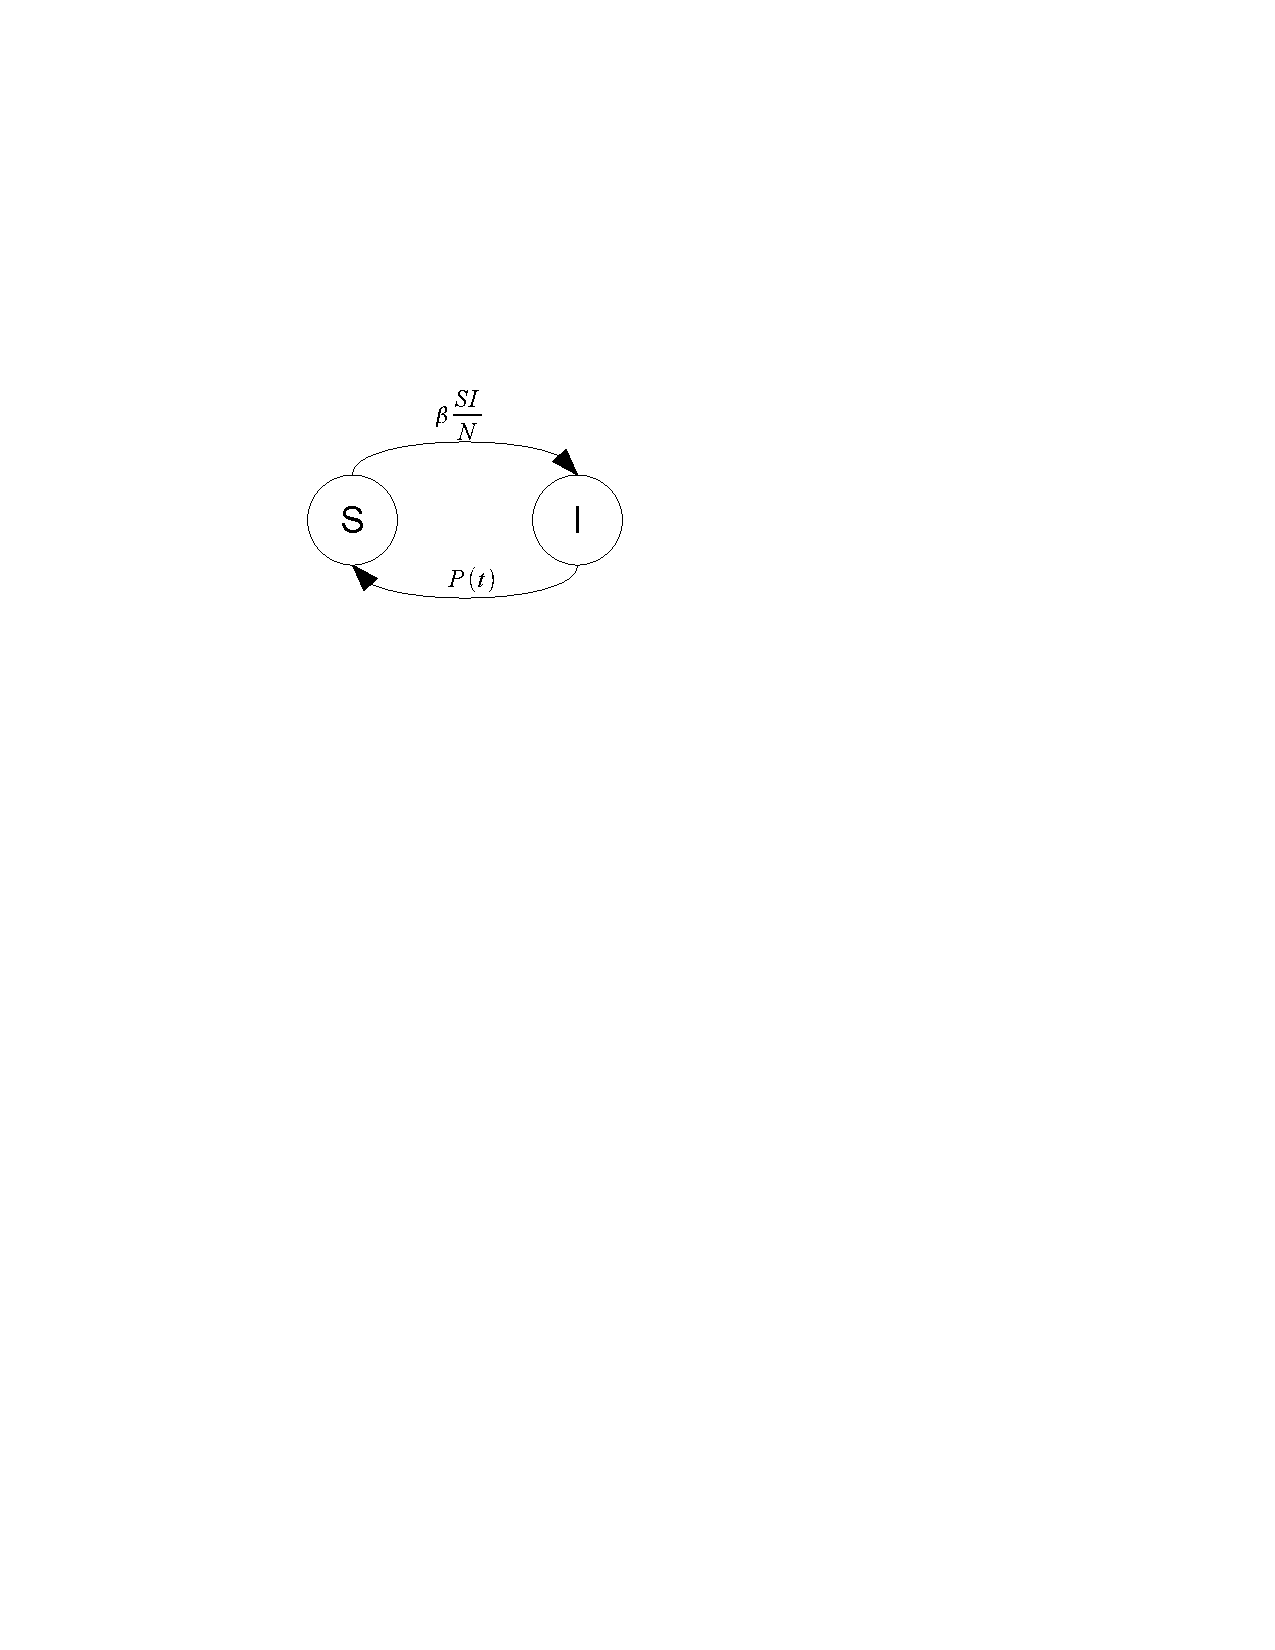
\includegraphics[width=0.45\textwidth]{../figs_03_residence_time/SIS_general}
\caption{The flow diagram of the model with arbitrary infectious period.}
\label{fig:flow_diagram_SIS_P}
\end{center}
\end{figure}
It details the flows of individuals between the compartments in the system.
It is extremely useful to rapidly understand what processes are modelled.


\frame{\frametitle{Reducing the dimension of the problem}
To formulate our model, we would in principle require an equation for $S$ and an equation for $I$.


But we have
\[
S(t)+I(t)=N, \textrm{ or equivalently, }S(t)=N-I(t).
\]
$N$ is constant (equal total population at time $t=0$), so we can deduce the value of $S(t)$, once we know $I(t)$, from the equation $S(t)=N-I(t)$.


We only need to consider 1 equation. {\bf Do this when possible!} (nonlinear systems are hard, one less equation can make a lot of difference)
}

\frame{\frametitle{Model for infectious individuals}
Integral equation for the number of infective individuals: 
\begin{equation}
I(t) = I_0(t)+ \int_0^t\beta\frac{(N-I(u))I(u)}{N} P(t-u) du
\label{eq:SIS_I} 
\end{equation}
\begin{itemize}
\item $I_0(t)$ number of individuals who were infective at time
$t=0$ and still are at time $t$.
\begin{itemize}
\item $I_0(t)$ is nonnegative, nonincreasing, and
such that $\lim_{t\to\infty}I_0(t)=0$.
\end{itemize}
\item $P(t-u)$ proportion of individuals who became infective at time $u$ and
who still are at time $t$.
\item $\beta (N-I(u))S(u)/N$ is $\beta S(u)I(u)/N$ with $S(u)=N-I(u)$, from the reduction of dimension.
\end{itemize}
}


\frame{\frametitle{Expression under the integral}
Integral equation for the number of infective individuals: 
\begin{equation}
I(t) = I_0(t)+ \int_0^t\beta\frac{(N-I(u))I(u)}{N} P(t-u) du
\tag{\ref{eq:SIS_I}} 
\end{equation}
The term
\[
\beta\frac{(N-I(u))I(u)}{N} P(t-u)
\]
\begin{itemize}
\item $\beta (N-I(u))I(u)/N$ is the rate at which new infectives are created, at time $u$,
\item multiplying by $P(t-u)$ gives the proportion of those who became infectives at time $u$ and who still are at time $t$.
\end{itemize}
Summing over $[0,t]$ gives the number of infective individuals at time $t$.
}


\frame{\frametitle{Case of an exponentially distributed time to recovery}
Suppose that $P(t)$ is such that the sojourn time in the infective
state has an exponential distribution with mean $1/\gamma$,
\emph{i.e.}, $P(t)=e^{-\gamma t}$.

Then the initial condition function $I_0(t)$ takes the form
\[
I_0(t)=I_0(0)e^{-\gamma t},
\]
with $I_0(0)$ the number of infective individuals at time $t=0$. This is obtained by considering the cohort of initially infectious individuals, giving a model such as \eqref{eq:N_general}.
Equation (\ref{eq:SIS_I}) becomes
\begin{equation}\label{eq:I_ODE}
I(t)=I_0(0)e^{-\gamma t}+\int_0^t \beta\frac{(N-I(u))I(u)}{N} e^{-\gamma (t-u)}du.
\end{equation}
Taking the time derivative of \eqref{eq:I_ODE} yields
\begin{align*}
I'(t) &= -\gamma I_0(0)e^{-\gamma t}-\gamma\int_0^t \beta\frac{(N-I(u))I(u)}{N}e^{-\gamma(t-u)}du +\beta \frac{(N-I(t))I(t)}{N} \\
&= -\gamma\left(I_0(0)e^{-\gamma t}+
\int_0^t \beta\frac{(N-I(u))I(u)}{N}e^{-\gamma(t-u)}du\right)+\beta \frac{(N-I(t))I(t)}{N} \\
&= \beta \frac{(N-I(t))I(t)}{N}-\gamma I(t),
\end{align*}
which is the classical logistic type ordinary differential equation
(ODE) for $I$ in an SIS model without vital dynamics (no birth or death).
}

\frame{\frametitle{Case of a step function survival function}
Consider case where the time spent infected has survival function 
\[
P(t)=\begin{cases}
1, & 0\leq t\leq\omega,\\
0, & t>\omega.
\end{cases}
\]
i.e., the sojourn time in the infective state is a constant
$\omega>0$.
 
In this case (\ref{eq:SIS_I}) becomes
\begin{equation}\label{eq:I_DDE}
I(t)=I_0(t)+\int_{t-\omega}^t \beta\frac{(N-I(u))I(u)}{N} du.
\end{equation}
Here, it is more difficult to obtain an expression for $I_0(t)$. It is however assumed that $I_0(t)$ vanishes for $t>\omega$.
}

\frame{
When differentiated, \eqref{eq:I_DDE} gives, for $t\geq\omega$,
\[
I'(t)=I_0'(t)+\beta\frac{(N-I(t))I(t)}{N}
-\beta\frac{\left(N-I(t-\omega)\right)I(t-\omega)}{N}.
\]
Since $I_0(t)$ vanishes for $t>\omega$, this gives the delay
differential equation (DDE)
\[
I'(t)=\beta\frac{(N-I(t))I(t)}{N}
-\beta\frac{(N-I(t-\omega))I(t-\omega)}{N}.
\]
}

\section{Conclusion}
\begin{itemize}
\item The distribution of the time of sojourn in classes (compartments) plays an important role in determining the type of model that we deal with.
\item All compartmental ODE models, when they use terms of the form $\kappa X$, make the assumption that the time of sojourn in compartments is exponentially distributed.
\item At the other end of the spectrum, delay differential equations with discrete delay make the assumption of a constant sojourn time, equal for all individuals.
\item Both can be true sometimes.. but reality is often somewhere in between. See Figure~\ref{fig:exp_distrib_80years} for an example of how an exponential distribution, with its fat tail, overepresents long sojourn times.
\end{itemize}

\begin{figure}[htbp]
\begin{center}
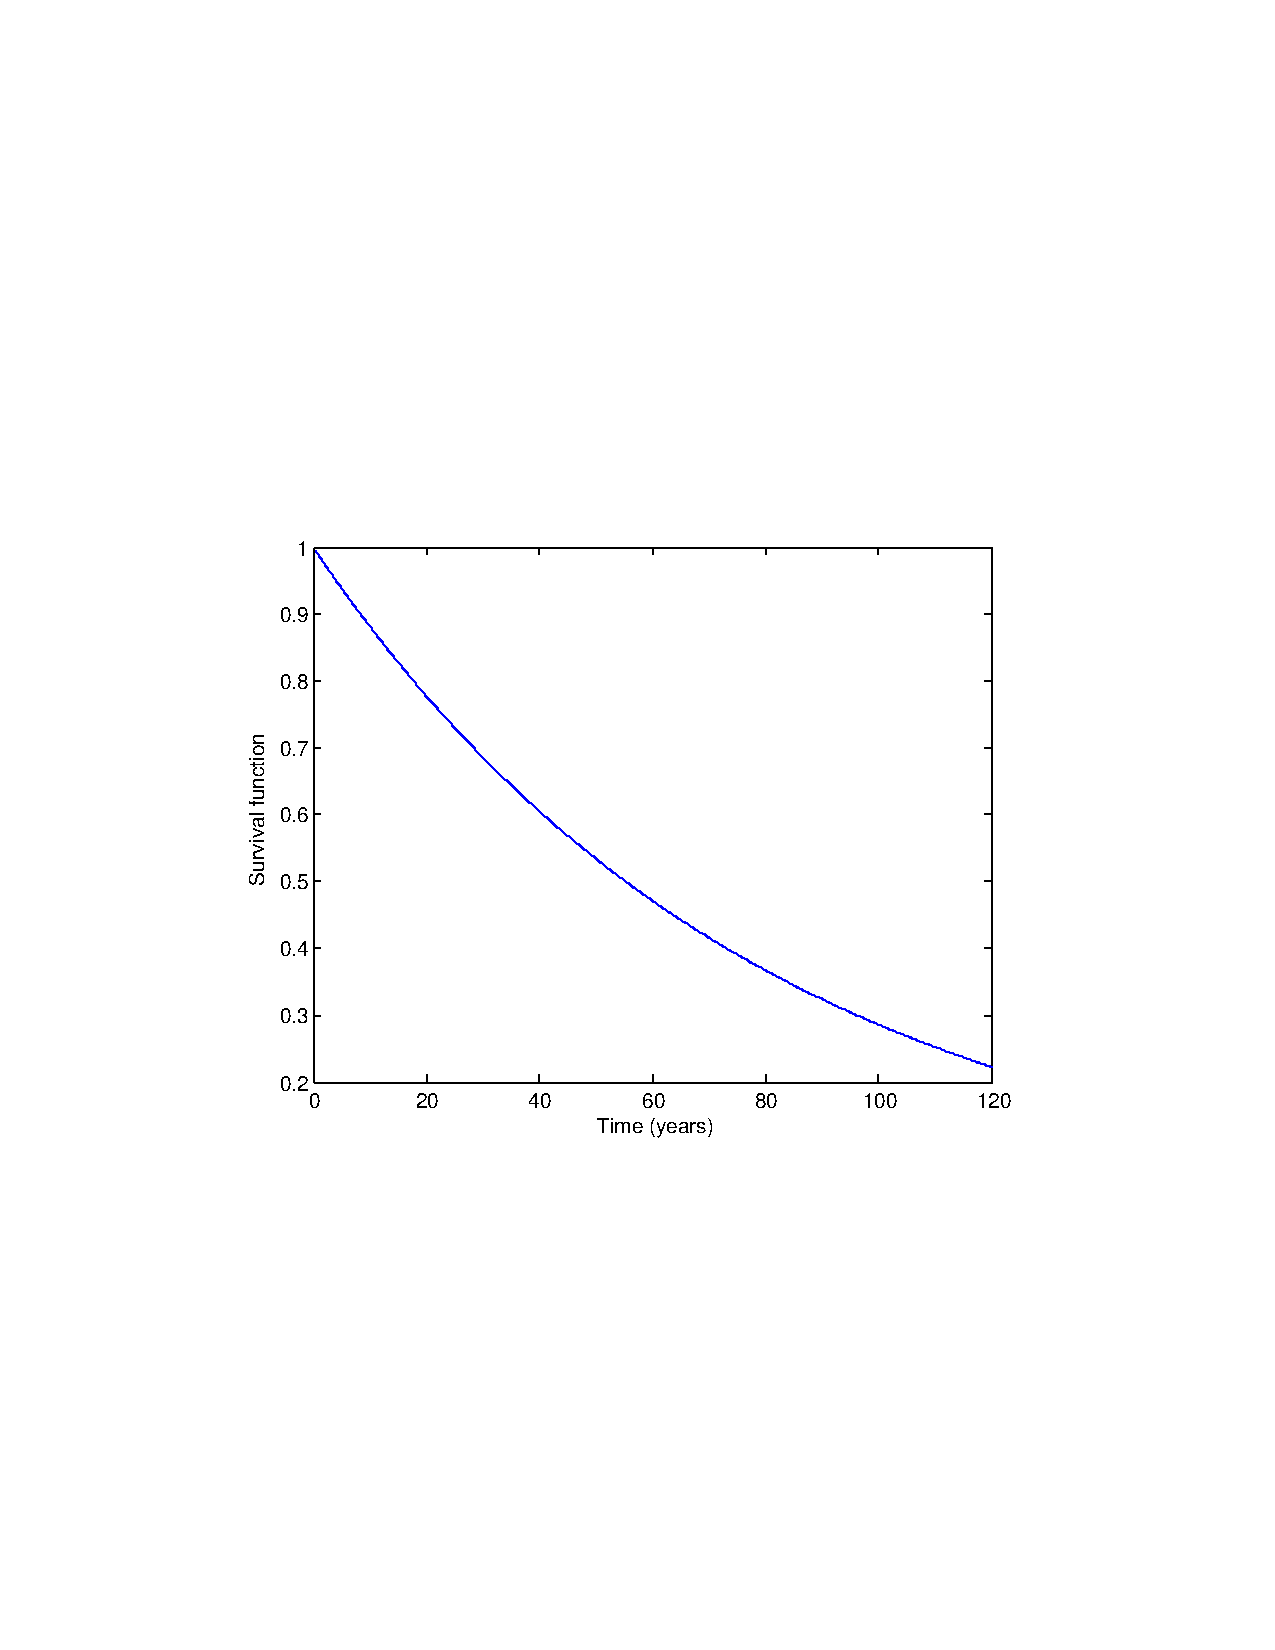
\includegraphics[width=0.5\textwidth]
{../figs_03_residence_time/survival_exp_80years}
\caption{Survival function, $\S(t)=\Proba{T>t}$, for an exponential distribution with mean 80 years. Note that this implies that more than 20\% of individuals in a cohort survive past the age of 120 years.}
\label{fig:exp_distrib_80years}
\end{center}
\end{figure}

%\frame{
%The \textbf{basic reproduction number}, denoted by $\Rzero$, which is a
%key concept in mathematical epidemiology, is now introduced. 
%It is defined as
%the expected number of secondary cases produced, in a completely
%susceptible population, by the introduction of a typical infective
%individual.  
%For this ODE model, $\Rzero=\beta/\gamma$.
%In terms of stability, the disease free equilibrium (DFE) with $I=0$
%is stable for $\Rzero<1$ and unstable for $\Rzero>1$. 
%At the threshold $\Rzero=1$, there is a forward bifurcation
%with a stable endemic equilibrium (with $I>0$) for $\Rzero>1$. Thus
%the value of $\Rzero$ determines whether the disease dies out or tends
%to an endemic value.
%}


\part{Deterministic discrete time systems} 
\chapter{A brief theory of discrete time systems}
\label{chap:theory_discrete_time}

In this chapter, we consider discrete-time systems of the form
\begin{equation}\label{sys:discret}
x_{t+1}=f(x_t),
\end{equation}
with initial condition given for $t=0$ by $x_0$, with $x,x_0\in\IR^n$ and $f:\IR^n\to\IR^n$.
We also consider $p$th order equations of the form
\begin{equation}\label{eq:nth_order_discrete}
f(x_{t+p},x_{t+p-1},\dots,x_{t+1},x_t,t)=0,
\end{equation}
where $f$ is a real-valued function of the real variables $x_t$ through $x_{t+p}$ and $t$. We could also consider systems of $n$th order equations, but for the sake of brievety, we will limit ourselves to equations of the form \eqref{sys:discret} and \eqref{eq:nth_order_discrete}.

Implicit in \eqref{sys:discret} and \eqref{eq:nth_order_discrete} is that the time interval is taken to be $\Delta t=1$. Also, the state of the system at time $t$ is denoted $x_t$. Formally, \eqref{sys:discret} should be written
\[
x(t+\Delta t)=f(x(t)),
\]
but this is cumbersome and will be used only when ambiguity could lead to miscomprehensions.

Using \eqref{sys:discret}, we see that
\begin{align*}
x_1 &= f(x_0) \\
x_2 &= f(x_1)= f(f(x_0))\stackrel{\Delta}{=} f^2(x_0) \\
& \vdots \\
x_k &= f^k(x_0).
\end{align*}
The compositions
\[
f^k=\underbrace{f\circ f\circ\cdots\circ f}_{k\textrm{ times}}
\]
are called the \textbf{iterates} of $f$.
They define an infinite sequence of points
\[
x_0,x_1,x_2,\ldots,x_t,\ldots,
\]
that constitute the \textbf{solution} to \eqref{sys:discret}. The object of this chapter is to determine the behavior of this solution. For example, in the case of the logistic map \eqref{eq:logistic_map}, do solutions behave like they do for the continuous time logistic equation \eqref{eq:ODE_logistic} and tend to the carrying capacity $K$?


\section{Types of equations/systems}
% \begin{definition}
% A difference equation of order $k$ has the form $$f(x_{t+k},x_{t+k-1},\dots,x_{t+1},x_t,t)=0\quad t=0,1,\dots,$$
% where $f$ is a real-valued function of the real variable $x_t$ through $x_{t+k}$ and $t$.
% \end{definition}
\begin{definition}
The \emph{order} of a difference equation \eqref{eq:nth_order_discrete} is the difference between the largest and the smallest arguments $p$ appearing in it.
\end{definition}
Remark that in biological terms, the order $p$ of the equation is the number of previous generations that directly influence the value of $x$ in a given generation.



\begin{definition}
The difference equation is called \emph{autonomous} if $f$ does not depend explicitly on $t$ and it is called \emph{nonautonomous} otherwise.
\end{definition}



\begin{definition}
Let 
\[
x_{t+p}+a_1 x_{t+p-1}+a_2 x_{t+p-2}+\dots +a_{p-1} x_{t+1}=b_t.
\]
If the coefficients $a_j$, $j=1,\dots,p$ are constant or depend on $t$ but \textbf{do not} depend on the state variables, then the difference equation is said to be \emph{linear}; otherwise, it is \emph{nonlinear}. 
\end{definition}

\begin{definition}
If the difference equation is linear and $b_t=0$ for all $t$, then it is said to be \emph{homogeneous}; otherwise, it is said to be \emph{nonhomogeneous}.
\end{definition}



\begin{definition}
A solution of the difference equation
$$f(x_{t+k},x_{t+k-1},\dots,x_{t+1},x_t,t)=0$$
is a function $x_t$, $t=0,1,2,\dots$ such that when substituted into the equation makes it a true statement.
\end{definition}





Some characteristics of difference equations
\begin{itemize}
\item changes of states are descibed over discrete intervals. Length of the discrete interval is some fixed length $\Delta t$: states of a system are modeled at the discrete time $t=0,\Delta t, 2\Delta t, \dots$
\item recurrence relation
\item evolutionary character or not
\item to describe populations whose generations do not overlap:
\end{itemize}




\section{First-order linear difference equation}
\begin{proposition}
Consider the first-order linear homogeneous difference equation with constant coefficients
\begin{equation}\label{eq:1st_order_linearDE}
x_{t+1}=ax_t
\end{equation}
If an initial value $x_0$ is known, the solution is unique and is given by 
\begin{equation}\label{eq:sol_1storder_linear_DE}
x_t=a^tx_0.
\end{equation}
\end{proposition}

\begin{proof}
We have
\[
x_1=ax_0,
\]
and so
$$x_2=ax_1=aax_0=a^2 x_0,$$
and
$$x_3=ax_2=aaax_0=a^3x_0 \dots$$
Continuing, we have the general expression
\[
x_t=a^tx_0.\qedhere
\]
\end{proof}

Clearly, \eqref{eq:sol_1storder_linear_DE} defines a geometric sequence with common ratio $a$. Therefore, the \textbf{asymptotic behavior} of the solution depends on the value of $a$:
\begin{itemize}
\item if $|a|<1$, then $\lim_{t\rightarrow \infty}x_t=0$, i.e., $x_t$ converges to 0,
\item if $a=1$, then for all $t\geq 0$, $x_t=x_0$, i.e., $x_t$ remains constant,
\item if $a=-1$, then for all $t\geq 0$, $x_t=(-1)^tx_0$, i.e., $x_t$ alternates,
\item if $|a|>1$ then $x_t$ diverges (either approaches infinity if $a>1$ or diverges with alternating signs if $a<-1$).
\end{itemize}


\begin{proposition}
Consider the first-order linear homogeneous difference equation defined for $t=0,1,2,\dots$ by
\[
x_{t+1}=a_tx_t.
\]
If an initial value $x_0$ is known, then the solution is unique and is given by
\[
x_t=\left [\prod_{i=0}^{t-1} a_i\right ]x_0.
\]
\end{proposition}

\begin{proof}
Let us prove by mathematical induction that the proposition $P_t$ holds $\forall t\in \IN\setminus\{0\}$, with
\[
P_t: \quad x_t=\left [\prod_{i=0}^{t-1} a_i\right ]x_0.
\]
First, we consider $P_1$. We have
$$x_1=a_0x_0,$$
hence $P_1$ is true. Then assume that $P_t$ is true, i.e., $x_t=\left [\prod_{i=0}^{t-1} a_i\right ]x_0$. Now express $x_{t+1}$:
\begin{align*}
x_{t+1} &= a_tx_t \\
&=a_t\left [\prod_{i=0}^{t-1} a_i\right ]\;x_0 \quad\textrm{(by induction hypothesis)}\\
&= \left [\prod_{i=0}^t a_i\right ]x_0,
\end{align*}
so $P_{t+1}$ is true.
By the principle of mathematical induction (PMI), we conclude that 
\[
x_t=\left [\prod_{i=0}^{t-1} a(i)\right ]x_0, \forall t\in \IN\setminus\{0\}.\qedhere
\]
\end{proof}


\begin{proposition}\label{Prop:FirstLinNonH}
Consider the first-order linear nonhomogeneous difference equation defined for $t=0,1,2,\dots$ by
$$x_{t+1}=a_tx_t + b_t.$$
If an initial value $x_0$ is known, then the solution is unique and is given by
\[
x_t=\left [\prod_{i=0}^{t-1} a_i\right ]x_0 +b_{t-1}+\sum_{i=0}^{t-2}\left [ \prod_{r=i+1}^{t-1} a_r \right]b_i.
\]
In particular,
\begin{itemize}
\item If $x_{t+1}=a x_t + b_t$, then 
$$x_t=a ^t x_0 +\sum_{i=0}^{t-1} a^{t-i-1}b(i).$$
\item If $x_{t+1}=a x_t + b$, then 
$$x_t=
\begin{cases}
a ^t x_0 +b\left[\dfrac{a^t-1}{a-1}\right] & a\not =1\\  
x_0 +bt & a =1.
\end{cases}
$$
\end{itemize}
\end{proposition}


\begin{proof}
Let us prove by mathematical induction that
\[
P_t:\quad
x_t=\left [\prod_{i=0}^{t-1} a_i\right ]x_0 +b_{t-1}+\sum_{i=0}^{t-2}\left [ \prod_{r=i+1}^{t-1} a_r \right]b_i
\]
holds true for all $t\in \IN\setminus\{0\}$.
At rank $t=2$: $x_1=a_0x_0+b_0$, then
$$x_2=a_1x_1+b_1=a_1a_0x_0+a_1b_0+b_1.$$
%Similarly for $x_3$
%$$x_3=a(2)x_2+b(2)=a(2)a(1)a(0)x_0+a(2)a(1)b(0)+a(2)b(1)+b(2)$$
Now assume that $P_t$ holds true, i.e., 
$$x_t=\left [\prod_{i=0}^{t-1} a_i\right ]x_0 +b_{t-1}+\sum_{i=0}^{t-2}\left [ \prod_{r=i+1}^{t-1} a_r \right]b_i$$
and express $x_{t+1}$:
\begin{align*}
x_{t+1} &= a_tx_t+b_t \\
&=a_t\left\{\left[\prod_{i=0}^{t-1} a_i\right]x_0 +b_{t-1}
+\sum_{i=0}^{t-2}\left[\prod_{r=i+1}^{t-1} a_r \right]b_i \right\}+b_t \\
&=\left[a_t\prod_{i=0}^{t-1} a_i\right ]x_0+a_tb_{t-1}+\sum_{i=0}^{t-2}\left [ a_t\prod_{r=i+1}^{t-1} a_r \right]b_i+b_t \\
&=\left [\prod_{i=0}^{t} a_i\right ]x_0+b_t+a_tb_{t-1}+\sum_{i=0}^{t-2}\left [ \prod_{r=i+1}^{t} a_r \right]b_i \\
&= \left [\prod_{i=0}^{t} a_i\right ]x_0+b_t
+\sum_{i=0}^{t-1}\left [ \prod_{r=i+1}^{t} a_r \right]b_i.
\end{align*}
Thus $P_{t+1}$ holds.
By the principle of mathematical induction, we conclude that, for all $t\in\IN\setminus\{0\}$, 
$$x_t=\left [\prod_{i=0}^{t-1} a_i\right ]x_0 +b_{t-1}+\sum_{i=0}^{t-2}\left [ \prod_{r=i+1}^{t-1} a_r \right]b_i.\qedhere$$
\end{proof}

\section{Higher-order linear equations}
\begin{definition}
The functions $x_t^1$, $x_t^2$,$\dots, x_t^k$ are said to be linearly independent for $t\geq t_0$ whenever 
$$a_1x^1_t+a_2x^2_t+\dots + a_kx^k_t=0$$
for all $t\geq t_0$, then we must have $a_1=a_2= \dots =a_k=0$.
\end{definition}

\begin{definition}
The Casoratian of $k$ functions $x_t^1$, $x_t^2$,$\dots, x_t^k$ is
$$C(x_t^1, x_t^2,\dots, x_t^k)=\det \left (
\begin{array}{cccc}
x_t^1 & x_t^2 & \dots & x_t^k\\
x_{t+1}^1 & x_{t+1}^2 & \dots & x_{t+1}^k\\
x_{t+2}^1 & x_{t+2}^2 & \dots & x_{t+2}^k\\
\vdots & & &\\
x_{t+k-1}^1 & x_{t+k-1}^2 & \dots & x_{t+k-1}^k\\
\end{array}\right )$$
\end{definition}

\begin{proposition}
If the Casoratian of $x_t^1$, $x_t^2$,$\dots, x_t^k$ satifies
$$C(x_t^1, x_t^2,\dots, x_t^k)\not =0 \quad \forall t$$
then $x_t^1$, $x_t^2$,$\dots, x_t^k$  are $k$ linearly independent functions.
\end{proposition}

\begin{definition}
A set of $k$ linearly independent solutions of a $k^{th}$ linear homogeneous difference equation is called a fundamental set of solutions.
\end{definition}

\begin{proposition}(Principle of superposition)
If $x_t^1$, $x_t^2$,$\dots, x_t^k$ are solutions a $k^{th}$ linear homogeneous difference equation then $$c_1x_t^1+c_2x_t^2+\dots, c_kx_t^k$$
is also solution of the $k^{th}$ linear homogeneous difference equation.
\end{proposition}

\begin{definition}
Let $\{x_t^1, x_t^2,\dots, x_t^k\}$ be a fundamental set of solutions of $k^{th}$ linear homogeneous difference equation. Then the general solution of the  $k^{th}$ linear homogeneous difference equation is given by $$x_t=\sum_{i=1}^kc_ix^i_t,$$ for arbitrary constants $c_i$, $i=1,\dots, k$
\end{definition}

\subsection[Homogeneous autonomous higher-order linear equations]{Homogeneous equations with constant coefficients}
The case of a second-order equation is derived to illustrate this subsection.

A second-order linear homogeneous equation with constant coefficients:
\begin{equation}\label{eq:SecLinHom}
a_0x_{t+2}+a_1x_{t+1}+ a_2 x_{t}=0
\end{equation}
To find two linearly independent solutions, $x_t^1$ and $x_t^2$: assume that solutions take the form of 
$x_t=\lambda ^t$ with $\lambda \not= 0$. Then substitute solution in \eqref{eq:SecLinHom}
$$a_0\lambda ^{t+2}+a_1\lambda ^{t+1}+ a_2 \lambda ^{t}=0,$$
$$a_0\lambda ^{2}+a_1\lambda + a_2 =0.$$

The equation $a_0\lambda ^{2}+a_1\lambda + a_2 =0$ is the \textbf{characteristic equation} of \eqref{eq:SecLinHom}. The 2 roots of the characteristic equation, $\lambda_1$ and $\lambda_2$, are the \textbf{eigenvalues}.

The general solution is a linear combination of the 2 solutions $x_t^1=\lambda_1^t$ and $x_t^2=\lambda_2^t$. The form of the general solution depends on the eigenvalues and there are 3 cases:
\begin{description}
\item[Eigenvalues are real and distinct:] $\lambda _1 \not = \lambda _2 $. The general solution is
$$x_t=c_1\lambda _1 ^t+c_2\lambda _2 ^t,$$
with $c_1$ and $c_2$ arbitrary constants.
\item[Eigenvalues are real and equal:] $\lambda _1  = \lambda _2 $. Then the $2$ linearly independent solutions are  $x_t^1=\lambda _1^t$ $x_t^2=t\lambda _2^t$. 
The general solution is
$$x_t=c_1\lambda _1 ^t+c_2t\lambda _2 ^t,$$
with $c_1$ and $c_2$ arbitrary constants.
\item[Eigenvalues are complex conjugates:] $\lambda _{1,2}=A\pm iB=r(\cos \phi \pm i \sin \phi)$, where $r=\sqrt{A^2+B^2}$ and $\phi=\arctan(B/A)$. The two linearly independent solutions are $x^1=r^t\cos(t\phi)$ and $x^2=r^t\sin (t\phi)$.
Then the general solution is
$$x_t=c_1 r^t\cos(t\phi)+c_2r^t\sin (t\phi),$$
with $c_1$ and $c_2$ arbitrary constants.
\begin{center}
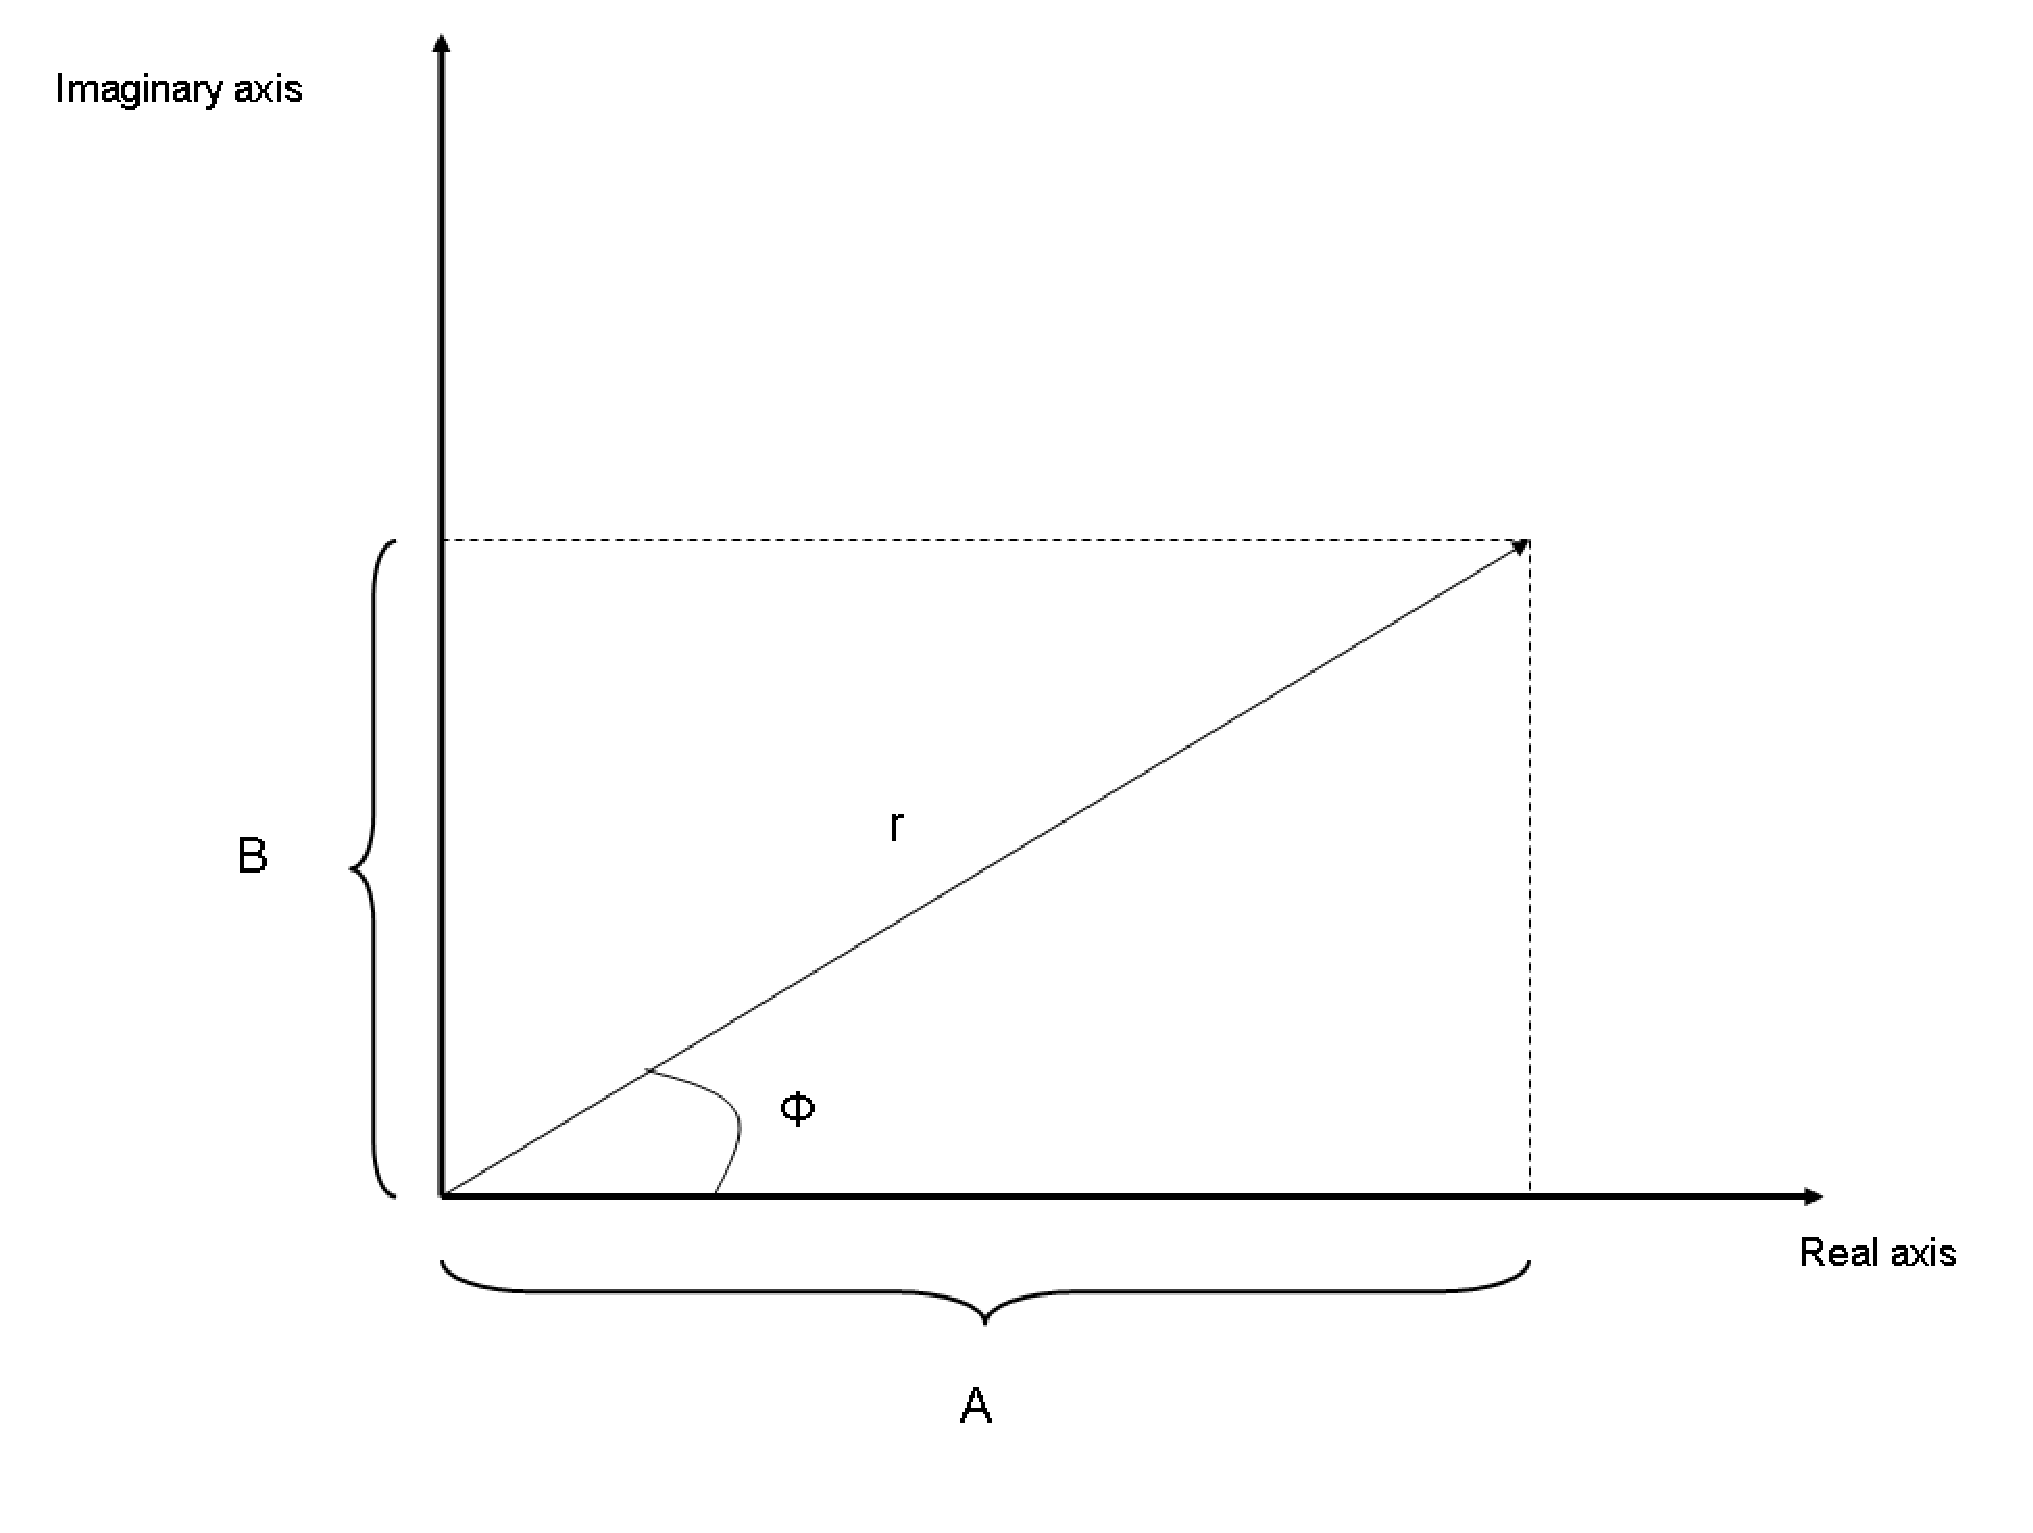
\includegraphics[width=.5\textwidth]{figs_steph/FigurePhase}
\end{center}
\end{description}


An $m^{th}-$order linear homogeneous equation with constant coefficients is defined as
\begin{equation}\label{eq:LinH}
a_0x_{t+m}+a_1x_{t+m-1}+\dots + a_m x_{t}=0
\end{equation}
Solutions are composed of linear superpositions of $m$ solutions of the form 
$x_t=\lambda ^t$, $\lambda \not = 0$
where $\lambda$ are obtained by finding the roots (eigenvalues) of the characteristic equation
$$a_0\lambda^{m}+a_1\lambda^{m-1}+\dots + a_m =0.$$
The characteristic equation has $m$ eigenvalues: $\lambda _i,$ $i=1,\dots, m$. 

If eigenvalues are all real and distinct, the general solution takes the form
$$x_t=c_1\lambda_1^t+\dots +c_m\lambda_m^t$$
where $c_i$, $i=1,\dots ,m$ are arbitrary.

For the other cases, general solutions depend on the existence of repeated or complex conjugate eigenvalues. If there is a real eigenvalue $\lambda _1$ of multiplicity $k$, then $k$ linearly independent solutions can be formed by multiplying by powers of $t$:
$$\lambda_1 ^t, t \lambda_1 ^t, t^2\lambda_1 ^t, \dots , t^{k-1}\lambda_1 ^t.$$
If there are complex eigenvalues $\lambda _{1,2}=r(\cos \phi \pm i \sin \phi)$ of multiplicty $k$, then there are $2k$ linearly independent solutions:
$$r^t\cos(t\phi),r^t\sin (t\phi),tr^t\cos(t\phi),tr^t\sin (t\phi),\dots,t^{k-1}r^t\cos(t\phi),t^{k-1}r^t\sin (t\phi)$$




\subsection{Nonhomogeneous equations}
An $m^{th}-$order linear nonhomogeneous equation  is defined as
\begin{equation}\label{eq:LinNonH}
a_0x_{t+m}+a_1x_{t+m-1}+\dots + a_m x_{t}=b(t)
\end{equation}

\begin{theorem}
The general solution of \eqref{eq:LinNonH} is
$$x_t=x_t^p+\sum_{i=1}^m a_i x_t^i$$
where $x_t^p$ is a particular solution of the nonhomogeneous equation and $\{x_t^1, x_t^2,\dots, x_t^k\}$ is a fundamental set of solutions of $m^{th}$ homogeneous equation \eqref{eq:LinH}.
\end{theorem}


To find a particular solution of a nonhomogeneous equation, there exist several methods:
\begin{description}
\item[Method of undetermined coefficient:] making a guess as to the form of the particular solution, and then substituting this function in the difference equation. This method works if the nonhomogeneous term $b(t)$ is a linear combination or product of terms having one of the forms
$$a^t, \quad \cos(ct), \quad  \sin(ct), \quad t^k.$$
See Table \ref{Table1}.
\item[Method of variation of constants]
\end{description}

\begin{table}
\begin{center}
\begin{tabular}{c|p{7cm}}
$b(t)$ & \multicolumn{1}{c}{$x_t^p$}
\\\hline
$a^t$ & $c_1 a^t$\\
$t^k$ & $c_0+c_1t+c_2t^2+\dots+c_k t^k$\\
$t^ka^t$ & $c_0a^t+c_1ta^t+c_2t^2a^t+\dots+c_k t^ka^t$\\
$\sin(ct),\cos(ct)$ & $c_1\sin(ct)+c_2\cos(ct)$\\
$a^t\sin(ct),a^t\cos(ct)$ & $(c_1\sin(ct)+c_2\cos(ct))a^t$\\
$a^tt^k\sin(ct),a^tt^k\cos(ct)$ & $(d_0+d_1t+d_2t^2+\dots+d_k t^k)\sin(ct)a^t+(c_0+c_1t+c_2t^2+\dots+c_k t^k)\cos(ct)a^t$\\
\end{tabular}
\label{Table1}
\caption{Particular solutions}
\end{center}
\end{table}


\subsection{Qualitative analysis}
What is the long-term behaviour of the solutions?

For linear difference equations, the asymptotic behavior depends on the eigenvalues: real and complex and the magnitude of eigenvalues.

\begin{definition}
Magnitude of an eigenvalue:
\begin{itemize}
\item If $\lambda=A$ is real, $|\lambda|=|A|$.
\item If $\lambda=A+iB$ is complex, $|\lambda|=|A+iB|=\sqrt{A^2+B^2}$.
\end{itemize}
\end{definition}


\begin{definition}
An eigenvalue $\lambda _i$ such that
$$|\lambda _i|\geq |\lambda _j|$$
for all $j\not =i$ is called the dominant eigenvalue. If the inequality is strict, then $\lambda _i$ is a strictly dominant eigenvalue.
\end{definition}

%\begin{itemize}
%\end{itemize}

Let the general solution of \eqref{eq:LinH} be
$$x_t=\sum_{i=1}^m c_i \lambda_i^t$$

The limiting behavior of the general solution is determined by the behavior of the dominant solution (correspondant to the dominant eigenvalue). Let $\lambda _1$ be the strictly dominant eigenvalue ($|\lambda _1|> |\lambda _j|$ for all $j\not =1$) then
$$x_t=\lambda _1^t\left[ c_1+\sum_{i=2}^m c_i\left ( \frac{\lambda_i}{\lambda_1}\right )^t\right ]$$
Since $\left |\frac{\lambda _i}{\lambda _1}\right |<1$, for all $i\not =1$, then $\left ( \frac{\lambda_i}{\lambda_1}\right )^t\rightarrow 0$ as $t\rightarrow +\infty$. Then $$\lim _{t\rightarrow +\infty }x_t=\lim _{t\rightarrow +\infty }c_1\lambda _1^t.$$
Depending on the value of $\lambda _1$ there are different situations
\begin{itemize}
\item $\lambda _1$ Real
\begin{itemize}
\item $\lambda _1 >1:$ $\lim _{t\rightarrow +\infty }c_1\lambda _1^t=\infty$ (monotonically diverge $\Rightarrow$ unstable system)
\item $\lambda _1 =1:$ constant
\item $0 <\lambda _1 <1:$ $\lim _{t\rightarrow +\infty }c_1\lambda _1^t=0$ (monotonically decreasing to 0 $\Rightarrow$ stable system)
\item $-1 <\lambda _1 <0:$ $\lim _{t\rightarrow +\infty }c_1\lambda _1^t=0$ (oscillating around zero and converging to 0 $\Rightarrow$ stable system)
\item $\lambda _1 =-1:$ system oscillating between two values $c_1$ and $-c_1$
\item $\lambda _1 <-1:$ system is oscillating but increasing in magnitude (unstable system)
\end{itemize}
\item $\lambda _1$ Complex
\begin{itemize}
\item $|\lambda _1|>1$: system oscillates but increases in magnitude (unstable system)
\item $|\lambda _1|=1$: system oscillates but constant magnitude 
\item $|\lambda _1|<1$: system oscillates but converges to 0 (stable system)
\end{itemize}
\end{itemize}

Magnitude of eigenvalues determine whether solutions are unbounded or bounded. The nature, real or complex determine whether solutions oscillate, or not.

In the case of a nonhomogeneous difference equation with a constant nonhomogeneous term, if the system converges, it will converge to the equilibrium point $x^*$ (not to $0$ as previously).



\section{First-order linear systems}
A higher-order linear difference equation can be converted to a first-order linear system.
Consider the $m^{th}$-order linear nonhomogeneous equation 
\[
a_0x_{t+m}+a_1x_{t+m-1}+\dots + a_m x_{t}=b(t).
\]
For convenience $x_t$ is now denoted $x(t)$. Let $Y(t)$ be a $m$-vector  $Y(t)=(y_1(t),y_2(t),\dots, y_m(t))$ that satisfies
\begin{align*}
y_1(t)&=x(t)\\
y_2(t)&=x(t+1)\\
y_3(t)&=x(t+2)\\
\vdots& \\
y_{m}(t)&=x(t+m-1).
\end{align*}
The first element $y_1(t)$ is the solution $x(t)$. Hence a first-order difference equation in $y$ is 
\begin{align*}
y_1(t+1)&=y_2(t)\\
y_2(t+1)&=y_3(t)\\
y_3(t+1)&=y_4(t)\\
\vdots &\\
y_{m-1}(t+1)&=y_{m}(t)\\
y_{m}(t+1)&=-a_1 y_m(t)-\dots -a_{m-1}y_2(t)- a_m y_1(t)+b(t)
\end{align*}
In matrix form,
$$Y(t+1)=AY(t)+B$$
where
$$A=\left (
\begin{array}{ccccc}
0 & 1 & 0 & \hdots & 0\\
0 & 0 & 1 & \hdots & 0\\
\vdots & \vdots & \vdots & \ddots & \vdots\\
0 & 0 & 0 & \hdots & 1\\
-a_{m} & -a_{m-1} & -a_{m-2} & \hdots & -a_{1}
\end{array}
\right), \quad B=\left ( \begin{array}{c}
0\\
0\\
\vdots\\
0\\
b(t)
\end{array}
\right).
$$ 
The matrix $A$ has 1's along the superdiagonal and has the coefficients of the higher-order difference equation $-a_i$ (but the signs are reversed) along the last row. Matrix is called the {\bf companion matrix} of the $m^{th}-$order difference equation.


A solution to a first-order linear difference system $X(t+1)=AX(t)+B$ is the superposition of two solutions: the general solution $X_h$ to the homogeneous system $X_h(t+1)=AX_h(t)$ and a particular solution $X_p$ to the nonhomogeneous system $X_p(t+1)=AX_p(t)+B$. The general solution to the nonhomogeneous system is $$X(t)=X_h(t)+X_p(t).$$


The homogeneous system has $m-$linearly independent solutions: there are some direct and indirect methods to find these linearly independent solutions.

{\bf Indirect methods} use the fact that the solution can be expressed as $X(t)=A^tX(0). $ In \cite{Elaydi1998}, methods to compute $A^t$ are presented, then the general solution can be known.

{\bf Direct method} to solve $X(t+1)=AX(t)$ where $A=(a_{ij})$ is an $m\times m$ constant matrix:
Assume that a solution has the following form $X(t)=\lambda ^t V$ where $V$ is an nonzero $m-$column vector and $\lambda$ is a constant. Substituting $\lambda ^t V$ into the linear system gives
$$\lambda ^{t+1} V=A\lambda ^t V,$$
then
\begin{equation}(A - \lambda I) V=\mathbf{0}\label{eq:Cha}\end{equation}
where $I$ is the $m\times m$ identity matrix and $\mathbf{0}$ is the zero vector. The zero solution $V=0$ is the trivial solution; and \eqref{eq:Cha} has an unique solution if $\det(A - \lambda I)\not =0$. Hence, nonzero solutions $V$ are obtained if and only if $(A - \lambda I) $ is singular if and only if 
\begin{equation}\det(A - \lambda I) =0.\label{eq:Charac}\end{equation}

Equation \eqref{eq:Charac} is referred as the {\bf characteristic equation of matrix} $A$. The $m$ solutions $\lambda_i$, $i=1,\dots, m$ of \eqref{eq:Charac} are called the {\bf eigenvalues} of the matrix $A$. The nonzero solutions $V_i$ are the {\bf eigenvectors} corresponding to the eigenvalue $\lambda_i$ that are found by solving $(A - \lambda_i I) V_i=\mathbf{0}$.

Then the general solution is a linear combination of $m$ linearly independent solutions $X_i=\lambda _i ^t V_i$, $i=1,\dots, m$:
\begin{equation}X(t)=\sum_{i=1}^m c_i\lambda _i ^t V_i\label{eq:solFirstSyst}\end{equation}
where $c_i$ are arbitrary constants.

The asymptotic behavior of the solution \eqref{eq:solFirstSyst} does not require the knowlegde of the eigenvectors. The asymptotic behavior is determined by the eigenvalues and their magnitude.

\begin{definition}
The spectral radius of matrix $A$ is denoted $\rho(A)$ and is defined as
$$\rho(A)=\max_{i\in \{1,2,\dots,m\}}|\lambda_i|$$
\end{definition}


\begin{theorem}\label{Theo:NormRho}
Let $A$ be a $k\times k$ matrix
$$\rho(A)\leq \| A\| $$
\end{theorem}

Three usual matrix norms are
\begin{itemize}
\item $ \| A\|_1=\max_{1\leq j\leq k}\sum_{i=1}^k|a_{ij}|$ (sum over columns),
\item $ \|A\|_2=[\rho(A^TA)]^{1/2}$
\item $\|A\|_{\infty}=\max_{1\leq i\leq k}\sum_{j=1}^k|a_{ij}|$ (sum over rows).
\end{itemize}








\begin{theorem}\label{Theorem:MatrixConverg}
Let $A$ be a constant $m \times m$ matrix. Then the spectral radius of $A$ satisfies $\rho(A)<1$ if and only if $$\lim_{t\rightarrow + \infty}A^t=\mathbf{0}$$
\end{theorem}

As the solution of $X(t+1)=AX(t)$ is $X(t)=A^tX(0)$, $\lim_{t\rightarrow + \infty} X(t)=0$ when $\rho(A)<1$.

\subsection{Nonnegative matrices}
\begin{definition}
A matrix $A$ whose entries are nonnegative is called a nonnegative matrix, denoted $A\geq 0$.
\end{definition}


\begin{definition}
A matrix $A$ whose entries are positive is called a positive matrix, denoted $A> 0$.
\end{definition}


\begin{definition}
A square $m\times m$  matrix $A=a_{ij}$ is \textbf{reducible} if the index set $1,2, \dots, m$ can be split into two nonempty complementary sets $S_1$ and $S_2$: $S_1=\{i_1,\dots , i_{\mu}\}$ and $S_2=\{k_1,\dots , k_{\varepsilon}\}$ where $m=\mu+\varepsilon$ such that
$$a_{i_\alpha k_{\beta}}=0 \quad (\alpha = 1,2,\dots , \mu; \beta = 1,2, \dots, \varepsilon).$$
Otherwise, the matrix $A$ is \textbf{irreducible}.
\end{definition}


\begin{definition}
If there exits a directed path from node $i$ to $j$ for every node $i$ and $j$ in the digraph, then the digraph is said to be strongly connected.
\end{definition}

\begin{theorem}
The digraph of matrix $A$ is strongly connected if and only if $A$ is irreductible.
\end{theorem}


\begin{theorem}(Frobenius Theorem)
An irreductible, nonnegative matrix $A$ always has a positive eigenvalues $\lambda$ that is a simple root (multiplicity one) of the characteristic equation. The value of $\lambda$ is greater than or equal to the magnitude of all of the other eigenvalues. To the eignevalue $\lambda$ there corresponds an eigenvector with positive coordinates.
\end{theorem}


\begin{theorem}(Perron Theorem)
A positive matrix $A$ always has a real, positive eigenvalue $\lambda$ that is a simple root of the characteristic equation and exceeds the magnitude of all of the other eigenvalues
$$|\lambda _i|<|\lambda|,\quad \forall i.$$
To the eigenvalue $\lambda$ there corresponds an eigenvector with positive coordinates.
\end{theorem}


\begin{definition}
If an irreductible, nonnegative matrix $A$ has $h$ eigenvalues $\lambda _1, \lambda _2, \dots \lambda _h$ of maximum modulus ($|\lambda _1 |= |\lambda _i|, i=1,2,\dots ,h $), then $A$ is called primitive if $h=1$ and imprimitive if $h>1$. The value of $h$ is called the index of imprimitivity.
\end{definition}

The index of imprimitivity is the number of eigenvalues of matrix $A$ with maximum modulus (with magnitude equal to $\rho(A)$).

\begin{theorem}
A nonnegative matrix $A$ is primitive if and only if some power of $A$ is positive (i.e. $A^p>0$ for some integer $p\geq 1$).
\end{theorem}

\begin{theorem}\cite{BermanPlemmons1994}
A irreductible matrix is primitive if its trace if positive. 
\end{theorem}

The following theorem is one of the most important in the theory of matrices.
\begin{theorem}(Perron-Frobenius Theorem)
If $M$ is a nonnegative primitive matrix, then:
\begin{itemize}
\item $M$ has a positive eigenvalue $\lambda_1$ of maximum modulus.
\item $\lambda_1$ is a simple root of the characteristic polynomial.
\item for every other eigenvalue $\lambda _i$, $\lambda_1>\lambda_i$ (it is strictly dominant)
\item $$\min_{i}\sum_j m_{ij}\leq \lambda _1 \leq \max_{i}\sum_j m_{ij} $$
$$\min_{j}\sum_i m_{ij}\leq \lambda _1 \leq \max_{j}\sum_i m_{ij} $$
\item the row and column eigenvectors associated with $\lambda_1$ are strictly positive.
\item the sequence $M^t$ is asymptotically one-dimensional, its columns converge to the column eigenvector associated with $\lambda_1$; and its rows converges to the row eigenvector associated with $\lambda_1$.
\end{itemize}
\end{theorem}



\section{Fixed points}
For that, as in the continuous time case, we first seek equilibrium solutions, that is, solutions for which no variation occurs. Because of the type of equation that arises when seeking such solutions, equilibrium solutions are usually called fixed points, in the context of discrete-time systems.

\begin{definition}[Fixed point]
Let $f$ be a function. A point $p$ such that $f(p)=p$ is called a \textbf{fixed point} of $f$.
\end{definition}
The existence of fixed points is guaranteed in a relatively general situation by the following two theorems.
\begin{theorem}
Consider the closed interval $I=[a,b]$. If $f:I\to I$ is continuous, then $f$ has a fixed point in $I$.
\end{theorem}
\begin{theorem}
Let $I$ be a closed interval and $f:I\to\IR$ be a continuous function. If $f(I)\supset I$, then $f$ has a fixed point in $I$.
\end{theorem}

\begin{definition}[Periodic point]
Let $f$ be a function. If there exists a point $p$ and an integer $n$ such that
\[
f^n(p)=p,\quad\textrm{but}\quad f^k(p)\neq p\textrm{ for }k<n,
\]
then $p$ is a periodic point of $f$ with (least) period $n$ (or a $n$-periodic point of $f$).
\end{definition}
\vskip0.5cm
Thus, $p$ is a $n$-periodic point of $f$ iff $p$ is a $1$-periodic point of $f^n$.


\subsection{Local stability of fixed points and periodic points}
\begin{theorem}
Let $f$ be a continuously differentiable function (that is, differentiable with continuous derivative, or $C^1$), and $p$ be a fixed point of $f$. 
\begin{enumerate}
\item If $|f'(p)|<1$, then there is an open interval $\mathcal{I}\ni p$ such that $\lim_{k\to\infty}f^k(x)=p$ for all $x\in\mathcal{I}$.
\item If $|f'(p)|>1$, then there is an open interval $\mathcal{I}\ni p$ such that if $x\in\mathcal{I}$, $x\neq p$, then there exists $k$ such that $f^k(x)\not\in\mathcal{I}$.
\end{enumerate}
\end{theorem}
\begin{definition}
Suppose that $p$ is a $n$-periodic point of $f$, with $f\in C^1$. 
\begin{itemize}
\item If $|\left(f^n\right)'(p)|<1$, then $p$ is an \textbf{attracting} periodic point of $f$. 
\item If $|\left(f^n\right)'(p)|>1$, then $p$ is an \textbf{repelling} periodic point of $f$.
\end{itemize}
\end{definition}

\subsection{Bifurcations}
Consider an equation 
\begin{equation}
x_{t+1}=f_r(x_t),
\end{equation}
where $r$ is a parameter in $\IR$.
The function $f_r$ is called a \textbf{parametrized family} of functions.


\begin{definition}[Bifurcation]
Let $f_\mu$ be a parametrized family of functions. Then there is a \textbf{bifurcation} at $\mu=\mu_0$ (or $\mu_0$ is a bifurcation point) if there exists $\varepsilon>0$ such that, if $\mu_0-\varepsilon<a<\mu_0$ and $\mu_0<b<\mu_0+\varepsilon$, then the dynamics of $f_a(x)$ are ``different'' from the dynamics of $f_b(x)$.
\end{definition}
\vskip0.5cm
An example of ``different'' would be that $f_a$ has a fixed point (that is, a 1-periodic point) and $f_b$ has a 2-periodic point.

\subsection{Global stability}
\label{sec:global_stability}
The results presented here come from \cite{Allen2007}. We use the words \emph{equilbrium} and \emph{fixed point} interchangeably. Throughout this Section, we consider the discrete time scalar equation
\begin{equation}
x_{t+1}=f(x_t) \tag{\ref{sys:discret}}
\end{equation}
induced by the mapping $f$.

\begin{definition}[Globally attractive fixed point]
Suppose that $\bar x$ is a fixed point of $f$,
where $f: [0,a)\rightarrow [0,a),$ $0<a\leq \infty$. Then $\bar x$ is said to be \emph{globally attractive} if for all initial conditions $x_0\in (0,a)$, $$\lim_{t\rightarrow \infty}x_t=\bar x.$$
\end{definition}

\begin{definition}[Globally asymptotically stable fixed point]
The fixed point is said to be \emph{globally asymptotically stable} if $\bar x$ is globally attractive and if $\bar x$ is locally stable.
\end{definition}
Globally attractive equilibria are locally attractive, therefore globally asymptotically stable equilibria are locally asymptotically stable.






\section{Nonlinear difference equations}
Here, we study autonomous difference equations. The methods presented here also apply to the linear systems studied in the previous sections, although for linear systems, it is more efficient to use the specific tools that can be derived.

\subsection{Equilibrium solution - Periodic solution}
\begin{definition}\label{def:fixedpoint}
A point $x^*$ in the domain of $f$ is said to be an equilibrium point (an equilibrium solution) of the first-order difference equation $$x_{t+1}=f(x_t)$$ if it is a fixed point of $f$ \emph{i.e.} a constant solution that satisfies
$$f(x^*)=x^*.$$
\end{definition}
Graphically an equilibrium point is the $x-$coordinate of the point where the graph of $f(x)$ intersect the diagonal line $y=x$.


Same definition as in Definition \ref{def:fixedpoint} holds for a first-order system. For example, for a two-dimensional first order system
$$
\begin{array}{cc}
x_{t+1}=&f(x_t,y_t)\\
y_{t+1}=&g(x_t,y_t)
\end{array}
$$
the equilibrium solution is a solution $(\bar x, \bar y)$ such that $\bar x= f(\bar x,\bar y)$ and $\bar y=g(\bar x,\bar y)$.

\begin{quote}
Equilibrium solutions are biologically interesting because they represent the "resting states", the "stationary states" of the system. No change occurs from generation $t$ to generation $t+1$. 
\end{quote}



A difference equation takes the form
\[
x_{t+1}=f(x_t).
\]
Starting from an initial point $x_0$, we have
\begin{align*}
x_1 &= f(x_0) \\
x_2 &= f(x_1)=f(f(x_0))=f^2(x_0) \\
x_3 &= f(x_2)=f(f(f(x_0)))=f^3(x_0) \\
\ldots &\\
x_t &= f(f(f(\dots f(x_0))))=f^t(x_0)
\end{align*}
where the superscript $t$ is the number of time steps or iterations beginning from the initial value $x_0$. $f^m(x_0)$ is called the $m^{th}$ iterate of $f$.




\begin{definition}
A periodic solution of period $m>1$ of the difference equation $$x_{t+1}=f(x_t)$$ is a real-valued solution $\bar x_k$ satisfying
$$f^m(\bar x_k)=\bar x_k$$ and $$f^i(\bar x_k)\not =\bar x_k \quad i=1,2,\dots, m-1$$
\end{definition}

Note that an equilibrium point is a solution of period 1.
Graphically a periodic point is the $x-$coordinate of the point where the graph of $f^m(x)$ intersect the diagonal line $y=x$.



\begin{definition}
An $m-$cycle is a set of points $\{\bar x _1, \bar x_2, \dots , \bar x_m\}$ where for each $k=1,\dots,m$, $\bar x_k$ is a periodic solution of period $m$. The set $\{\bar x_1, f(\bar x_1), \dots , f^{m-1}(\bar x_1) \}$ is called a periodic orbit of $\bar x_1$
\end{definition}



\subsection{Local stability in first-order equations}
Local stability of an equilibrium solution implies that solutions approach the equilibrium only if they are initially close to it. Global stability of an equilibrium is much stronger: global stability implies that regardless of the initial condition, solutions approach the equilibrium.

An equilibrium is called locally asymptotically stable if for any small perturbation away from the equilibrium, the solution returns to the equilibrium value.

\begin{definition}[Local stability]
A equilibrium solution $\bar x$ of $x_{t+1}=f(x_t)$ is \emph{locally stable} if, for any  $\varepsilon>0$, there exists $\delta>0$ such that if $|x_0-\bar x|<\delta$, implies $$|x_t- \bar x|=|f^t(x_0)-\bar x|<\varepsilon \quad \forall t>0.$$ If a fixed point $\bar x$ is not stable, then it is \emph{unstable}.
\end{definition}


\begin{definition}[Local attractivity]
A equilibrium solution $\bar x$ is \emph{locally attracting} if there exists $\eta>0$ such that
\[
|x_0-\bar x|<\eta\quad\textrm{implies}\quad \lim_{t\to\infty}x_t=\bar x.
\]
If $\eta=\infty$, then $\bar x$ is a \emph{global attractor} (or is \emph{globally attracting}).
\end{definition}

\begin{definition}[Local asymptotic stability]
The equilibrium solution $\bar x$ is locally asymptotically stable if it is locally stable and locally attracting.
\end{definition}

%Local asymptotic stability is referred to as \emph{neighborhood stability}. Solutions that are locally asymptotically stable converge to the stable equilibrium if they begin in a small neighborhood of that equilibrium.

The convergence behavior for a first-order difference equation that is locally asymptotically stable may take the form of convergent oscillations or convergent exponential solutions. If the solution values tend to amplify and do note converge to the equilibrium,  the equilibrium is unstable. Such instability may appear as divergent oscillations or divergent exponential solutions. When the equilibrium is stable but not asymptotically stable it is said \emph{neutral stable}.


%To study local stability:
%\begin{itemize}
%\item identify the equilibrium solution
%\item linearization techniques to determine the behavior of solution near the equilibrium.
%\item If the equilibrium is stable for any set of initial condition, then the equilibrium is globally stable.
%\end{itemize}

\vspace{1cm}
Define the difference equation
\begin{equation}\label{eq:NonLin}
x_{t+1}=f(x_t)
\end{equation}
with an equilibrium solution $\bar x$. Let define a new variable
$$u_{t}=x_t-\bar x.$$
$u_t$ is a small quantity termed a perturbation of the equilibrium solution. Then $u_t$ satisfies the difference equation \eqref{eq:NonLin}
$$u_{t+1}=x_{t+1}-\bar x=f(x_t)-\bar x=f(u_t+\bar x)-f(\bar x)=g(u_t)$$
where $g(u)=f(u+\bar x)-f(\bar x)$.

Note that zero is a fixed point of $g$ if and only if $\bar x$ is a fixed point of $f$. In addition, zero is a locally stable (unstable, or locally asymptically stable) fixed point of $g$ if and only if $\bar x$ is a locally stable (unstable or locally asymptotically stable) fixed point of $f$. To find for the stability of $\bar x$ we assume that $f$ has a second order derivative in some interval $I$ containing $\bar x$, then by Taylor's approximation
$$f(x)=f(\bar x)+f'(\bar x)(x-\bar x)+\frac{f''(\epsilon)}{2!}(x-\bar x)^2$$
for $\epsilon \in I$. For $(x-\bar x)$ sufficiently small, we have the linear approximation
$$\underbrace{f(x_t)-\bar x}_{u_{t+1}}=f'(\bar x)\underbrace{(x_t-\bar x)}_{u_t},$$
then 
\begin{equation}\label{eq:Linearizatio}
u_{t+1}=f'(\bar x)u_t
\end{equation} is referred to as the \emph{linear approximation} to the difference equation \eqref{eq:NonLin} at the equilibrium $\bar x$.

If the initial condition are sufficiently close to $\bar x$, then the dynamics of $u_t$ is determined by the linearization \eqref{eq:Linearizatio}. In term of perturbation, to understand whether small perturbations $u_t$ from the equilibrium solution increase or decrease, we can solve \eqref{eq:Linearizatio} by using the difference equation method. We know that the solution of \eqref{eq:Linearizatio} will be decreasing whenever $|f'(\bar x)|<1$. Therefore, the value of $f'(\bar x)$ determines whether $\bar x$ is locally asymptotically stable or unstable.



\begin{theorem}[Condition for stability]
Assume  $f'$ is continuous on an open interval $I$ containing $\bar x$ and $\bar x$ is a fixed point of $f$. Then $\bar x$ is a locally asymptotically stable equilibrium of $x_{t+1}=f(x_t)$ if
$$|f'(\bar x)|<1$$
and unstable if $$|f'(\bar x)|>1$$
\end{theorem}




\begin{definition}
An equilibrium $\bar x$ of $$x_{t+1}=f(x_t)$$ is said to be hyperbolic if $|f'(\bar x)|\not =1$.

Otherwise ($|f'(\bar x)| =1$), it is said to be nonhyperbolic.
\end{definition}

\begin{theorem}
Suppose that $f'(\bar x) =1$ for an equilibrium solution $\bar x$ of $x_{t+1}=f(x_t)$, and $f'''$ is continuous on an open interval containing $\bar x$, then the following statement hold:
\begin{itemize}
\item $f''(\bar x)\not =0$, then the $\bar x$ is unstable.
\item $f''(\bar x)=0$ and $f'''(\bar x)>0$, then $\bar x$ is unstable.
\item $f''(\bar x)=0$ and $f'''(\bar x)<0$, then $\bar x$ is locally asymptotically stable.
\end{itemize}
\end{theorem}

\begin{definition}[Schwarzian derivative]
The Schwarzian derivative of a function $f$ at $x$ is denoted $(Sf)(x)$ and defined as follows:
$$(Sf)(x)=\frac{f'''(x)}{f'(x)}-\frac{3}{2}\left ( \frac{f''(x)}{f'(x)} \right )^2.$$
\end{definition}
Note that $f'(x)=-1$, $(Sf)(x)=-f'''(x)-\frac{3}{2} f''(x)^2.$
\begin{theorem}
Suppose that $f'(\bar x) =-1$ for an equilibrium solution $\bar x$ of $x_{t+1}=f(x_t)$, and $f'''$ is continuous on an open interval containing $\bar x$, then the following statement hold:
\begin{itemize}
\item $(Sf)(\bar x)>0$, then the $\bar x$ is unstable.
\item $(Sf)(\bar x)<0$, then $\bar x$ is locally asymptotically stable.
\end{itemize}
\end{theorem}




\begin{theorem}
Suppose $f'$ is continuous on an open interval $I$ and the $m-$cycle
$$\{\bar x_1, f(\bar x_1), \dots , f^{m-1}(\bar x_1)\}$$
of the difference equation $$x_{t+1}=f(x_t)$$ is contained in $I$. Then the $m-$cycle is locally asympotically stable if
$$\left| \frac{d[f^m(\bar x_k)]}{dx}\right|<1$$
for some $k$ and unstable if
$$\left| \frac{d[f^m(\bar x_k)]}{dx}\right|>1$$
for some $k$.
\end{theorem}



\begin{theorem}(Corollary)
Suppose $\{\bar x_1, \bar x_2, \dots , \bar x_m\}$ is an $m-$cycle of $x_{t+1}=f(x_t)$. Then the $m-$cycle is locally asymptotically stable if $$\left |   f'(\bar x_1)f'(\bar x_2)\dots f'(\bar x_m)\right |<1$$
\end{theorem}


Illustration: $\{\bar x_1,\bar x_2\}$ is a $2-$cycle that is locally asymptotically stable if and only if $$\left| \left . \frac{d[f]}{dx}\right |_{\bar x_1}\left . \frac{d[f]}{dx}\right |_{\bar x_2}\right|<1$$


\subsubsection{Cobwebbing method for first-order equation}
Graphical method to answer qualitative questions about the solution of $$x_{t+1}=f(x_t).$$

In the $(x_tx_{t+1})-$plane, sketch $x_{t+1}=x_{t}$ and $x_{t+1}=f(x_t)$:
\begin{itemize}
\item any intersections of these graphs is an equilibrium solution of the difference equation.
\item to investigate the behavior of the solutions
\begin{itemize}
\item choose a starting value $x_0$, and begin at the point $(x_0,x_0)$ in the $(x_tx_{t+1})-$plane.
\item draw a vertical line to the curve $x_{t+1}=f(x_t)$; this reaches the curve at $(x_0,f(x_0))=(x_0,x_1)$.
\item draw a horizontal line to the diagonal $x_{t+1}=x_t$; this reaches the diagonal at the point $(x_1,x_1)$.
\item Repeat the process to arrive at $(x_2,x_2)$ and indefinitely until the behavior of the equation with this starting value becomes clear.
\item If necessary, re-do the same with other starting values.
\end{itemize}
\end{itemize}




\subsection{Global stability in first-order equations}
Global stablity of an equilibrium removes the restrictions on the initial conditions. In global asympotic stability, solutions approach the equilibrium solution for all initial conditions. 


\begin{definition}
Suppose that $\bar x$ is an equilibrium solution of the difference equation $$x_{t+1}=f(x_t),$$
where $f: [0,a)\rightarrow [0,a),$ $0<a\leq \infty$. Then $\bar x$ is said to be globally attractive if for all initial conditions $x_0\in (0,a)$, $$\lim_{t\rightarrow \infty}x_t=\bar x.$$

The equilibrium is said to be globally asymptotically stable if $\bar x$ is globally attractive and if $\bar x$ is locally stable.
\end{definition}
Globally attractive equilibria are locally attractive, therefore globally asymptotically stable equilibria are locally asymptotically stable.




If $f$ is a continuous map, global attractivity is equivalent to global asymptotic stability.
\begin{theorem}\label{th:gas_1}
Suppose that for system \eqref{sys:discret}, the function $f$ satisfies
\begin{enumerate}
\item $f$ is continuous on $[0,a),$ $0<a\leq \infty$,
\item $f: [0,a)\rightarrow [0,a),$ $0<a\leq \infty$,
\item $0<f(x)<x$ for all $x\in [0,a)$.
\end{enumerate}
Then the origin is globally asymptotically stable for \eqref{sys:discret}.
\end{theorem}



The following provide necessary and sufficient conditions for global asymptotic stability of a positive equilibrium $\bar x$.
\begin{theorem}\label{th:gas_2}
The difference equation \eqref{sys:discret}, with $f$ satisfying 
\begin{enumerate}
\item $f$ is continuous on $[0,a),$ $0<a\leq \infty$,
\item $f: [0,a)\rightarrow [0,a),$ $0<a\leq \infty$,
\item $f(0)=0$, $f(\bar x)=\bar x$ ,
\item $f(x)>x$ for $0<x<\bar x$,
\item $f(x)<x$ for $\bar x<x<a$,
\item if $f$ has a maximum at $x_M$ in $(0,\bar x)$, then $f$ is decreasing for $x>x_M$,
\end{enumerate}
has a globally asymptotically stable equilibrium at $\bar x$ if and only if $f$ has no 2-cycles.
\end{theorem}

To prove that there are no 2-cycles, the next result is helpful.
\begin{theorem}\label{th:no_cycles}
Let $f'$ be continuous on an interval $I$ and $f: I\rightarrow I$. If $1+f'(x)\not =0$ for all $x\in I$ then \eqref{sys:discret} has no $2-cycles$ in $I$.
\end{theorem}

\begin{theorem}\label{th:gas_3}
Consider the difference equation \eqref{sys:discret}. If $f$ satisfies
\begin{enumerate}
\item $f$ is continuous on $[0,a),$ $0<a\leq \infty$,
\item $f: [0,a)\rightarrow [0,a),$ $0<a\leq \infty$,
\item $\bar x \in (0,a)$ such that $x<f(x)<\bar x$ for $0<x<\bar x$
and $\bar x<f(x)< x$ for $x>\bar x$
\end{enumerate}
then the difference equation \eqref{sys:discret} has a globally asymptotically stable equilibrium at $\bar x$.
\end{theorem}


\begin{theorem}\label{th:FP_gas_discrete_4}
Consider the difference equation \eqref{sys:discret}.
\begin{description}
\item[a.]Suppose that $f$ satisfies
\begin{enumerate}
\item $f$ is continuous on $[0,a),$ $0<a\leq \infty$,
\item $f: [0,a)\rightarrow [0,a),$ $0<a\leq \infty$,
\item $f(0)=0$, $f(\bar x)=\bar x$ 
\item $f(x)>x$ for $0<x<\bar x$
\item $f(x)<x$ for $\bar x<x<a$
\end{enumerate}
but has no maximum in $(0,\bar x)$. Then $\bar x$ is globally asymptotically stable.
\item[b.]Suppose that $f$ satisfies
\begin{enumerate}
\item $f$ is continuous on $[0,a),$ $0<a\leq \infty$,
\item $f: [0,a)\rightarrow [0,a),$ $0<a\leq \infty$,
\item $f(0)=0$, $f(\bar x)=\bar x$ 
\item $f(x)>x$ for $0<x<\bar x$
\item $f(x)<x$ for $\bar x<x<a$
\item if $f$ has a maximum at $x_M$ in $(0,\bar x)$, then $f$ is decreasing for $x>x_M$
\end{enumerate}
has a maximun $x_M$ in $(0,\bar x)$. Then $\bar x$ is globally asymptotically stable if and only if $f^2(x)>x$ for all $x\in [x_M,\bar x)$
\end{description}
\end{theorem}



\subsection{Bifurcation diagrams}
To summarize the range of behaviors, a diagram of bifurcation can be used by  depicting the locations and the stability properties of periodic solutions. To illustrate the effect of a parameter variation on existence and stability properties of periodic solutions. 

Dependence of a difference equation on a parameter can be noted
$$x_{t+1}=f(x_t,r).$$
The values of $r$ where the behavior changes are known as the \emph{bifurcation values} and the points $(r,\bar x(r))$ are the \emph{bifurcation points}  with $\bar x(r)$ is the value of periodic solutions for the parameter value $r$.

A change in the solution behavior occurs when an equilibrium or a $m-$cycle changes stability.

\begin{itemize}
\item on the horizontal axis, the parameter value $r$.
\item on the vertical axis, the magnitudes of equilibrium solutions or cycles.
\item an unstable equilibrium or cycle is denoted by a dashed curve.
\item a stable equilibrium or cycle is denoted by a solid curve.
\end{itemize}


\begin{definition}
Deterministic chaos is a pattern of fluctuations that may seem to be stochastic but it is actually produced in a deterministic manner, by autonomous nonlinear dynamic processes.
\end{definition}

A property of the chaotic system is the extrem sensitivity to initial conditions. 
\begin{quote} 
Sensitive dependence to initial conditions means that
a small perturbation in these initial conditions will grow exponentially with time. Even
if, theoretically, it should be possible to predict the future dynamic as a function of
time, in reality it is impossible, because the smallest error in the specification of the
initial state leads to a great error in future predictions. In fact, in deterministic chaos,
the knowledge of the state of the system during as long a time as we want, doesn't
allow us to predict its further evolution \cite{Glass1988}.
\end{quote}

A chaotic system has cycles of every period.

\section{Systems of nonlinear equations}
Consider the system
\begin{equation}
\begin{array}{cc}
x_{t+1}=& f(x_t,y_t)\\
y_{t+1}=& g(x_t,y_t),
\end{array}\label{eq:SysNonlinear2}
\end{equation}
where $f$ and $g$ are nonlinear function. An equilibrium $(\bar x, \bar y)$ to \eqref{eq:SysNonlinear2} satisfies the fixed point problem
\begin{align*}
\bar x &= f(\bar x,\bar y) \\
\bar y &= g(\bar x,\bar y).
\end{align*}
Assume that a point $(\bar x,\bar y)$ has been found that satisfies this fixed point problem. What is the stability of the equilibrium $(\bar x,\bar y)$?

The first step consists in the  linearization of the system about the equilibrium.
To linearize the system, we use the Taylor series expansion of functions of two variables to approximate $f$ and $g$ about $(\bar x, \bar y)$. For $f$, the Taylor series is given by
\begin{multline*}
f(x,y)= f(\bar x,\bar y)+\left .\frac{\partial f}{\partial x}\right |_{\bar x,\bar y}(x-\bar x)+ \left .\frac{\partial f}{\partial y}\right |_{\bar x,\bar y}(y-\bar y)\\
+ \left .\frac{\partial^2 f}{\partial x^2}\right |_{\bar x,\bar y}\frac{(x-\bar x)^2}{2!} + \left .\frac{\partial^2 f}{\partial y^2}\right |_{\bar x,\bar y}\frac{(y-\bar y)^2}{2!}+\dots
\end{multline*}
We consider only terms of degree 0 and 1, discarding all quadratic and higher order terms. Note that this defines the equation of the plane tangent to the surface $f(x,y)$ at the point $(\bar x,\bar y)$. Thus, for $f$,
$$f(x,y)= f(\bar x,\bar y)+\left .\frac{\partial f}{\partial x}\right |_{\bar x,\bar y}(x-\bar x)+ \left .\frac{\partial f}{\partial y}\right |_{\bar x,\bar y}(y-\bar y).$$
The Taylor series for $g$ is obtained similarly. 

Now consider a small perturbation $u=x-\bar x$ and $v=y-\bar y$ about the fixed point $(\bar x,\bar y)$. Then 
$$f(x,y)= f(\bar x,\bar y)+\left .\frac{\partial f}{\partial x}\right |_{\bar x,\bar y}u+ \left .\frac{\partial f}{\partial y}\right |_{\bar x,\bar y}v$$
and 
$$g(x,y)= g(\bar x,\bar y)+\left .\frac{\partial g}{\partial x}\right |_{\bar x,\bar y}u+ \left .\frac{\partial g}{\partial y}\right |_{\bar x,\bar y}v.$$
Therefore,
$$f(x,y)- \bar x=\left .\frac{\partial f}{\partial x}\right |_{\bar x,\bar y}u+ \left .\frac{\partial f}{\partial y}\right |_{\bar x,\bar y}v$$
$$g(x,y)-\bar y=\left .\frac{\partial g}{\partial x}\right |_{\bar x,\bar y}u+ \left .\frac{\partial g}{\partial y}\right |_{\bar x,\bar y}v.$$
As $u_t=x_t-\bar x$, $v_t=y_t-\bar y$ and $u_{t+1}=x_{t+1}-\bar x$, $v_{t+1}=y_{t+1}-\bar y$, it follows that $u_{t+1}=f(x_t,y_t)-\bar x$ and $v_{t+1}=g(x_t, y_t)-\bar y$. Therefore
$$u_{t+1}=f(x_t,y_t)- \bar x=\left .\frac{\partial f}{\partial x}\right |_{\bar x,\bar y}u_t+ \left .\frac{\partial f}{\partial y}\right |_{\bar x,\bar y}v_t$$
$$v_{t+1}=g( x_t, y_t)-\bar y=\left .\frac{\partial g}{\partial x}\right |_{\bar x,\bar y}u_t+ \left .\frac{\partial g}{\partial y}\right |_{\bar x,\bar y}v_t.$$
Writing this in vector form, we have that the linearization of \eqref{eq:SysNonlinear2} about the equilibrium $(\bar x, \bar y)$ where $u_t=x_t-\bar x$ and  $v_t=y_t-\bar y$ is
$$V_{t+1}=JV_t,$$
where $V_{t}=(u_t,v_t)^T$ and $J$ is the Jacobian of $(f,g)^T$ evaluated at $(\bar x, \bar y)$,
$$
J=\left ( 
\begin{array}{cc}
\left . \frac{\partial f}{\partial x}\right |_{\bar x,\bar y} & \left .\frac{\partial f}{\partial y}\right |_{\bar x,\bar y}\\
\left .\frac{\partial g}{\partial x}\right |_{\bar x,\bar y} & \left .\frac{\partial g}{\partial y}\right |_{\bar x,\bar y}\\
\end{array}
\right )
=
\left ( 
\begin{array}{cc}
a_{11} & a_{12} \\
a_{21} & a_{22}
\end{array}
\right ).
$$
The eigenvalues of the Jacobian $J$ determine the local stability of the nonlinear system: if they satify $|\lambda _i|<1$ for $i=1,2$, i.e, if the spectral radius $\rho (J)<1$, then from Theorem~\ref{Theorem:MatrixConverg}, it follows that $\lim _{t\rightarrow \infty} J^t=0$. In that case, we have $\lim_{t\to\infty}V_t=0$. This, in turn, implies that
\begin{align*}
\lim_{t\to\infty}f(x_t,y_t) &= \bar x\\
\lim_{t\to\infty}g(x_t,y_t) &= \bar y, 
\end{align*}
that is, 
\begin{align*}
\lim_{t\to\infty}x_t &= \bar x\\
\lim_{t\to\infty}y_t &= \bar y.
\end{align*}
Since Theorem~\ref{Theorem:MatrixConverg} gives a necessary and sufficient condition for a matrix $A$ to have iterates going to the zero matrix, it also follows that if one of the eigenvalues has modulus larger than or equal to 1, then $V_t$ does not converge, implying that $(\bar x,\bar y)$ is unstable.




To find the eigenvalues of $J$ we need to solve 
$$\det (J-\lambda I)=\det \left ( 
\begin{array}{cc}
a_{11}-\lambda & a_{12} \\
a_{21} & a_{22} -\lambda
\end{array}
\right )=0.$$
The characteristic equation is
$$\lambda ^2 -(a_{11}+a_{22})\lambda + a_{11}a_{22}-a{12}a_{21}=\lambda ^2 -\tr(J)\lambda + \det (J)=0,$$
and thus the eigenvalues are
$$\lambda_{1,2}=\frac{\tr(J)\pm \sqrt{\tr(J)^2-4\det (J)}}{2}.$$

\begin{theorem}\label{theo:stable2dim}
Let $f(x,y)$ and $g(x,y)$ be two functions with continuous first-order partial derivatives in $x$ and $y$ on some set containing $(\bar x, \bar y)$. Then the equilibrium $(\bar x, \bar y)$ of the nonlinear system
$$
\begin{array}{cc}
x_{t+1}=& f(x_t,y_t)\\
y_{t+1}=& g(x_t,y_t)
\end{array}$$
is locally asymptotically stable if the eigenvalues of the Jacobian matrix $J$ evaluated at  the equilibrium $(\bar x, \bar y)$ satisfy $|\lambda _i|<1$ if and only if
$$|\tr(J)|<1+\det (J)<2.$$
The equilibrium is unstable if some $|\lambda _i|>1$, that is, if any one of three inequalities is satisfied
\begin{itemize}
\item $\tr(J)>1 + \det (J),$
\item or $\tr(J)<-1 - \det (J),$
\item or $\det (J)>1$
\end{itemize}
\end{theorem}

See Figure \ref{fig:THeoStable} for illustration

%\begin{figure}\label{fig:THeoStable}
%\includegraphics[width=.8\textwidth]{Eigen}
%\caption{The triangular region inside the dashed lines is the region of local asymptotic stability $|\lambda _i|<1$ for the system of difference equations in the $\tr(J)-\det (J)-$plane. The solid curve represents $\tr(J)^2=4\det (J)$, below the curve the eigenvalues are real and above it the eigenvalues are complex. If the parameters lie outside of the triangular region tehn at least one eigenvalue satisfies $|\lambda _i|>1$.}
%\end{figure}


\subsubsection{Higher-order difference equations}
Local stability criteria for first or higher order difference equation depend on the behavior of the linearization of the system.

Consider a first-order system of $n$ nonlinear equations $X(t)=(x_1(t),x_2(t), x_3(t), \dots , x_n(t))^T$
$$X(t+1)=F(X(t))$$
where $F=(f_1,f_2,f_3, \dots , f_n)^T$ with $f_i=f_i(x_1,x_2,x_3,\dots , x_n)$ for $i=1,2,3,\dots ,n$. The point $\bar X$ is an equilibrium of the $n-$dimensional nonlinear system.

If $U(t)=X(t)-\bar X$, the linearization of the $n-$dimensional nonlinear system about $\bar X $ is
$$U(t)=J U(t)$$
where $J$ is the Jacobian matrix evaluated at $\bar X$
$$
J=\left ( 
\begin{array}{cccc}
\frac{\partial f_1 (\bar X)}{\partial x_1} & \frac{\partial f_1 (\bar X)}{\partial x_2} & \hdots & \frac{\partial f_1 (\bar X)}{\partial x_n}\\
\frac{\partial f_2 (\bar X)}{\partial x_1} & \frac{\partial f_2 (\bar X)}{\partial x_2} & \hdots & \frac{\partial f_2 (\bar X)}{\partial x_n}\\
\vdots & \vdots & \hdots & \vdots \\
\frac{\partial f_n (\bar X)}{\partial x_1} & \frac{\partial f_n (\bar X)}{\partial x_2} & \hdots & \frac{\partial f_n (\bar X)}{\partial x_n}
\end{array}
\right )
$$ 
The eigenvalues of the Jacobian $J$ determine the local stability of the $n-$dimensional nonlinear system. Eigenvalues are solutions of the characteristic equation
$$\det (J -\lambda I)=0.$$
The eigenvalues $\lambda $ are the zeros of the following $n^{th}$degree characteristic equation
\begin{equation}
p(\lambda)=\lambda ^n + a_1 \lambda ^{n-1}+ a_2 \lambda ^{n-2}+a_3 \lambda ^{n-3}+\dots + a_n\label{eq:CharacN}
\end{equation}
The conditions that must be satisfied for local asymptotic stability are known as the Jury Conditions or Schur-Cohn Criteria: they ensure that $|\lambda _i|<1$.

\begin{theorem}[Jury conditions or Schur-Cohn Criteria, for $n=3$]
Consider the characteristic polynomial $$p(\lambda)=\lambda ^n + a_1 \lambda ^{n-1}+ a_2 \lambda ^{n-2}+a_3 .$$
The solutions $\lambda _i$, $i=1,2,3,$ of $p(\lambda)=0$ satisfy $|\lambda _i|<1$ if and only if the following three conditions hold:
\begin{enumerate}
\item $p(1)=1+a_1+a_2+a_3>0,$
\item $(-1)^3p(-1)=1-a_1+a_2-a_3>0$
\item $1-(a_3)^2>|a_2 -a_3a_1|$
\end{enumerate}
\end{theorem}


Some necessary conditions for $|\lambda _i|<1$:
\begin{theorem}
If the solutions $\lambda _i$, $i=1,2,\dots , n$ of $$p(\lambda)=\lambda ^n + a_1 \lambda ^{n-1}+ a_2 \lambda ^{n-2}+a_3 \lambda ^{n-3}+\dots + a_n=0$$
satisfy $|\lambda _i|<1$ then
\begin{itemize}
\item $p(1)>0$
\item $(-1)^np(-1)>0$
\item $|a_n|<1$
\end{itemize}
\end{theorem}



%More dimensions... (just to know that these exist... but don't bother...)
%\begin{definition}
%The inners of a matrix $B=b_{i,j}$ are the matrix itself and all the matrices obtained by omitting successively the first and last rows and the first and last columns.
%\end{definition}
%
%\begin{theorem}[Jury conditions or Schur-Cohn Criteria]
%Consider the characteristic polynomial $$p(\lambda)=\lambda ^n + a_1 \lambda ^{n-1}+ a_2 \lambda ^{n-2}+a_3 \lambda ^{n-3}+\dots + a_n,$$
%with real coefficients. Define two $(n-1)\times(n-1)$ matrices $B_{n-1}^{\pm}$
%$$B_{n-1}^{\pm}=\left ( 
%\begin{array}{ccccc}
%1 & a_1 & a_2 & \hdots & a_{n-1} \\
%0 & 1   & a_2 & \hdots & a_{n-2} \\
%0 & 0   & 1   & \ddots & a_{n-3} \\
%\vdots & \vdots  & \vdots   & \ddots & \vdots \\
%0 & 0   & 0   & \hdots & 1
%\end{array}
%\right )
%\pm
%\left ( 
%\begin{array}{ccccc}
%0 & 0 & 0 & \hdots & a_{n} \\
%\vdots & \vdots   & \vdots & \hdots & \vdots \\
%0 & 0   & a_n & \hdots & a_{4} \\
%0 & a_n   &  a_{n-1}  & \ddots & a_3 \\
%a_n & a_{n-1}   & a_{n-2}   & \hdots & a_2
%\end{array}
%\right )
%$$
%The solution $\lambda _i$, $i=1,2,3, \dots ,n$ of $p(\lambda)=0$ satisfy $|\lambda _i|<1$ if and only if the following three conditions hold:
%\begin{enumerate}
%\item $p(1)>0,$
%\item $(-1)^np(-1)>0$
%\item the determinant of each of the inner matrices of $B_{n-1}^{\pm}$ are positive.
%\end{enumerate}
%\end{theorem}



\chapter{Deterministic discrete time models}

In Section~\ref{sec:DE_logistic}, the discrete time logistic equation was studied, and some theory for difference equations was presented in Chapter~\ref{chap:theory_discrete_time}. Here, we give several examples, more or less detailed, of the use of discrete time systems.

The population dynamics of single species with seasonal
reproduction and first-order feedback are often modelled
using a single difference equation, so our first few models are of this type.


\section{Other applications of the logistic map}
Here, we list a few contexts in which the logistic map has been used, besides the growth of the human population.
\subsection{Tumor cell growth}
A population of tumor cells $N(t)$ growing in a container can be modeled using a logistic map. Here, $r$ is the rate of growth of the tumor cells. Normalization of $N(t)$ means that $N(t)$ represents the fraction of the total population of cells contained in the cell culture. The cell culture can support a maximal number of cells represented by 1. The main assumption of the model is that the growth rate is constant.


\section{Bacteria population}
E. coli are able to divide every 20 minutes under optimal conditions. Describe the temporal evolution of a colony of E. coli.


\begin{definition}
Cell division is the process by which a cell, called the parent cell, divides into two cells, called daughter cells. Cell division is usually a small segment of a larger cell cycle.
\begin{itemize}
\item Prokaryotic cells: binary fission
\item Eukaryotic cells: mitosis+cytokinesis
\end{itemize}
\end{definition}

\begin{definition}
Binary fission: The prokaryotic chromosome is a single DNA molecule that first replicates, then attaches each copy to a different part of the cell membrane. When the cell begins to pull apart, the replicate and original chromosomes are separated. Following cell splitting (cytokinesis), there are then two cells of identical genetic composition (except for the rare chance of a spontaneous mutation).
\end{definition}
\begin{center}
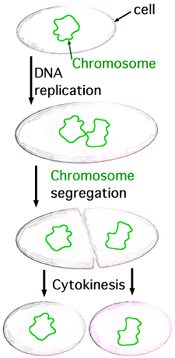
\includegraphics[width=.25\textwidth]{figs_steph/Binary_fission}
\end{center}



\begin{definition}
Mitosis+Cytokinesis: Mitosis is the process by which a cell separates its duplicated genome into two identical halves. It is generally followed immediately by cytokinesis which divides the cytoplasm and cell membrane. This results in two identical daughter cells with a roughly equal distribution of organelles and other cellular components. Mitosis and cytokinesis together is defined as the mitotic (M) phase of the cell cycle, the division of the mother cell into two daughter cells, each the genetic equivalent of the parent cell.
\end{definition}
\begin{center}
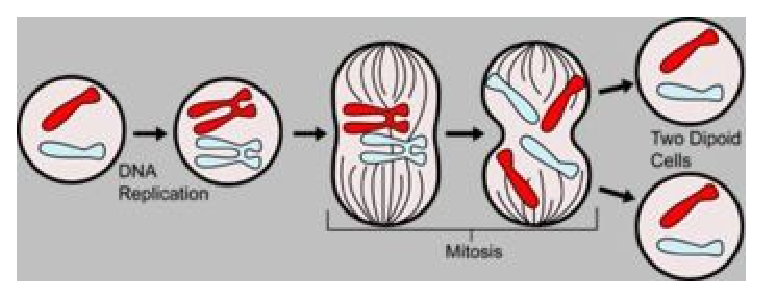
\includegraphics[width=.8\textwidth]{figs_steph/Mitosis}
\end{center}

Organisms that reproduce by binary fission (asexual reproduction) exhibit exponential growth. If organisms (or cells) are synchronized, the formalism of difference equation can be used.
The model (for an unlimited environment) to describe the temporal evolution of the E. Coli colony is expressed as
$$x_{t+1}=2x_t, \quad t=0,1,2,\dots$$
where $x_t$ is the state variable that represents the number of cells at the generation $t$. If the initial population $x_0$ is known then the solution is unique and is 
$$x_{t}=2^tx_0, \quad t=0,1,2,\dots$$

The asymptotic behavior of the solution is
$$\lim_{t\rightarrow \infty} x_t=\infty$$
as $a=2>1$. 
Note: If differential equation formalism was used
$$\frac{dx}{dt}=\frac{1440}{20}x$$
the solution would be $x(t)=x_0e^{\frac{1440}{20}t}$.



\section{The Ricker model}
another model for describing a population $N(t)$ in a limited environment
$$N(t+1)=N(t)\exp\left\{r\left(1-\frac{N(t)}{K}\right) \right\}=f(N(t)),$$
where $r$ is the intrinsic growth rate and $K$ is the carrying capacity. The growth rate $f(N(t))$ is increasing  in $N(t)$ and the per capita growth $\frac{f(N)}{N}$ is decreasing in $N(t)$. The increase in population is not sufficient to compensate for the decrease in the per capita growth, then $\lim_{N(t)\rightarrow +\infty}f(N(t))=0$. Then the Ricker model can be referred as to overcompensatory.
\begin{itemize}
\item $r < 2$ Globally asymptotically stable equilibrium $\bar x=K$
\item r = 2 Bifurcation into a stable 2-cycle
\item r = 2.5 Bifurcation into a stable 4-cycle
\item Then there is a series of cycle duplication: 8-cycle, 16-cycle, etc.
\item r = 2.692 Chaos 
\item For $r > 2.7$ there are some regions where dynamics returns to a cycle, e.g., r=3.15. 
\end{itemize}



\section{The Hassell model}
A population $N(t)$ in a limited environment
$$N(t+1)=\frac{rN(t)}{(1 + N(t))^b}$$
where $r$ is the intrinsic growth rate for small populations and b represents the inhibitive density-dependent feedback, usually attributed to the environment. 



\section{The Beverton-Holt model}
$$N(t+1)=\frac{ e ^r K N(t)}{K + (e^r -1)N(t)}$$
with $r$ is the intrinsic growth rate, the carrying capacity is $K$.

\section{Example of a 2-dimensional system}
\begin{equation*}
\begin{array}{cl}
x(t+1)=&x(t)(a-x(t)-y(t)), \quad a>0\\
y(t+1)=&y(t)(b+x(t)), \quad 0<b<1.
\end{array}
\end{equation*}


To find equilibria, solve the fixed point problem for $x$ and $y$,
\begin{equation*}
\begin{array}{cl}
x=&x(a-x-y)\\
y=&y(b+x)
\end{array}
\end{equation*}
We find 3 equilibria:
\[
(\bar x_1, \bar y_1)=(0,0), \quad  (\bar x_2, \bar y_2)=(a-1,0), \quad (\bar x_3, \bar y_3)=(1-b,a+b-2).
\]
The Jacobian of the system is
\[
J=\begin{pmatrix}
a-2x-y & -x \\
y & b+x
\end{pmatrix}.
\]
The Jacobians evaluated at each equilibrium are:
$$
J_{(\bar x_1, \bar y_1)}=\left ( 
\begin{array}{cc}
a & 0 \\
0 & b
\end{array}
\right ) \quad 
J_{(\bar x_2, \bar y_2)}=\left ( 
\begin{array}{cc}
2-a & 1-a \\
0 & b+a-1
\end{array}
\right ) \quad
J_{(\bar x_3, \bar y_3)}=\left ( 
\begin{array}{cc}
b & -1+b \\
a+b-2 & 1
\end{array}
\right )
$$
\begin{itemize}
\item Eigenvalues of $J_{(\bar x_1, \bar y_1)}$ are $a$ and $b$. By definition $|b|<1$. If $a<1$, $(\bar x_1, \bar y_1)$ is L.A.S.
\item $(\bar x_2, \bar y_2)=(a-1,0)$ exists only if $1<a$. Eigenvalues of $J_{(\bar x_2, \bar y_2)}$ are $2-a$ and $b+a-1$, then the stability of $(\bar x_2, \bar y_2)$ depends on $|2-a|<1$ and $|b+a-1|<1$. These inequalities lead to $1<a<2-b$.
\item From Theorem \ref{theo:stable2dim}, $(\bar x_3, \bar y_3)$ is L.A.S. if 
$$|1+b|<1+b-(-1+b)(a+b-2)<2.$$
$(\bar x_3, \bar y_3)$ is positive if $b<1$ and $a+b>2$. Then the biological existence and the LAS of $(\bar x_3, \bar y_3)$ are possible for
$$2<a+b<3.$$
\end{itemize}


\section{An SIR epidemic model}
Epidemic models were introduced in Section~\ref{sec:epid_residence_time}, and will be further discussed in Chapter~\ref{chap:epidemic_models} (in the ODE case). We refer in particular to Chapter~\ref{chap:epidemic_models}, where much more details can be found.

Here, we present an example of SIR model in difference equation formalism.
\begin{figure}[h]
%\includegraphics[width=0.8\textwidth]{figs_steph/SIR}
\caption{SIR model: disease with recovery and permanent immunity, here birth=death=b.}
\end{figure}
\begin{align}
S(t+1) &= S(t)-\beta \dfrac{S(t)}{N}I(t) +b(I(t)+R(t))\\
I(t+1) &= (1-\gamma -b)I(t)+\beta \dfrac{S(t)}{N}I(t)\\
R(t+1) &= R(t)(1-b)+\gamma I(t),
\end{align}
where $N=S(0)+I(0)+R(0)$. Parameters are $\beta$, the contact number (the average number of successful contacts made by one infected individual during the time $t$ to $t+1$), $b=d$, the rate of birth and death, $\gamma$, the rate of recovery ($1/\gamma $ is the average length of the infectious period when there are no death, $1/(\gamma +b)$ is the average length of the infectious period when deaths are included).

It is easy to check that the total population is constant, $N=S(t)+I(t)+R(t)$.
Also, solutions are nonnegative if $b,\gamma>0$ and
$$0<b+\gamma <1, \qquad 0<\beta <1$$.

We now consider the reduced system where $R(t)=N-I(t)-S(t)$ (which can be done since the total population is constant):
\begin{align*}
S(t+1)&=S(t)-\beta \dfrac{S(t)}{N}I(t) +b(N-S(t))\\
I(t+1)&=(1-\gamma -b)I(t)+\beta \dfrac{S(t)}{N}I(t).
\end{align*}
We find two equilibria: the disease-free equilibrium $(S_1,I_1)=(N,0)$ and the endemic equilibrium $(S_2,I_2)=\left (N\frac{(\gamma+b)}{\beta},bN\frac{\beta - (\gamma + b)}{\beta (\gamma +b)}\right)$.

\subsection{Stability of the disease free equilibrium $(S_1,I_1)$}
The Jacobian evaluated at $(S_1,I_1)$ is
$$
J(S_1,I_1)=\left (
\begin{array}{cc}
1-b & -\beta \\
0 & 1-b-\gamma +\beta 
\end{array}
\right )
$$
as the Jacobian is upper triangular its eigenvalues are
$$\lambda _1 = 1-b , \quad \lambda _2= 1-b-\gamma +\beta  .$$
$(S_1,I_1)$ is locally asymptotically stable if $|\lambda_{1,2}|<1$
\begin{itemize}
\item from assumptions, we have $0<\lambda _1 <1$
\item if $\frac{\beta}{\gamma +b}<1$ (where $\mathcal{R}_0=\frac{\beta}{\gamma +b}$ is the basis reproduction number), $0<\lambda _2 <1$
\end{itemize}
if $\mathcal{R}_0 <1$, there exist only one (biologically plausible) equilibrium, the disease-free equilibrium, and it is L.A.S. (see Figure \ref{fig:SIRsimul})


\subsection{Stability of the endemic equilibrium $(S_2,I_2)$}
The Jacobian evaluated at $(S_2,I_2)$ is
$$
J(S_2,I_2)=\left (
\begin{array}{cc}
1-b\mathcal{R}_0 & -\beta/\mathcal{R}_0 \\
b(\mathcal{R}_0-1) & 1
\end{array}
\right )
$$
where $\tr(J(S_2,I_2))=2-b\mathcal{R}_0 $ (assume $ \tr(J(S_2,I_2))\geq 0$), and $\det(J(S_2,I_2))=1-b\mathcal{R}_0+\beta b (1-\frac{1}{\mathcal{R}_0})$.


Condition for L.A.S (Theorem \ref{theo:stable2dim})
$$2-b\mathcal{R}_0 <2-b\mathcal{R}_0+\beta b (1-\frac{1}{\mathcal{R}_0}) <2$$
this condition is satified because
$$\beta (1-1/\mathcal{R}_0)<1<\mathcal{R}_0$$

If $1<\mathcal{R_0}\leq 2/b$, the endemic equilibrium  exists and it is L.A.S. (see Figure \ref{fig:SIRsimul}).

%\begin{figure}[h]
%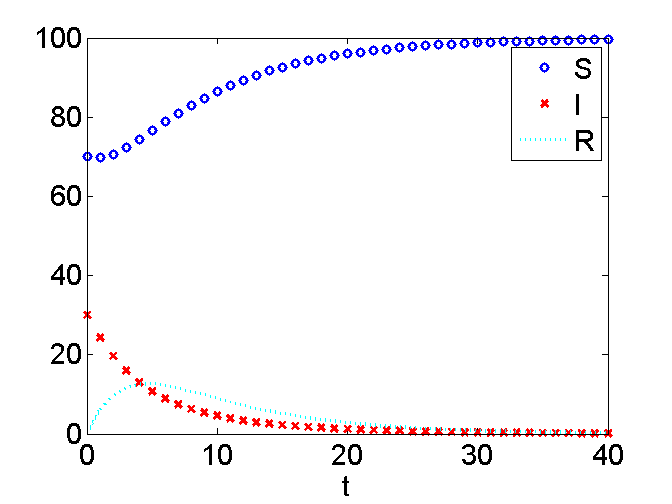
\includegraphics[width=.49\textwidth]{figs_steph/R1}
%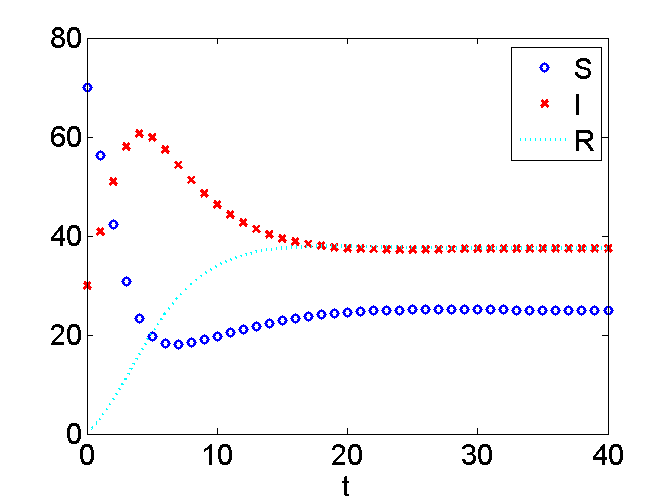
\includegraphics[width=.49\textwidth]{figs_steph/R4}
%\label{fig:SIRsimul}
%\caption{SIR model: {\bf Left)} $R_0=0.75$ the disease-free equilibrium is L.A.S. {\bf Right)} $R_0=4$ the endemic equilibrium is L.A.S}
%\end{figure}


\section{Predator-Prey models}
{\bf Assumptions}
\begin{itemize}
\item the prey has unlimited resources
\item the prey's only threat is the predator
\item the predator is a specialist; i.e., the predator's only food supply is the prey
\item predator growth depends on the prey it catches
\end{itemize}
{\bf Variables}
\begin{itemize}
\item $N(t)$ number of preys
\item $P(t)$ number of predators
\end{itemize}
{\bf Parameters}
\begin{itemize}
\item $r$ intrinsic rate of growth of prey
\item $d$ rate of death of predators
\item $eP(t)$ per capita prey reduction due to predation
\item $bN(t)$ per capita predator increase due to prey
\end{itemize}
\begin{equation*}
\begin{array}{cl}
N(t+1)=&(1+r)N(t)-e N(t)P(t)\\
P(t+1)=&(1-d)P(t)+bN(t)P(t)
\end{array}
\end{equation*}

{\bf Neubert and Kot model:}
If the prey follows a logistic growth
\begin{equation*}
\begin{array}{cl}
N(t+1)=&N(t)+rN(t)\left ( 1-\frac{N(t)}{K} \right ) -e N(t)P(t)\\
P(t+1)=&(1-d)P(t)+bN(t)P(t)
\end{array}
\end{equation*}




\section{Structured population models}
Structured population models are used when the population can be organized or divided into various subclasses following traits such as age, life-stage or size. The variable that describes this trait is called the structuring variable.
\begin{itemize}
\item In age-structured model, the  population is subdivided into age groups. For the human population, for example, age groups may be 5 year lengths, 0-5, 5-10, $\dots$, or 1 year lengths.
\item In stage-structured model, the population is organized into developmental stage: juveniles and adults, or for insects, egg, larva, pupa and adult.
\item In size-structured  model, individuals in the population are grouped according to size (length, weight, biomass).
\end{itemize}
The dynamic interactions among the stages, ages or sizes determine how the population structure changes over the time. Other structuring variables can be taken into account: sex and space.




\section{Leslie matrix model}
The Leslie Matrix (also called the Leslie Model) describes the growth of populations with structure (and their projected age distribution); the population is closed to migration and only one sex, usually the female, is considered.


Assume the population is closed to migration and only the females are modeled. Males are presented, but are not specifically modeled (when the sex ratio of males to females is $a/b$ and the survival rate per age group is the same for males and females, then the number of males equals the number of females times $a/b$). 


Let the total number of age groups is $m$ ($m$ the last reproductive age). During the interval of time $t$ and $t+1$ individuals age from $i$ to $i+1$: time interval coincides with the age interval.
\begin{itemize}
\item $x_i(t)$ number of females in the $i^{th}$ age group at time $t$.
\item $b_i$ average number of newborn females produced by one females in the $i^{th}$ age group that survive through the time interval in which they were born, $b_i\geq 0$
\item $s_i$ fraction of the $i^{th}$ age group that lives  to the $(i+1)st$ age, $0<s_i\leq 1$
\end{itemize}
\begin{figure}
\begin{center}
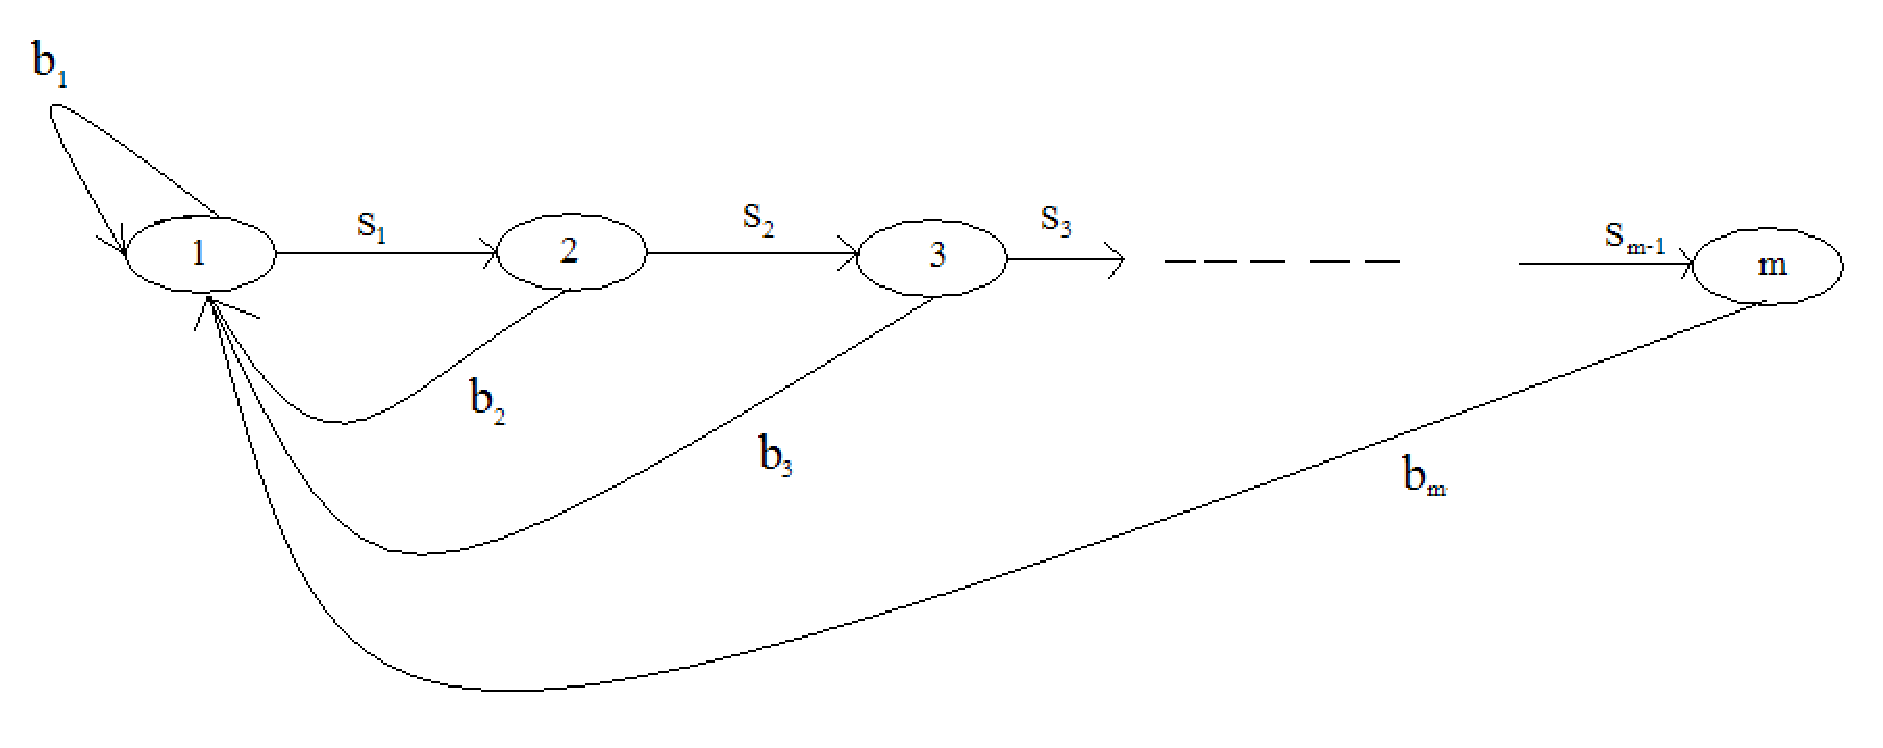
\includegraphics[width=0.6\textwidth]{figs_steph/LesliePattern}
\caption{Life cycle graph of the Leslie matrix on $m$ age classes: each node represents each age group $x_i$, and arcs represent relation between two groups. An arrow connects the node $j$ to $i$ if the $ij^{th}$ element in the Leslie matrix $L$ is nonzero.}
\end{center}
\end{figure}

\begin{subequations} 
\begin{align}
x_{1}(t+1)=& b_1 x_1(t)+b_2x_2(t)+b_3x_3(t)+\dots b_mx_m(t)\label{eq:Leslie1}\\
x_{2}(t+1)=&s_1 x_1(t)& \label{eq:Leslie2}\\
x_{3}(t+1)=&s_2 x_2(t)& \label{eq:Leslie3}\\
\vdots &\\
x_{m}(t+1)=&s_{m-1} x_{m-1}(t)& \label{eq:Leslie3}\\
\end{align}   
\end{subequations} 
Using matrix notation,
\begin{equation}
X(t+1)=\left (
\begin{array}{c}
x_1(t+1)\\
x_2(t+1)\\
x_3(t+1)\\
\vdots\\
x_m(t+1)
\end{array}
\right )
=
\left(
\begin{array}{ccccc}
b_1 & b_2 & \hdots & b_{m-1} & b_m\\
s_1 & 0  & \hdots & 0 & 0\\
0 & s_2  & \hdots & 0 & 0\\
\vdots & \vdots & \ddots & \vdots & \vdots \\
0 &0 &\hdots & s_{m-1} &0
\end{array}
\right)
\left (
\begin{array}{c}
x_1(t)\\
x_2(t)\\
x_3(t)\\
\vdots\\
x_m(t)
\end{array}
\right )=LX(t)
\end{equation}
where $L$ is called the Leslie matrix: fertilities or fecundities on the first row and survival probabilities on the subdiagonal. All other entries in the Leslie matrix are zero.



$$X(1)=LX(0)$$
$$X(2)=LX(1)=L\left(LX(0)\right)=L^2X(0)$$
In general
$$X(t)=L^tX(0)$$







\begin{definition}
A Leslie matrix is a nonnegative matrix.
\end{definition}




A necessary condition for a Leslie matrix to be irreductible is $b_m\not =0$.


Frobenius Theorem gives sufficient conditions that guarantees the Leslie matrix has one positive strictly dominant eigenvalue.


If the Leslie matrix satisfies $L^p>0$ for some positive integer $p$, then $L$ is primitive. Then, the Frobenius Theorem states that in this case L has a unique strictly dominant eigenvalue $\lambda _1$ satisfying $|\lambda _1|>|\lambda _i|$, for $j\not =1$, that is positive. Associated with the strictly dominant eigenvalue $\lambda _1$ is a positive eigenvector $V_1$, that is referred to as a stable age distribution.


Assume matrix $L$ is irreductible and primitive and $m$ eigenvectors form a linearly independent set; then the solution to
$$X(t+1)=LX(t)$$
can be written
$$X(t)=L^tX(0)=\sum_{i=1}^m c_i \lambda _i ^t V_i$$
where $\lambda _1$ is the strictly dominant eigenvalue. Dividing the solution by $\lambda _1^t$ gives
$$\frac{X(t)}{\lambda _1^t}=\frac{L^tX(0)}{\lambda _1^t}=c_1 V_1 + \frac{c_2 \lambda _2 ^t}{\lambda _1^t} V_2+\dots + \frac{c_m \lambda _m ^t}{\lambda _1^t} V_m $$
As $|\lambda _i/\lambda_1|<1$, $(\lambda _i/\lambda_1)^t\rightarrow 0$ as $t\rightarrow +\infty$. Thus
$$\lim_{t\rightarrow +\infty} \frac{X(t)}{\lambda _1^t}=\lim_{t\rightarrow +\infty}  \frac{L^tX(0)}{\lambda _1^t}=c_1V_1 .$$
Hence after many generations, $X(t)=L^tX(0)=c_1\lambda _1^tV_1$. The population size either increasing ($\lambda _1 >1$) or decreasing ($\lambda _1 <1$) geometrically as $t$ goes larger.

The population distribution $X(t)/\lambda _1 ^t$ approaches a constant multiple of the eigenvector $V_1$; thus $V_1$ is referred to as a stable age distribution. It means that for large values of time, the age distribution vector is a scalar multiple of the eigenvector associated with the largest eigenvalue of the matrix. Consequently the proportion of females in each of the age classes becomes constant, these limiting proportions can be determined from the eigenvector $V_1$.

An explicit expression for $V_1$ in the case of a Leslie matrix is \cite{Pielou1977}
\begin{equation}
\label{eq:Eigenvector}
V_1=\left (\begin{array}{c}
1\\
\frac{s_1}{\lambda _1}\\
\vdots\\
\frac{s_1s_2\dots s_{m-2}}{\lambda_1^{m-2}}\\
\frac{s_1s_2\dots s_{m-1}}{\lambda_1^{m-1}}
\end{array}\right )
\end{equation}


The characteristic equation for the Leslie matrix satisfies $\det(L-\lambda I)=0$ or
$$\det 
\left(
\begin{array}{ccccc}
b_1-\lambda & b_2 & \hdots & b_{m-1} & b_m\\
s_1 & -\lambda  & \hdots & 0 & 0\\
0 & s_2  & \hdots & 0 & 0\\
\vdots & \vdots & \ddots & \vdots & \vdots \\
0 &0 &\hdots & s_{m-1} &-\lambda
\end{array}
\right)=0$$
or
$$p(\lambda)=\lambda ^m-b_1 \lambda^{m-1}-b_2s_1 \lambda^{m-2}- b_3s_1 s_2 \lambda^{m-3}-\dots - b_m s_1s_2 s_3\dots s_{m-1}=0 $$
From Descarte's Rule, since there is only one change in sign in the polynomial, $p(\lambda)$ has one positive real root, that is the dominant eigenvalue $\lambda _1$.

How is the dominant eigenvalue $\lambda _1$: $\lambda _1 >1$ or $\lambda _1 <1$?
\begin{itemize}
\item $\lim _{\lambda \rightarrow \infty}p(\lambda)=\infty$
\item $p(0)<0$
\item $p(\lambda)$ crosses the positive $\lambda-$axis only once at $\lambda_1$
\end{itemize}
then 
\begin{itemize}
\item $\lambda _1 >1$ $\Leftrightarrow$ $p(1)<0$
\item $\lambda _1 <1$ $\Leftrightarrow$ $p(1)>0$
\end{itemize}
where $p(1)=1-b_1 -b_2s_1 - b_3s_1 s_2 -\dots - b_m s_1s_2 s_3\dots s_{m-1}$, and $p(1)=1-R_0$.
Hence
\begin{itemize}
\item $\lambda _1 >1$ $\Leftrightarrow$ $1<R_0$
\item $\lambda _1 <1$ $\Leftrightarrow$ $1>R_0$
\end{itemize}

\begin{definition}
The reproductive number $R_0$ is the average number of offspring produced by an
individual in its lifetime:
$$R_0=b_1+b_2s_1+b_3s_1s_2+\dots+b_ms_1s_2\dots s_{m-1}$$
where each term represent the average
number of offsprings produced by individuals of age $i$.
\begin{itemize}
\item $R_0 < 1$ individuals not fully replacing themselves, population shrinking
\item $R_0 = 1$ individual exactly replacing themselves, population size stable
\item $R_0 > 1$ individuals more than replacing themselves, population growing
\end{itemize}
\end{definition}


\begin{theorem}
Assume the Leslie matrix $L$ defined as
$$X(t+1)=\left (
\begin{array}{c}
x_1(t+1)\\
x_2(t+1)\\
x_3(t+1)\\
\vdots\\
x_m(t+1)
\end{array}
\right )
=
\left(
\begin{array}{ccccc}
b_1 & b_2 & \hdots & b_{m-1} & b_m\\
s_1 & 0  & \hdots & 0 & 0\\
0 & s_2  & \hdots & 0 & 0\\
\vdots & \vdots & \ddots & \vdots & \vdots \\
0 &0 &\hdots & s_{m-1} &0
\end{array}
\right)
\left (
\begin{array}{c}
x_1(t)\\
x_2(t)\\
x_3(t)\\
\vdots\\
x_m(t)
\end{array}
\right )=LX(t)
$$
is irreductible and primitive. The characteristic polynomial of $L$ i given by
$$p(\lambda)=\lambda ^m-b_1 \lambda^{m-1}-b_2s_1 \lambda^{m-2}- b_3s_1 s_2 \lambda^{m-3}-\dots - b_m s_1s_2 s_3\dots s_{m-1}=0 .$$
Matrix $L$ has a strictly dominant eigenvalue $\lambda _1>0$ satisfying the following relationships:
\begin{itemize}
\item $\lambda _1 =1$ if and only if $R_0=1$,
\item $\lambda _1 <1$ if and only if $R_0<1$,
\item $\lambda _1 >1$ if and only if $R_0>1$,
\end{itemize}
where $R_0$ is the inherent reproductive number defined by
$$R_0=b_1+b_2s_1+b_3s_1s_2+\dots+b_ms_1s_2\dots s_{m-1}.$$
In addition the stable age distribution $V_1$ satisfies
$$V_1=\left (\begin{array}{c}
1\\
\frac{s_1}{\lambda _1}\\
\vdots\\
\frac{s_1s_2\dots s_{m-2}}{\lambda_1^{m-2}}\\
\frac{s_1s_2\dots s_{m-1}}{\lambda_1^{m-1}}
\end{array}\right ).
$$
\end{theorem}

\subsection{Salmon population}
Suppose a population of salmon live to three years of age. Each adult salmon produces 800 offspring. The
probability of a salmon surviving the first year to live on to the second year is $5\%$, and the probability of a
salmon surviving the second year to live on to the third year is $2.5\%$.
\begin{itemize}
\item Find the Leslie matrix for this population.
\item If there are 10 females in each of the three age classes, find the initial age distribution vector. Use Matlab
to find the population age distribution vectors for each of the first 100 years.
\item Use Matlab to find the eigenvalues and eigenvectors of the Leslie Matrix. Is there a strictly dominant eigenvalue?
\item Describe what happens to this population of salmon over time?
\end{itemize}

\subsection{Human Population}
Suppose the population of the United States is broken up into ten 5-year age classes. The values for the
reproduction rates $F_i$ and the survival rates $P_i$ for each age class are shown in the table below.


\begin{tabular}{ccc}
i &$F_i$ & $P_i$\\
1 & 0 & 0.99670\\
2 &0.00102 &0.99837\\
3 &0.08515 &0.99780\\
4 &0.30574 &0.99672\\
5 &0.40002 &0.99607\\
6 &0.28061 &0.99472\\
7 &0.15260 &0.99240\\
8 &0.06420 &0.98867\\
9 &0.01483 &0.98274\\
10 &0.00089 &0
\end{tabular}
\begin{itemize}
\item Find the Leslie matrix for this population.
\item  If there are 10 females in each of the ten age classes, find the initial age distribution vector. Use Matlab to
find the population age distribution vectors for each of the first 100 years, and plot the age distribution
vectors.
\item  Use Matlab to find the eigenvalues and eigenvectors of the Leslie Matrix. What happens to this population
over time?
\item  After a long period of time, what is the relative number of females in each of the ten age classes?
%\item  After a long period of time, by what percentage is the population growing or shrinking?
\end{itemize}

\subsection{Insect population}
Insect Life cycle:
\begin{description}
\item[ADULT] 
The life cycle description can be started with the adult insect. The adult may be a beetle, fly, moth, or midge. Regardless of their form, insects mate and most lay eggs.
\item[EGG] 
Eggs come in many shapes, sizes, and colors. They might be deposited on or in the ground, the roots, the stems, the leaves, or the flowers. When the eggs hatch the new insect is called a larva. 
\item[LARVA]
The larva seldom looks like the adult it will become. Some common larval forms are the maggot, grub worm, inchworm, and caterpillar. As the larva grows it must shed it�s old skin from time to time. This is called molting. From hatching to the first molt the larva is said to be in it�s 1st instar stage. After molting the first time the larva enters it�s second instar stage, and so on. The feeding activity of the larvae often inflicts more damage on the noxious weed than the adult form. Different insects have different numbers of instars, but eventually the larva is fully grown and ready to pupate.
\item[PUPA] 
The pupa is the life stage between larva and adult. In this stage the insect does not feed, and can be considered motionless. This metamorphic change is often profound. Unless the larva is in a stem or root tunnel it will usually construct some kind of shelter to pupate in. This "cocoon" might be made from soil particles, silk, chewed seeds, chewed plant material, ground litter, or combinations.
Inside the "cocoon/shelter/chamber/capsule/case" the pupa is gradually transformed into an adult.
\end{description}
\begin{figure}
\begin{center}
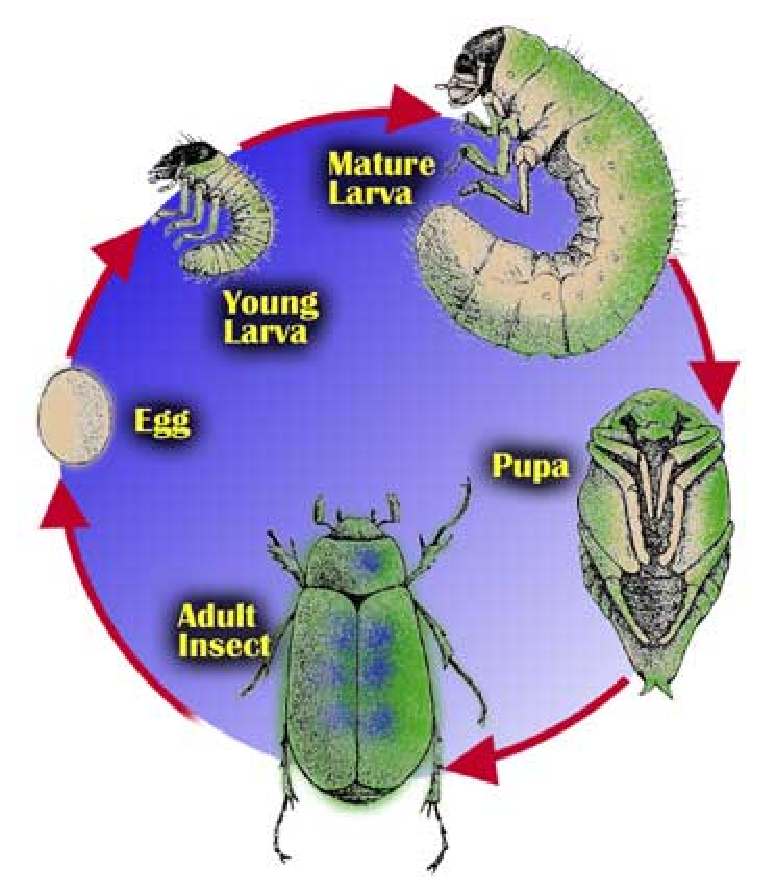
\includegraphics[width=.4\textwidth]{figs_steph/insect_life_cycle}
\caption{Example of insect life cycle.}
\end{center}
\end{figure}



\section{Examples}

\subsection{Insect populations}
Assume that adult females of a species produce offspring at a fixed period of time each year. A proportion of the offspring (juveniles) survives to adulhood, reproduces, and dies (nonoverlapping of generations). Let
\begin{itemize}
\item $j_t$ number of juveniles in years $t$
\item $a_t$ number of adult females in year $t$
\item $p$ number of juveniles that survive in year $t$
\item $f$ number of offspring produced per female
\item $r$ ratio of females to adults.
\end{itemize}
Using the definition of state variables and parameters given above, the model can be expressed as follows
$$a_{t+1}=prj_t$$
$$j_{t+1}=f a_{t+1}$$
The system can be condensed in an unique equation:
$$j_{t+1}=f prj_t$$
If the initial population $j_0$ of juveniles is known, the solution is unique and is
$$j_t=(f pr)^tj_0 \quad t=0,1,2,\dots$$
The asymptotic behavior of the solution depends on the value of $f pr$:
\begin{itemize}
\item If $f pr<1$ $\lim_{t\rightarrow +\infty} j_t=0$ extinction of the population,
\item If $f pr>1$ $\lim_{t\rightarrow +\infty} j_t=+\infty$ explosion of the population.
\end{itemize}
\subsection{Pharmacology}
A drug is administred once every four hours. Let $D_n$ be the amount of the drug in the blood system at the $n^{th}$ interval.  The body eliminates a certain fraction $p$ of the drug during each time interval. If the amount administred is $D_0$, find $D_n$ and $\lim _{n \rightarrow}D_{n}$.

$$D_{n+1}=D_n-pD_n +D_0=(1-p)D_n +D_0 \quad n=0,1,\dots$$
and the initial condition is $D_0$.

The equilibrium solution is $D^*=\frac{D_0}{p}$ (obtained by solving $D_{n}=(1-p)D_n +D_0$)
 
Using Proposition \ref{Prop:FirstLinNonH} the solution is unique and is
$$D_n=(1-p)^n\left [D_0-\frac{D_0}{p}\right ] +\frac{D_0}{p} \quad n=0,1,2,\quad$$

Limiting behavior is
$$\lim _{n\rightarrow +\infty}D_n=\frac{D_0}{p}$$
as $(1-p)<1$.

\begin{quote}
Note: If differential equation formalism was used
$$\frac{dD}{dt}=-pD +D_0, \quad D(0)=D_0$$
the solution would be $D(t)=\frac{D_0}{p}+(D_0-\frac{D_0}{p})e^{-pt}$.
\end{quote}


\subsection{Propagation of annual plants}
Plants produce seeds at the end of their growth season (August), after which they die. A fraction of these seeds survive the winter, and some of these germinate at the beginning of the season (May), giving rise to the new generation of plants. The fraction that germinates depends on the age of the seeds. 
\begin{itemize}
\item $\gamma$ number of seeds produced per plant in August
\item $\sigma$ fraction of seeds that survive a given winter
\item $\alpha$ fraction of one-year-old seeds that germinate in May
\item $\beta$ fraction of two-year-old seeds that germinate in May
\item Seeds older than two years are no longer viable
\end{itemize}

State variables:
\begin{itemize}
\item $p_n$ number of plants in generation $n$
\item $s_n$ number of new seed in generation $n$
\item $s^1_n$ number of one-year-old seeds in generation $n$
\item $s_{n}^{2}$ number of two-year-old seeds in generation $n$
\end{itemize}
Equations:
\begin{subequations}\label{eq:plant}
\begin{align}
p_n=&\alpha s^1_n+\beta s_{n}^{2}\label{eq:plant1}\\
s_{n}=&\gamma p_{n}\label{eq:plant2}\\
s_n^1=&\sigma s_{n-1}\label{eq:plant3}\\
s_{n}^{2}=&\sigma (1-\alpha)s^1_{n-1}\label{eq:plant4}
\end{align}   
\end{subequations} 
Condensing equations \eqref{eq:plant2}, \eqref{eq:plant3} and \eqref{eq:plant4} we obtain
$$s_n^1=\sigma \gamma p_{n-1}$$
and 
$$s_{n}^{2}=\sigma (1-\alpha)\sigma \gamma p_{n-2}$$
therefore, we can express the model as a system of 3 First-order difference equations
\begin{equation*}
\begin{array}{ll}
p_n=&\alpha s_n+\beta \sigma (1-\alpha)s_{n-1}\\
s_n^1=&\sigma \gamma p_{n-1}\\
s_{n}^{2}=&\sigma (1-\alpha)\sigma \gamma p_{n-2}
\end{array}
\end{equation*}
or as 1 Second-order equation:
\begin{equation}\label{eq:PLANTS}
p_n=\alpha \sigma \gamma p_{n-1}+\beta \sigma (1-\alpha)\sigma \gamma p_{n-2}
\end{equation}

Characteristic equation corresponding to the model \eqref{eq:PLANTS} is
$$\lambda ^2 - \alpha \sigma \gamma \lambda - \beta \sigma^2 (1-\alpha) \gamma=0$$

Eigenvalues are
$$\lambda _{1,2}=\frac{\alpha \sigma \gamma \pm \sqrt{(\alpha \sigma \gamma)^2+4\beta \sigma^2 (1-\alpha) \gamma}}{2}$$

%=\frac{\alpha \sigma \gamma \pm \sigma\sqrt{(\alpha  \gamma)^2+4\beta  (1-\alpha) \gamma}}{2}

$$\lambda _{1,2}=\frac{\alpha \sigma \gamma }{2}\left (1\pm \sqrt{1+\frac{4\beta  (1-\alpha)}{\alpha^2 \gamma }}\right )$$
%where $\delta = \frac{4\beta  (1-\alpha)}{\alpha^2 \gamma }$

The dominating eigenvalue (the eigenvalue corresponding to the solution that determines the limiting behavior of the general solution) is the positive eigenvalue
$$\lambda _{1}=\frac{\alpha \sigma \gamma }{2}\left (1+ \sqrt{1+\frac{4\beta  (1-\alpha)}{\alpha^2 \gamma }}\right )$$

If $0<\lambda _1 <1$ the plant population will extinct.
If $\lambda _1 >1$ the plant population will grow.






\subsection{Red blood cell}
In the circulatory system, red blood cells are constantly being destroyed and replaced. They carry oxygen throughout the body and they must be maintained at a constant level. The spleen filters out and destroys a fraction of the cells daily and the bone marrow produces a number proportional to the number lost on the previous day. The cell count on dat $t$ is modeled as followed:
\begin{itemize}
\item $R_t$ number of red blood cells in circulation on day $t$.
\item $M_t$ number of red blood cells produced by marrow on day $t$.
\item $f$ fraction of red blood cells removed by spleen, $0<f<1$.
\item $\gamma$ production constant, $\gamma >0$
\end{itemize}
The system of difference equations is
\begin{subequations}\label{eq:reblood}
\begin{align}
R_{t+1}=&(1-f)R_t+M_t\label{eq:reblood1}\\
M_{t+1}=&\gamma f R_t \label{eq:reblood2}
\end{align}   
\end{subequations} 
or a Second-order difference equation:
\begin{equation}\label{eq:BLOOD}
R_{t+1}=(1-f)R_t+\gamma f R_{t-1}
\end{equation}
Characteristic equation corresponding to the model \eqref{eq:BLOOD} is
$$\lambda ^2 - (1-f) \lambda -  \gamma f=0$$
Eignevalues are
$$\lambda_{1,2}=\frac{(1-f)\pm \sqrt{(1-f)^2 + 4 \gamma f}}{2}$$

For homeostasis in the red blood cell count, the total number of red blood cell has to stay constant. Then the dominanting eigenvalue has to be $\lambda_1 =1$.

The dominating eigenvalue is 
$$\lambda_{1}=\frac{(1-f)+ \sqrt{(1-f)^2 + 4 \gamma f}}{2}.$$
By investigating $\lambda _1= 1$, we found that the condition, $\gamma =1$, has to be satisfied.


If $\gamma =1$, $\lambda _2= -f$, and the solution is
$$R_t= c_1 (-f^{t}) +c_2$$
the system is oscillating but decreasing in magnitude to reach a constant number.



\subsection{Structured model}

%Stage-structured models have been frequently applied to fish population.
\subsubsection{Killer whales}
Killer whales are long-lived marine mammals that live in stable
social groups called ``pods''. Demographic
data on killer whale populations in the coastal waters of British Columbia and Washington
state have been collected since 1973. Brault and Caswell (1993) used the 1973-1987 data and
a stage-structured matrix model to investigated several demographic questions concerning the
whales. They model the females with a mixed age-stage classification: yearlings, juveniles (past
the first year, but not mature), mature females, and post-reproductive females. 
$$
A =\left (\begin{array}{cccc}
0 & 0.0043 & 0.1132 & 0\\
0.9775 & 0.9111 & 0 & 0\\
0 & 0.0736 & 0.9534 & 0\\
0 & 0 & 0.0452 & 0.9804
\end{array}\right )$$
\begin{itemize}
\item Draw the life-cycle graph associated with the matrix A.
\item Computes the dominant eigenvalue. 
\item Find the stable stage distribution for the whale population.
\item Projects the population dynamics for the next 50 years assuming that the current population
vector is $x_0 = (10, 60, 110, 70)$ .
%(c) Plots on 3 separate graphs the projected changes over time in
%(i) N(t) = total population size in year t,
%(ii) the annual population growth rate .(t) = N(t + 1)/N(t),
%(iii) the proportion of individuals in each stage.
%Does the population structure become stable? How does it change over time? How quickly
%does the annual growth rate .(t) converge to the dominant eigenvalue .?
\end{itemize}

MatLab code:
\begin{verbatim}
L=[0 0.0043 0.1123 0;.9775 0.9111 0 0;0 .0736 0.9534 0;0 0 0.0452 0.9804];
x0=[10;60;110;70];
X=zeros(4,51);
X(:,1)=x0;
%simulations
for k=2:51, X(:,k)=L*X(:,k-1); end
t=0:50;
plot(t,X);
xlabel('Time');
ylabel('Population');
legend('Yearlings', 'Juveniles', 'Mature females','Post-reproductive females')
% limiting behavior
L=[0 0.0043 0.1123 0;.9775 0.9111 0 0;0 .0736 0.9534 0;0 0 0.0452 0.9804];
Value=eig(L);
dominating=max(Value)
[V,D]=eig(L)
\end{verbatim}

\begin{verbatim}
dominating =
    1.0251

V =
         0    0.0658   -0.0655    0.6788
         0    0.5640    0.8371   -0.7321
         0    0.5789   -0.5187    0.0568
    1.0000    0.5852    0.1609   -0.0026

D =
    0.9804         0         0         0
         0    1.0251         0         0
         0         0    0.8346         0
         0         0         0    0.0048
         
>> v1=V(:,2)/sum(V(:,2))

v1 =
    0.0367
    0.3144
    0.3227
    0.3262         
\end{verbatim}

The dominant eigenvalue is $1.0251$, and the associated eigenvector is $(0.0658,0.5640,0.5789,0.5852)$. By suming all the entries of this eigenvector and by dividing each of its entries by this sum, we can express the stable stage distribution $v_1$ for the whale population.

\begin{center}
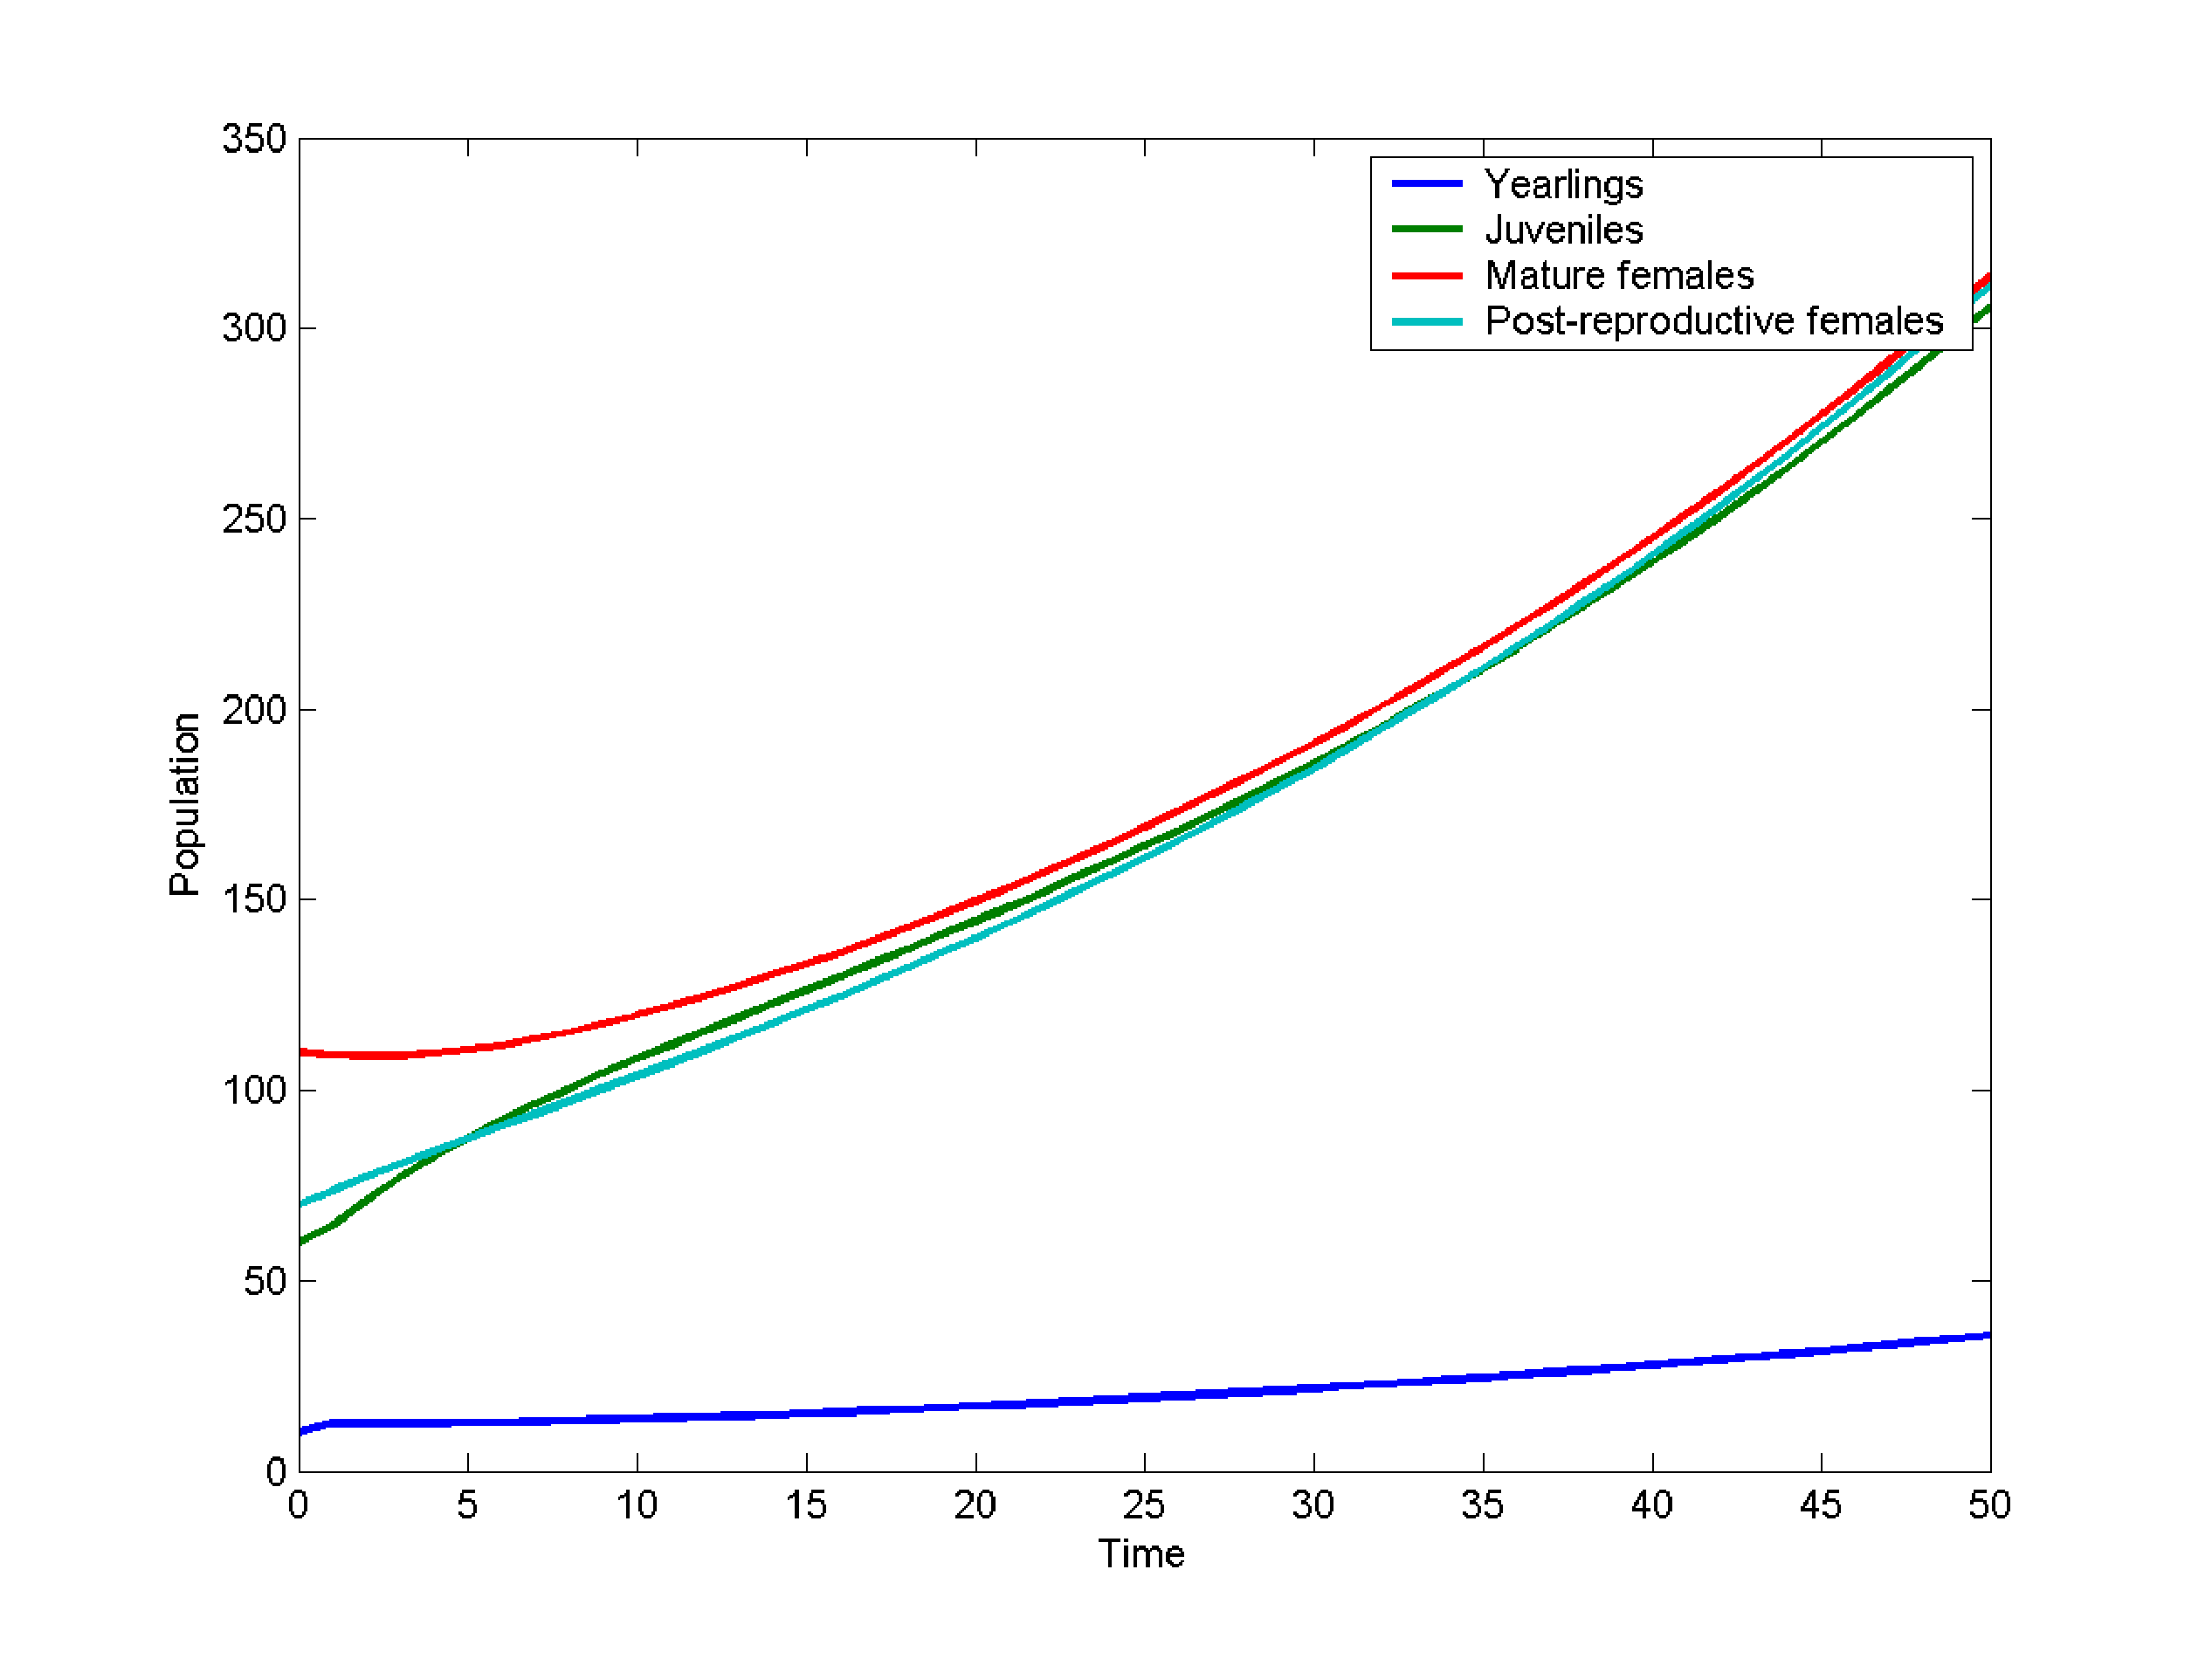
\includegraphics[width=.6\textwidth]{figs_steph/KillerWhales}
\end{center}
















\part{Markov chains}
\chapter{A brief theory of Markov chains}
\label{chap:markov}

\section{Markov chains}
We conduct an experiment with a set of $r$ outcomes,
\[
S=\{S_1,\dots, S_r\}.
\]
The experiment is repeated $n$ times (with $n$ large, potentially infinite). 
The system has no memory: the next state depends only on the present state. 
The probability of $S_j$ occurring on the next step, given that $S_i$ occurred on the last step, is
\[
p_{ij}=p(S_j|S_i).
\]
Suppose that $S_i$ is the current state, then one of $S_1, \ldots,S_r$ must be the next state; therefore,
\[
p_{i1}+p_{i2}+\cdots+p_{ir}=1, \quad 1\leq i\leq r.
\]
(Note that some of the $p_{ij}$ can be zero, all that is needed is that $\sum_{j=1}^r p_{ij}=1$ for all $i$.)

\begin{definition}
An experiment with finite number of possible outcomes $S_1,\ldots,S_r$ is repeated. The sequence of outcomes is a \emph{Markov chain} if there is a set of $r^2$ numbers $\{p_{ij}\}$ such that the conditional probability of outcome $S_j$ on any experiment given outcome $S_i$ on the previous experiment is $p_{ij}$, i.e., for $1\leq i,j\leq r$, $n=1,\ldots$,
\[
p_{ij}=\mathsf{Pr}(S_j\textrm{ on experiment }n+1|S_i\textrm{ on experiment }n).
\]
The outcomes $S_1,\ldots,S_r$ are the \emph{states}, and the $p_{ij}$ are the \emph{transition probabilities}. The matrix $P=[p_{ij}]$ is the \emph{transition matrix}.
\end{definition}
The matrix 
\[
P=
\begin{pmatrix}
p_{11} & p_{12} & \cdots & p_{1r} \\
p_{21} & p_{22} & \cdots & p_{2r} \\
&&& \\
p_{r1} & p_{r2} & \cdots & p_{rr}
\end{pmatrix}
\]
is called the \emph{transition matrix} of the Markov chain. It has
\begin{itemize}
\item nonnegative entries, $p_{ij}\geq 0$
\item entries less than 1, $p_{ij}\leq 1$
\item row sum 1, which we write
\[
\sum_{j=1}^r p_{ij}=1,\quad i=1,\ldots,r
\]
or, using the notation $\nbOne^T=(1,\ldots,1)$,
\[
P\nbOne=\nbOne.
\]
\end{itemize}
These properties guarantee that the elements of the matrix $P$ describe probabilities.


\section{Repetition of the process}

Let $p_i(n)$ be the probability that the state $S_i$ will occur on the $n^{th}$ repetition of the experiment, $1\leq i\leq r$. 
Since one the states $S_i$ must occur on the $n^{th}$ repetition,
\[
p_1(n)+p_2(n)+\cdots+p_r(n)=1.
\]
Let $p_i(n+1)$ be the probability that state $S_i$, $1\leq i\leq r$, occurs on $(n+1)^{th}$ repetition of the experiment. 
There are $r$ ways to be in state $S_i$ at step $n+1$:
\begin{enumerate}
\item[1.] Step $n$ is $S_1$. Probability of getting $S_1$ on $n^{th}$ step is $p_1(n)$, and probability of having $S_i$ after $S_1$ is $p_{1i}$. Therefore, by multiplication principle, $P(S_i|S_1)=p_{1i}p_1(n)$. 
\item[2.] We get $S_2$ on step $n$ and $S_i$ on step $(n+1)$. Then $P(S_i|S_2)=p_{2i}p_2(n)$. 
\item[..]
\item[r.] Probability of occurrence of $S_i$ at step $n+1$ if $S_r$ at step $n$ is $P(S_i|S_r)=p_{ri}p_r(n)$.
\end{enumerate}
Therefore, $p_i(n+1)$ is sum of all these,
\begin{align*}
p_i(n+1) &= P(S_i|S_1)+\cdots+P(S_i|S_r) \\
&= p_{1i}p_1(n)+\cdots+p_{ri}p_r(n)
\end{align*}
Therefore,
\begin{equation}\label{eq:chain1}
\begin{aligned}
p_1(n+1) &= p_{11}p_1(n)+p_{21}p_2(n)+\dots+p_{r1}p_r(n) \\
& \vdots\\
p_k(n+1) &= p_{1k}p_1(n)+p_{2k}p_2(n)+\dots+p_{rk}p_r(n) \\
& \vdots\\
p_r(n+1) &= p_{1r}p_1(n)+p_{2r}p_2(n)+\dots+p_{rr}p_r(n)
\end{aligned}
\end{equation}
In matrix form
\begin{equation}
p(n+1)=p(n)P, \quad n=1,2,3,\dots
\end{equation}
where $p(n)=(p_1(n),p_{2}(n),\dots , p_r(n))$ is a (row) probability vector and $P=(p_{ij})$ is a $r\times r$ \emph{transition matrix},
\[
P=
\begin{pmatrix}
p_{11} & p_{12} & \cdots & p_{1r} \\
p_{21} & p_{22} & \cdots & p_{2r} \\
&&& \\
p_{r1} & p_{r2} & \cdots & p_{rr}
\end{pmatrix}
\]
So, what we have is
\[
(p_1(n+1),\ldots,p_r(n+1))=
(p_1(n),\ldots,p_r(n))
\begin{pmatrix}
p_{11} & p_{12} & \cdots & p_{1r} \\
p_{21} & p_{22} & \cdots & p_{2r} \\
&&& \\
p_{r1} & p_{r2} & \cdots & p_{rr}
\end{pmatrix}
\]
It is easy to check that this gives the same expression as \eqref{eq:chain1}.

\subsection{Long time behaviour}
Let $p(0)$ be the initial distribution (row) vector. Then
\begin{align*}
p(1) &= p(0)P \\
p(2) &= p(1)P\\
&= (p(0)P)P \\
&= p(0)P^2
\end{align*}
Iterating, we get that for any $n$,
\[
p(n)=p(0)P^n
\]
Therefore, 
\begin{equation}\label{eq:limit_Markov_chain}
\lim_{n\rightarrow +\infty}p(n)=\lim_{n\rightarrow +\infty}p(0)P^n=p(0)\lim_{n\rightarrow +\infty}P^n.
\end{equation}
So, to determine the long time behaviour of the Markov chain, it suffices to determine the limit of the $P^n$.


\subsection{Stochastic matrices}
One fundamental property of Markov chains is that the transition matrix $P$ has a very particular structure.
\begin{definition}[Stochastic matrix]
The nonnegative $r\times r$ matrix $M$ is a \emph{stochastic} matrix if $\sum_{j=1}^ra_{ij}=1$ for all $i=1,2,\dots, r$, i.e., the rows of $M$ all sum to 1.
\end{definition}
Note that a matrix that has column sums all equal to 1 is also called a stochastic matrix. Such a matrix arises if instead of representing transitions from rows to columns as we have done, transitions are represented from columns to rows. 
If it is needed to distinguish between matrices that are stochastic by rows or by columns, we say that, say, a matrix is a (row) stochastic matrix.

A matrix that that both rows and column sums equal to 1 is a \emph{doubly stochastic} matrix.
Stochastic matrices over $\IR_+$ form a \emph{group}. This means in particular that the following holds true.
\begin{theorem}
If $M,N$ are stochastic matrices, then $MN$ is a stochastic matrix.
\end{theorem}
This is particularly interesting, as it means that powers of a stochastic matrix are also stochastic:
\begin{theorem}
If $M$ is a stochastic matrix, then for any $k\in\IN$, $M^k$ is a stochastic matrix.
\end{theorem}
A stochastic matrix has the property that all its eigenvalues are contained in the unit disk of $\IC$.
\begin{theorem}
Let $M$ be a stochastic matrix $M$. Then the following two properties hold.
\begin{enumerate}
\item The \emph{spectral radius} of $M$, $\rho(M)$, is such that $\rho(M)=1$. In other words, all eigenvalues $\lambda$ of $M$ are such that $|\lambda|\leq 1$. Furthermore, $\lambda =1$ is an eigenvalue of $M$.
\item If $M$ is stochastic by rows, then $\lambda=1$ is associated to the eigenvector $\nbOne$, while if $M$ is stochastic by columns, then $\lambda=1$ is associated to the left eigenvector $\nbOne^T$.
\end{enumerate}
\end{theorem}
\begin{proof}
To see that $1$ is an eigenvalue, write the definition of a stochastic matrix, i.e., $M$ has row sums 1. In vector form, $M\nbOne=\nbOne$. Now remember that $\lambda$ is an eigenvalue of $M$, with associated eigenvector $v$, iff $Mv=\lambda v$. So, in the expression $M\nbOne=\nbOne$, we read an eigenvector, $\nbOne$, and an eigenvalue, $1$.
\end{proof}






\section{Regular Markov chains}
\begin{definition}[Regular Markov chain]
A regular Markov chain is one in which $P^k$ is positive for some integer $k>0$, i.e., $P^k$ has only positive entries, no zero entries.
\end{definition}
In matrix theory, this property is called \emph{primitivity}.
\begin{definition}
A nonnegative matrix $M$ is primitive if, and only if, there is an integer $k>0$ such that $M^k$ is positive.
\end{definition}
Therefore, we have the following result.
\begin{theorem}
A Markov chain is regular if, and only if, the transition matrix $P$ is primitive.
\end{theorem}
Another way to check regularity will then be using a sufficient condition for primitivity, given here.
\begin{theorem}\label{th:strong_conn_implies_primitive}
A matrix $M$ is primitive if the associated connection graph is strongly connected, i.e., that there is a path between any pair $(i,j)$ of states, and that there is at least one positive entry on the diagonal of $M$.
\end{theorem}
This is checked directly on the digraph associated to the transition matrix, shown for our model in Figure~\ref{fig:Markov_graph1}. The digraph is here strongly connected, and as there are positive entries on the diagonal of the matrix (as evidenced by the self-connecting loops on all vertices), the transition matrix associated to this graph is primitive, from Theorem~\ref{th:strong_conn_implies_primitive}.



\begin{theorem}
\label{th:limit_Markov_regular}
If $P$ is the transition matrix of a regular Markov chain, then
\begin{enumerate}
\item the powers $P^n$ approach a stochastic matrix $W$,
\item each row of $W$ is the same (row) vector $w=(w_1,\ldots,w_r)$,
\item the components of $w$ are positive.
\end{enumerate}
\end{theorem}
So if the Markov chain is regular,
\begin{equation}\label{eq:limit_Markov_regular}
\lim_{n\rightarrow +\infty}p(n)=p(0)\lim_{n\rightarrow +\infty}P^n
=p(0)W.
\end{equation}



\paragraph{Application to Markov chains}
We already know that the (right) eigenvector corresponding to the eigenvalue 1 is $\nbOne$.
The vector $w$ in Theorem~\ref{th:limit_Markov_regular} is in fact the left eigenvector corresponding to the eigenvalue 1 of $P$.
To see this, remark that, if $p(n)$ converges, then $p(n+1)=p(n)P$, so $w$ is a fixed point of the system. We thus write
\[
wP=w
\]
and solve for $w$, which amounts to finding $w$ as the left eigenvector corresponding to the eigenvalue 1.
\vskip0.5cm
Alternatively, we can find $w$ as the (right) eigenvector associated to the eigenvalue 1 for the transpose of $P$,
\[
P^Tw^T=w^T
\]
Now remember that when you compute an eigenvector, you get a result that is the eigenvector, to a multiple.
So the expression you obtain for $w$ might have to be normalized (you want a probability vector). Once you obtain $w$, check that the norm $\|w\|$ defined by
\[
\|w\|=w_1+\cdots+w_r
\]
is equal to one. If not, use
\[
\frac{w}{\|w\|}.
\]







\begin{definition}
A state $S_i$ in a Markov chain is \emph{absorbing} if whenever it occurs on the $n^{th}$ generation of the experiment, it then occurs on every subsequent step. In other words, $S_i$ is absorbing if $p_{ii}=1$ and $p_{ij}=0$ for $i\neq j$. A state that is not absorbing is called \emph{transient}.
\end{definition}

\begin{definition}
A Markov chain is said to be absorbing if it has at least one absorbing state, and if from every state it is possible to go to an absorbing state.
\end{definition}


Suppose we have a chain like the following:
\begin{center}
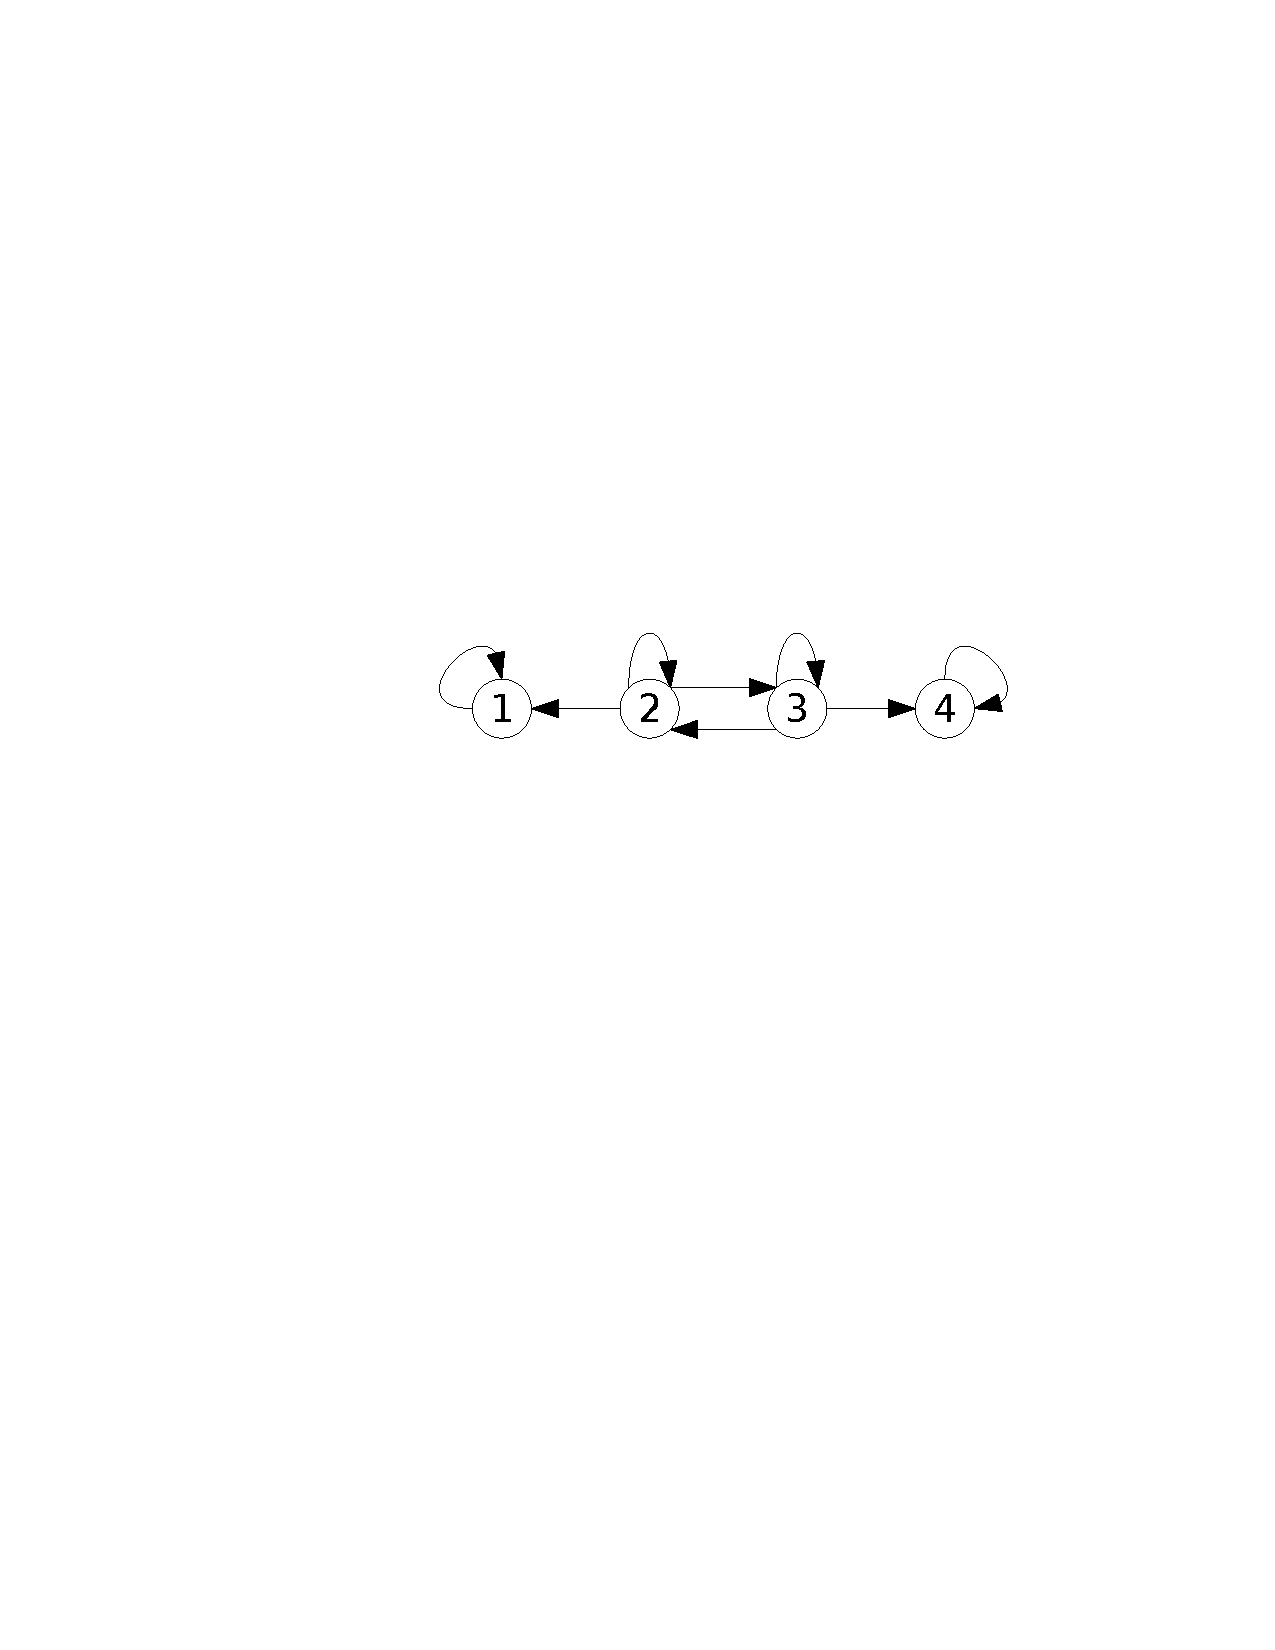
\includegraphics[width=0.45\textwidth]{../figs_08_genetics/graphe_absorbant}
\end{center}
\begin{enumerate}
\item Does the process eventually reach an absorbing state?
\item Average number of times spent in a transient state, if starting in a transient state?
\item Average number of steps before entering an absorbing state?
\item Probability of being absorbed by a given absorbing state, when there are more than one, when starting in a given transient state?
\end{enumerate}

Answer to question 1:
\begin{theorem}
In an absorbing Markov chain, the probability of reaching an absorbing state is 1.
\end{theorem}

For an absorbing chain with $k$ absorbing states and $r-k$ transient states, the transition matrix can be written in the following \textbf{standard form}:
\[
P=\begin{pmatrix}
\mathbb{I}_k & \mathbf{0} \\
R & Q
\end{pmatrix}
\]
with following meaning,
\begin{center}
\begin{tabular}{ccc}
& Absorbing states & Transient states \\
Absorbing states & $\mathbb{I}_k$ & $\mathbf{0}$ \\
Transient states & $R$ & $Q$
\end{tabular}
\end{center}
with $\mathbb{I}_k$ the $k\times k$ identity matrix, $\mathbf{0}$ an $k\times(r-k)$ matrix of zeros, $R$ an $(r-k)\times k$ matrix and $Q$ an $(r-k)\times(r-k)$ matrix.


The matrix $\mathbb{I}_{r-k}-Q$ is invertible. Let
\begin{itemize}
\item $N=(\mathbb{I}_{r-k}-Q)^{-1}$ be the \emph{fundamental matrix} of the Markov chain
\item $T_i$ be the sum of the entries on row $i$ of $N$
\item $B=NR$.
\end{itemize}
\vskip0.5cm
Answers to our remaining questions:
\begin{enumerate}
\setcounter{enumi}{1}
\item $N_{ij}$ is the average number of times the process is in the $j$th transient state if it starts in the $i$th transient state.
\item $T_i$ is the average number of steps before the process enters an absorbing state if it starts in the $i$th transient state.
\item $B_{ij}$ is the probability of eventually entering the $j$th absorbing state if the process starts in the $i$th transient state.
\end{enumerate}











\begin{definition}
A regular Markov chain is one in which $S^p$ is positive for some positive integer $p$.
\end{definition}

From Theorem \ref{Theo:NormRho}
$$\rho(S)\leq \| S\| _1 =1$$
then $|\lambda|\leq 1$ for all eigenvalues of a stochastic matrix. Furthermore, if $S$ is a stochastic matrix $\lambda =1$ is an eigenvalue of $S$; hence $\rho(S)=1$ and the dominant eigenvalue $\lambda _1 =1$. Then
$$\lim_{n\rightarrow +\infty}p(n)=\lim_{n\rightarrow +\infty}S^np(0)=cV_1$$
where $V_1=(v_1,v_2,\dots ,v_k)$ is the eigenvector that corresponds to the dominant eigenvalue $\lambda _1 =1$.

Since $p(n)=(p_1(n),p_2(n),\dots , p_k(n))^T$, we have $\sum_{i=1}^k p_i(n)=1$, it follows that
$$cv_1+cv_2+\dots cv_k=1.$$
Therefore
$$c=\frac{1}{v_1+v_2+\dots+v_k}.$$


\begin{definition}
A state $s_i$ in a Markov chain is said to be absorbing if whenever it occurs on the $n^{th}$ generation of the experiment, it then occurs on every subsequent repetition. In other word, if for some $p_{ii}=1$ then $p_{ij}=0$ for $i\not =j$.
\end{definition}

\begin{definition}
A Markov chain is said to be absorbing if it has at least one absorbing state, and if from every state it is possible to go to an absorbing state.
\end{definition}

In an absorbing Markov chain, a state that is not absorbing is called transient.

\chapter{Models using Markov chains}
\label{chap:genetics}

\section{A simple genetic model}
The simplest type of genetic inheritance of traits in animals occurs when a certain trait is determined by a specific pair of genes, each of which may be two types, say $G$ and $g$. An individual may have a $GG$ combination, a $Gg$ (genetically equivalent to $gG$), or $gg$ combination. An individual with $GG$ is said to be dominant, a $gg$ individual is recessive and a $Gg$ is an hybrid.

In the mating of two animals, the offspring inherits one gene of the pair from each parent: the basic assumption of genetics is that these genes are selected at
random, independently of each other.


This assumption determines the probability
of occurrence of each type of offspring: The offspring
\begin{itemize}
\item of two dominant parents must be dominant, 
\item of two recessive parents must be recessive,
\item and of one dominant and one recessive parent must be hybrid.
\end{itemize}
In the mating of a dominant and a hybrid animal, each offspring must get a
$G$ gene from the former and has an equal chance of getting $G$ or $g$ from the latter.
Hence there is an equal probability of getting a dominant or a hybrid offspring.
Again, in the mating of a recessive and a hybrid, there is an even chance for getting
either a recessive or a hybrid. In the mating of two hybrids, the offspring has an
equal chance of getting $G$ or $g$ from each parent. Hence the probabilities are $1/4$
for $GG$, $1/2$ for $Gg$, and $1/4$ for $gg$.

A certain trait is determined by a specific pair of genes, each of which may be two types, say $G$ and $g$. 
One individual may have:
\begin{itemize}
\item $GG$ combination (\emph{dominant})
\item $Gg$ or $gG$, considered equivalent genetically (\emph{hybrid})
\item $gg$ combination (\emph{recessive})
\end{itemize}
In sexual reproduction, offspring inherit one gene of the pair from each parent. 


\subsection{Basic assumption of Mendelian genetics}
Genes inherited from each parent are selected at random, independently of each other.
This determines probability
of occurrence of each type of offspring. The offspring
\begin{itemize}
\item of two $GG$ parents must be $GG$, 
\item of two $gg$ parents must be $gg$,
\item of one $GG$ and one $gg$ parent must be $Gg$,
\item other cases must be examined in more detail.
\end{itemize}


\paragraph{$GG$ and $Gg$ parents}
\begin{center}
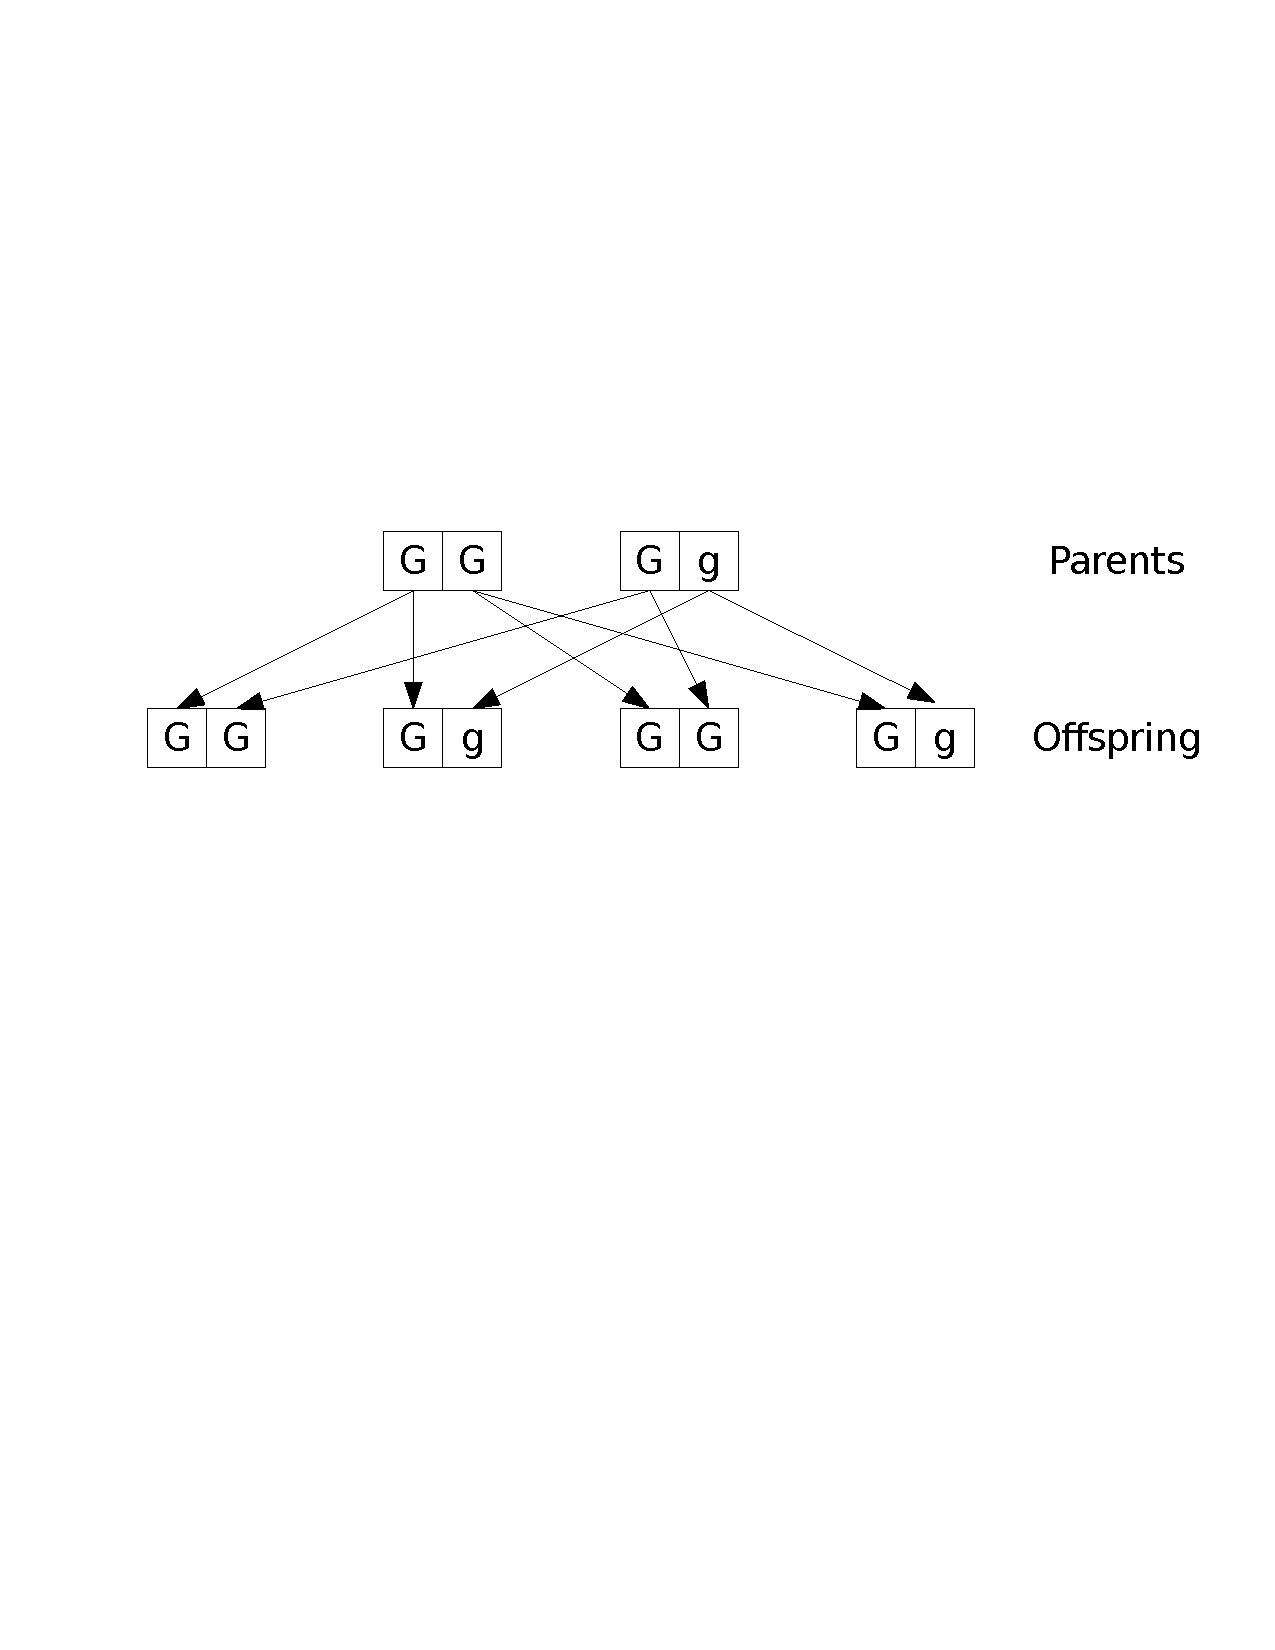
\includegraphics[width=0.5\textwidth]
{../figs_08_genetics/dominant_hybrid}
\end{center}
\vskip0.2cm
Offspring has probability $\dfrac 12$ of being $GG$ and $\dfrac 12$ of being $Gg$.

\paragraph{$Gg$ and $Gg$ parents}
\begin{center}
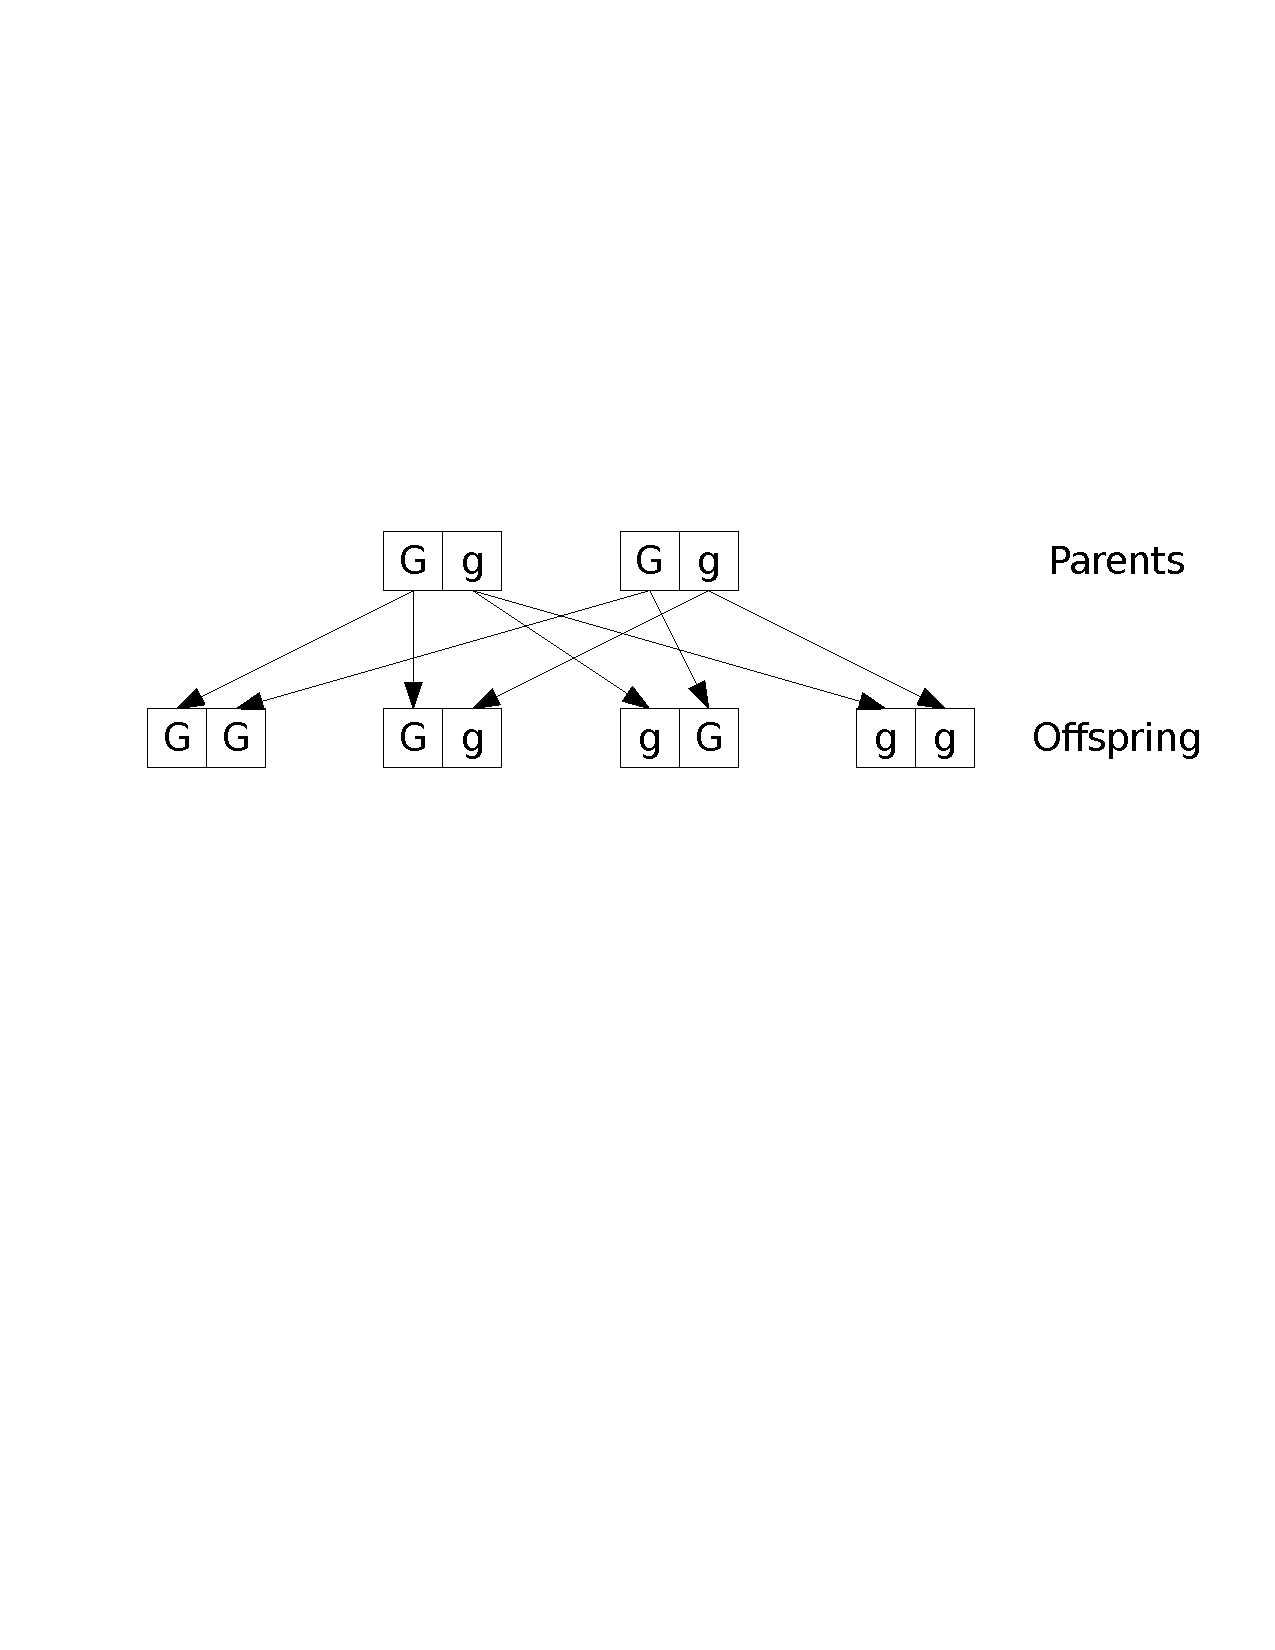
\includegraphics[width=0.5\textwidth]
{../figs_08_genetics/hybrid_hybrid}
\end{center}
\vskip0.2cm
Offspring has probability $\dfrac 14$ of being $GG$, $\dfrac 12$ of being $Gg$ and $\dfrac 14$ of being $gg$.


\paragraph{$gg$ and $Gg$ parents}
\begin{center}
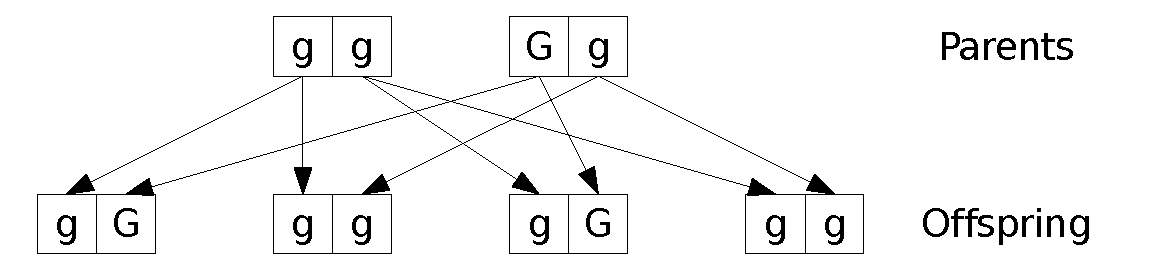
\includegraphics[width=0.5\textwidth]
{../figs_08_genetics/recessive_hybrid}
\end{center}
\vskip0.2cm
Offspring has probability $\dfrac 12$ of being $Gg$ and $\dfrac 12$ of being $gg$.


\subsection{A first genetic model -- Regular Markov chain}
Consider a process of continued matings with the following characteristics:
\begin{itemize}
\item Start with an individual of known or unknown
genetic character and mate it with a hybrid. 
\item Assume that there is at least one
offspring; choose one of them at random and mate it with a hybrid.
\item Repeat this process through a number of generations. 
\end{itemize}
The genetic type of the chosen
offspring in successive generations can be represented by a Markov chain, with states $GG$, $Gg$ and $gg$. So there are 3 possibles states $S_1=GG$, $S_2=Gg$ and $S_3=gg$.
We have
\begin{center}
\begin{tabular}{c|ccc}
$\nearrow$ & GG & Gg & gg \\
\hline
GG & 0.5 & 0.5 & 0 \\
Gg & 0.25 & 0.5 & 0.25 \\
gg & 0 & 0.5 & 0.5
\end{tabular}
\end{center}
The transition probabilities are thus
\[
P=\left (
\begin{array}{ccc}
\frac 12 & \frac 12 & 0 \\
\frac 14 & \frac 12 & \frac 14 \\
0 & \frac 12 & \frac 12
\end{array}\right).
\]
The (di)graph associated to $P$ is shown in Figure~\ref{fig:Markov_graph1}.
\begin{figure}[htbp]
\begin{center}
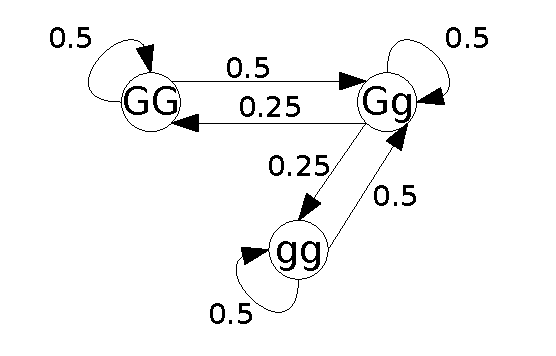
\includegraphics[width=0.5\textwidth]{../figs_08_genetics/graphe_hybride}
\caption{Transition graph for the Markov chain for the genetics model with mating with an hybrid individual.}
\label{fig:Markov_graph1}
\end{center}
\end{figure}
The Markov chain with transition matrix $P$ is regular. Indeed, compute $P^2$:
\[
P^2=\left (
\begin{array}{ccc}
\frac 38 & \frac 12 & \frac 18 \\
\frac 14 & \frac 12 & \frac 14 \\
\frac 18 & \frac 12 & \frac 38
\end{array}\right)
\]
As all entries are positive, $P$ is primitive and the Markov chain is regular. It is also possible to check this information directly by looking at the graph associated to the Markov chain (Figure~\ref{fig:Markov_graph1}). There, it is easy to check that it is possible to go from any state to any other state, i.e., the graph is strongly connected. From Theorem~\ref{th:connected_equiv_irreducible}, it follows that the matrix $P$ is irreducible. Further, the self-connecting loops mean that Theorem~\ref{} can be used, implying the primitivity of $P$.

Compute the left eigenvector associated to 1 by solving
\[
(w_1,w_2,w_3)
\left (
\begin{array}{ccc}
\frac 12 & \frac 12 & 0 \\
\frac 14 & \frac 12 & \frac 14 \\
0 & \frac 12 & \frac 12
\end{array}\right)=(w_1,w_2,w_3)
\]
\begin{subequations}
\begin{align}
\frac 12 w_1+\frac 14 w_2 &= w_1 \label{eq:l1} \\
\frac 12 w_1+\frac 12 w_2+\frac 12 w_3 &= w_2 \label{eq:l2} \\
\frac 14 w_2+\frac 12 w_3 &= w_3 \label{eq:l3} 
\end{align}
\end{subequations}
From \eqref{eq:l1}, $w_1=w_2/2$, and from \eqref{eq:l3}, $w_3=w_2/2$. Substituting these values into \eqref{eq:l2},
\[
\frac 14 w_2+\frac 12 w_2 +\frac 14 w_2=w_2,
\]
that is, $w_2=w_2$, i.e., $w_2$ can take any value. So $w=(\frac 14,\frac 12,\frac 14)$.



\subsection{A second genetic model -- Absorbing Markov chain}
Suppose now that we conduct the same experiment, but mate the individual picked at random in each new generation with a $GG$ individual instead of a $Gg$ individual. The transition table is
\begin{center}
\begin{tabular}{c|ccc}
$\nearrow$ & GG & Gg & gg \\
\hline
GG & 1 & 0 & 0 \\
Gg & 0.5 & 0.5 & 0 \\
gg & 0 & 1 & 0
\end{tabular}
\end{center}
and the resulting transition probabilities are
\[
P=\left (
\begin{array}{ccc}
1 & 0 & 0 \\
\frac 12 & \frac 12 & 0 \\
0 & 1 & 0
\end{array}\right)
\]

\begin{figure}[htbp]
\begin{center}
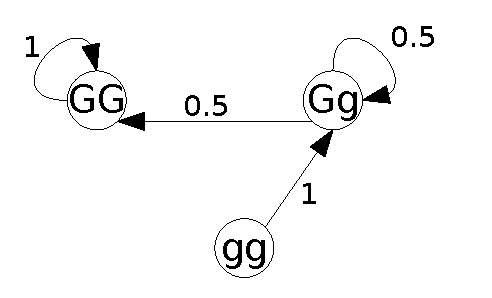
\includegraphics[width=0.45\textwidth]{../figs_08_genetics/graphe_dominant}
\caption{Transition digraph for the Markov chain for the genetics model with mating with a dominant individual. This graph is not strongly connected; vertex $GG$ is a \emph{sink}, while vertex $gg$ is a \emph{source}, or, in Markov chain vocabulary, state $GG$ is absorbing and state $gg$ is repulsive.}
\label{fig:Markov_graph2}
\end{center}
\end{figure}


Clearly,
\begin{itemize}
\item the process leaves $gg$ after one iteration, and can never return,
\item as soon as the process leaves $Gg$, it can never return there,
\item and it can never leave $GG$ as soon as it gets there.
\end{itemize}

The matrix is already in standard form,
\[
P=\left (
\begin{array}{ccc}
1 & 0 & 0 \\
\frac 12 & \frac 12 & 0 \\
0 & 1 & 0
\end{array}\right)
=\begin{pmatrix}
\mathbb{I}_1 & \mathbf{0} \\
R & Q
\end{pmatrix},
\]
with $\mathbb{I}_1=1$, $\mathbf{0}=(0\;\; 0)$ and
\[
R=\begin{pmatrix}
\frac 12\\ 0
\end{pmatrix}
\qquad
Q=\begin{pmatrix}
\frac 12 & 0\\
1 & 0
\end{pmatrix}.
\]
We have
\[
\mathbb{I}_2-Q=\begin{pmatrix}
1 & 0 \\
0 & 1
\end{pmatrix}
-\begin{pmatrix}
\frac 12 & 0\\
1 & 0
\end{pmatrix}
=\begin{pmatrix}
\frac 12 & 0\\
-1 & 1
\end{pmatrix},
\]
so
\[
N=(\mathbb{I}_2-Q)^{-1}=
2\begin{pmatrix}
1 & 0 \\
1 & \frac 12
\end{pmatrix}=
\begin{pmatrix}
2 & 0 \\
2 & 1
\end{pmatrix}.
\]
Then
\[
T=N\nbOne=\begin{pmatrix}
2\\
3
\end{pmatrix}
\]
and
\[
B=NR=
\begin{pmatrix}
2 & 0 \\
2 & 1
\end{pmatrix}
\begin{pmatrix}
\frac 12\\ 0
\end{pmatrix}
=
\begin{pmatrix}
1\\ 1
\end{pmatrix}.
\]

\part{Ordinary differential equations}
\chapter{A brief theory of ordinary differential equations}
\label{chap:theory_ode}


In this chapter, we consider ordinary differential equations of first-order,
\begin{equation}\label{eq:1st_order_ODE_nonauton}
x'=f(t,x),
\end{equation}
with $x\in\IR^n$ and $f:\IR\times\IR^n\to\IR^n$, as well as $p$th-order ordinary differential equations of the form
\begin{equation}\label{eq:pth_order_ODE}
x^{(p)}=f(t,x,x',\ldots,x^{(p-1)}),
\end{equation}
where $x\in\IR$ and $x^{(k)}$ denotes the $k$th derivative of $x(t)$. These two equations are said to be in \emph{normal form}, and form a subset of a larger class of first-order and $p$th-order differential equations, defined respectively by $F(t,x,x')=0$ and $F(t,x,x',\ldots,x^{(p)})=0$. We could also consider vector-valued $p$th-order equations.
However, \eqref{eq:1st_order_ODE} and \eqref{eq:pth_order_ODE} are sufficient for our purpose, and we limit our attention to them.

\section{First definitions}
A system such as \eqref{eq:1st_order_ODE} is \emph{nonautonomous}, since the function $f$ depends explicitly on $t$ (time). Much of the theory in this chapter will concern specifically the \emph{autonomous} system,
\begin{equation}\label{eq:1st_order_ODE}
x'=f(x),
\end{equation}
where $x\in\IR^n$ and $f:\IR^n\to\IR^n$.

\begin{definition}
An equilibrium solution of equation \eqref{eq:1st_order_ODE} is a solution $\bar x$ satisfying 
\[
f(\bar x)=0.
\]
\end{definition}
The system at $x=\bar x$ is then said to be at equilibrium. Indeed, since $f(\bar x)=0$, we have
\[
\frac{d}{dt}\bar x(t)=f(\bar x(t))=0,
\]
and thus the system is ``at rest''. Equilibria are then classified in terms of their \emph{stability}. We return to this concept later, but we give the definitions now because they appear throughout this chapter.
\begin{definition}(Local stability)
An equilibrium solution $\bar x$ of \eqref{eq:1st_order_ODE} is \emph{locally stable} if for each $\epsilon>0$ there exits a $\delta >0$ such that every solution $x(t)$ of \eqref{eq:1st_order_ODE} with the initial condition $x(t_0)=x_0$,
$$\| x_0-\bar x\|_2< \delta,$$
satisfies the condition that
$$\| x(t)-\bar x\|_2< \epsilon$$
for all $t \geq t_0$.
If the equilibrium solution is not locally stable it is said to be \emph{unstable}.
\end{definition}

Euclidian distance between two points $Y_1=(y_1^1,y_2^1,\dots,y_n^1)$ and $Y_2=(y_1^2,y_2^2,\dots,y_n^2)$ in $\mathbb{R}^n$ is $$\|Y_1-Y_2\|_2=\sqrt{\sum _{i=1}^n(y_i^1-y_i^2)^2}.$$

\begin{definition}(Local asymptotic stability) 
An equilibrium solution $\bar x$ of \eqref{eq:1st_order_ODE} is \emph{locally asymptotically stable} if it is locally stable and if there exist $\gamma >0$ such that $\| x_0-\bar x\| _2< \gamma$ implies
$$\lim_{t\rightarrow \infty}\| x(t)-\bar x\| _2=0.$$
\end{definition}


\begin{definition}(Periodic solution)
A \emph{periodic solution} of the system \eqref{eq:1st_order_ODE} is a nonconstant solution $x(t)$ satisfying $x(t+T)=x(t)$ for all $t$ on the interval of existence  for some $T>0$. The minimum value of $T$ is called the period of the solution.
\end{definition}

\section{First-order differential equations}
\begin{definition}
The standard form of first order linear
equations is
$$\frac{dy}{dt}+p(t)y=g(t)$$
$p$ and $g$ are given functions of the independent variable $t$.
\end{definition}


\subsection{Analytical methods}


{\bf Linear equations: Integrating factors}



To solve $1^{st}$ order linear equation with non-constant coefficients (this method can also be used for equation with constant coefficient).
\begin{enumerate}
\item Put the DE in the standard form
\begin{equation}\frac{dy}{dt}+p(t)y=g(t)\label{eq:DE}\end{equation}
\item Determine the integrating factor $\mu (t)$
\begin{itemize}
\item Multiply the DE (\ref{eq:DE}) by $\mu (t)$
\begin{equation}\mu (t)\frac{dy}{dt}+\mu (t)p(t)y=\mu
(t)g(t)\label{eq:DE1}\end{equation} 
\item  State that the left side of (\ref{eq:DE1}) is equal to $\frac{d}{dt}(\mu (t)y)$
$$\frac{d}{dt}(\mu (t)y)=\mu (t)\frac{dy}{dt}+y\frac{d \mu}{dt}=\mu (t)\frac{dy}{dt}+\mu
(t)p(t)y$$
\item Solve for $\mu (t)$
$$\frac{d \mu }{dt}=\mu (t) p(t)$$
\end{itemize}
$$\Rightarrow \quad \mu(t)=e^{\int p(t)dt}$$
\item Solve (\ref{eq:DE1}) for $y$ with $\mu(t)=e^{\int p(t)dt}$
$$\left(\frac{d}{dt}e^{\int p(t)dt}y=\right)e^{\int p(t)dt}\frac{dy}{dt}+p(t)e^{\int p(t)dt}y=e^{\int p(t)dt}g(t)$$
$$\frac{d}{dt}\mu(t)y=\mu(t)g(t)$$
$$\mu(t)y=\int \mu(t)g(t)dt +c$$
\end{enumerate}

Hence the general solution of (\ref{eq:DE}) is
$$y(t)=\frac{1}{\mu(t)}\left [\int_{t_0}^t \mu(s)g(s)ds +c\right ]
\quad with \quad \mu(t)=e^{\int p(t)dt}$$




{\bf Separable equations}



\begin{definition}(Separable equations) A first order differential equation
$$\frac{dy}{dx}=f(x,y)$$
is said to be separable or to have separable variables if it can be
expressed as follows
$$\frac{dy}{dx}=g(x)h(y)$$
(the rate function can be expressed as a product of a function of
the independent variable times a function of the dependent variable
).
\end{definition}


{\bf To solve separable equations: }
$\frac{dy}{dx}=g(x)h(y)$
\begin{enumerate}
\item Express the separable equation as follows
$$\frac{1}{h(y)}\frac{dy}{dx}=g(x)$$
\item As $y$, $\frac{dy}{dx}$, and $g(x)$ are functions of $x$,
apply the integral
$$\int \frac{1}{h(y)}\frac{dy}{dx} dx=\int g(x) dx$$
\item Use the Change of variable Theorem (if $u=v(x)$ $\int f(v(x))v'(x)dx=\int
f(u)du$) for the left side with $u=y(x)$
$$\int \frac{1}{h(u)}du=\int g(x) dx$$
$$\int \frac{1}{h(y)}dy=\int g(x) dx$$
\item Integrate
\begin{equation}H(y)=G(x)+c\label{eq:GS}\end{equation} $c$ is the combination of the left
and right integration constants, $H$ and $G$ are antiderivatives of
$\frac{1}{h(y)}$ and $g(x)$ respectively. \item Solve equation
(\ref{eq:GS}) for $y$ to obtain a explicit form of the general
solution.
\end{enumerate}



\subsubsection{Local stability}
A simple criterion for determining the L.A.S. of an equilibrium solution to a first order autonomous differential equation
\begin{equation}
\label{eq:ODE1Nonlin}
\frac{dy}{dt}=f(y)
\end{equation}
having an equilibrium at $\bar y$.


\begin{theorem}
Suppose $f'$ is continuous on an open interval $I$ containing $\bar y$, where $\bar y$ is an equilibrium of $\frac{dy}{dt}=f(y)$. Then $\bar y$ is locally asymptotically stable if $$f'(\bar y)<0$$
and unstable if $f'(\bar y)>0$.
\end{theorem}

The value $f'(\bar y)$ is know as the eigenvalue of the linearized equation.


\begin{definition}
The equilibrium $\bar y$ of $\frac{dy}{dt}=f(y)$ is called hyperbolic if $f'(\bar y)\not =0$. Otherwise, it is called nonhyperbolic.
\end{definition}


Nonhyperbolic equilibria have a zero eigenvalue, and hence their local stability is indeterminate.


\subsubsection{Phase line analysis}
Consider a first-order nonautonomous equation
$$\frac{dy}{dt}=f(t,y).$$
$f(t,y)$ represents the slope of the tangent to the solution $y(t)$ at the point $(t,y)$. Hence $f(t,y)$ can be used to construct a direction field in the $t,y-$plane.

Consider a first-order autonomous equation
$$\frac{dy}{dt}=f(y).$$
Here the direction of flow does not change with $t$. Hence it is only necessary to determine the direction of flow on the $y-$axis (Phase line). If $\frac{dy}{dt}$ is positive, the direction of flow is in the positive direction, if it is negative, the flow is in negative direction.



\subsection{Higher-order linear equations}
The general solution to an $n^{th}-$order linear nonhomogeneous differential equation is the sum of two solutions, a general solution to the homogeneous differential equation and a particular solution to the nonhomogeneous differential equation
$$y(t)=y_h(t)+y_p(t).$$ 



{\bf $\bullet$} Methodology to find the general solution to the homogeneous equation is given for second-order linear equations, but it can be generalized to the $n^{th}-$order linear equations.


\begin{theorem} (Principle of superposition)
If $y_1$ and $y_2$ are two solutions of the homogeneous linear differential
equation on an interval $I$


$$y''+p(t)y'+q(t)y=0$$

then the linear combination $$c_1y_1+c_2y_2$$ is also a solution for
any values of the constants $c_1$ and $c_2$ on the interval.
\end{theorem}

\begin{definition}(Wronskian)
Suppose each of the functions $f_1(t),
f_2(t), \dots, f_n(t)$ has at least $n-1$ derivatives. The
determinant

$$W(f_1,f_2,\dots,f_n)=\left |
\begin{array}{llll}
f_1 & f_2 & \cdots & f_n\\
f_1' & f_2' & \cdots & f_n'\\
\vdots & \vdots & &\vdots\\
f_1^{(n-1)} & f_2^{(n-1)} & \cdots & f_n^{(n-1)}\\
\end{array}
\right |$$ is called the Wronskian of the functions.
\end{definition}


\begin{theorem}
Let $y_1$ and $y_2$ be solutions of the differential equation
$$
y''+p(t)y'+q(t)y=0$$ where $p$ and $q$ are continuous on an open
interval $I$. Then $y_1$ and $y_2$ are linearly independent on $I$
if and only if $W(y_1,y_2)(t)\not=0$ $\forall t \in I$.
\end{theorem}

\begin{definition}
Any set $y_1$, $y_2$ of 2 linearly independent solutions of
$$
y''+p(t)y'+q(t)y=0$$ on an open interval $I$ is said to be {\bf a
fundamental set of solutions} on $I$ of the differential equation.
\end{definition} 


\begin{definition}
The general solution of
$$y''+p(t)y'+q(t)y=0$$ on an open interval $I$ is the linear combination of 2 linearly independent solutions $y_1$ and $y_2$
$$y(t)=c_1 y_1(t)+c_2y_2(t)$$
with $c_1$ and $c_2$ constants. $y_1$ and $y_2$ form a fundamental set of solutions.
\end{definition}


{\bf Method for linear homogeneous
second-order equations with constant coefficients}
\begin{equation}
ay''+by'+cy=0\label{eq:constant}
\end{equation}
Let assume that the solution can take the form of $$y(t)=e^{rt}.$$
\vspace{-.2cm}
 \begin{enumerate}
\item Write the {\bf characteristic equation }
$$ar^2+br+c=0$$
\item Find the {\bf roots} $r_1$ and $r_2$ of the characteristic equation
$$r_1=\frac{-b-\sqrt{\Delta}}{2a} , \qquad r_2=\frac{-b+\sqrt{\Delta}}{2a}, \quad \textrm{with} \quad \Delta=b^2-4ac $$
\begin{description}
\item[$\Delta >0$]: $r_1$, $r_2$ distinct and real,
$y_1(t)=e^{r_1t}$ and $y_2(t)=e^{r_2t}$ are 2 linearly independent
solutions of \eqref{eq:constant}. The general solution is
$$y(t)=c_1 e^{r_1t}+c_2e^{r_2t}, \quad c_1, c_2\textrm{ arbitrary constants}$$
\item[$\Delta =0$]: $r_1=r_2=r$ real, $y_1(t)=e^{rt}$ and $y_2(t)=te^{rt}$ are 2 linearly independent
solutions of \eqref{eq:constant}. The general solution is
$$y(t)=c_1 e^{rt}+c_2te^{rt} , \quad c_1, c_2\textrm{ arbitrary constants}$$
\item[$\Delta <0$]: $r_1$, $r_2$ complex conjugates, $r_1=\alpha + i \mu$ and $r_2=\alpha - i
\mu$. $y_1(t)=e^{\alpha t}\cos (\mu t)$ and $y_2(t)=e^{\alpha t}\sin
(\mu t)$ are 2 linearly independent solutions of
\eqref{eq:constant}. The general solution is
$$y(t)=c_1 e^{\alpha t}\cos (\mu t)+c_2e^{\alpha t}\sin (\mu t) , \quad c_1, c_2\textrm{ arbitrary constants}$$
\end{description}
\end{enumerate}

Note that an $n^{th}-$order linear homogeneous differential equation always has a solution equal to zero $y(t)\equiv 0$. When the equation has constant coefficients, the stability of the zero solution is stable (when a solution to an IVP will tend to zero). Stability of the zero solution depends on the eigenvalues, the roots of $\lambda_i$ of the characteristic equation.

\begin{theorem}
If all of the roots of the characteristic polynomial $P(\lambda)$ are negative or have negative real part, then given any solution $y(t)$ of the homogeneous differential equation $$\frac{d^n y}{dy^n}+a_1(t)\frac{d^{n-1}y}{dy^{n-1}}+\dots+a_{n-1}(t)\frac{dy}{dy}+a_n(t)y=0,$$ there exist positive constant $M$ and $b$ such that
$$|y(t)|\leq Me^{-bt}\quad for \quad t>0$$
and
$$\lim _{t\rightarrow \infty} |x(t)|=0$$
\end{theorem}




Methodologies to find a particular solution to the nonhonogeneous differential equation:
\begin{itemize}
\item Undetermined coefficients
\item Variation of parameters
\end{itemize}


{\bf Undetermined coefficients (to find
a particular solution $Y(t)$)}
\begin{itemize}
\item Make an assumption about the form of the particular solution
$Y(t)$ but with the coefficients unspecified
\item The particular solution has to satisfy the nonhomogeneous
equation $\Leftrightarrow$ Substitute the assumed expression of
$Y(t)$ in the nonhomogeneous equation $\Rightarrow$ Coefficients to
be determined
\end{itemize}
Conditions for application: 
if $g(t)$ takes the form: constant function, exponential, polynomial, sine, cosine, any sum or products of such functions.
$$y''+p(t)y'+q(t)y=g(t)$$
\begin{itemize}
\item Make an assumption about the form of the particular solution
 $Y(t)$: if $g(t)$ is of the form in the left column or is the sum or product of such function, then check a particular solution $Y(t)$ of the corresponding form as indicated in the right column
\begin{center}
\begin{tabular}{l|l}
$\mathbf{g(t)}$ & {\bf Assumed form of }$Y(t)$\\
$\alpha e^{\beta t}$& $ae^{\beta t}$\\
$\alpha \cos (\omega t) +\beta \sin (\omega t)$ & $a \cos (\omega t)
+b \sin (\omega t)$\\
$\alpha$ & $a$\\
$\alpha + \beta t$ & $a +bt$\\
$\alpha + \beta t +\gamma t^2$ & $a +bt +ct^2$\\
$\alpha + \beta t +\gamma t^2+ \cdots+\delta t^m$ & $a +bt +ct^2+ \cdots+d t^m$\\
\end{tabular}
\end{center}
\item If coefficients cannot be determined, then no solution of this
form exists $\Rightarrow$ modify the assumption
\item If $g(t)$ contains terms that duplicate any solutions of the corresponding homogeneous equation
$\Rightarrow$ each such term must be multiplied by $t^s$
($s$ the smallest natural number that eliminates the
duplication).
\end{itemize}


{\bf Variation of parameters: }
$y''+p(t)y'+q(t)y=g(t)$
\begin{enumerate}
\item Find the {\bf general solution of the homogeneous
equation} $\Leftrightarrow$ Find 2 linearly independent solutions
$y_1$ and $y_2$ of the homogeneous equation
\item Check for the nonhomogeneous equation a solution of the form
$$Y(t)=u_1(t)y_1(t)+u_2(t)y_2(t)$$
where $u_1$ and $u_2$ are two functions of $t$ to be determined, and
that satisfy the {\bf second condition}
$$u_1'(t)y_1(t)+u_2'(t)y_2(t)=0$$
\item Substitute $Y(t)$ in the nonhomogeneous equation and use the
second condition to obtain
$$u'_1(t)y_1'(t)+u_2'(t)y_2'(t)=g(t)$$
\item Solve  the system of 2 linear algebraic
equation for $u_1'$ and $u_2'$
$$\left \{
\begin{array}{ll}
u_1'(t)y_1(t)+u_2'(t)y_2(t)&=0\\
u'_1(t)y_1'(t)+u_2'(t)y_2'(t)&=g(t)
\end{array}\right . \mathrm{or} \quad
\left [
\begin{array}{ll}
y_1(t)&y_2(t)\\
y_1'(t)&y_2'(t)
\end{array}\right ]\left [
\begin{array}{l}
u_1'(t)\\
u_2'(t)
\end{array}\right ]=\left [
\begin{array}{l}
0\\
g(t)
\end{array}\right ]
$$

$$\Rightarrow u_1'(t)=\frac{-y_2(t)g(t)}{W(y_1,y_2)(t)}, \qquad u_2'(t)=\frac{y_1(t)g(t)}{W(y_1,y_2)(t)}$$
\item Integrate, evaluate the integral omitting the integration
constants
$$\Rightarrow u_1(t)=-\int \frac{y_2(t)g(t)}{W(y_1,y_2)(t)}dt, \qquad u_2(t)=\int \frac{y_1(t)g(t)}{W(y_1,y_2)(t)}dt$$
\item A {\bf particular solution} of the nonhomogeneous equation is
$$Y(t)=-y_1(t)\int \frac{y_2(t)g(t)}{W(y_1,y_2)(t)}dt + y_2(t)\int \frac{y_1(t)g(t)}{W(y_1,y_2)(t)}dt$$
\item The {\bf general solution} of the nonhomogeneous equation is
$$y(t)=c_1y_1(t)+c_2y_2(t)+Y(t), \qquad c_1, \; c_2 \; \textrm{arbitrary constants}$$
\end{enumerate}


\begin{theorem}
If the functions $p$, $q$ and $g$ are continuous on an open interval
$I$, and if the functions $y_1$ and $y_2$ are linearly independent
solutions of the homogeneous equation, $y''+p(t)y'+q(t)y=0$,
corresponding to the nonhomogeneous equation
$$y''+p(t)y'+q(t)y=g(t)$$
then a particular solution of the nonhomogeneous equation is
$$Y(t)=-y_1(t)\int_{t_0}^t \frac{y_2(s)g(s)}{W(y_1,y_2)(s)}ds+y_2(t)\int_{t_0}^t \frac{y_1(s)g(s)}{W(y_1,y_2)(s)}ds$$
where $t_0$ is any point in $I$. The general solution is
$$y(t)=c_1y_1(t)+c_2y_2(t)+Y(t).$$
\end{theorem}

\section{Systems of linear equations}
A $n-$dimensional linear system
$$\frac{dX}{dt}=A X$$
where $A$ is a $n\times n$ constant matrix with real elements. The general solution of this system is
$$X(t)=e^{At}C$$
where $e^{At}$ is a $n\times n$ matrix known as the fundamental matrix and $C$ ia a $n\times 1$ vector. There exist many methods to compute the matrix exponential. To compute the general solution of the $n-$dimensional system, a straightforward method can be used (similar method used for higher-order constant coefficient DE).




Here the case of a 2-dimensional linear system is studied. 
Consider a system of first-order linear equations
\begin{equation}
\frac{dX}{dt}=A X
\label{eq:SysLin}
\end{equation}
where $X=(x_1,x_2)^T$ and $A$ is a constant $2\times 2$ matrix. Note that the zero solution $X=0$ is solution of the differential equation. 

Let $X=e^{\lambda t}V$ be a solution of \eqref{eq:SysLin}, then
$$AV=\lambda V$$
where $\lambda $ is the eigenvalue of $A$ and $V$ is the eigenvector corresponding to $\lambda$. The eigenvalues are solutions of $$\det (A-\lambda I)=0.$$
Then
$$\lambda ^2 -\tr (A) \lambda + \det (A)=0.$$
Solutions of \eqref{eq:SysLin} can take 3 different forms
\begin{itemize}
\item if eigenvalues are real and distinct
$$X(t)=c_1V_1 e^{\lambda _1t}+c_2V_2 e^{\lambda _2t}$$
with $c_1$ and $c_2$ constant.
\item if eigenvalues are real and equal
$$X(t)=c_1V_1 e^{\lambda _1t}+c_2\left (V_1te^{\lambda _1t}+P e^{\lambda _1t}\right )$$
with $c_1$ and $c_2$ constant. $P$ can be obtained by solving $(A-\lambda _1 I)P=V_1$.
\item if eigenvalues are complex conjugate $\lambda _{1,2}=a\pm i b$
$$X(t)=P_1 e^{at} \cos (bt) + P_2 e^{at}\sin (bt).$$
\end{itemize}
Behaviors of solutions:
\begin{itemize}
\item The origin is asymptotically stable if the eigenvalues of $A$ are negative or have negative real part.
\item The origin is stable if the eigenvalues of $A$ are nonpositive or have nonpositive real part.
\item The origin is unstable if the eigenvalues of $A$ are positive or have positive real part.
\end{itemize}


\begin{theorem}
Suppose $\frac{dX}{dt}=A X$ where $A$ is a constant $2\times 2$ matrix with $\det (A) \not =0$. 

The orign is asymptotically stable iff
$$\tr(A)<0 \quad and \quad \det (A)>0.$$

The orign is stable iff
$$\tr(A)\leq 0 \quad and \quad \det (A)>0.$$


The origin is unstable iff 
$$\tr(A)> 0 \quad or \quad \det (A)<0.$$
\end{theorem}


In the case of real eigenvalues $\lambda _1$ and $\lambda _2$, the eigenvectors $V_1$ and $V_2$ are directions along which solutions travel toward or away the origin:
\begin{itemize}
\item if $\lambda _1$ is positive, solutions will travel along $V_1$ away from the origin.
\item if $\lambda _2$ is negative, solutions will travel along $V_2$ toward the origin.
\end{itemize}
Hence solutions travel in a direction which corresponds to a linear combination of $V_1$ and $V_2$
\begin{theorem}
Consider a system of first order linear equations
$$\frac{dX}{dt}=A X$$
where $X=(x_1,x_2)^T$ and $A$ is a $2\times 2-$matrix.
\begin{itemize}
\item if $\det A >0$ and $\tr A ^2 -4 \det A\geq 0$ then the origin is a node (real eigenvalues having the same signs); a stable node if $\tr A <0$ (real $\lambda _{1,2}<0$), and an unstable node if $\tr A >0$ (real $\lambda _{1,2}>0$).
\item if $\det A <0$ then the origin is a saddle (real eigenvalues have opposite signs, $\lambda _1 \lambda _2<0$).
\item if $\det A >0$ and $\tr A ^2 -4 \det A < 0$ and $\tr A \not =0$, the origin is a spiral (complex conjugate with nonzero real part); it is stable if $\tr A <0$ (negative real part) and unstable if $\tr A >0$ (positive real part).
\item if $\det A >0$ and $\tr A=0$ then the origin is a center (purely imaginary eigenvalues $\lambda _{1,2}=\pm ib$).
\end{itemize}
\end{theorem}



\section{Linear systems of ODE}
\begin{definition}[Linear ODE]
A \emph{linear} ODE is a differential equation taking the form
\begin{equation}\label{sys:linear_general}
\frac{d}{dt}x=A(t)x+B(t),
\end{equation}
where $A(t)\in\mathcal{M}_n(\IR)$ with continuous entries, $B(t)\in\IR^n$ with real valued, continuous coefficients, and $x\in\IR^n$. The associated IVP takes the form 
\begin{equation}\label{sys:IVP_linear_general}
\begin{aligned}
\frac{d}{dt}x &= A(t)x+B(t) \\
x(t_0)&=x_0.
\end{aligned}
\end{equation}
\end{definition}

\paragraph{Types of systems:}
\begin{itemize}
\item $x'=A(t)x+B(t)$ is linear nonautonomous ($A(t)$ depends on $t$) nonhomogeneous (also called \emph{affine} system).
\item $x'=A(t)x$ is linear nonautonomous homogeneous.
\item $x'=Ax+B$, that is, $A(t)\equiv A$ and $B(t)\equiv B$, is linear autonomous nonhomogeneous (or affine autonomous).
\item $x'=Ax$ is linear autonomous homogeneous.
\end{itemize}
\begin{itemize}
\item If $A(t+T)=A(t)$ for some $T>0$ and all $t$, then linear periodic.
\end{itemize}



\begin{theorem}[Existence and Uniqueness]
Solutions to \eqref{sys:IVP_linear_general} exist and are unique on the whole interval over which $A$ and $B$ are continuous.
In particular, if $A,B$ are constant, then solutions exist on $\IR$.
\end{theorem}


\frame{\frametitle{Autonomous linear systems}
Consider the autonomous affine system
\begin{equation}\label{sys:affine_auton}
\frac{d}{dt}x=Ax+B,
\end{equation}
and the associated homogeneous autonomous system
\begin{equation}\label{sys:lin_auton}
\frac{d}{dt}x=Ax.
\end{equation}
}

\subsection{Exponential of a matrix}
\begin{definition}[Matrix exponential]
Let $A\in\M_n(\IK)$ with $\IK=\IR$ or $\IC$. The \emph{exponential} of $A$, denoted $e^{At}$, is a matrix in $\M_n(\IK)$, defined by
\[
e^{At}=\II +\sum_{k=1}^\infty \frac{t^k}{k!}A^k,
\]
where $\II$ is the identity matrix in $\M_n(\IK)$.
\end{definition}

\paragraph{Properties of the matrix exponential}
\begin{itemize}
\item $e^{At_1}e^{At_2}=e^{A(t_1+t_2)}$ for all $t_1,t_2\in\IR$.
\item $Ae^{At}=e^{At}A$ for all $t\in\IR$. [$A$ and $e^{At}$ commute]
\item $(e^{At})^{-1}=e^{-At}$ for all $t\in\IR$.
\end{itemize}
\begin{theorem}\label{th:solution_matrix_exponential}
The unique solution $\phi$ of \eqref{sys:lin_auton} with initial condition $\phi(t_0)=x_0$ is given by
\[
\phi(t)=e^{A(t-t_0)}x_0.
\]
\end{theorem}


\subsection{Computing the matrix exponential}
Let $P$ be a nonsingular matrix in $\M_n(\IR)$. We transform the IVP
\begin{equation}\label{IVP:lin_auton}
\begin{aligned}
\frac{d}{dt}x &= Ax\\
x(t_0)&=x_0,
\end{aligned}
\end{equation}
using the transformation $x=Py$ or $y=P^{-1}x$.
The dynamics of $y$ is
\begin{align*}
y' &= (P^{-1}x)' \\
&= P^{-1}x' \\
&= P^{-1}Ax \\
&= P^{-1}APy.
\end{align*}
The initial condition is $y_0=P^{-1}x_0$.
We have thus transformed IVP \eqref{IVP:lin_auton} into
\begin{equation}\label{IVP:lin_auton2}
\begin{aligned}
\frac{d}{dt}y &= P^{-1}APy\\
y(t_0)&=P^{-1}x_0.
\end{aligned}
\end{equation}
By Theorem~\ref{th:solution_matrix_exponential}, the solution of \eqref{IVP:lin_auton2} is given by
\[
\psi(t)=e^{P^{-1}AP(t-t_0)}P^{-1}x_0,
\]
and since $x=Py$, the solution to \eqref{IVP:lin_auton} is given by
\[
\phi(t)=Pe^{P^{-1}AP(t-t_0)}P^{-1}x_0.
\]
So everything depends on $P^{-1}AP$.



\subsection{Matrix exponential -- Diagonalizable case}
Before we begin, recall the following definitions and results (see for example \cite{Franklin2000}).
\begin{definition}
Let $A,B\in\M_n(\IK)$. $A$ and $B$ are \emph{similar} if there exists $P\in\M_n(\IK)$ such that $P^{-1}AP=B$.
\end{definition}
\begin{theorem}
A matrix $A\in\M_n(\IK)$ is similar to a diagonal matrix if and only if $A$ has $n$ linearly independent eigenvectors. In particular, if $A$ has distinct eigenvalues, then $A$ is similar to a diagonal matrix.
\end{theorem}
Assume $P$ nonsingular in $\M_n(\IR)$ such that
\[
P^{-1}AP=
\begin{pmatrix}
\lambda_1 & & 0 \\
& \ddots & \\
0 & & \lambda_n
\end{pmatrix}
\]
with all eigenvalues $\lambda_1,\ldots,\lambda_n$ different.
We have
\[
e^{P^{-1}AP}=\II+\sum_{k=1}^\infty\frac{t^k}{k!}
\begin{pmatrix}
\lambda_1 & & 0 \\
& \ddots & \\
0 & & \lambda_n
\end{pmatrix}^k
\]
For a (block) diagonal matrix $M$ of the form
\[
M=
\begin{pmatrix}
m_{11} & & 0\\
& \ddots & \\
0 & & m_{nn}
\end{pmatrix}
\]
there holds
\[
M^k=
\begin{pmatrix}
m_{11}^k & & 0\\
& \ddots & \\
0 & & m_{nn}^k
\end{pmatrix}
\]
Therefore,
\begin{align*}
e^{P^{-1}AP} &= \II+\sum_{k=1}^\infty\frac{t^k}{k!}
\begin{pmatrix}
\lambda_1^k & & 0 \\
& \ddots & \\
0 & & \lambda_n^k
\end{pmatrix} \\
&=\begin{pmatrix}
\sum_{k=0}^\infty\frac{t^k}{k!}\lambda_1^k & & 0 \\
& \ddots & \\
0 & & \sum_{k=0}^\infty\frac{t^k}{k!}\lambda_n^k
\end{pmatrix}\\
&=\begin{pmatrix}
e^{\lambda_1t} & & 0 \\
& \ddots & \\
0 & & e^{\lambda_nt}
\end{pmatrix}
\end{align*}
And so the solution to \eqref{IVP:lin_auton} is given, in the case that $A$ is diagonalizable, by
\begin{equation}\label{sol:linear_sys_ODE_diagonalizable}
\phi(t)=P
\begin{pmatrix}
e^{\lambda_1t} & & 0 \\
& \ddots & \\
0 & & e^{\lambda_nt}
\end{pmatrix}
P^{-1}x_0.
\end{equation}



\subsection{Matrix exponential -- Nondiagonalizable case}
\begin{definition}[Generalized eigenvectors]
Let $A\in\M_n(\IR)$. Suppose $\lambda$ is an eigenvalue of $A$ with multiplicity $m\leq n$. Then, for $k=1,\ldots,m$, any nonzero solution $v$ of
\[
(A-\lambda\II)^kv=0
\]
is called a \emph{generalized eigenvector} of $A$.
\end{definition}


\begin{definition}[Nilpotent matrix]
Let $A\in\M_n(\IR)$. $A$ is \emph{nilpotent} (of order $k$) if $A^{j}\neq 0$ for $j=1,\ldots,k-1$, and $A^k=0$.
\end{definition}


\begin{theorem}[Jordan normal form]
\label{th:Jordan_form}
Let $A\in\M_n(\IR)$ have eigenvalues $\lambda_1,\ldots,\lambda_n$, repeated according to their multiplicities. 
\begin{itemize}
\item 
Then there exists a basis of generalized eigenvectors for $\IR^n$. 
\item 
And if $\{v_1,\ldots,v_n\}$ is any basis of generalized eigenvectors for $\IR^n$, then the matrix $P=[v_1\cdots v_n]$ is invertible, and $A$ can be written as
\[
A=S+N,
\]
where
\[
P^{-1}SP=\diag(\lambda_j),
\]
the matrix $N=A-S$ is nilpotent of order $k\leq n$, and $S$ and $N$ commute, i.e., $SN=NS$.
\end{itemize}
\end{theorem}
Another formulation of the same theorem, which is ``self-contained'', is as follows.
\begin{theorem}
Let $A\in\M_n(\IR)$ with eigenvalues $\lambda_1,\ldots,\lambda_s$ with multiplicities $m_1,\ldots,m_s$:
\[
\det\left(A-\lambda I\right)=\prod_{j=1}^s(\lambda-\lambda_j)^{m_j}.
\]
Then $A$ is similar to a matrix of the form
\[
J=\diag\left(\Lambda_1,\ldots,\Lambda_s\right),
\]
where each block $\lambda_i$ is an $m_i\times m_i$-matrix of the form
\[
\Lambda_i=
\begin{pmatrix}
\lambda_i & \ast & 0 &\cdots & 0 \\
0 & \lambda_i & \ast & \cdots & 0 \\
 & & & &  \\
0 & & & \lambda_i & \ast \\
& & & 0 & \lambda_i
\end{pmatrix}.
\]

\end{theorem}


The Jordan canonical form is
\[
P^{-1}AP=
\begin{pmatrix}
J_0 & & 0\\
& \ddots & \\
0 & & J_s
\end{pmatrix},
\]
so we use the same property as before (but with block matrices now), and
\[
e^{P^{-1}APt}=
\begin{pmatrix}
e^{J_0t} & & 0\\
& \ddots & \\
0 & & e^{J_st}
\end{pmatrix}.
\]
The first block in the Jordan canonical form takes the form
\[
J_0=
\begin{pmatrix}
\lambda_0 & & 0\\
& \ddots & \\
0 & & \lambda_k
\end{pmatrix}
\]
and thus, as before,
\[
e^{J_0t}=
\begin{pmatrix}
e^{\lambda_0t} & & 0\\
& \ddots & \\
0 & & e^{\lambda_kt}
\end{pmatrix}.
\]
Other blocks $J_i$ are written as
\[
J_i=\lambda_{k+i}\II+N_i,
\]
with $\II$ the $n_i\times n_i$ identity and $N_i$ the $n_i\times n_i$ nilpotent matrix
\[
N_i=\begin{pmatrix}
0 & 1 & 0 && 0 \\
&&\ddots && \\
&&&& 1 \\
0& &&&0
\end{pmatrix}.
\]
$\lambda_{k+i}\II$ and $N_i$ commute, and thus
\[
e^{J_it}=e^{\lambda_{k+i}t}e^{N_it}.
\]
Since $N_i$ is nilpotent, $N_i^k=0$ for all $k\geq n_i$. Therefore, the series $e^{N_it}$ terminates and
\[
e^{J_it}=e^{\lambda_{k+i}t}
\begin{pmatrix}
1 & t & \cdots & \frac{t^{n_i-1}}{(n_i-1)!} \\
0 & 1 & \cdots & \frac{t^{n_i-2}}{(n_i-2)!} \\
&&& \\
0 &&& 1
\end{pmatrix}.
\]


\begin{theorem}
For all $(t_0,x_0)\in\IR\times\IR^n$, there is a unique solution $x(t)$ to \eqref{IVP:lin_auton} defined for all $t\in\IR$. Each coordinate function of $x(t)$ is a linear combination of functions of the form
\[
t^ke^{\alpha t}\cos(\beta t)\quad\textrm{and}\quad t^ke^{\alpha t}\sin(\beta t)
\]
where $\alpha+i\beta$ is an eigenvalue of $A$ and $k$ is less than the algebraic multiplicity of the eigenvalue.
\end{theorem}
\begin{theorem}
Under conditions of the Jordan normal form Theorem~\ref{th:Jordan_form}, the linear system $x'=Ax$ with initial condition $x(0)=x_0$, has solution
\[
x(t)=P\diag\left(e^{\lambda_j t}\right)P^{-1}\left(\II+Nt+\cdots\frac{t^k}{k!}N^k\right) x_0.
\]
\end{theorem}
The result is particularly easy to apply in the following case, where we do not need the matrix $P$ (the basis of generalized eigenvectors).
\begin{theorem}[Case of an eigenvalue of multiplicity $n$]
\label{th:Jordan_simple_case}
Suppose that $\lambda$ is an eigenvalue of multiplicity $n$ of $A\in\M_n(\IR)$. Then $S=\diag(\lambda)$, and the solution of $x'=Ax$ with initial value $x_0$ is given by
\[
x(t)=e^{\lambda t}\left(\II+Nt+\cdots\frac{t^k}{k!}N^k\right) x_0.
\]
\end{theorem}


Finally, we give the following variation of constants formula, using the matrix exponential.
\begin{theorem}[Variation of constants formula]
Consider the IVP
\begin{subequations}\label{sys:lin_nonlin}
\begin{align}
x' &= Ax+B(t) \\
x(t_0) &= x_0,
\end{align}
\end{subequations}
where $B:\IR\to\IR^n$ a smooth function on $\IR$, and let $e^{A(t-t_0)}$ be matrix exponential associated to the homogeneous system $x'=Ax$. Then the solution $\phi$ of \eqref{sys:lin_nonlin} is given by
\begin{equation}
\phi(t)=e^{A(t-t_0)}x_0 + \int_{t_0}^t e^{A(t-s)}B(s)ds.
\end{equation}
\end{theorem}







\section{The Laplace transform}

\begin{definition}[Laplace transform]
Let $f(t)$ be a function defined for $t\geq 0$. The \emph{Laplace transform} of $f$ is the function $F(s)$ defined by
\[
F(s)=\L\{f(t)\}=\int_0^\infty e^{-st}f(t)dt.
\]
\end{definition}
The Laplace transform is a linear operator:
\[
\L\{af(t)+bg(t)\}=a\L\{f(t)\}+b\L\{g(t)\}.
\]


We have the following rules of transformation:
\begin{center}
\begin{tabular}{ll}
$t$-domain & $s$-domain\\
\hline
$af(t)+bg(t)$ & $aF(s)+bG(s)$ \\
$tf(t)$ & $-F'(s)$ \\
$t^nf(t)$ & $(-1)^nF^{(n)}(s)$ \\
$f'$ & $sF(s)-f(0)$ \\
$f''$ & $s^2F(s)-sf(0)-f'(0)$ \\
$f^{(n)}$ & $s^nF(s)-s^{n-1}f(0)-\cdots-f^{(n-1)}(0)$ \\
$\frac{f(t)}{t}$ & $\int_s^\infty F(u)du$ \\
$\int_0^t f(u)du=u(t)\ast f(t)$ & $\frac 1s F(s)$ \\
$f(at)$ & $\frac 1{|a|}F\left(\frac sa\right)$ \\
$e^{at}f(t)$ & $F(s-a)$ \\
$f(t-a)u(t-a)$ & $e^{-as}F(s)$ \\
$f(t)\ast g(t)$ & $F(s)G(s)$
\end{tabular}
\end{center}
Here $f^{(n)}$ represents the $n$th derivative, not the $n$th iterate, and $\ast$ is the convolution product,
\[
(f\ast g)(t)=\int_a^b f(s)g(t-s)ds.
\]


\frame{\frametitle{Dirac delta -- Heaviside function}
In the table on the following slide,
\begin{itemize}
\item $\delta(t)$ is the Dirac delta,
\[
\delta(t)=\begin{cases}
\infty & \textrm{if }t=0\\
0 & \textrm{if }t\neq 0.
\end{cases}
\]
\item $H(t)$ is the Heaviside function,
\[
H(t)=\begin{cases}
0 & \textrm{if }t< 0 \\
1 & \textrm{if }t> 0.
\end{cases}
\]
\end{itemize}
Note that $H(t)=\int_{-\infty}^t \delta(s)ds$.
}

\frame{\frametitle{Transforms of common functions}
\begin{center}
\begin{tabular}{ll}
$t$-domain & $s$-domain\\
\hline
$\delta(t)$ & $1$ \\
$\delta(t-\tau)$ & $e^{-\tau s}$ \\
$H(t)$ & $\frac 1s$ \\
$H(t-\tau)$ & $\frac{e^{-\tau s}}s$ \\
$\frac{t^n}{n!}H(t)$ & $\frac{1}{s^{n+1}}$ \\
$e^{-\alpha t}H(t)$ & $\frac 1{s+\alpha}$ \\
$\sin(\omega t)H(t)$ & $\frac{\omega}{s^2+\omega^2}$ \\
$\cos(\omega t)H(t)$ & $\frac s{s^2+\omega^2}$ \\
\end{tabular}
\end{center}
}

\begin{definition}
Given a function $F(s)$, if there exists $f(t)$, continuous on $[0,\infty)$ and such that
\[
\L\{f\}=F,
\]
then $f(t)$ is the \emph{inverse Laplace transform} of $F(s)$, and is denoted $f=\L^{-1}\{F\}$.
\end{definition}
\begin{theorem}
The inverse Laplace transform is a linear operator. Assume that $\L^{-1}\{F_1\}$ and $\L^{-1}\{F_2\}$ exist, then
\[
\L^{-1}\{aF_1+bF_2\}=a\L^{-1}\{F_1\}+b\L^{-1}\{F_2\}.
\]
\end{theorem}

\paragraph{Solving differential equations using the Laplace transform}
\begin{enumerate}
\item Take the Laplace transform of both sides of the equation.
\item Using the initial conditions, deduce an algebraic system of equations in $s$-space.
\item Solve the algebraic system in $s$-space.
\item Take the inverse Laplace transform of the solution in $s$-space, to obtain the solution of the differential equation in $t$-space.
\end{enumerate}












\section{Systems of nonlinear equations}
\begin{theorem}(Existence and Uniqueness)
Assume that $F$ and $\frac{\partial F}{\partial x_i}$ for $i=1,\dots, n$ are continuous functions of $(x_1,x_2,\dots , x_n)$ on $\mathbb{R}^n$. Then a unique solution exits to the initial value problem
$$\frac{dX}{dt}=F(X), \quad X(t_0)=X_0$$
for any initial value $X_0\in \mathbb{R}^n$.
\end{theorem}

\begin{theorem} (Hartman-Grobman)
Assume that $(\bar x, \bar y)$ is a hyperbolic (all eigenvalues of the Jacobian matrix evaluated at $(\bar x,\bar y)$ have nonzero real part) equilibrium. Then, in a small neighborhood of $(\bar x, \bar y)$, the nonlinear system 
behaves in a similar manner as the linearized system.
\end{theorem}


%Consider the first-order autonomous differential equation
%$$
%\begin{array}{ll}
%\frac{dx}{dt}=& f(x,y),\\
%\frac{dy}{dt}=& g(x,y).
%\end{array}
%$$
\begin{theorem}
Assume the first-order partial derivatives of $f$ and $g$ are continuous in some open set containing the equilibrium $(\bar x,\bar y)$ of the system
$$
\begin{array}{ll}
\frac{dx}{dt}=& f(x,y),\\
\frac{dy}{dt}=& g(x,y).
\end{array}
$$
Then the equilibrium is locally asymptotically stable if
$$\tr J <0 \quad and \quad \det J >0,$$
where $J$ is the Jacobian matrix evaluated at the equilibrium $(\bar x,\bar y)$. In addition, the equilibrium is unstable if either $\tr J >0$ or $\det J<0$.
\end{theorem}

As the linearization is only an approximation of the nonlinear system, the nonlinear system may behave differently from the linear system in 3 cases:
\begin{itemize}
\item $\det (J)=0$: there exists at least one zero eigenvalue, then the equilibrium in the nonlinear system may be a node, a saddle or a spiral.
\item $\tr(J)=0$ and $\det (J)>0$: eigenvalues are purely imaginary. The equilibrium in the nonlinear system may be a spiral or a center.
\item $\tr (J)^2=4\det (J)$: in the nonlinear system the equilibrium may be a node or a spiral.
\end{itemize}


Theorem for $n-$dimensional system:
\begin{theorem}
Suppose $dX/dt=F(X)$ is a nonlinear first-order autonomous system with an equilibrium $\bar X$. Denote the Jacobian matrix of $F$ evaluated at $\bar X$ as $J(\bar X)$. If the characteristic equation of the Jacobian matrix $J(\bar X)$,
$$\lambda ^n + a_1 \lambda ^{n-1}+\dots + a_{n-1}\lambda +a_n=0$$
satisfies the conditions of the Routh-Hurwitz criteria, that is, the determinants of all the Hurwitz matrices are positive $\det (H_j)>0$, $j=1,\dots,n$ then the equilibrium $\bar X$ is L.A.S. If $\det (H_j)<0$ for some $j=1,\dots , n$ then the equilibrium $\bar X$ is unstable.
\end{theorem}


\section{Phase plane analysis}
To study the qualitative behavior of a system without solving it.
$$
\begin{array}{ll}
\frac{dx}{dt}=& f(x,y),\\
\frac{dy}{dt}=& g(x,y)
\end{array}
$$
Solutions curves (trajectories) $(x(t),y(t))$ are parametric equations with $t$ as an parameter.

At any point $(x,y)$, 
$$\frac{dy}{dx}=\frac{g(x,y)}{f(x,y)}$$
is the slope of the trajectory in the $xy-$plane and the tangent vector that gives the direction of the trajectory is $(f(x,y),g(x,y))$. The collection of vectors evaluated at any point of the $xy-$plane defines the direction field.


\begin{definition}
The $x-$nullcline for
$$
\begin{array}{ll}
\frac{dx}{dt}=& f(x,y),\\
\frac{dy}{dt}=& g(x,y)
\end{array}
$$
is the set of all points in the $xy-$plane satisfying $f(x,y)=0$.

The $y-$nullcline for
$$
\begin{array}{ll}
\frac{dx}{dt}=& f(x,y),\\
\frac{dy}{dt}=& g(x,y)
\end{array}
$$
is the set of all points in the $xy-$plane satisfying $g(x,y)=0$.
\end{definition}

At any intersection of $x-$nullcline and $y-$nullcline, there is an equilibrium point.

On the $x-$nullcline, all vectors are vertical. On the $y-$nullcline, all vectors are horizontal.
We need to check if the direction of flow is up or down on the $x-$nullcline, and if the direction of flow is left or right on the $y-$nullcline.

\section{Bifurcations}
Mathematical models have many parameters. When parameter values change, a change in the behavior of the solution can be expected. If the variation of a parameter change the qualitative behavior of the solution, there is a bifurcation.


Consider the differential equation
$$\frac{dx}{dt}=f(x,\mu), \quad x\in \mathbb{R} \quad \mu \in \mathbb{R}.$$
where $\mu$ is the parameter.

\begin{definition}
$\bar x$ is a bifurcation point and $\bar \mu$ is a bifurcation value if
$$f(\bar x, \bar \mu)=0, \quad \textrm{and} \quad \frac{\partial }{\partial x}f(\bar x, \bar \mu)=0.$$
\end{definition}


Different types of bifurcations in the case of scalar differential equations:
\begin{itemize}
\item Saddle-node bifurcation
\item Transcritical bifurcation
\item Pitchfork bifurcation
\end{itemize}
These types of bifurcations also occur in higher-dimensional system.

A fourth type of bifurcation can occurs in systems consisting of two or more equations: the Hopf bifurcation.

Consider a system of autonomous DEs:
\begin{align*}
\frac{dx}{dt}=&f(x,y,r)\\
\frac{dy}{dt}=&g(x,y,r)
\end{align*}
$f$ and $g$ depends on the parameter $r$. Assume that $(\bar x(r), \bar y(r))$ is an equilibrium and the Jacobian evaluated at this equilibrium has eigenvalues $\alpha(r)\pm i \beta (r)$.

A change of stability occurs at $r=\bar r$ where $\alpha (\bar r)=0$. If $\alpha (r)<0$ for $r<\bar r$ and $\alpha (r)>0$ for $r>\bar r$ (with $\beta (r)\not =0$), then the equilibrium changes from a stable spiral to an unstable spiral when $r$ passes through $\bar r$. The Hopf Theorem states that there is a periodic orbit near $r=\bar r$ from any neighborhood of the equilibrium is $\mathbb{R}^2$. Then $r$ is the parameter of bifurcation and the bifurcation value is $\bar r$.


\begin{theorem}(Hopf bifurcation)
Consider the system
\begin{align*}
\frac{dx}{dt}=&f(x,y,r)\\
\frac{dy}{dt}=&g(x,y,r)
\end{align*}
where $f(x,y,r)$ and $g(x,y,r)$ are continous and differentiable. The system has an equilibrium $(\bar x(r), \bar y(r))$, and the Jacobian of the system evaluated at this parameter-dependent equilibrium is $J(r)$. The Jacobian matrix $J(r)$ has eigenvalues $\alpha(r)\pm i \beta (r)$.

Assume that there exists a value $\bar r$ called the bifurcation value, such that $\alpha (\bar r)=0$ and $\beta (\bar r)\not =0$, and as $r$ is varied through, $\bar r$, the real part of the eigenvalues change signs $$\frac{d \alpha}{d r}_{r=\bar r}\not =0.$$

Given these following hypotheses, the following possibilities arise:
\begin{itemize}
\item At $r=\bar r$, a center is created at the equilibrium, and thus infinitely many neutrally stable concentric closed orbits surround $(\bar x(r), \bar y(r))$.
\item There is a range of $r$ values that $\bar r <r<c$ for which a single closed orbit (a limit cycle) surround  $(\bar x(r), \bar y(r))$. As $r$ is varied the diameter of the limit cycle changes in proportion to $\sqrt{|r-\bar r|}$. There are no other closed orbits near  $(\bar x(r), \bar y(r))$. Since the limit cycle exists for values above $\bar r$, this phenomenon is called a supercritical bifurcation.
\item There is a range of values such that $d<r<\bar r$ for which a single closed orbit (a limit cycle) surround  $(\bar x(r), \bar y(r))$. Since the limit cycle exists for values below $\bar r$, this phenomenon is called a supercritical bifurcation.
\end{itemize}
\end{theorem}




%\begin{theorem}(Hopf bifurcation)
%Let $x'=A(\mu)x+F(\mu,x)$ be a $C^k$ planar vector field, with $k\geq 0$, depending on the scalar parameter $\mu$ such that $F(\mu,0)=0$ and $D_xF(\mu,0)=0$ for all $\mu$ sufficiently close enough to the origin. Assume that the linear part $A(\mu)$ at the origin has the eigenvalue $\alpha(\mu)\pm i\beta(\mu)$, with $\alpha(0)=0$ and $\beta(0)\neq 0$. Furthermore, assume the eigenvalues cross the imaginary axis with nonzero speed, i.e.,
%\[
%\left.\frac{d}{d\mu}\alpha(\mu)\right|_{\mu=0}\neq 0.
%\]
%Then, in any neighborhood $\mathcal{U}\ni(0,0)$ in $\mathbb{R}^2$ and any given $\mu_0>0$, there exists a $\bar\mu$ with $|\bar\mu|<\mu_0$ such that the differential equation $x'=A(\bar\mu)x+F(\bar\mu,x)$ has a nontrivial periodic orbit in $\mathcal{U}$.
%\end{theorem}



%Consider
%\[
%\frac{d}{dt}
%\begin{pmatrix}
%x\\ y
%\end{pmatrix}
%=
%\begin{pmatrix}
%\alpha(r) & \beta(r) \\
%-\beta(r) & \alpha(r)
%\end{pmatrix}
%\begin{pmatrix}
%x\\ y
%\end{pmatrix}
%+
%\begin{pmatrix}
%f_1(x,y,r)\\
%g_1(x,y,r)
%\end{pmatrix}
%=\begin{pmatrix}
%f(x,y,r)\\
%g(x,y,r)
%\end{pmatrix}
%\]
%The Jacobian at the origin is
%\[
%J(r)=\begin{pmatrix}
%\alpha(r) & \beta(r) \\
%-\beta(r) & \alpha(r)
%\end{pmatrix}
%\]
%and thus eigenvalues are $\alpha(r)\pm i\beta(r)$, and $\alpha(0)=0$ and $\beta(0)>0$.
%
%
%Define
%\begin{align*}
%C &= f_{xxx}+f_{xyy}+g_{xxy}+g_{yyy} \\
%& \quad+ \frac{1}{\beta(0)}\left(-f_{xy}\left(f_{xx}+f_{yy}\right)+g_{xy}\left(g_{xx}+g_{yy}\right)+f_{xx}g_{xx}-f_{yy}g_{yy}\right),
%\end{align*}
%evaluated at $(0,0)$ and for $r=0$.
%Then, if $d\alpha(0)/dr>0$,
%\begin{enumerate}
%\item If $C<0$, then for $r<0$, the origin is a stable spiral, and for $r>0$, there exists a stable periodic solution and the origin is unstable ({\bf supercritical Hopf}).
%\item If $C>0$, then for $r<0$, there exists an unstable periodic solution and the origin is stable, and for $r>0$, the origin is unstable ({\bf subcritical Hopf}).
%\item If $C=0$, the test is inconclusive.
%\end{enumerate}


%\begin{theorem}(Poincar\'e - Bendixson Theorem)
%If for $t\geq t_0$ a trajectory is bounded and does not approach any equilibrium point, then it is either a closed periodic orbit or approaches a closed periodic orbit for $t \rightarrow +\infty$.
%\end{theorem}

%
%

\chapter[Epidemic models]{A few epidemic models\vskip1cm Introduction to the analysis of nonlinear systems of ordinary differential equations}
\label{chap:epidemic_models}



Parameters:
\begin{itemize}
\item $\beta$ transmission rate
\item $b$ rate of a birth
\item $d$ rate of death 
\item $\gamma$ rate of recovery; $1/\gamma $ is the average length of the infectious period when there are no death.
\item $1/(\gamma +b)$ is the average length of the infectious period when deaths are included.
\item $\nu$ rate of loss of immunity; $1/\nu$ average length of immunity.
\end{itemize}

\begin{definition}
The incidence is the rate at which infections occur. The incidence function is defined as $f(I,S)=\lambda(I)S$ where $\lambda(I)$ is the force of infection (probability of a given susceptible contracts the disease).
\end{definition}
Some incidence functions
\begin{itemize}
\item Mass action: infectives and susceptible mixed completely with each other, $f(I,S)=\beta IS$.
\item Proportional incidence (pseudo mass action): $f(I,S)=\beta \frac{I}{N}S$
\item Refuge effect: $$f(I,S)=\left \{\begin{array}{cc}\beta I (N-I/q)& I <qN\\
0 & I\geq qN\end{array}\right .$$
where $0<q<1$ is the proportion of population potentially suceptible because of spatial or other heterogeneities.
\item For vector-borne disease: Criss-cross infection (the vector infecting the host and the host then infecting another vector)
\item ...
\end{itemize}

\begin{definition}
The prevalence of a disease in a population is the fraction infected.
\end{definition}

\begin{definition}
The basic reproduction number $\mathcal{R}_0$ is the average number of secondary infections caused by one infectious individual in a totally susceptible population during the individual's infectious period.
\end{definition}
\begin{figure}[h]
%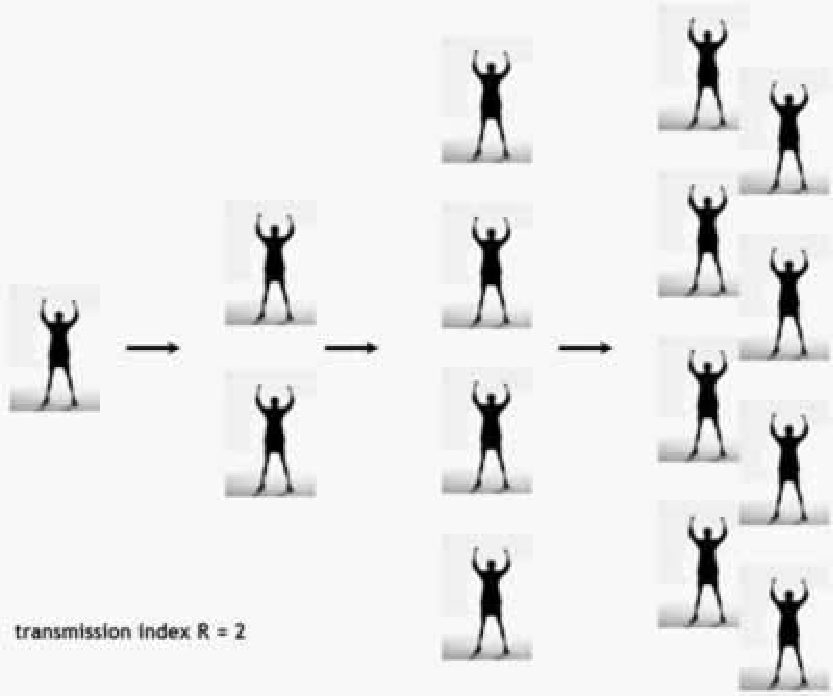
\includegraphics[width=.8\textwidth]{figs_steph/rzero}
\caption{Reproduction number $\mathcal{R}_0=2$.}
\end{figure}
Magnitude of the basic reproductive number gives an indication of the difficulty in controlling an epidemic or eradicating the disease: the larger the value of $\mathcal{R}_0$, the harder it is to control.



\section{SIS model without vital dynamics}
Consider a disease that confers no immunity. In this case,
individuals are either
\begin{itemize}
\item \emph{susceptible} to the disease, with the number of such individuals at time $t$ denoted by $S(t)$,
\item or \emph{infected} by the disease (and are also \emph{infective} in the sense that they propagate the disease), with the number of such individuals at time $t$ denoted by $I(t)$.
\end{itemize}
\vskip1cm
We want to model the evolution with time of $S$ and $I$ ($t$ is omitted unless necessary).

\frame{\frametitle{Hypotheses}
\begin{itemize}
\item Individuals recover from the disease at the \emph{per capita} rate $\gamma$.
\item The disease does not confer immunity.
\item There is no birth or death.
\item Infection is of \emph{standard incidence} type, $\beta=SI/N$.
\end{itemize}
(for details, see Chapter on \emph{residence time})
}


\begin{figure}[htbp]
\begin{center}    
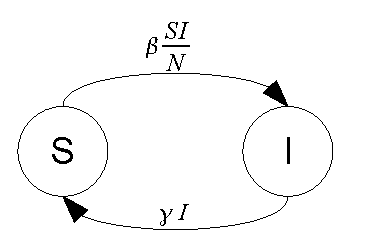
\includegraphics[width=0.4\textwidth]
{../figs_04_epidemic_models/SIS_nodemography}
\caption{Flow diagram of the model}
\end{center}
\end{figure}

The evolution of $I(t)$ is described by the following equation (see slides on \emph{residence time}):
\[
I'= \beta \frac{(N-I)I}{N}-\gamma I.
\]
Develop and reorder the terms, giving
\begin{equation}\label{sys:I_nodemography}
I'=(\beta-\gamma)I-\frac{\beta}{N} I^2
\end{equation}
This is a logistic-type equation. It can be solved as a Bernoulli equation or as a separable equation, giving, for an initial number of infectives $I(0)=I_0$,
\[
I(t)=\frac{(\beta-\gamma)NI_0}{(\beta-\gamma)Ne^{-(\beta-\gamma)t}+\beta I_0\left(1-e^{-(\beta-\gamma)t}\right)}
\]
From $S=N-I$, we deduce that the solution $(S(t),I(t))$ for the complete system, with initial condition $S(0)+I(0)=S_0+I_0=N$ is, for $t\geq 0$,
\[
S(t)=N-\frac{(\beta-\gamma)NI_0}{(\beta-\gamma)Ne^{-(\beta-\gamma)t}+\beta I_0\left(1-e^{-(\beta-\gamma)t}\right)}
\]
and 
\[
I(t)=\frac{(\beta-\gamma)NI_0}{(\beta-\gamma)Ne^{-(\beta-\gamma)t}+\beta I_0\left(1-e^{-(\beta-\gamma)t}\right)}
\]


\subsection{Behavior of the solutions}
Consider only $I$ for the moment.
\[
I(t)=\frac{{\red(\beta-\gamma)}NI_0}{{\red(\beta-\gamma)}Ne^{-{\red(\beta-\gamma)}t}+\beta I_0\left(1-e^{-{\red(\beta-\gamma)}t}\right)}
\]
So
\begin{itemize}
\item If $\beta-\gamma>0$, then $e^{-(\beta-\gamma)t}\to 0$ as $t\to\infty$, and therefore
\[
\lim_{t\to\infty} I(t)=\frac{(\beta-\gamma)NI_0}{\beta I_0}=\frac{\beta-\gamma}{\beta}N=\left(1-\frac{\gamma}{\beta}\right)N.
\]
\item If $\beta-\gamma<0$, then $e^{-(\beta-\gamma)t}\to\infty$ at $t\to\infty$. This implies that the denominator in $I(t)$ tends to $-\infty$ as $t\to\infty$, and so
\[
\lim_{t\to\infty} I(t)=0,\textrm{ with }I(t)>0\textrm{ for all }t.
\]
\item If $\beta=\gamma$, then $I(t)=0$ for all $t$.
\end{itemize}


\subsection{The basic reproduction number}
Define the \emph{basic reproduction number} (the average number of people that an infectious individual will infect, when introduced in a population of susceptibles) as 
\[
\Rzero=\frac\beta\gamma
\]
We have
\[
\left(\Rzero<1\Leftrightarrow (\beta-\gamma)<0\right)\textrm{ and }\left(\Rzero>1\Leftrightarrow (\beta-\gamma)>0\right).
\]
Therefore, previous cases can be rewritten
\begin{itemize}
\item If $\Rzero<1$, then $\lim_{t\to\infty}I(t)=0$.
\item If $\Rzero>1$, then
\[
lim_{t\to\infty} I(t)=\left(1-\frac{1}{\Rzero}\right)N.
\]
\end{itemize}
(The case $\Rzero=1$ is usually omitted.)
To plot this in Maple, use the commands
\mbox{}\newline
{\tt >} {\red\verb!f:=R->piecewise(R<1,0,R>1,(1-1/R)*1000);!}\\
{\tt >} {\red\verb!plot(f(R),R=0..10);!}
\newline
This gives the result shown in Figure~\ref{fig:bif_R0}.
\begin{figure}[htbp]
\begin{center}
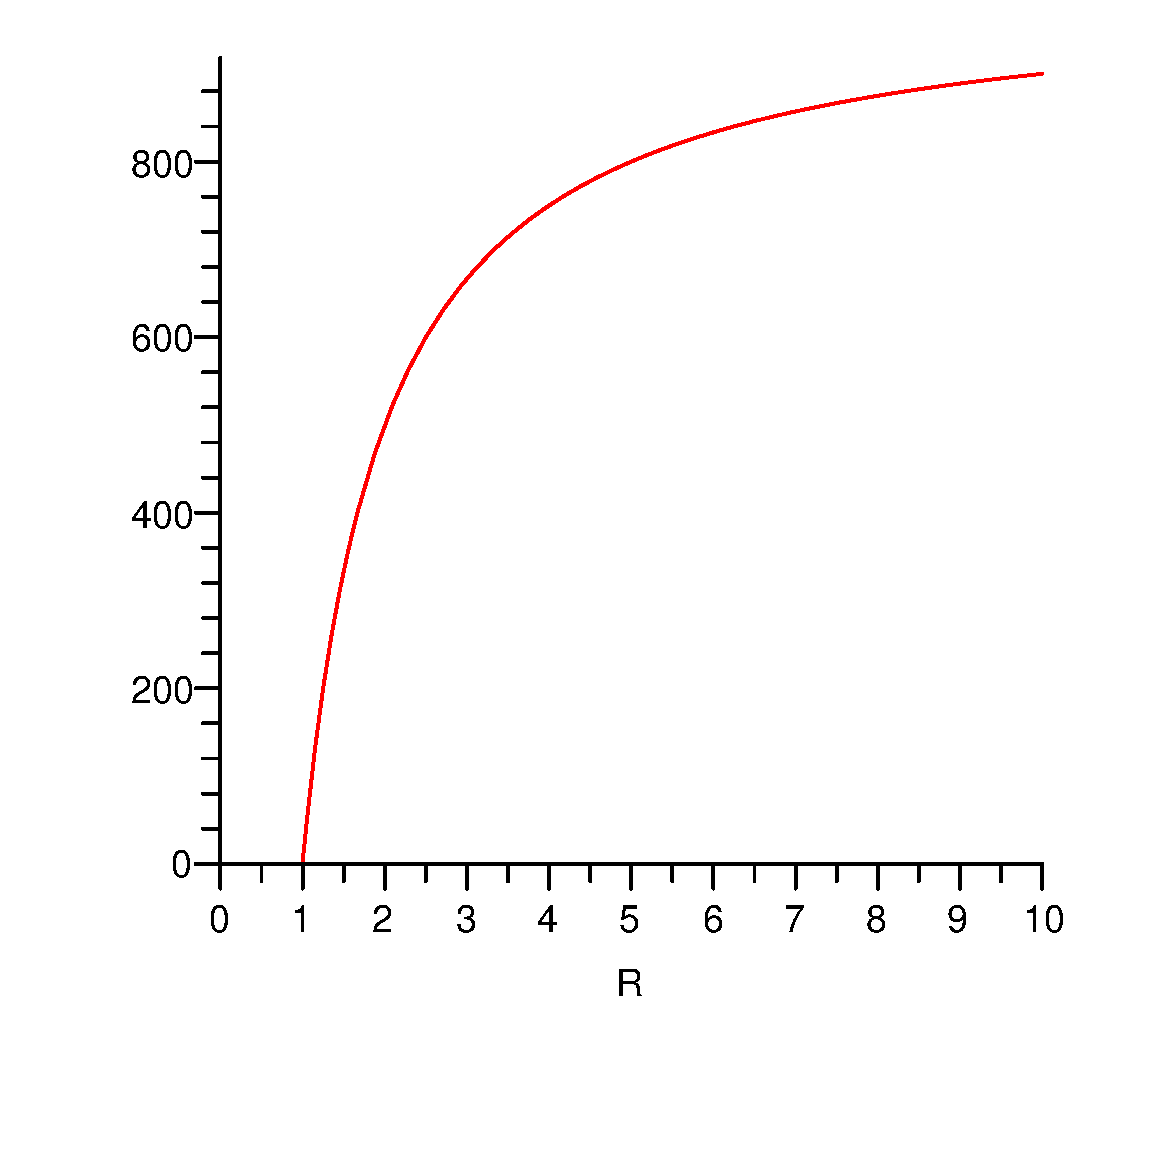
\includegraphics[width=0.45\textwidth]{../figs_04_epidemic_models/EEP_fct_R0}
\caption{Bifurcation diagram showing the number of infectives in the epidemic model, as a function of $\Rzero$.}
\label{fig:bif_R0}
\end{center}
\end{figure}




\section{SIR model of Kermack and McKendrick}

%\frame{
%\begin{center}
%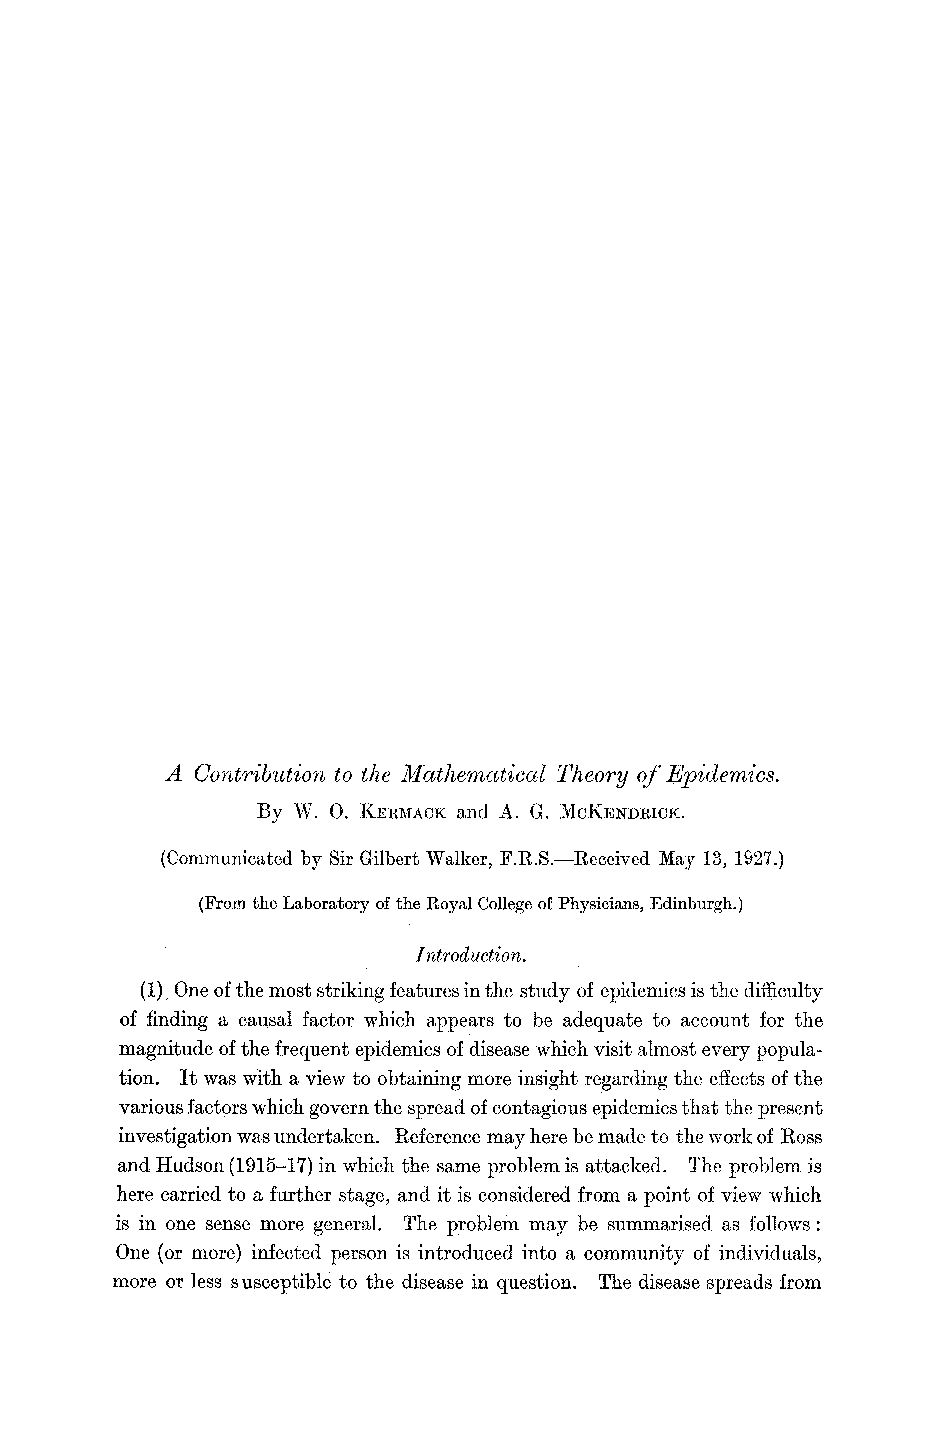
\includegraphics[width=0.7\textwidth]{../figs_04_epidemic_models/KMK_title}
%\end{center}
%}

%\begin{center}
%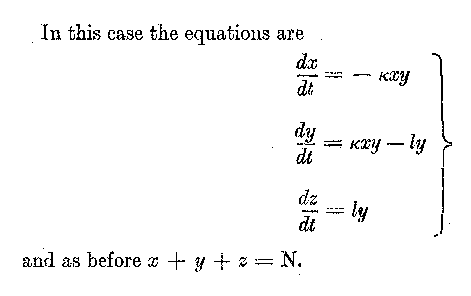
\includegraphics[width=0.7\textwidth]{../figs_04_epidemic_models/KMK_model1}
%\end{center}

In 1927, Kermack and McKendrick started publishing a series of papers on epidemic models \cite{KermackMckendrick1927,KermackMckendrick1932,KermackMckendrick1933}. In the first of their papers \cite{KermackMckendrick1927}, they have the following model as a particular case:
\begin{equation}\label{sys:KMK}
\begin{aligned}
S' &= -\beta SI \\
I' &= \beta SI-\gamma I \\
R' &= \gamma I
\end{aligned}
\end{equation}


% \begin{center}
% 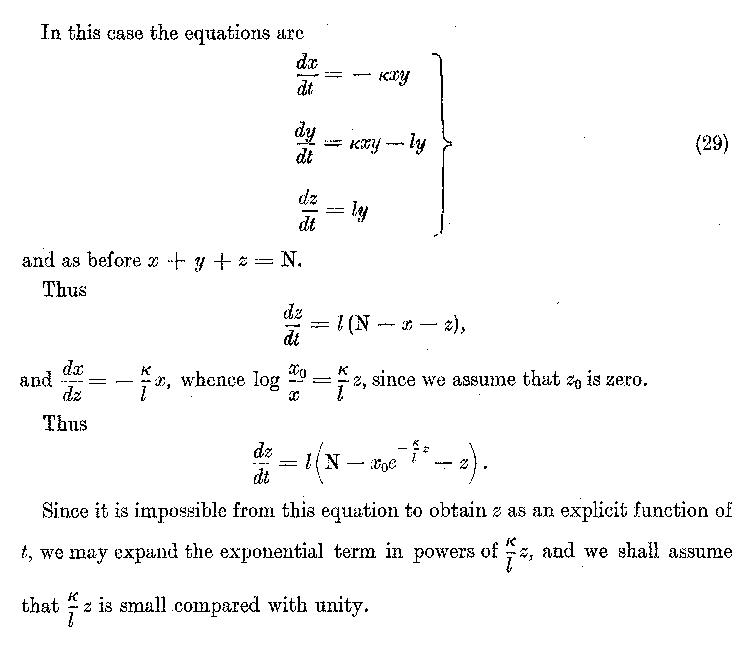
\includegraphics[width=\textwidth]{../figs_04_epidemic_models/KMK_model2}
% \end{center}

\frame{\frametitle{Analyzing the system}
First, note (as KMK) that the total population in the system is constant. This is deduced from the fact that
\[
N'=(S+I+R)'=-\beta SI+\beta SI-\gamma I+\gamma I=0.
\]
Since this is true for all values of $t$, we have $N$ constant.
}

\frame{
Let us ignore the $R$ equation for now.
We can compute
\[
\frac{dI}{dS}=\frac{dI}{dt}\frac{dt}{dS}=\frac{I'}{S'}=\frac{\gamma}{\beta S}-1
\]
This gives
\[
I(S)=S-\frac{\gamma}{\beta}\ln S+K,
\]
which, considering the initial condition $(S_0,I_0)$, is,
\[
I(S)=S-\frac{\gamma}{\beta}\ln S+I_0-(S_0-\frac{\gamma}{\beta}\ln S_0).
\]
This gives a curve in the $(S,I)$ plane.
}


\frame{
\[
I(S)=S-\frac{\gamma}{\beta}\ln S+I_0-(S_0-\frac{\gamma}{\beta}\ln S_0).
\]
Typically, assume $S\approx N$ and $I>0$ small.
Let us denote $S_\infty=\lim_{t\to\infty}S(t)$.

We want to find the value of $S$ when $I\to 0$.
Then
\[
I_0-\frac\gamma\beta\ln S_0=S_\infty -\frac\gamma\beta \ln S_\infty
\]
}

\section{SIRS models with demography}

\subsection{The SIRS model}
\begin{itemize}
\item Like KMK, individuals are S, I or R.
\item Infection is $\beta SI$ (mass action) or $\beta SI/N$ (proportional incidence).
\item Different interpretation of the R class: R stands for ``recovered'', individuals who are immune to the disease following recovery.
\item Recovery from the disease (movement from I class to R class) occurs at the per capita rate $\gamma$.\\ (Time spent in I before recovery is exponentially distributed.)
\item Immunity can be lost: after some time, R individuals revert back to S individuals.
\item Time spent in R class before loss of immunity is exponentially distributed, with mean $1/\nu$.
\item There is birth and death of individuals:
\begin{itemize}
\item No vertical transmission of the disease (mother to child) or of immunity, so all birth is into the S class.\\ Birth occurs at the rate $\Pi$.
\item Individuals in all classes die of at the per capita rate $d$, i.e., the average life duration is exponentially distributed with mean $1/d$.
\item The disease is lethal: infected individuals are subject to additional mortality at the per capita rate $\delta$.
\end{itemize}
\end{itemize}
Note that birth and death can have different interpretations:
\begin{itemize}
\item birth and death in the classical sense,
\item but also, entering the susceptible population and leaving it.
\end{itemize}

\begin{figure}[htbp]
\begin{center}
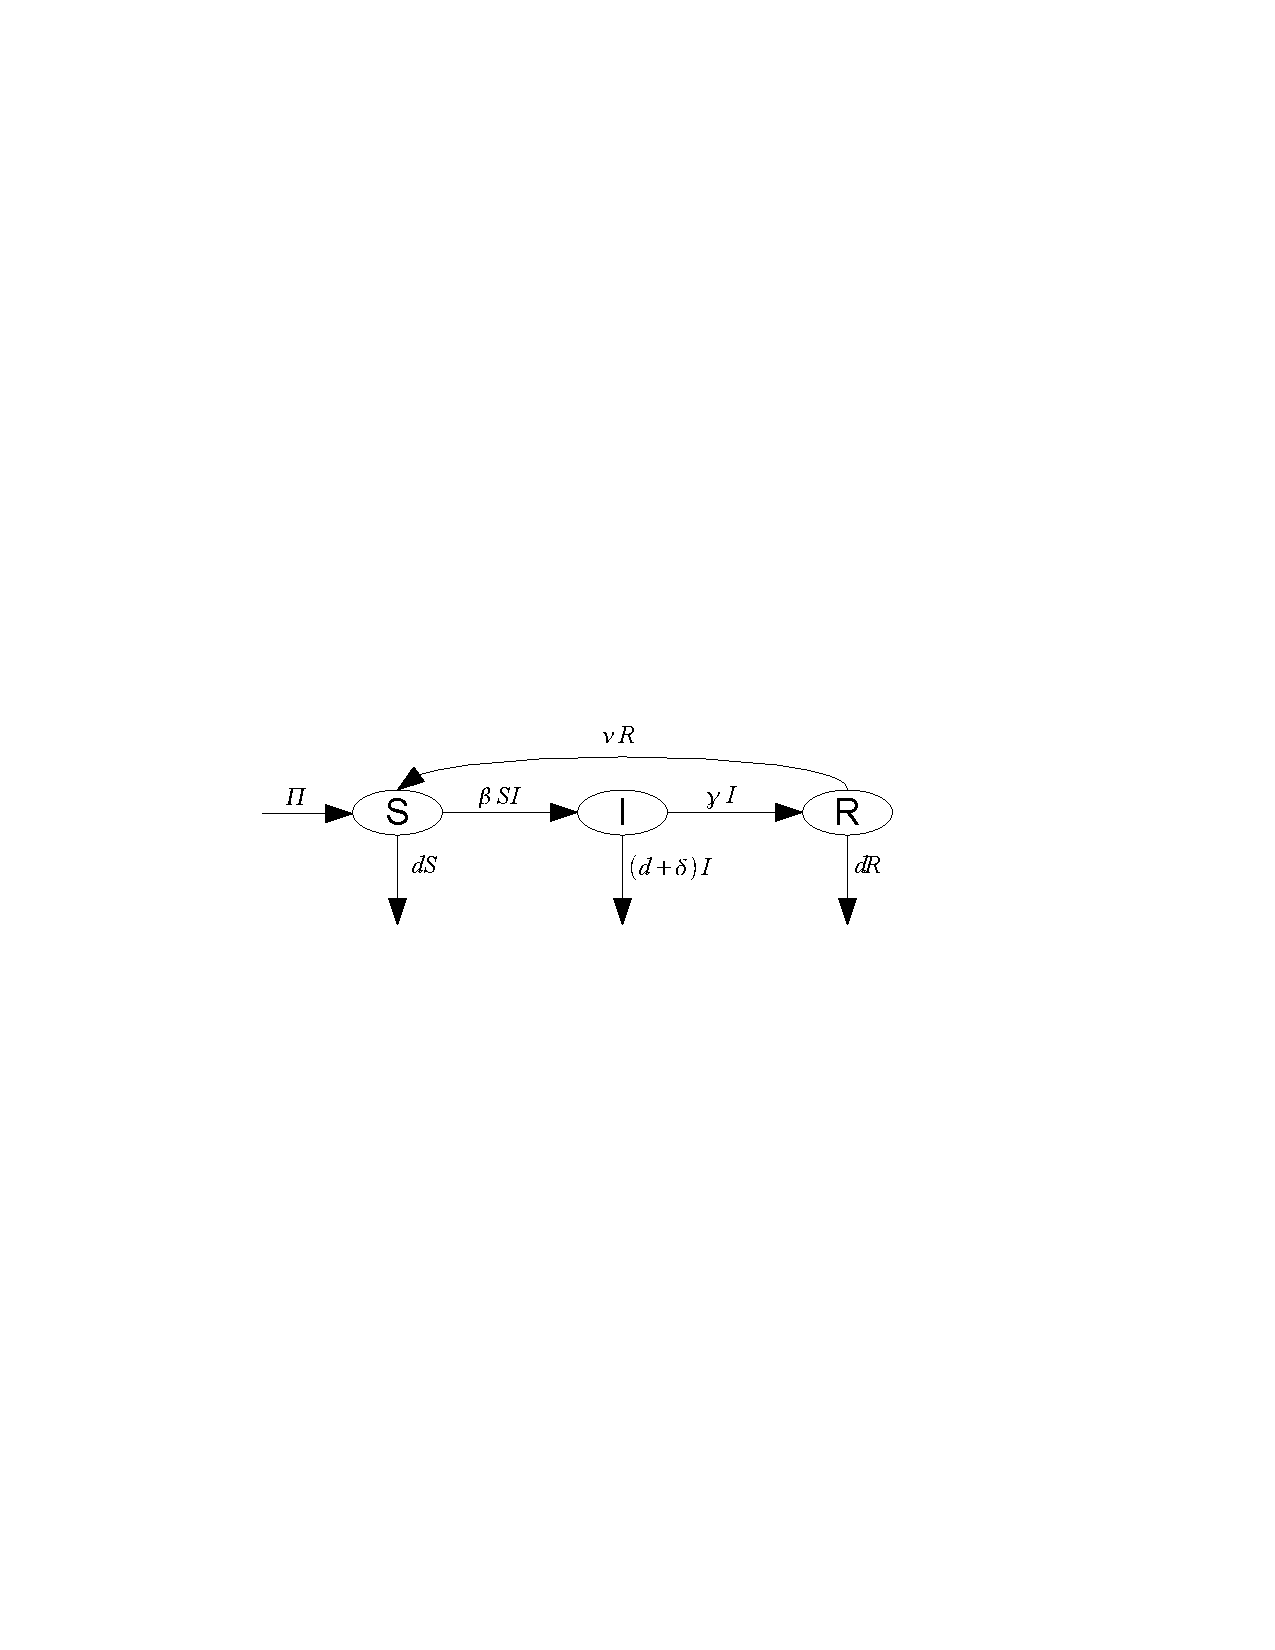
\includegraphics[width=0.45\textwidth]{../figs_04_epidemic_models/SIRS_massaction}
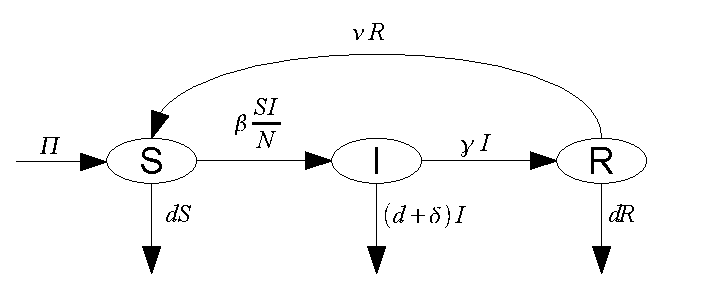
\includegraphics[width=0.45\textwidth]{../figs_04_epidemic_models/SIRS_propincidence}
\caption{The SIRS model with (left) mass action incidence and (right) proportional incidence.}
\end{center}
\end{figure}

\begin{description}
\item[Mass action]
\begin{subequations}\label{SIRS_MA}
\begin{align}
S' &= \Pi+\nu R-\beta SI-dS \label{SIRS_MA_S} \\
I' &= \beta SI-(d+\delta+\gamma)I \label{SIRS_MA_I} \\
R' &= \gamma I-(d+\nu)R \label{SIRS_MA_R}
\end{align}
\end{subequations}
\item[Proportional incidence]
\begin{subequations}\label{SIRS_P}
\begin{align}
S' &= \Pi+\nu R-\beta SI-dS \label{SIRS_P_S} \\
I' &= \beta SI-(d+\delta+\gamma)I \label{SIRS_P_I} \\
R' &= \gamma I-(d+\nu)R, \label{SIRS_P_R}
\end{align}
\end{subequations}
where $N=S+I+R$.
\end{description}
We consider \eqref{SIRS_MA}.

\subsection{Qualitative analysis}
\paragraph{Steps of the analysis}
\begin{enumerate}
\item Assess the well-posedness of the system:
\begin{enumerate}
\item Determine whether solutions exist and are unique.
\item Determine whether solutions remain in a realistic region and are bounded.
\end{enumerate}
\item Study the equilbrium solutions of the system:
\begin{enumerate}
\item Find the equilibria of the system.
\item Determine the local stability properties of the equilibria.
\item Determine the global stability properties of the equilibria ({\bf much harder}, often not possible).
\end{enumerate}
\item In the case of unstable equilibrium points, study the existence of periodic solutions.
\end{enumerate}


\paragraph{Existence and uniqueness of solutions}
\begin{theorem}[Cauchy-Lipschitz]
Consider the equation $x'=f(x)$, with $x\in\IR^n$, and suppose that $f\in C^1$. Then there exists a unique solution of $x'=f(x)$ such that $x(t_0)=x_0$, where $t_0\in\IR$ and $x_0\in\IR^n$, defined on the largest interval $J\ni t_0$ on which $f\in C^1$.
\end{theorem}



\begin{definition}[Equilibrium point]
Consider a differential equation
\begin{equation}\label{eq:ODE}
x'=f(x),
\end{equation}
with $x\in\IR^n$ and $f:\IR^n\to\IR^n$.
Then $x^*$ is an equilibrium (solution) of \eqref{eq:ODE} if $f(x^*)=0$.
\end{definition}

\paragraph{Linearization}
Consider $x^*$ an equilibrium of \eqref{eq:ODE}. For simplicity, assume here that $x^*=0$ (it is always possible to do this, by considering $y=x-x^*$).
Taylor's theorem:
\[
f(x)=Df(0)x+\frac 12 D^2f(0)(x,x)+\cdots,
\]
where $Df(0)$ is the Jacobian matrix of $f$ evaluated at $0$.


\frame{\frametitle{Stability of equilibria}
\begin{definition}[Stable and unstable EP]
Let $\phi_t$ be the flow of \eqref{eq:ODE}, assumed to be defined for all $t\in\IR$. An equilibrium $x^*$ of \eqref{eq:ODE} is (locally) \emph{stable} if for all $\varepsilon>0$, there exists $\delta>0$ such that for all $x\in\mathcal{N}_\delta(x^*)$ and $t\geq 0$, there holds
\[
\phi_t(x)\in\mathcal{N}_\varepsilon(x^*).
\]
The equilibrium point is \emph{unstable} if it is not stable.
\end{definition}
\begin{definition}[Asymptotically stable EP]
Let $\phi_t$ be the flow of \eqref{eq:ODE} is (locally) \emph{asymptotically stable} if there exists $\delta>0$ such that for all $x\in\mathcal{N}_\delta(x^*)$ and $t\geq 0$, there holds
\[
\lim_{t\to\infty}\phi_t(x)=x^*.
\]
\end{definition}
Clearly, Asymtotically Stable $\Rightarrow$ Stable.
}


\frame{\frametitle{Hyperbolic EPs, sinks, sources}
\begin{definition}[Sink]
An equilibrium point $x^*$ of \eqref{eq:ODE} is \emph{hyperbolic} if none of the eigenvalues of the matrix $Df(x^*)$ (Jacobian matrix of $f$ evaluated at $x^*$) have zero real parts.
\end{definition}
\begin{definition}[Sink]
An equilibrium point $x^*$ of \eqref{eq:ODE} is a \emph{sink} if all the eigenvalues of the matrix $Df(x^*)$ have negative real parts.
\end{definition}
\begin{definition}[Source]
An equilibrium point $x^*$ of \eqref{eq:ODE} is a \emph{source} if all the eigenvalues of the matrix $Df(x^*)$ have positive real parts.
\end{definition}
}

\frame{
\begin{theorem}
If $x^*$ is a sink of \eqref{eq:ODE} and for all the eigenvalues $\lambda_j$ of the matrix $Df(x^*)$
\[
\Re(\lambda_j)<-\alpha<0,
\]
where $\Re(\lambda)$ denotes the real part of $\lambda$, then for a given $\varepsilon>0$, there exists $\delta>0$ such that for all $x\in\mathcal{N}_\delta(x^*)$, the flow $\phi_t(x)$ of \eqref{eq:ODE} satisfies
\[
\|\phi_t(x)-x^*\|\leq\varepsilon e^{-\alpha t}
\]
for all $t\geq 0$.
\end{theorem}
\begin{theorem}
If $x^*$ is a stable equilibrium point of \eqref{eq:ODE}, no eigenvalue of $Df(x^*)$ has positive real part.
\end{theorem}
}
\chapter[Chemostat]{The chemostat\\[0.5cm] Some notions of phase plane analysis}
\label{chap:chemostat}



\section{The chemostat}

A chemostat consists in one main chamber (called a vessel), in which some microorganisms (bacteria, plankton), typically unicellular, are put, together with liquid and nutrient.
The contents are stirred, so nutrient and organisms are well-mixed.
Organisms consume the nutrient in their environment, which causes them to grow and multiply.
\begin{figure}[htbp]
\begin{center}
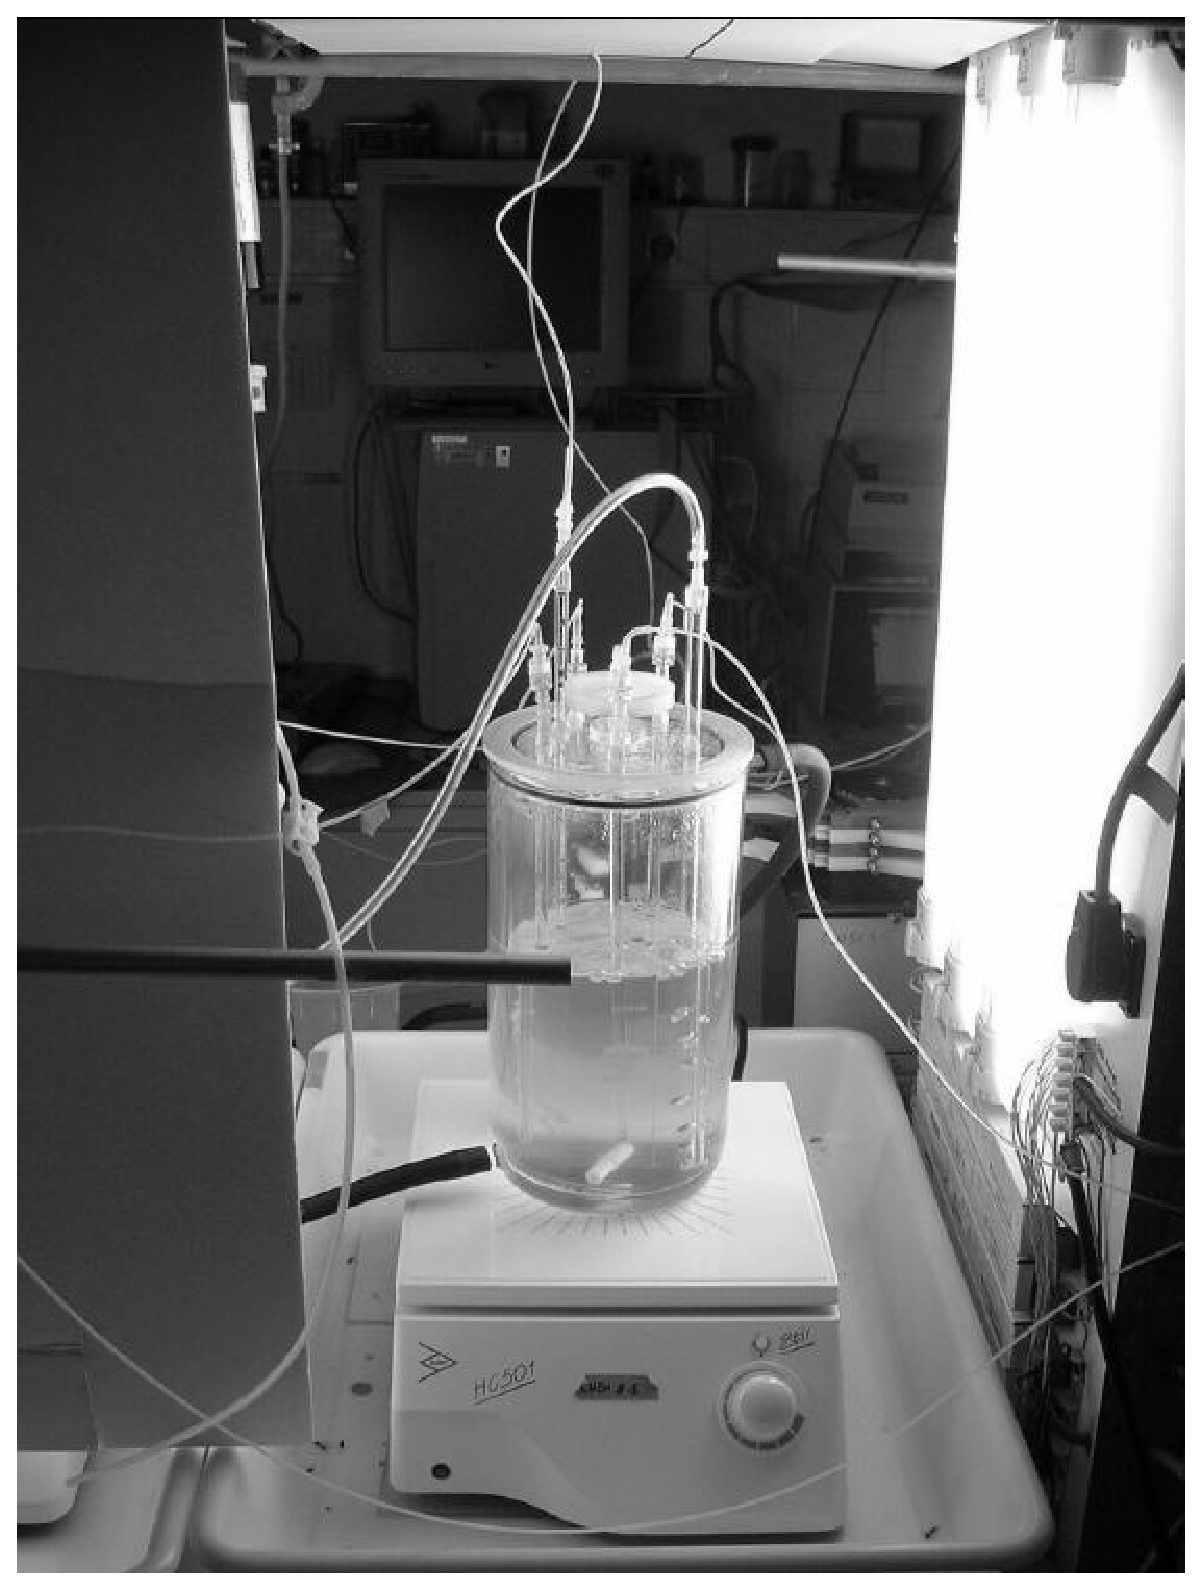
\includegraphics[height=0.45\textheight]
{../figs_05_chemostat/chemostat}
\caption{A chemostat operating at the Laboratoire
Oc\'eanographique de Villefranche sur Mer, France.}
\end{center}
\end{figure}
Two major modes of operation:
\begin{itemize}
\item \emph{Batch} mode: let the whole thing sit.
\item \emph{Continuous flow} mode: there is an input of fresh water and nutrient, and an outflow the comprises water, nutrient and organisms, to keep the volume constant.
\end{itemize}
Chemostats are very popular tools.
\begin{itemize}
\item Study of the growth of micro-organisms as a function of nutrient, in a very controlled setting.
\item Very good reproducibility of experiments.
\item Used in all sorts of settings. Fundamental science, but also, for production of products.
\end{itemize}


\section{Batch mode}
\subsection{Model with no cell mortality}
We make the following assumptions. Organisms, whose concentration is denoted $x$, are in the main vessel. Limiting substrate has a concentration in the vessel denoted $S$. There is homogeneous mixing of the contents of the vessel, so that nutrient is readily available to all organisms at the same  concentration. Therefore, spatial aspects can be neglected. Organisms uptake nutrient at the rate $\mu(S)$, a function of the concentration of nutrient around them.
First, we assume no death of organisms. The model then is
\begin{subequations}\label{sys:chemo_batch_nodeath}
\begin{align}
S' &= -\mu(S)x \\
x' &= \mu(S)x
\end{align}
\end{subequations}
with initial conditions $S(0)\geq 0$ and $x(0)>0$, and
where $\mu(S)$ is such that
\begin{itemize}
\item $\mu(0)=0$ (no substrate implies no growth)
\item $\mu(S)\geq 0$ for all $S\geq 0$
\item $\mu(S)$ bounded for $S\geq 0$
\end{itemize}
A typical form for $\mu(S)$ is the \emph{Monod} curve,
\begin{equation}\label{eq:monod}
\mu(S)=\mu_{max}\frac S{K_S+S}.
\end{equation}
The parameter $\mu_{max}$ is the \emph{maximal growth rate}, while $K_S$ is
the half-saturation constant ($\mu(K_S)=\mu_{max}/2$). See an example in
Figure~\ref{fig:monod_curve}.
\begin{figure}[htbp]
\begin{center}
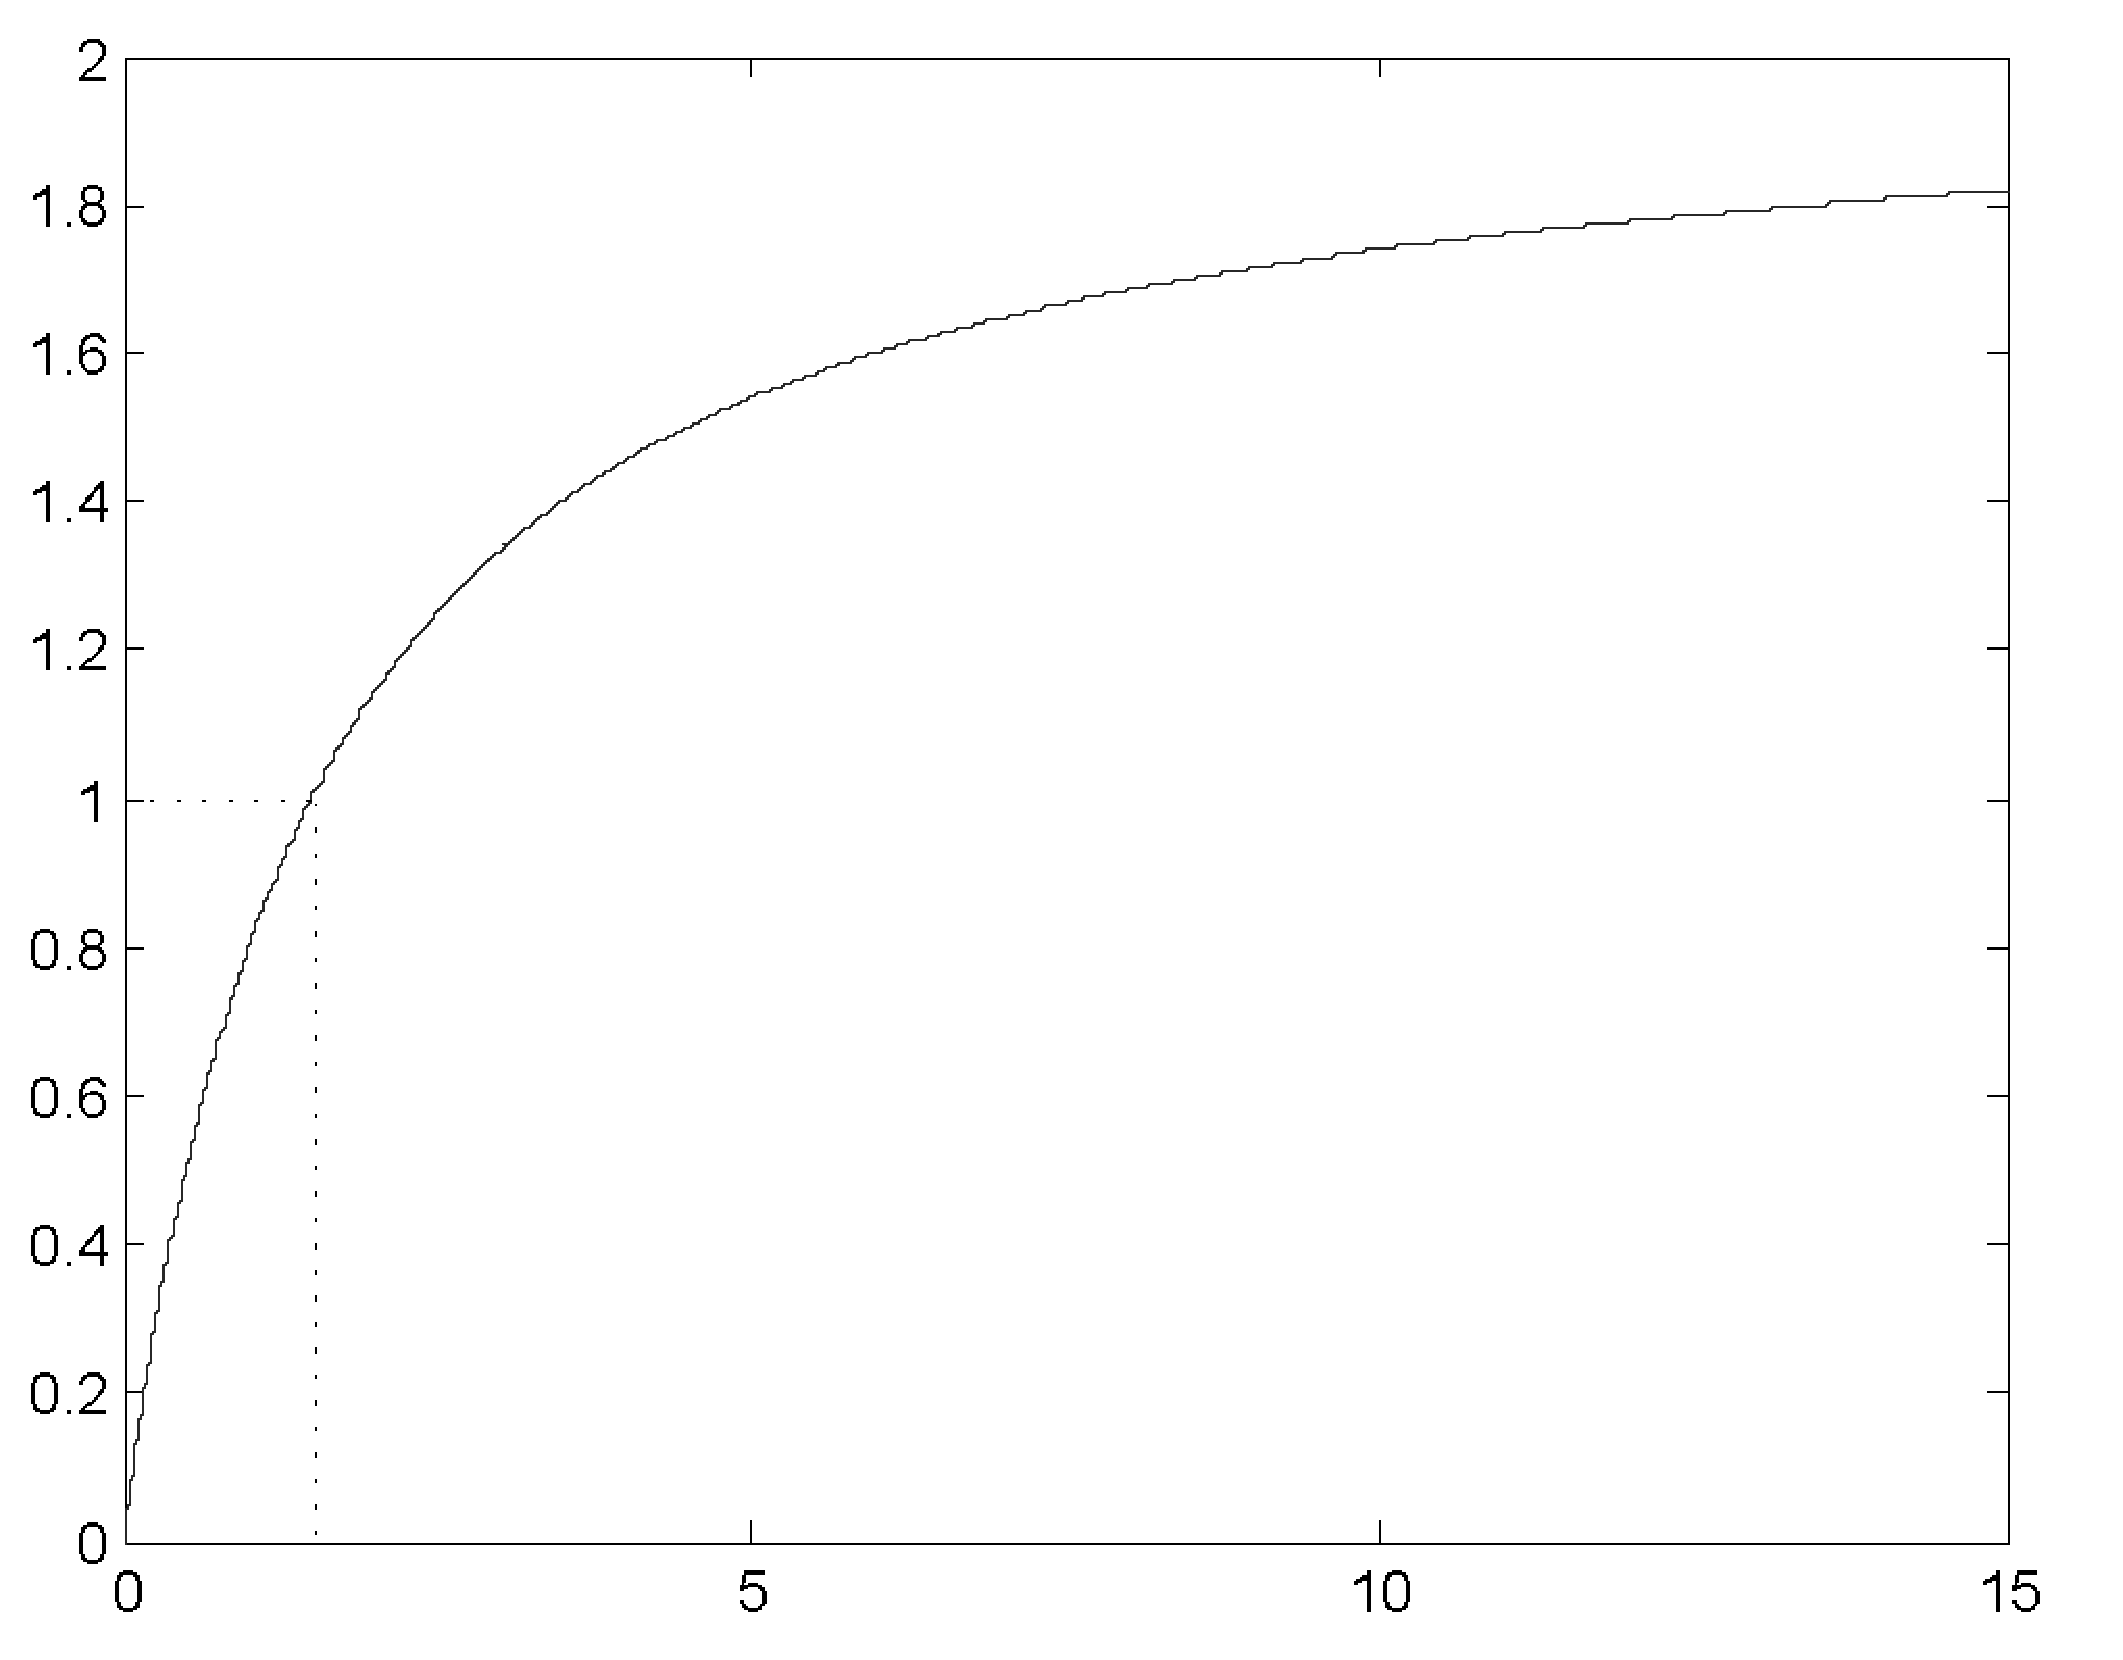
\includegraphics[width=0.5\textwidth]{../figs_05_chemostat/monod}
\caption{A typical Monod growth curve.}
\end{center}
\label{fig:monod_curve}
\end{figure}
From now on, we assume a Monod function. 
In other contexts, this curve is called a Holling Type II function.


\subsection{Equilibria}
To compute the equilibria, suppose $S'=x'=0$, giving
\[
\mu(S)x=-\mu(S)x=0.
\]
This implies $\mu(S)=0$ or $x=0$. Note that $\mu(S)=0\Leftrightarrow S=0$, so the system is at equilibrium if $S=0$ or $x=0$.

This is a complicated situation, as it implies that there are lines of
equilibria ($S=0$ and any $x$, and $x=0$ and any $S$), so that the equilibria
are not \emph{isolated} (arbitrarily small neighborhoods of one equilibrium
contain other equilibria), and therefore, studying the linearization is not
possible.
Here, some analysis is however possible.
Consider
\[
\frac{dx}{dS}=\frac{dx}{dt}\frac{dt}{dS}=-\frac{\mu(S)x}{\mu(S)x}=-1.
\]
This implies that we can find the solution
\[
x(S)=C-S,
\]
or, supposing the initial condition is $(S(0),x(0))=(S_0,x_0)$, that is, $x(S_0)=x_0$,
\begin{equation}\label{eq:sol_chemostat_batch_no_death}
x(S)=S_0+x_0-S.
\end{equation}
\begin{figure}[htbp]
\begin{center}
\includegraphics[width=0.5\textwidth]
{../figs_05_chemostat/chemo_batch_nodeath_Sx}
\caption{Typical solutions obtained from
\eqref{eq:sol_chemostat_batch_no_death}.}
\end{center}
\end{figure}




\subsection{Model with organism death}
Assume death of organisms at per capita rate $d$. Model is
\begin{subequations}\label{sys:chemo_batch_death}
\begin{align}
S' &= -\mu(S)x \\
x' &= \mu(S)x-dx.
\end{align}
\end{subequations}
We have
\[
S'=0\Leftrightarrow \mu(S)x=0
\]
and
\[
x'=0\Leftrightarrow (\mu(S)-d)x=0.
\]
So we have $x=0$ or $\mu(S)=d$. So $x=0$ and any value of $S$, and $S$ such that $\mu(S)=d$ and $x=0$. One such particular value is $(S,x)=(0,0)$.
This is once again a complicated situation, since there are lines of equilibria. Intuitively, most solutions will go to $(0,0)$. This is indeed the case (we will not show it).



\section{Continous flow mode}
\subsection{Modelling principles}
General hypotheses are similar to the batch case, except that additionally,
\begin{itemize}
\item Limiting substrate (whose concentration in the vessel is denoted $S$) is input at the rate $D$ and concentration $S^0$.
\item There is an outflow of both nutrient and organisms (at same rate $D$ as input). 
\item Residence time in device is assumed small compared to lifetime (or time to division) $\Rightarrow$ no death considered.
\end{itemize}

\begin{figure}[htbp]
\begin{center}
\includegraphics[height=0.45\textwidth]{../figs_05_chemostat/figchemo_eng}
\caption{A schematic representation of a chemostat operating in continuous flow
mode.}
\label{fig:schema_chemostat_CSTR}
\end{center}
\end{figure}


\subsection{Model for continuous flow mode}
The model is
\begin{subequations}\label{sys:chemo_flow}
\begin{align}
S' &= D(S^0-S)-\mu(S)x \\
x' &= \mu(S)x-Dx,
\end{align}
\end{subequations}
with initial conditions $S(0)\geq 0$ and $x(0)\geq 0$, and $D,S^0>0$. This is called the \emph{Monod model}.


\subsection{Finding equilibria}
Setting $S'=x'=0$, we get
\begin{align*}
0&=D(S^0-S)-\mu_{max}\frac{S}{K_S+S}x \\
0&=\left(\mu_{max}\frac{S}{K_S+S}-D\right)x
\end{align*}
But here, instead of directly computing the values of the equilibrium points, we consider the system in the plane, using nullclines.


\subsection{Phase plane analysis}
Nullclines are the level set 0 of the vector field. If we have
\begin{align*}
x_1' &= f_1(x_1,x_2) \\
x_2' &= f_2(x_1,x_2)
\end{align*}
then the nullclines for $x_1$ are the curves defined by 
\[
\{(x_1,x_2)\in\IR^2:f_1(x_1,x_2)=0\},
\]
those for $x_2$ are
\[
\{(x_1,x_2)\in\IR^2:f_2(x_1,x_2)=0\}.
\]
(Note: In $\IR^2$, nullclines are curves.)
On the nullcline associated to one state variable, this state variable has zero derivative.
Equilibria lie at the intersections of nullclines for both state variables (in $\IR^2$).

\frame{\frametitle{Nullclines for $x$}
Nullclines are given by
\begin{subequations}
\begin{align}
0&=D(S^0-S)-\mu_{max}\frac{S}{K_S+S}x \label{eq:ncS}\\
0&=\left(\mu_{max}\frac{S}{K_S+S}-D\right)x \label{eq:ncx}
\end{align}
\end{subequations}
From \eqref{eq:ncx}, nullclines for $x$ are $x=0$ and 
\[
\mu_{max}\frac{S}{K_S+S}-D=0
\]
Write the latter as
\begin{align*}
\mu_{max}\frac{S}{K_S+S}-D=0 &\Leftrightarrow \mu_{max}S=D(K_S+S) \\
&\Leftrightarrow (\mu_{max}-D)S=DK_S \\
&\Leftrightarrow S=\frac{DK_S}{\mu_{max}-D}
\end{align*}
}

\frame{\frametitle{Nullcline for $x$}
So, for $x$, there are two nullclines:
\begin{itemize}
\item The line $x=0$.
\item The line $S=\dfrac{DK_S}{\mu_{max}-D}$.
\end{itemize}
For the line $S=DK_S/(\mu_{max}-D)$, we deduce a condition:
\begin{itemize}
\item If $\mu_{max}-D>0$, that is, if $\mu_{max}>D$, i.e., the maximal growth rate of the cells is larger than the rate at which they leave the chemostat due to washout, then the nullcline intersects the first quadrant.
\item If $\mu_{max}<D$, then the nullcline does not intersect the first quadrant. 
\end{itemize}
}

\frame{\frametitle{Nullclines for $S$}
Nullclines are given by
\begin{subequations}
\begin{align}
0&=D(S^0-S)-\mu_{max}\frac{S}{K_S+S}x \tag{\ref{eq:ncS}}\\
0&=\left(\mu_{max}\frac{S}{K_S+S}-D\right)x \tag{\ref{eq:ncx}}
\end{align}
\end{subequations}
Rewrite \eqref{eq:ncS},
\begin{align*}
D(S^0-S)-\mu_{max}\frac{S}{K_S+S}x=0 &\Leftrightarrow 
\mu_{max}Sx=D(S^0-S)(K_S+S) \\
&\Leftrightarrow 
x = \frac{D(S^0-S)(K_S+S)}{\mu_{max}S}
\end{align*}
}


\frame{\frametitle{Nullcline for $S$: $S$ intercept}
The equation for the nullcline for $S$ is
\[
x =\Gamma(S)\stackrel{\Delta}{=} \frac{D}{\mu_{max}}\left(\frac{S^0K}S-S+S^0-K\right)
\]
We look for the intercepts. First, $S$ intercept:
\begin{align*}
\Gamma(S)=0 &\Leftrightarrow \frac{S^0K_S}S-S+S^0-K_S=0 \\
&\Leftrightarrow \frac{S^0K}S=S-S^0+K \\
&\Leftrightarrow S^0K_S=S^2+(K_S-S^0)S \\
&\Leftrightarrow S^2+(K-S^0)S-S^0K_S =0
\end{align*}
Roots of this degree 2 polynomial are $-K_S$ ($<0$) and $S^0$.
}

\paragraph{Nullcline for $S$: $x$ intercept}
$x$ intercept is found at $\Gamma(0)$. But this is not defined (division by $S=0$), so consider
\begin{align*}
\lim_{S\to 0^+}\Gamma(S) &= \lim_{S\to 0^+}\frac{D}{\mu_{max}}\left(\frac{S^0K}S-S+S^0-K\right) \\
&= \frac{D}{\mu_{max}}\left(\lim_{S\to 0^+}\frac{S^0K}S-S+S^0-K\right) \\
&= \frac{D}{\mu_{max}}\left(\lim_{S\to 0^+}\left(\frac{S^0K}S\right)+\lim_{S\to 0^+}\left(-S+S^0-K\right)\right) \\
&= \frac{D}{\mu_{max}}\left(+\infty+S^0-K\right) \\
&= +\infty.
\end{align*}


Maple has a plot function, {\tt implicitplot} (part of the {\tt plots} library), that is very useful for nullclines ($d$ is used instead of $D$, because maple does not allow to change $D$ without using {\tt unprotect}).
\begin{verbatim}
> with(plots):
> d := 0.4; S0 := 1; mu := 0.7; K := 2;
> implicitplot(d*(S0-S)-mu*S/(K+S)*x=0,S=0..10,x=0..10)
\end{verbatim}



\subsection{Stability of the equilibria}
The computation was done during class.


\subsection{Conservation of mass}
Summing the equations in \eqref{sys:chemo_flow}, we get
\[
(S+x)'=D\left(S^0-(S+x)\right)
\]
Denote $M=S+x$ the total organic mass in the chemostat. Then
\[
M'=D(S^0-M)
\]
This is a linear equation in $M$. Solving it (e.g., integrating factor), we find
\[
M(t)=S^0-e^{-Dt}\left(S^0-M(0)\right),
\]
and so
\[
\lim_{t\to\infty}M(t)=S^0.
\]
This is called the \emph{mass conservation principle}.

\paragraph{Implication of mass conservation}
Not as strong as what we had in the SIS epidemic model, where the total number of individuals was constant. Here, the mass is \emph{asymptotically} constant.
{\bf But} we can still use it, using the theory of \emph{asymptotically autonomous} differential equations. Too complicated for here, just remember that often, it is \emph{allowed} to use the limit of a variable rather than the variable itself, provided you know that the convergence occurs.


\chapter[Traffic flow]{Traffic flow\\[0.5cm] Linear cascades\\ Linear systems\\
Delay differential equations\\ Laplace transform}
\label{chap:traffic_flow}



\section{An ODE model of traffic flow}

We want to model a situation with $N$ cars on a straight road with no overtaking, and where a given driver adjusts (instantaneously) their speed on the speed the driver in front of them.
\subsection{Hypotheses}
\begin{itemize}
\item $N$ cars in total,
\item the road is the $x$-axis,
\item $x_n(t)$ is the position of the $n$th car at time $t$,
\item $v_n(t)\stackrel{\Delta}{=}x_n'(t)$ is the velocity of the $n$th car at time $t$,
\item all cars start with the same initial speed $v_0$ at time $t=0$.
\end{itemize}
\begin{figure}[htbp]
\begin{center}
\includegraphics[width=0.8\textwidth]{../figs_06_traffic_flow/traffic_flow1}
\caption{The situation described by the model of traffic flow.}
\label{fig:traffic_flow_ODEmodel}
\end{center}
\end{figure}
To make computations easier, we express the velocity of cars in a reference frame
moving at the speed $u_0$. (Remark that here, speed and velocity are equal, since movement is 1-dimensional.)
Let
\[
u_n(t)=v_n(t)-u_0.
\]
Then $u_n(t)=0$ for $t\leq 0$, and $u_n$ is the speed of the $n$th car in the moving frame coordinates.


\subsection{Modeling driver behavior}
Assume that a driver adjusts their speed according to relative speed between their car and the car in front, and that this adjustment is a linear term, equal to $\lambda$ for all drivers. This implies the following.
\begin{itemize}
\item
For the first car, the evolution of speed remains to be determined.
\item 
For the second car,
\[
u_2'=\lambda(u_1-u_2).
\]
This means that if the speed of the second car, $u_2$, is larger than that of the first car, $u_1$, then the driver of the second car decreases their speed ($u_2'$ has a negative sign). Similarly, if the speed of the second car is smaller than that of the first car, then the term $\lambda(u_2-u_1)$ is positive, implying that $u_2'>0$, i.e., the second car speeds up.
\item
Similarly, the third car adjusts its speeds as a function of the car in front, i.e., car number 2, giving
\[
u_3'=\lambda(u_2-u_3).
\]
\item 
Thus, for $n=1,\ldots,N-1$,
\begin{equation}\label{eq:ode_traffic_flow}
u_{n+1}'=\lambda(u_n-u_{n+1}).
\end{equation}
\end{itemize}

\subsection{Solving using linear cascades}
This can be solved using \emph{linear cascades}: if $u_1(t)$ is known, then
\[
u_2'=\lambda(u_1(t)-u_2)
\]
is a linear first-order nonhomogeneous equation. The solution (obtained using integrating factors or variation of constants) is
\[
u_2(t)=\lambda e^{-\lambda t}\int_0^t u_1(s)e^{\lambda s}ds.
\]
Then use this function $u_2(t)$ in $u_3'$ to get $u_3(t)$,
\begin{align*}
u_3(t) &= \lambda e^{-\lambda t}\int_0^t u_2(s)e^{\lambda s}ds.
\end{align*}
Thus
\begin{align*}
u_3(t) &= \lambda e^{-\lambda t}\int_0^t u_2(s)e^{\lambda s}ds \\
&= \lambda e^{-\lambda t}\int_0^t 
\left(\lambda e^{-\lambda s}\int_0^s u_1(q)e^{\lambda q}dq\right)ds \\
&= \lambda^3 e^{-\lambda t}\int_0^t e^{-\lambda s}\int_0^s u_1(q)e^{\lambda q}dqds.
\end{align*}
Continue the process to get the solution.

\subsection{An example with known first driver behavior}
Suppose that the driver of car 1 follows the function
\[
u_1(t)=\alpha\sin(\omega t),
\]
that is, $\omega$-periodic, 0 at $t=0$ (we want all cars to start with speed relative to the moving reference frame equal to 0), and with amplitude $\alpha$.
Then
\begin{align*}
u_2(t) &= \lambda\alpha e^{-\lambda t}\int_0^t \sin(\omega s)e^{\lambda s}ds \\
&= \lambda\alpha e^{-\lambda t}
\left(
\frac{\omega-\omega e^{\lambda t} \cos(\omega t)+\lambda e^{\lambda t} \sin(\omega t)}{\lambda^2+\omega^2}
\right) \\
&= \frac{\lambda\alpha}{\lambda^2+\omega^2}\left(\omega e^{-\lambda t}
+\lambda\sin(\omega t)-\omega\cos(\omega t)\right).
\end{align*}
When $t\to\infty$, the first term goes to 0 and we are left with a $\omega$-periodic
term.
Continuing the process,
\[
u_3(t) = \frac{\lambda^2\alpha}{\lambda^2+\omega^2} e^{-\lambda t}
\int_0^t \left(\omega e^{-\lambda s}
+\lambda\sin(\omega s)-\omega\cos(\omega s)\right)e^{\lambda s}ds,
\]
that is,
\begin{align*}
u_3(t) &= \frac{\lambda^2\alpha}{\lambda^2+\omega^2}e^{-\lambda t}\left(\omega t+\int_0^t \left(\lambda\sin(\omega s)-\omega\cos(\omega s)\right)e^{\lambda s}ds\right) \\
&= \frac{\lambda^2\alpha}{\lambda^2+\omega^2}\left(\omega t+\frac{2 \lambda \omega}{\lambda^2+\omega^2}\right)e^{-\lambda t}\\
&\quad -\frac{\lambda^2\alpha}{(\lambda^2+\omega^2)^2}\left(2 \lambda \omega \cos(\omega t)-\lambda^2 \sin(\omega t)+\omega^2 \sin(\omega t)\right).
\end{align*}
Once again, the terms in $e^{-\lambda t}$ vanishes for large $t$, and we are left with 3 $\omega$-periodic terms.




\section{Linear systems -- Our case}
\subsection{General computations, case of 3 cars}
We consider the case of 3 cars. Let
\[
X=\begin{pmatrix}
u_2\\ u_3
\end{pmatrix}
\]
Then the system can be written as
\[
X'=\begin{pmatrix}
-\lambda & 0 \\
\lambda & -\lambda
\end{pmatrix}X
+\begin{pmatrix}
\lambda u_1(t)\\ 0
\end{pmatrix}
\]
which we write for short as $X'=AX+B(t)$.
The matrix $A$ has the eigenvalue $-\lambda$ with multiplicity 2. Its Jordan form can be obtained using the maple function {\tt JordanForm}:
\begin{verbatim}
> with(LinearAlgebra)
> A := <<-lambda, lambda> | <0, -lambda>>:
> J := JordanForm(A)
\end{verbatim}
giving
\[
J=\begin{pmatrix}
-\lambda & 1 \\
0 & -\lambda
\end{pmatrix}
\]
To get the matrix of change of basis, 
\begin{verbatim}
> P := JordanForm(A,output='Q')
\end{verbatim}
giving
\[
P=\begin{pmatrix}
0 & 1 \\
\lambda & 0
\end{pmatrix}
\]
which is such that $P^{-1}AP=J$.
Because $-\lambda$ is an eigenvalue with multiplicity 2 (the same multiplicity as as the size of the matrix), we can use the simplified theorem Theorem~\ref{th:Jordan_simple_case}, and only need $N$. 
We have
\begin{align*}
N &= A-S \\
&=\begin{pmatrix}
-\lambda & 0 \\
\lambda & -\lambda
\end{pmatrix}
-
\begin{pmatrix}
-\lambda & 0 \\
0 & -\lambda
\end{pmatrix} \\
&=\begin{pmatrix}
0 & 0 \\
\lambda & 0
\end{pmatrix}.
\end{align*}
Clearly, $N^2=0$, so, by the theorem in the simplified case,
\begin{align*}
x(t) &= e^{-\lambda t}\left(\II+Nt\right)x_0 \\
\end{align*}
But we know that solutions are unique, and that the solution to the differential equation is given by $x(t)=e^{At}x_0$. This means that
\begin{align*}
e^{At} &= e^{-\lambda t}\left(\II+Nt\right)\\
&= e^{-\lambda t}\left(\begin{pmatrix}1&0\\0&1\end{pmatrix}+
\begin{pmatrix}
0 & 0 \\
\lambda t & 0
\end{pmatrix}\right)\\
&= e^{-\lambda t}\begin{pmatrix}
1 & 0 \\
\lambda t & 1
\end{pmatrix} \\
&= \begin{pmatrix}
e^{-\lambda t} & 0 \\
\lambda te^{-\lambda t} & e^{-\lambda t}
\end{pmatrix}.
\end{align*}
Now notice that the solution to
\[
X'=AX
\]
is trivially established here, since
\[
X(0)=\begin{pmatrix}u_2(0)\\u_3(0)\end{pmatrix}=\begin{pmatrix}0\\0\end{pmatrix},
\]
and thus
\[
X(t)=e^{At}0=0.
\]
The matrix $e^{At}$ does however play a role in the solution (fortunately), since it is involved in the variation of constants formula:
\[
X(t)=e^{At}X_0+\int_0^t e^{A(t-s)}B(s)ds.
\]
Thus we need to compute $e^{A(t-s)}B(s)$, and then the integral.
\begin{align*}
e^{A(t-s)}B(s) &= 
\begin{pmatrix}
e^{-\lambda (t-s)} & 0 \\
\lambda (t-s)e^{-\lambda (t-s)} & e^{-\lambda (t-s)}
\end{pmatrix}
\begin{pmatrix}
\lambda u_1(s)\\ 0
\end{pmatrix} \\
&= \begin{pmatrix}
\lambda e^{-\lambda(t-s)}u_1(s) \\
\lambda^2e^{-\lambda(t-s)} (t-s)u_1(s)
\end{pmatrix}
\end{align*}
and thus
\begin{align*}
\int_0^t e^{A(t-s)}B(s)ds &=
\int_0^t\left(
\begin{array}{ll}
\lambda e^{-\lambda(t-s)}u_1(s) \\
\lambda^2e^{-\lambda(t-s)} (t-s)u_1(s)
\end{array}
\right)ds \\
&= \left(\begin{array}{ll}
\int_0^t\lambda e^{-\lambda(t-s)}u_1(s) ds \\
\int_0^t\lambda^2e^{-\lambda(t-s)} (t-s)u_1(s) ds
\end{array}
\right) \\
&= \left(\begin{array}{ll}
\lambda e^{-\lambda t} \int_0^te^{\lambda s}u_1(s) ds \\
\lambda^2 e^{-\lambda t}\int_0^te^{\lambda s} (t-s)u_1(s) ds
\end{array}
\right) \\
&= \left(\begin{array}{ll}
\lambda e^{-\lambda t} \int_0^te^{\lambda s}u_1(s) ds \\
\lambda^2 e^{-\lambda t}\left(t\int_0^te^{\lambda s}u_1(s) ds
-\int_0^tse^{\lambda s} u_1(s) ds\right)
\end{array}
\right).
\end{align*}
Let
\[
\Psi(t)=\int_0^t e^{\lambda s} u_1(s)ds
\]
and
\[
\Phi(t)=\int_0^t se^{\lambda s} u_1(s)ds.
\]
These can be computed when we choose a function $u_1(t)$. Then, finally, we have
\begin{align*}
X(t) &= \int_0^t e^{A(t-s)}B(s)ds \\
&= \left(\begin{array}{ll}
\lambda e^{-\lambda t} \Psi(t) \\
\lambda^2 e^{-\lambda t}\left(t\Psi(t)
-\Phi(t)\right)
\end{array}
\right).
\end{align*}


\subsection{Specialization to the case of the $\alpha\sin(\omega t)$ driver}
We set
\[
u_1(t)=\alpha\sin(\omega t).
\]
Then
\begin{align*}
\Psi(t) &= \frac{\alpha (\omega-\omega e^{\lambda t} \cos(\omega t)+\lambda e^{\lambda t} \sin(\omega t))}{\lambda^2+\omega^2}
\end{align*}
and
\begin{align*}
\Phi(t) =\frac{\alpha(\lambda^3 t+\lambda t \omega^2-\lambda^2+\omega^2) \sin(\omega t) e^{\lambda t}}{(\lambda^2+\omega^2)^2}
-\frac{\alpha\omega \cos(\omega t) (t \lambda^2+t \omega^2-2 \lambda) e^{\lambda t}+2\alpha \lambda \omega}{(\lambda^2+\omega^2)^2}
\end{align*}


\begin{figure}[htbp]
\begin{center}
\includegraphics[width=0.49\textwidth]{../figs_06_traffic_flow/traffic_flow_3cars_ODE_l0}
\includegraphics[width=0.49\textwidth]{../figs_06_traffic_flow/traffic_flow_3cars_ODE_l04}
\end{center}
\caption{$\lambda=0$ (left)and $\lambda=0.4$ (right).}
\end{figure}

\begin{figure}[htbp]
\begin{center}
\includegraphics[width=0.49\textwidth]{../figs_06_traffic_flow/traffic_flow_3cars_ODE_l08}
\includegraphics[width=0.49\textwidth]{../figs_06_traffic_flow/traffic_flow_3cars_ODE_l5}
\end{center}
\caption{$\lambda=0.8$ (left) and $\lambda=5$ (right).}
\end{figure}





















\section{Prey-Predator model}
{\bf 1 prey:}


$x(t)$ is the density of prey, and $y(t)$ is the density of predators
$$
\begin{array}{lll}
\frac{dx}{dt}&=x(r-\frac{r}{K}x -ay)&r,K,a >0\\
\frac{dy}{dt}&=y(-b+cx)& b,c>0
\end{array}
$$
\begin{itemize}
\item $ay$ is the per capita loss of prey to the predator.
\item $cx$ is the per capita gain to the predator.
\end{itemize}


{\bf 2 preys:}
\begin{itemize}
\item $x$ is the predator, it dies out in the absence of prey
\item $y$ is a prey, it grows exponentially in the absence of predators
\item $z$ is a prey, it grows logistically in the absence of predators
\end{itemize}


$$
\begin{array}{cl}
\frac{dx}{dt}=&\alpha xz+\beta xy -\gamma x\\
\frac{dy}{dt}=&\delta y-\epsilon xy\\
\frac{dz}{dt}=&\mu z(\nu-z) - \chi xz
\end{array}
$$

Equlibria:
$$(0,0,0) \quad and \quad (\frac{\delta}{\epsilon},\frac{1}{\beta}(\gamma -\alpha \nu +\frac{\alpha\chi\delta}{\epsilon \mu}),\nu-\frac{\delta \chi}{\epsilon \mu})$$



\section{Growth of living organisms}
\subsection{Michaelis-Menten enzyme kinetics}
Michaelis Menten dynamics: $e$ enzyme concentration, $s$ subtrate concentration, $c$ complexe concentration, $p$ product concentration
\begin{align*}
\frac{ds}{dt}=&-k_1se+k_{-1}c\\
\frac{de}{dt}=&-k_1se+k_{-1}c+k_2c\\
\frac{dc}{dt}=&k_1se-k_{-1}c-k_2c\\
\frac{dp}{dt}=&k_2c
\end{align*}
\begin{itemize}
\item quasi-equilibrium hypothesis ($\dfrac{dc}{dt}=0$) is valid when enzymes are efficient  $e_0<<s_0$ (small concentration of enzymes in comparison to concentration of substrate). 
\item velocity of reaction $\dfrac{dp}{dt}=K_{max}\dfrac{s}{k_n+s}$, uptake in nutrient ($\dfrac{dS}{dt}=-K_{max}\dfrac{s}{k_n+s}$ where $K_{max}=k_2e_0$ and $k_n=\frac{k_{-1}+k_2}{k_1}$), 
\item cooperative enzymes, Hill equation (generalization for n-subtrate complexes, $\dfrac{ds}{dt}=-K_{max}\dfrac{s^n}{k_n+s^n}$)
\end{itemize}
\subsubsection{Chemostat model}
\begin{figure}[h]
%\includegraphics[width=1\textwidth]{figs_steph/MM}
\caption{Cell with unbounded transmembranar receptor $x_0$, bounded transmembranar receptors $x_1$. Nutrient $n$ and $p$ product.}
\end{figure}
\begin{itemize}
\item Michaelis-Menten dynamics can be used to describe the growth of bacteria from a given uptake of substrate.
\item Inflow and outflow at a constant rate $D$ to keep a constant volume in the chemostat with a concentration $n_0$ of subtrate in the inflow.
\end{itemize}
\subsection{Kinetic reactions}
Autocatalysis
\subsection{Bifurcation}
\begin{itemize}
\item Saddle-node bifurcation:
$$\frac{dx}{dt}=\mu  - x^2$$
\item Transcritical bifurcation:
$$\frac{dx}{dt}=\mu x - x^2$$
\item Pitchfork bifurcation:
$$\frac{dx}{dt}=\mu x - x^3$$
\end{itemize}

%An irreversible reaction in which reactants $A$ and $B$ produce $C$:
%$$A+B\rightarrow C$$
%where $k$ is the reaction constant.
%
%We are interested in the dynamics of the product $C$
%\subsection{Host-Parasites}
%\subsection{Genetic model}
%\subsection{Physiology}


\part{Delay differential equations}
\chapter{A brief theory of delay differential equations}
\label{chap:dde}

We encountered a delay differential equation in Chapter~\ref{chap:single_pop_growth}, when we briefly discussed the delayed logistic equation \eqref{eq:logistic_dde}. Here, we give more detail about this type of equations. The general theory of delayed differential equations is however out of the scope of these notes, so we remain superficial in our exposition and in the mathematical details.

\section{Formulation of the problem}
\label{sec:dde_ivp}
There are many types of delay differential equations (also called differential difference equations, or equations with deviating arguments). Our focus here will be on the simplest type, namely one for which the differential equation takes the form, for a given $\tau>0$,
\begin{equation}
\label{eq:dde}
x' = f(x,x(t-\tau)),
\end{equation}
and the corresponding initial value problem is given by
\begin{equation}
\label{ivp:dde}
\begin{aligned}
x' &= f(x,x(t-\tau)) \\
x(t) &= \phi(t),\quad \forall t\in[-\tau,0],
\end{aligned}
\end{equation}
for some function $\phi\in C^0([-\tau,0])$ called the \textbf{initial data}. Such an equation is called an autonomous equation (or system, if $x\in\IR^n$) with \textbf{fixed time delay} $\tau$.
In \eqref{ivp:dde}, $f$ depends on $x$ at time $t$ as well as $x$ at time $t-\tau$. 
In the limit, if $\tau=0$, then \eqref{ivp:dde} reduces to an ordinary differential equation (this is a property that is used from time to time when analyzing a delay equation).

Other types of delay equations are, for example, the nonautonomous version of \eqref{eq:dde},
\[
x' = f(t,x,x(t-\tau)),
\]
equations with \emph{distributed delay},
\[
x' = f\left(t,x,\int_{-\infty}^tx(t-s)ds\right)
\]
and equations with \emph{state dependent delay},
\[
x' = f(x,x(t-\tau(x(t)))).
\]


\section{Construction of the solution -- The method of steps}
\label{sec:construct_sol_dde}
The \textbf{method of steps} consists in considering \eqref{ivp:dde} as a
nondelayed IVP on the interval $[0,\tau]$. Indeed, on this
interval, we can consider the IVP
\begin{equation}\label{ivp:dde_steps}
\begin{aligned}
x' &= f(x(t),\phi(t-\tau)) \\
x(0) &= \phi(0),\quad 0\leq t\leq \tau.
\end{aligned}
\end{equation}
That the latter is a nondelayed problem is obvious if we rewrite the differential equation
as 
\begin{equation}\label{eq:DDE_ODE}
x'(t)=g(t,x(t))
\end{equation}
with
\[
g(t,x(t))=f(x(t),\phi(t-\tau)),
\]
which is well defined on the interval $[0,\tau]$ since for $t\in[0,\tau]$,
$t-\tau\in[-\tau,0]$, on which the function $\phi$ is defined.

We can then use the integral form of the solution to construct the solution on the
interval $[0,\tau]$,
\begin{align*}
x(t)&=x(0)+\int_{0}^t g(s,x(s))ds \\
&=\phi(0)+\int_{0}^t f(s,x(s),\phi(s-\tau))ds.
\end{align*}
Obviously, the nature of the solution depends on the function
$f$. As problem \eqref{ivp:dde_steps} is an ordinary differential
equations initial value problem, existence and uniqueness of solutions
on the interval $[0,\tau]$ follow the usual scheme. To discuss
the required properties on $f$ and $\phi$, the best is to use
(\ref{eq:DDE_ODE}).
Recall that a vector field has to be continuous both in $t$ and in $x$
for solutions to exist. Thus to have existence of solutions to the
equation (\ref{eq:DDE_ODE}), $g$ must be continuous in $t$ and $x$. This
implies that $f(x,\phi(t-\tau))$ must be continuous in
$t,x$. Thus $\phi$ has to be continuous on $[-\tau,0]$.

Now, for uniqueness of solutions to (\ref{eq:DDE_ODE}), we need $g$ to
be Lipschitz in $x$, \emph{i.e.}, we require the same property from
$f$. Note that this does not imply either $\phi_0$ or the way $f$
depends on $\phi_0$.

Finally, remark that every successive integration raises the regularity of the
solution: $x$ is $C^1$ on $[0,\tau]$, $C^2$ on
$[\tau,2\tau]$, etc. Hence, $x$ is $C^n$ on
$[(n-1)\tau,n\tau]$. 





\subsection{An example}
Consider the delay initial value problem
\begin{equation}\label{eq:IVPDDE3}
\begin{aligned}
x'(t) &= a x(t-\tau) \\
x(t) &= C, \quad t\in[-\tau,0]
\end{aligned}
\end{equation}
with $a,C\in\IR$, $\tau\in\IR_+^*$. 
Using the method of steps, we want to find the solution to
(\ref{eq:IVPDDE3}) on the interval $[k\tau,(k+1)\tau]$,
$k\in\IN$. 
We proceed as previously explained. 
To find the solution on the interval $[0,\tau]$, we consider the
nondelayed IVP 
\begin{align*}
x_1'&= ax_0(t) \\
x_1(0)&= C,
\end{align*}
where $x_0(t)=C$ for $t\in[0,\tau]$. The solution to this IVP is
straightforward, $x_1(t)=C+aCt=C(1+at)$, defined on the interval
$[0,\tau]$. To integrate on the second interval, we consider
the IVP 
\begin{align*}
x_2'&= a[C(1+at)] \\
x_2(\tau)&= x_1(\tau)=C+aC\tau.
\end{align*}
Hence we find the solution to the differential equation to be, on the
interval $[\tau,2\tau]$,
\[
x_2(t)=C\left(1+at+\frac{1}{2}a^2t^2-\frac{1}{2}a^2\tau^2\right).
\]
Iterating this process one more time with the IVP
\begin{align*}
x_3'&= a\left[
C\left(1+at+\frac{1}{2}a^2t^2-\frac{1}{2}a^2\tau^2\right)
\right] \\
x_3(2\tau)&= x_2(2\tau)=\frac{3}{2}a^2C\tau^2+2aC\tau+C.
\end{align*}
we find, on the interval $[2\tau,3\tau]$, the solution
\[
x_3(t)=C
\left(1+at+\frac{1}{2}a^2t^2+\frac{1}{6}a^3t^3
-\frac{1}{2}ta^3\tau^2-\frac{1}{3}a^3\tau^3
-\frac{1}{2}a^2\tau^2\right).
\]
We develop the intuition that the solution at step $n$ (\emph{i.e.},
on the interval $[(n-1)\tau,n\tau]$) must take the form
\begin{equation}\label{eq:sol2}
x_{n}(t)=
C\sum_{k=0}^n a^k \frac{(t-(k-1)\tau)^k}{k!}.
\end{equation}
%This can be proved by induction (we will not do it here).
To show this, we proceed by induction. First, we check that it holds
for $n=1$, \emph{i.e.}, $x_1(t)=C(1+at)$ on the interval $[0,\tau]$.
Now suppose that (\ref{eq:sol2}) holds for $n=j$, \emph{i.e.},
\[
x_j(t)=C\sum_{k=0}^j a^k \frac{(t-(k-1)\tau)^k}{k!}
\]
on the interval $[(j-1)\tau,j\tau]$. Then, we find the solution
for the $(j+1)$th step by considering the nondelayed initial value
problem,
\begin{align*}
x_{j+1}'(t) &= a x_j(t) \\
x_{j+1}(j\tau) &= x_j(j\tau)
\end{align*}
This is equivalent to
\begin{align*}
x_{j+1}'(t) &= a C\sum_{k=0}^j a^k \frac{(t-(k-1)\tau)^k}{k!} \\
x_{j+1}(j\tau) &= C\sum_{k=0}^j a^k
\frac{((j\tau)-(k-1)\tau)^k}{k!}
\end{align*}
First, let us solve the differential equation. As the right hand side
has an explicit form that does not involve $x$, it suffices to
integrate the equation with respect to $t$. This gives, for
$t\in[j\tau,(j+1)\tau]$, 
\begin{align*}
x_{j+1}(t) &= \int_{j\tau}^t 
a C\sum_{k=0}^j a^k \frac{(s-(k-1)\tau)^k}{k!} ds
\\
&= aC \sum_{k=0}^j \int_{j\tau}^t a^k \frac{(s-(k-1)\tau)^k}{k!}
ds\\
&= C \sum_{k=0}^j 
\left[a^{k+1} \frac{(s-(k-1)\tau)^{k+1}}{k!(k+1)}
\right]_{s=j\tau}^{s=t}\\
&= C \sum_{k=0}^j 
a^{k+1} \left(\frac{(t-(k-1)\tau)^{k+1}}{(k+1)!}
-\frac{(j\tau-(k-1)\tau)^{k+1}}{(k+1)!}\right)
\\
&= C \sum_{k=0}^{j+1}
a^{k+1} \left(\frac{(t-(k-1)\tau)^{k+1}}{(k+1)!}
-\frac{((j-k+1)\tau)^{k+1}}{(k+1)!}\right)
\end{align*}

\subsection{Consequences of the method of steps}
From the method of steps, it is clear that the initial data $\phi(t)$ must be continuous on the interval $[-\tau,0]$. This is very different from ordinary differential equations, for which the initial condition is a single point.

The main consequence of this is that a delay differential equation is an object living in infinite dimensional space (the space of continuous functions) rather that in $\IR^n$ as does a system of $n$ ordinary differential equations.

Another interesting property that is the consequence of the method of steps is the increase of regularity of solutions with time.

\chapter{A delayed model of traffic flow}
\label{chap:dde_traffic}


\section{A delayed model of traffic flow}
In the traffic flow model \eqref{eq:ode_traffic_flow} of Chapter~\ref{chap:traffic_flow}, reaction time is instantaneous.
In practice, this is known to be incorrect: reflexes and psychology play a role.
It takes at least a few instants to acknowledge a change of speed in the car in front.
If the change of speed is not threatening, then you may not want to react right away.
When you press the accelerator or the brake, there is a delay between the action and the reaction..

We consider the same setting as for system \eqref{eq:ode_traffic_flow}, except that now, for $t>0$,
\begin{equation}\label{eq:dde_traffic_flow}
u'_{n+1}(t)=\lambda(u_n(t-\tau)-u_{n+1}(t-\tau)),
\end{equation}
for $n=1,\ldots,N-1$. Here, $\tau\geq 0$ is called the \emph{time delay} (or \emph{time lag}), or for short, \emph{delay} (or \emph{lag}).
If $\tau=0$, we are back to the model \eqref{eq:ode_traffic_flow}.

\paragraph{Initial data}
For a delay equation such as \eqref{eq:dde_traffic_flow}, initial data must be specified on an interval of length $N\tau$, left of zero.
\vskip0.5cm
This is easy to see by looking at the terms: $u(t-\tau)$ involves, at time $t$, the state of $u$ at time $t-\tau$. So if $t<\tau$, we need to know what happened for $t\in[-\tau,0]$.
So, normally, we specify initial data as
\[
u_n(t)=\phi(t)\textrm{ for }t\in[-\tau,0],
\]
where $\phi$ is some function, that we assume to be continuous. We assume $u_1(t)$ is known.
Here, we assume, for $n=1,\ldots,N$,
\begin{equation}\label{sys:IC_DDE_traffic_flow}
u_n(t)=0,\qquad t\leq (n-1)\tau.
\end{equation}
The explanation for this form of the initial data is simple. Since it takes $\tau$ units of time for each driver to adjust to changes in the speed of the car in front of them, car number 1 has to have moved for $\tau$ units of time before car number 2 makes any adjustment. In turn, car number 2 must have moved for $\tau$ units of time before car number 3 makes any adjustment. Repeating this, we obtain the form \eqref{sys:IC_DDE_traffic_flow}.

\paragraph{Important remark}
Although \eqref{eq:dde_traffic_flow} looks very similar to \eqref{eq:ode_traffic_flow}, you must keep in mind that it is in fact much more complicated.
\begin{itemize}
\item
A solution to \eqref{eq:ode_traffic_flow} is a continuous function from $\IR$ to $\IR$ (or to $\IR^n$ if we consider the system).
\item
A solution to \eqref{eq:dde_traffic_flow} is a continuous function in the space of continuous functions.
\item
The space $\IR^n$ has dimension $n$. The space of continuous functions has dimension $\infty$.
\end{itemize}
We can use the Laplace transform to get some understanding of the nature of the solutions.




\section{Laplace transform of the DDE traffic flow model}
Let
\[
U_{k+1}(s)=\L\{u_{k+1}(t)\}=\int_0^\infty e^{-st}u_{k+1}(t)dt.
\]
Since we have assumed initial data of the form
\[
u_n(t)=0\qquad\textrm{for } t\leq(n-1)\tau,
\]
we have
\[
U_{k+1}(s)=\int_{k\tau}^\infty e^{-st}u_{k+1}(t)ds.
\]
Since $u_{n+1}(t)=0$ for $t\leq n\tau$,
\begin{align*}
\int_0^\infty e^{-st}u_{n+1}'(t)dt &= \left[u_{k+1}(t)e^{-st}\right]_{k\tau}^\infty +s\int_{k\tau}^\infty e^{-st}u_{k+1}(t)dt \\
&= sU_{k+1}(s)
\end{align*}
and
\begin{align*}
\int_0^\infty e^{-st}u_{k+1}(t-\tau)dt &= \int_{(k-1)\tau}^\infty e^{-st}u_{k+1}(t-\tau)dt \\
&= \int_{(k-2)\tau}^\infty e^{-s(t+\tau)}u_k(\tau)d\tau \\
&= e^{-s\tau}U_k(s),
\end{align*}
since $e^{-st}u_{k+1}(t)\to 0$ for the improper integral to exist.
Note that we could have obtained this directly using the properties of the Laplace transform.

Multiply 
\[
u_{n+1}'(t)=\lambda(u_{n}(t-\tau)-u_{n+1}(t-\tau))
\]
by $e^{-st}$,
\[
e^{-st}u_{n+1}'(t)=\lambda e^{-st}(u_{n}(t-\tau)-u_{n+1}(t-\tau))
\]
integrate over $(0,\infty)$ (using the expressions found above),
\[
sU_{n+1}(s)=\lambda(e^{-s\tau}U_{n}(s)-e^{-s\tau}U_{n+1}(s))
\]
which is equivalent to
\[
U_{n+1}(s)=\frac{\lambda U_n(s)}{\lambda+se^{s\tau}}
\]
Thus, when $U_1(s)$ is known, we can deduce the values for all $U_n$.
Suppose 
\[
u_1(t)=\alpha \sin(\omega t)
\]
From the table of Laplace transforms, it follows that 
\[
U_1(s)=\alpha\frac{\omega}{s^2+\omega^2}
\]
Therefore,
\[
U_2=\frac{\lambda U_1(s)}{\lambda+se^{st}}
=\alpha\frac{\lambda}{\lambda+se^{st}}\;\frac{\omega}{s^2+\omega^2}
\]
and we can continue.. 
\vskip0.5cm
However, even though we know the solution in $s$-space, it is difficult to get the behavior in $t$-space, by hand, and maple does not help us either.



\part{Partial differential equations}
\chapter[Shallow water]{Shallow water\\[1.5cm] Partial differential equations}
\label{chap:shallow_water}

\section{Model formulation}

\frame{\frametitle{Spatial domain}
We consider the motion of a body of water that is infinite in the $z$ direction, with or without boundary in the $x$ direction, and the vertical direction of gravity taken as the $y$ direction.
\begin{center}
\includegraphics[width=0.4\textwidth]{../figs_07_shallow_water/xyz_domain}
\end{center}
From now on, suppose $z$ direction uniform (the same for all $z$), so ignore $z$ except for the sake of argument.
}

\frame{
\begin{itemize}
\item Water depth at rest, $H$, small compared to distance $L_0$ over which significant changes can occur in the $x$ direction.
\item Undisturbed water surface, $y=0$.
\item Moving upper free surface $y=\eta$, measured from $y=0$.
\item Sea floor $y=-H$.
\end{itemize}
\begin{center}
\includegraphics[width=0.5\textwidth]{../figs_07_shallow_water/xy_domain}
\end{center}
}

\frame{
\begin{itemize}
\item $u$ velocity in the $x$ direction. Assume independent of depth $y$.
\item $\rho$ mass density of water.
\item $p(x,y,t)$ pressure in fluid at point $(x,y)$ at time $t$. In water, magnitude at any $(x,y)$ is same in all directions.
\end{itemize}
Fluid motion independent of $z$, so
\begin{itemize}
\item $u=u(x,t)$
\item $\eta=\eta(x,t)$.
\end{itemize}
}

Take a cylindrical water column, with base area $A$, between $y_1$ and $y_2>y_1$.
\begin{center}
\includegraphics[width=0.5\textwidth]
{../figs_07_shallow_water/xyz_cylinder}
\end{center}
Force equilibrium in the $y$ direction in this cylinder requires balance of weight of water column and pressure differential between bottom face $y=y_1$ and top face $y=y_2$.

Weight of water column:
\[
\iint_A\int\limits_{y_1}^{y_2}(-\rho g)\ dydxdz
\]
Pressure differential:
\[
\iint_A\left(p(x,y_2,t)-p(x,y_1,t)\right)\ dxdz
\]
So we must have
\[
\iint_A\int\limits_{y_1}^{y_2}(-\rho g)\ dydxdz = \iint_A\left(p(x,y_2,t)-p(x,y_1,t)\right)\ dxdz
\]

\frame{
\[
\iint_A\int\limits_{y_1}^{y_2}(-\rho g)\ dydxdz = \iint_A\left(p(x,y_2,t)-p(x,y_1,t)\right)\ dxdz
\]
is equivalent to
\[
\iint_A\int\limits_{y_1}^{y_2}\left(\frac{\partial p}{\partial y}+\rho g\right)\ dydxdz=0
\]
This must be true for any water column, i.e., any $A,y_1,y_2$. Therefore,
\[
\frac{\partial p}{\partial y}+\rho g=0
\]
(otherwise, we would be able to find a water column where the integrand is positive, leading to a positive value of the integral on that column).
}


\frame{\frametitle{Water is incompressible}
If you force a body of water to deform, the volume of that body of water remains constant, i.e., water is an \emph{incompressible fluid}.
\vskip0.5cm
\noindent
$\Rightarrow$ $\rho$, the density, is a constant, and from
\[
\frac{\partial p}{\partial y}+\rho g=0
\]
we get
\[
p=-\rho g y+C,
\]
so if $p$ is measured relative to the pressure above the free upper surface $y=\eta$,
\[
p=\rho g(\eta-y)
\]
}


\paragraph{Water accumulation}
Consider a fixed volume $V$,
\[
V=\{z_1\leq z\leq z_2,x_1\leq x\leq x_2,-H\leq y\leq\eta\}
\]
\begin{center}
\includegraphics[width=0.5\textwidth]
{../figs_07_shallow_water/V_domain}
\end{center}
Water enters $V$ through $x_1$ face and leaves $V$ through $x_2$ face. 
Rate of water accumulation in $V$ is
\[
\frac{d}{dt}\int_{z_1}^{z_2}\int_{x_1}^{x_2}\int_{-H}^\eta \rho\ dydxdz =\Delta z\frac{d}{dt}\int_{x_1}^{x_2}\rho h\ dx,
\]
with $\Delta z=z_2-z_1$, and $h(x,t)=\eta+H$ the height of water at time $t$ at spatial location $x$.

\frame{\frametitle{Water flux}
Net flux of water entering $V$ through its faces $x=x_1$ and $x=x_2$ is
\begin{figure}[htbp]
\begin{center}
\includegraphics[width=0.5\textwidth]
{../figs_07_shallow_water/V_domain_flows}
\caption{Flows through the domain.}
\end{center}
\end{figure}
\[
\left[\int_{z_1}^{z_2}\int_{-H}^\eta u\ dydz\right]_{x=x_1}
-\left[\int_{z_1}^{z_2}\int_{-H}^\eta u\ dydz\right]_{x=x_2} 
=-\Delta z\left[\rho uh\right]_{x_1}^{x_2}
\]
There is no flux through $y=-H$ and $y=\eta$, and no net flux through $z=z_1$ and $z=z_2$.
}

\frame{\frametitle{Conservation of mass}
Of course, the mass must conserve in $V$, so the two expressions must be equal, i.e.,
\[
\frac{d}{dt}\int\limits_{x_1}^{x_2} \rho h\ dx+\left[\rho uh\right]_{x_1}^{x_2}=0
\]
}

\frame{
Newton's second law for deformable media (Euler): rate of increase of horizontal momentum (in the $x$ direction) in $V$ must equal the sum of the net influx of momentum into the volume and the net horizontal force acting on the column.
(Momentum: product of mass and velocity of an object).
\vskip0.5cm
Rate of increase of momentum
\[
\frac{d}{dt}\int\limits_{z_1}^{z_2}\int\limits_{x_1}^{x_2}\int\limits_{-H}^\eta \rho u\ dydxdz
=\Delta z\frac{d}{dt}\int\limits_{x_1}^{x_2}\rho uh dx
\]
}

\frame{\frametitle{Momentum flux}
Net influx of momentum through faces $x=x_1$ and $x=x_2$ is
\[
\left[\int\limits_{z_1}^{z_2}\int\limits_{-H}^\eta (\rho u)u\ dydz\right]_{x=x_1}
-\left[\int\limits_{z_1}^{z_2}\int\limits_{-H}^\eta (\rho u)u\ dydz\right]_{x=x_2}
=-\Delta z\left[\rho u^2h\right]_{x_1}^{x_2}.
\]
There is no flux through $y=-H$ and $y=\eta$, and no net flux through $z=z_1$ and $z=z_2$.
}

\frame{\frametitle{Forces acting on $V$}
Ignore friction at $y=-H$. Then only contributions to horizontal forces come from pressure at $x=x_1$ and $x=x_2$, so net horizontal forces acting on $V$ is
\begin{align*}
\left[\int\limits_{z_1}^{z_2}\int\limits_{-H}^\eta p\ dydz\right]_{x_1}^{x_2} &=
-\left[\Delta z\int\limits_{-H}^\eta \rho g(\eta-y)\ dy\right]_{x_1}^{x_2} \\
&= \left[\left.-\Delta z\rho g(\eta y-\frac 12 y^2)\right|_{-H}^\eta\right]_{x_1}^{x_2} \\
&=\left[-\frac 12 \Delta z\rho g h^2\right]_{x_1}^{x_2}
\end{align*}
}

\frame{\frametitle{Conclusion from Newton's second law}
\[
\frac{d}{dt}\int\limits_{x_1}^{x_2}\rho uh\ dx
+\left[\rho u^2h+\frac 12\rho gh^2\right]_{x_1}^{x_2}=0
\]
}

\frame{\frametitle{The general model}
Pressure magnitude:
\begin{equation}\label{eq:pressure}
p=\rho g(\eta-y)
\end{equation}
Horizontal velocity:
\begin{equation}\label{eq:horiz_velocity}
\frac{d}{dt}\int\limits_{x_1}^{x_2} \rho h\ dx+\left[\rho uh\right]_{x_1}^{x_2}=0
\end{equation}
Free surface height:
\begin{equation}\label{eq:free_surf}
\frac{d}{dt}\int\limits_{x_1}^{x_2}\rho uh\ dx
+\left[\rho u^2h+\frac 12\rho gh^2\right]_{x_1}^{x_2}=0
\end{equation}
}


\section{Case of smooth solutions}


\frame{
Suppose $u$ and $h$ are smooth (with continuous first order partial derivatives),
then \eqref{eq:horiz_velocity} and \eqref{eq:free_surf} take a much simpler form,
\[
\int_{x_1}^{x_2}\left(\frac{\partial h}{\partial t}+\frac{\partial}{\partial x}(uh)\right)\ dx=0
\]
and
\[
\int_{x_1}^{x_2}\left(\frac{\partial}{\partial t}(uh)+\frac{\partial}{\partial x}(u^2h+\frac 	12gh^2)\right)\ dx=0
\]
Since the intervals of integration $[x_1,x_2]$ are arbitrary, and that the integrands are continuous, we have
\[
\frac{\partial h}{\partial t}+\frac{\partial}{\partial x}(uh)=0
\]
and
\[
\frac{\partial}{\partial t}(uh)+\frac{\partial}{\partial x}(u^2h+\frac 	12gh^2)=0
\]
}

\frame{
We write
\[
\frac{\partial h}{\partial t}+\frac{\partial}{\partial x}(uh)=0
\]
and
\[
\frac{\partial}{\partial t}(uh)+\frac{\partial}{\partial x}(u^2h+\frac 	12gh^2)=0
\]
as
\begin{align}
h_t+(uh)_x&=0 \label{eq:h2}\\
\intertext{and}
(uh)_t+(u^2h+\frac 12gh^2)_x &=0 \label{eq:u2}
\end{align}
}

\frame{
From \eqref{eq:h2},
\[
h_t=-(uh)_x=-(u_xh+uh_x)
\]
Equation \eqref{eq:u2} can be rewritten as
\begin{align*}
\eqref{eq:u2} &\Leftrightarrow u_th+uh_t+(u^2h+\frac 12gh^2)_x=0 \\
&\Leftrightarrow 
u_th-u(u_xh+uh_x)+2uu_xh+u^2h_x+ghh_x=0 \\
&\Leftrightarrow u_th-uu_xh-\cancel{u^2h_x}+2uu_xh+\cancel{u^2h_x}+ghh_x=0 \\
&\Leftrightarrow u_th+uu_xh+ghh_x=0
\end{align*}
Therefore, provided $h\neq 0$, we get
\begin{subequations}\label{sys:smooth}
\begin{align}
h_t+(uh)_x&=0 \label{eq:h}\\
u_t+uu_x+gh_x &=0 \label{eq:u}
\end{align}
\end{subequations}
which describes the evolution of $u$ and $h$. 
}

\frame{\frametitle{The model for smooth solutions}
\begin{align}
h_t+(uh)_x&=0 \tag{\ref{eq:h}}\\
u_t+uu_x+gh_x &=0 \tag{\ref{eq:u}}
\end{align}
If $-\infty<x<\infty$, then all we need is an initial condition, i.e., functions describing the initial state of $u$ and $h$:
\[
u(x,0)=u_0(x),\quad h(x,0)=h_0(x), \qquad -\infty<x<\infty.
\]
If $x$ has a boundary, then we need boundary conditions.
}

\section{Linearization}


\frame{
Suppose the bottom is flat ($H$ is constant), and that the deviation from the undisturbed depth $H$ is small compared to $H$ itself, then
\[
h=(H+\zeta)=H(1+\frac \zeta H)\simeq H,\qquad h_t=\zeta_t,\qquad h_x=\zeta_x.
\]
If $|u|$ is also small, then $uu_x$ can be neglected. Then we can linearize
\begin{align}
h_t+(uh)_x&=0 \tag{\ref{eq:h}}\\
u_t+uu_x+gh_x &=0, \tag{\ref{eq:u}}
\end{align}
getting
\begin{subequations}\label{sys:small_amp}
\begin{align}
\zeta_t+Hu_x &= 0 \label{eq:zeta_t} \\
u_t+g\zeta_x &= 0 \label{eq:zeta_x}
\end{align}
\end{subequations}
}

\frame{
Differentiate \eqref{eq:zeta_x} with respect to $x$:
\[
u_{tx}+g\zeta_{xx}=0
\]
and therefore,
\begin{equation}\label{eq:u_tx}
u_{tx}=-g\zeta_{xx}
\end{equation}
Differentiate \eqref{eq:zeta_t} with respect to $t$:
\begin{equation}\label{eq:zeta_tt}
\zeta_{tt}+Hu_{xt}=0
\end{equation}
If $u$ has continuous second-order partial derivatives, then from Clairaut's theorem, $u_{tx}=u_{xt}$. Therefore, substituting \eqref{eq:u_tx} into \eqref{eq:zeta_tt},
\[
\zeta_{tt}-HG\zeta_{xx}=0
\]
that is
\[
\zeta_{tt}=c^2\zeta_{xx}, \qquad c^2=Hg
\]
}


\frame{\frametitle{The one-dimensional wave equation (1)}
The partial differential equation
\begin{equation}\label{eq:wave_zeta}
\zeta_{tt}=c^2\zeta_{xx}
\end{equation}
with $c^2=Hg$, is the one-dimensional wave equation. Initial conditions are given by
\begin{align*}
\zeta(x,0) &= h_0(x)-H\equiv\zeta_0(x) \\
\zeta_t(x,0) &= -Hu_x(x,0)=-H[u_0(x)]_x\equiv \nu_0(x)
\end{align*}
}

\frame{\frametitle{The one-dimensional wave equation (2)}
Things can also be expressed in terms of $u$. Using the same type of simplification used before for $\zeta$, we get
\begin{equation}\label{eq:wave_u}
u_{tt}=c^2u_{xx}
\end{equation}
with $c^2=Hg$. Initial conditions are given by
\begin{align*}
u(x,0) &= u_0(x) \\
u_t(x,0) &= -g\zeta_x(x,0)=-g[h_0(x)]_x\equiv v_0(x)
\end{align*}
}

\section{Traveling wave solutions}


\frame{\frametitle{Traveling wave solutions}
This was obtained by d'Alembert. Consider
\begin{equation}
u_{tt}=c^2u_{xx} \tag{\ref{eq:wave_u}}
\end{equation}
Note that this can be written as
\[
\left(\frac{\partial}{\partial t}-c\frac{\partial}{\partial x}\right)
\left(\frac{\partial}{\partial t}+c\frac{\partial}{\partial x}\right)u=0
\]
This implies that for any $F,G$, the sum
\[
u(x,t)=F(x-ct)+G(x+ct)
\]
satisfies \eqref{eq:wave_u}.
}

\frame{\frametitle{Derivation of the solution}
Introduce the new variables
\[
a=x-ct\qquad\textrm{and}\qquad b=x+ct
\]
We have
\[
\frac{\partial u}{\partial x}=\frac{\partial u}{\partial a}+\frac{\partial u}{\partial b}\qquad
\frac{\partial u}{\partial t}=-c\frac{\partial u}{\partial a}+c\frac{\partial u}{\partial b}
\]
\[
\frac{\partial^2}{\partial x^2}u=\left(\frac{\partial}{\partial a}+\frac{\partial}{\partial b}\right)^2 u=\frac{\partial^2u}{\partial a^2}+2\frac{\partial^2u}{\partial a\partial b}+\frac{\partial^2u}{\partial b^2}
\]
\[
\frac{\partial^2}{\partial t^2}u=\left(-c\frac{\partial}{\partial a}+c\frac{\partial}{\partial b}\right)^2u=c^2\left(\frac{\partial^2u}{\partial a^2}-2\frac{\partial^2u}{\partial a\partial b}+\frac{\partial^2u}{\partial b^2}\right)
\]
}

\frame{
So the equation
\begin{equation}
u_{tt}=c^2u_{xx} \tag{\ref{eq:wave_u}}
\end{equation}
is written
\[
4\frac{\partial^2 u}{\partial a\partial b}=0
\]
Integrate with respect to b:
\[
\frac{\partial u}{\partial a}=\xi(a)
\]
and thus
\begin{align*}
u(x,t)=u(a,b) &= \int \xi(a)da+G(b)\\
&=F(a)+G(b)\\
&=F(x-ct)+G(x+ct)
\end{align*}
}

\frame{
Set
\[
u(x,0)=f(x)\qquad u_t(x,0)=g(x)
\]
Then d'Alembert's formula gives
\[
u(x,t) = \frac{f(x-ct) + f(x+ct)}{2} + \frac{1}{2c} \int_{x-ct}^{x+ct} g(s) ds
\]
}

\frame{\frametitle{Case of a Dirac delta initial condition}
Suppose $u_0(x)=0$ and $v_0(x)=\delta(x)$, for $-\infty<x<\infty$, with $\delta$ the Dirac delta,
\[
\delta(x)=\begin{cases}
\infty & \textrm{if }x=0\\
0 & \textrm{otherwise}.
\end{cases}
\]
Therefore,
\[
u(x,t)=\frac 1{2c}\int_{x-ct}^{x+ct}\delta(z)dz=\frac 1{2c}\left\{H(x+ct)-H(x-ct)\right\},
\]
with $H$ the Heaviside function,
\[
H(x)=\begin{cases}
0 & \textrm{if }x<0\\
1 & \textrm{if }x>0.
\end{cases}
\]
}

\frame{
For simplicity, take $c=1$. This gives
\[
u(x,t)=\frac 12\left\{H(x+t)-H(x-t)\right\},
\]
}

\frame{
\begin{center}
\includegraphics[height=0.5\textheight]{../figs_07_shallow_water/xct}
\end{center}
}

\frame{
As $t$ increases, we move further up in the top graph in $(x,t)$-space, resulting in a wider and wider square pulse.
\begin{center}
\includegraphics[width=0.5\textwidth]{../figs_07_shallow_water/xwave}
\end{center}
}

\addcontentsline{toc}{part}{Appendices}
\appendix
\chapter{Descartes' rule of signs}
\label{sec:descartes}
Descartes' rule of signs is a very useful way to study the existence and sign of the roots of a polynomial without having to express them explicitely.
\begin{atheorem}[Descartes' rule of signs]\label{th:descartes}
Let $p(x) = \sum_{i=0}^m a_ix^i $ be a polynomial with real coefficients such that $a_m \neq 0$.
Define $v$ to be the number of {\it variations in sign} of the sequence of coefficients $a_m, \ldots, a_0$. By `variations in sign' we mean the number of values of $n$ such that the sign of $a_n$ differs from the sign of $a_{n - 1}$, as $n$ ranges from $m$ down to 1.
Then 
\begin{itemize}
\item the number of positive real roots of $p(x)$ is $v-2N$ for some integer $N$ satisfying $0 \leq N \leq \dfrac{v}{2}$,
\item the number of negative roots of $p(x)$ may be obtained by the same method by applying the rule of signs to $p(-x)$.
\end{itemize}
\end{atheorem}


\begin{example}
Let $p(x) = x^3+3x^2-x-3$. The coefficients have sign $++--$, so there is one sign change.
Thus $v = 1$. Since $0 \leq N \leq 1/2$, we must have $N=0$. Thus $v-2N=1$ and there is exactly one positive real root of $p(x)$.

To find the negative roots, we examine $p(-x) = -x^3+3x^2+x-3$. The coefficients have sign $-++-$, so there are two sign changes. Thus $v=2$ and $0 \leq N \leq 2/2= 1$.
Thus, there are two possible solutions, $N=0$ and $N=1$, and two possible values of $v-2N$. Therefore, there are either two or no negative real roots.
Furthermore, note that $p(-1)=(-1)^3+3 \cdot (-1)^2-(-1)-3=0$, hence there is at least one negative root. Therefore there must be exactly two.
\end{example}

% \frame{\frametitle{Descartes' rule of signs}
% \begin{theorem}[Descartes' rule of signs]\label{th:descartes}
% Let $p(x) = \sum_{i=0}^m a_ix^i $ be a polynomial with real coefficients such that $a_m \neq 0$.
% Define $v$ to be the number of {\it variations in sign} of the sequence of coefficients $a_m, \ldots, a_0$. By 'variations in sign' we mean the number of values of $n$ such that the sign of $a_n$ differs from the sign of $a_{n - 1}$, as $n$ ranges from $m$ down to 1.
% Then 
% \begin{itemize}
% \item the number of positive real roots of $p(x)$ is $v-2N$ for some integer $N$ satisfying $0 \leq N \leq \dfrac{v}{2}$,
% \item the number of negative roots of $p(x)$ may be obtained by the same method by applying the rule of signs to $p(-x)$.
% \end{itemize}
% \end{theorem}
% }
% 
% \frame{\frametitle{Example of use of Descartes' rule}
% \begin{example}
% Let 
% \[
% p(x) = x^3+3x^2-x-3.
% \] 
% Coefficients have signs $++--$, i.e., 1 sign change.
% Thus $v = 1$. Since $0 \leq N \leq 1/2$, we must have $N=0$. Thus $v-2N=1$ and there is exactly one positive real root of $p(x)$.
% 
% To find the negative roots, we examine $p(-x) = -x^3+3x^2+x-3$. Coefficients have signs $-++-$, i.e., 2 sign changes. Thus $v=2$ and $0 \leq N \leq 2/2= 1$.
% Thus, there are two possible solutions, $N=0$ and $N=1$, and two possible values of $v-2N$. Therefore, there are either two or no negative real roots.
% Furthermore, note that $p(-1)=(-1)^3+3 \cdot (-1)^2-(-1)-3=0$, hence there is at least one negative root. Therefore there must be exactly two.
% \end{example}
% }


\chapter{Eigenvalues and eigenvectors}
\label{app:spectral}

\section{Eigenvalues and (right) eigenvectors}
Let $M\in\M_n(\IF)$ with $\IF=\IR$ or $\IC$. The \textbf{eigenvalues} of $M$ are numbers $\lambda\in\IC$ found by solving the equation
\begin{equation}\label{eq:eigenvalue_eq}
\det(M-\lambda\II)=0,
\end{equation}
where $\II$ is the identity matrix of $\M_n(\IF)$, and $v\in\IF^n$. Another way to write \eqref{eq:eigenvalue_eq} is as
\[
Mv=\lambda v.
\]
It is easy to see that these two expressions are equivalent. If $M\in\M_n(\IR)$, then there are exactly $n$ eigenvalues in $\IC$ (or $\IR$), including multiplicity. This set of values is called the \textbf{spectrum} of $M$, and is usually denoted $\Sp(M)$ or $\textrm{spec}(M)$. In other words,
\[
\Sp(M)=\{\lambda\in\IC:\det(M-\lambda\II)=0\textrm{ for some }v\in\IC^n\}.
\]
Note that eigenvalues are \emph{matrix invariants}, in the sense that they are preserved by linear transformations of the vector space. (Other examples of matrix invariants include the rank, the determinant and the trace.)
Another name for \eqref{eq:eigenvalue_eq} is the \textbf{characteristic polynomial}, which is obtained by considering the polynomial resulting from \eqref{eq:eigenvalue_eq},
\[
P(\lambda)=\det(M-\lambda\II).
\]
Eigenvalues of $M$ are then the roots of $P(\lambda)$.

To a given eigenvalue $\lambda_i\in\Sp(M)$, there corresponds an \textbf{eigenvector} $v_i$ which satisfies the equation \eqref{eq:eigenvalue_eq} for $\lambda=\lambda_i$.


\section{Left eigenvectors}
Let $M$ be an $r\times r$ matrix, $u,v$ be two column vectors, $\lambda\in\IR$. Then, if  
\[
Mu=\lambda u,
\]
$u$ is the (right) eigenvector corresponding to $\lambda$, and if
\[
v^TM=\lambda v^T
\]
then $v$ is the left eigenvector corresponding to $\lambda$. Note that to a given eigenvalue there corresponds (to a multiple) one left and one right eigenvector.


\chapter{Tools to determine properties of eigenvalues}
\begin{atheorem}(Routh-Hurwitz Criteria)
Given the polynomial,
$$P(\lambda)=\lambda ^n + a_1 \lambda ^{n-1}+\dots + a_{n-1}\lambda +a_n$$
where the coefficients $a_i$ are real constants, $i=1,\dots , n$ define the $n$ Hurwitz matrices using the coefficients $a_i$ of the characteristic polynomial:
$$H_1=(a_1),\quad H_2=\left (\begin{array}{cc}a_1 & 1 \\ a_3 &a_2\end{array}\right), \quad H_3=\left (\begin{array}{ccc}a_1 & 1 & 0 \\ a_3 &a_2 &a_1 \\ a_5& a_4 & a_3\end{array}\right),$$
and
$$H_n=\left (\begin{array}{cccccc}a_1 & 1 & 0 & 0 & \dots &0\\ a_3& a_2 & a_1 & 1 & \dots & 0 \\ a_5 & a_4 & a_3 & a_2 & \dots &0\\\vdots & \vdots & \vdots & \vdots & \dots & \vdots \\ 0 & 0& 0& 0& \dots & a_n\end{array}\right )$$
where $a_j=0$ if $j>n$. All of the roots of the polynomial $P(\lambda)$ are negative or have negative real part if and only if the determinants of all Hurwitz matrices are positive:
$$\det H_i>0, \quad j=1,2,\dots, n.$$
\end{atheorem}



\begin{atheorem}(Corollary)
Routh-Hurwitz criteria for $n=2,3,4,5$
\begin{itemize}
\item $n=2:$ $a_1>0$ and $a_2>0$.
\item $n=3:$ $a_1>0,$ $a_3>0$ and $a_1a_2>a_3$.
\item $n=4:$ $a_1>0,$ $a_3>0,$ $a_4>0$  and $a_1a_2a_3>a_3^2+a_1^2a_4$.
\item $n=5:$ $a_i>0,$ $i=1,2,3,4,5,$ $a_1a_2a_3>a_3^2+a_1^2a_4$ and $(a_1a_4-a_5)(a_1a_2a_3-a_3^2-a_1^2a_4)>a_5(a_1a_2-a_3)^2+a_1a_5^2$
\end{itemize}
\end{atheorem}



\begin{atheorem}(Gerhgorin's Theorem)
Let $A$ be an $n\times n$ matrix. Let $D_i$ be the disk in the complex plane with the center at $a_{ii}$ and radius $r_i=\sum _{j=1,j\not =i}^n|a_{ij}|$. Then all eigenvalues of the matrix $A$ lie in the union of the disks $D_i$, $i=1,2,\dots, n$, $\cup_{i=1}^nD_i$. In particular, if $\lambda $ is an eigenvalue of $A$, then for some $i=1,2,\dots,n$
$$|\lambda -a_{ii}|\leq r_i.$$
\end{atheorem}

\begin{atheorem}(Corollary)
Let $A$ be an $n\times n$ matrix with real entries. If the diagonal elements of $A$ satisfy 
$$a_{ii}<-r_{i} \quad where \quad r_i=\sum _{j=1,j\not =i}^n|a_{ij}|$$
for $i=1,2,\dots,n$ then the eigenvalues of $A$ are negative or have have negative real part.
\end{atheorem}




%%%%%%%%%%
%%%%%%%%%%
\bibliographystyle{plain}
\bibliography{bib_lecture_notes}



\end{document}
